\documentclass{beamer}

% xcolor and define colors -------------------------
\usepackage{xcolor}

% https://www.viget.com/articles/color-contrast/
\definecolor{purple}{HTML}{5601A4}
\definecolor{navy}{HTML}{0D3D56}
\definecolor{ruby}{HTML}{9a2515}
\definecolor{alice}{HTML}{107895}
\definecolor{daisy}{HTML}{EBC944}
\definecolor{coral}{HTML}{F26D21}
\definecolor{kelly}{HTML}{829356}
\definecolor{cranberry}{HTML}{E64173}
\definecolor{jet}{HTML}{131516}
\definecolor{asher}{HTML}{555F61}
\definecolor{slate}{HTML}{314F4F}

% Mixtape Sessions
\definecolor{picton-blue}{HTML}{00b7ff}
\definecolor{violet-red}{HTML}{ff3881}
\definecolor{sun}{HTML}{ffaf18}
\definecolor{electric-violet}{HTML}{871EFF}

% Main theme colors
\definecolor{accent}{HTML}{00b7ff}
\definecolor{accent2}{HTML}{871EFF}
\definecolor{gray100}{HTML}{f3f4f6}
\definecolor{gray800}{HTML}{1F292D}


% Beamer Options -------------------------------------

% Background
\setbeamercolor{background canvas}{bg = white}

% Change text margins
\setbeamersize{text margin left = 15pt, text margin right = 15pt} 

% \alert
\setbeamercolor{alerted text}{fg = accent2}

% Frame title
\setbeamercolor{frametitle}{bg = white, fg = jet}
\setbeamercolor{framesubtitle}{bg = white, fg = accent}
\setbeamerfont{framesubtitle}{size = \small, shape = \itshape}

% Block
\setbeamercolor{block title}{fg = white, bg = accent2}
\setbeamercolor{block body}{fg = gray800, bg = gray100}

% Title page
\setbeamercolor{title}{fg = gray800}
\setbeamercolor{subtitle}{fg = accent}

%% Custom \maketitle and \titlepage
\setbeamertemplate{title page}
{
    %\begin{centering}
        \vspace{20mm}
        {\Large \usebeamerfont{title}\usebeamercolor[fg]{title}\inserttitle}\\
        {\large \itshape \usebeamerfont{subtitle}\usebeamercolor[fg]{subtitle}\insertsubtitle}\\ \vspace{10mm}
        {\insertauthor}\\
        {\color{asher}\small{\insertdate}}\\
    %\end{centering}
}

% Table of Contents
\setbeamercolor{section in toc}{fg = accent!70!jet}
\setbeamercolor{subsection in toc}{fg = jet}

% Button 
\setbeamercolor{button}{bg = accent}

% Remove navigation symbols
\setbeamertemplate{navigation symbols}{}

% Table and Figure captions
\setbeamercolor{caption}{fg=jet!70!white}
\setbeamercolor{caption name}{fg=jet}
\setbeamerfont{caption name}{shape = \itshape}

% Bullet points

%% Fix left-margins
\settowidth{\leftmargini}{\usebeamertemplate{itemize item}}
\addtolength{\leftmargini}{\labelsep}

%% enumerate item color
\setbeamercolor{enumerate item}{fg = accent}
\setbeamerfont{enumerate item}{size = \small}
\setbeamertemplate{enumerate item}{\insertenumlabel.}

%% itemize
\setbeamercolor{itemize item}{fg = accent!70!white}
\setbeamerfont{itemize item}{size = \small}
\setbeamertemplate{itemize item}[circle]

%% right arrow for subitems
\setbeamercolor{itemize subitem}{fg = accent!60!white}
\setbeamerfont{itemize subitem}{size = \small}
\setbeamertemplate{itemize subitem}{$\rightarrow$}

\setbeamertemplate{itemize subsubitem}[square]
\setbeamercolor{itemize subsubitem}{fg = jet}
\setbeamerfont{itemize subsubitem}{size = \small}

% Special characters

\usepackage{collectbox}

\makeatletter
\newcommand{\mybox}{%
    \collectbox{%
        \setlength{\fboxsep}{1pt}%
        \fbox{\BOXCONTENT}%
    }%
}
\makeatother






% Links ----------------------------------------------

\usepackage{hyperref}
\hypersetup{
  colorlinks = true,
  linkcolor = accent2,
  filecolor = accent2,
  urlcolor = accent2,
  citecolor = accent2,
}


% Line spacing --------------------------------------
\usepackage{setspace}
\setstretch{1.2}


% \begin{columns} -----------------------------------
\usepackage{multicol}


% Fonts ---------------------------------------------
% Beamer Option to use custom fonts
\usefonttheme{professionalfonts}

% \usepackage[utopia, smallerops, varg]{newtxmath}
% \usepackage{utopia}
\usepackage[sfdefault,light]{roboto}

% Small adjustments to text kerning
\usepackage{microtype}



% Remove annoying over-full box warnings -----------
\vfuzz2pt 
\hfuzz2pt


% Table of Contents with Sections
\setbeamerfont{myTOC}{series=\bfseries, size=\Large}
\AtBeginSection[]{
        \frame{
            \frametitle{Roadmap}
            \tableofcontents[current]   
        }
    }


% Tables -------------------------------------------
% Tables too big
% \begin{adjustbox}{width = 1.2\textwidth, center}
\usepackage{adjustbox}
\usepackage{array}
\usepackage{threeparttable, booktabs, adjustbox}
    
% Fix \input with tables
% \input fails when \\ is at end of external .tex file
\makeatletter
\let\input\@@input
\makeatother

% Tables too narrow
% \begin{tabularx}{\linewidth}{cols}
% col-types: X - center, L - left, R -right
% Relative scale: >{\hsize=.8\hsize}X/L/R
\usepackage{tabularx}
\newcolumntype{L}{>{\raggedright\arraybackslash}X}
\newcolumntype{R}{>{\raggedleft\arraybackslash}X}
\newcolumntype{C}{>{\centering\arraybackslash}X}

% Figures

% \imageframe{img_name} -----------------------------
% from https://github.com/mattjetwell/cousteau
\newcommand{\imageframe}[1]{%
    \begin{frame}[plain]
        \begin{tikzpicture}[remember picture, overlay]
            \node[at = (current page.center), xshift = 0cm] (cover) {%
                \includegraphics[keepaspectratio, width=\paperwidth, height=\paperheight]{#1}
            };
        \end{tikzpicture}
    \end{frame}%
}

% subfigures
\usepackage{subfigure}


% Highlight slide -----------------------------------
% \begin{transitionframe} Text \end{transitionframe}
% from paulgp's beamer tips
\newenvironment{transitionframe}{
    \setbeamercolor{background canvas}{bg=accent!40!black}
    \begin{frame}\color{accent!10!white}\LARGE\centering
}{
    \end{frame}
}


% Table Highlighting --------------------------------
% Create top-left and bottom-right markets in tabular cells with a unique matching id and these commands will outline those cells
\usepackage[beamer,customcolors]{hf-tikz}
\usetikzlibrary{calc}
\usetikzlibrary{fit,shapes.misc}

% To set the hypothesis highlighting boxes red.
\newcommand\marktopleft[1]{%
    \tikz[overlay,remember picture] 
        \node (marker-#1-a) at (0,1.5ex) {};%
}
\newcommand\markbottomright[1]{%
    \tikz[overlay,remember picture] 
        \node (marker-#1-b) at (0,0) {};%
    \tikz[accent!80!jet, ultra thick, overlay, remember picture, inner sep=4pt]
        \node[draw, rectangle, fit=(marker-#1-a.center) (marker-#1-b.center)] {};%
}

\usepackage{breqn} % Breaks lines
\usepackage[english]{babel} % Set the document language to English

\usepackage{amsmath}
\usepackage{mathtools}

\usepackage{pdfpages} % \includepdf

\usepackage{listings} % R code
\usepackage{verbatim} % verbatim

% Video stuff
\usepackage{media9}

% packages for bibs and cites
\usepackage{natbib}
\usepackage{har2nat}
\newcommand{\possessivecite}[1]{\citeauthor{#1}'s \citeyearpar{#1}}
\usepackage{breakcites}
\usepackage{alltt}

% tikz
\usepackage{tikz}
\usepackage{pgfplots}
\usetikzlibrary{calc, positioning, decorations.pathreplacing, arrows.meta, intersections}
\pgfdeclarelayer{bg}
\pgfdeclarelayer{back}
\pgfdeclarelayer{fg}
\pgfsetlayers{bg,main,fg,back}
\usetikzlibrary{shapes,arrows}

% Setup math operators
\DeclareMathOperator{\E}{E} \DeclareMathOperator{\tr}{tr} \DeclareMathOperator{\se}{se} \DeclareMathOperator{\I}{I} \DeclareMathOperator{\sign}{sign} \DeclareMathOperator{\supp}{supp} \DeclareMathOperator{\plim}{plim}
\DeclareMathOperator*{\dlim}{\mathnormal{d}\mkern2mu-lim}
\newcommand\independent{\protect\mathpalette{\protect\independenT}{\perp}}
   \def\independenT#1#2{\mathrel{\rlap{$#1#2$}\mkern2mu{#1#2}}}
\newcommand*\colvec[1]{\begin{pmatrix}#1\end{pmatrix}}

\newcommand{\myurlshort}[2]{\href{#1}{\textcolor{gray}{\textsf{#2}}}}


\begin{document}

\imageframe{./lecture_includes/torino_ai}


% ---- Content ----


\section{Selecting Covariates Using Directed Acyclic Graphs}

\begin{frame}{Graphs}

\begin{itemize}

\item Now we turn from potential outcomes modeling of causal effects to causal graphs
\item My focus is very narrow -- I am using it mainly to help us carefully reason through design elements around matching and instrumental variables
\item But it is a very important area and you tend to see it increasingly in advanced causal inference, machine learning

\end{itemize}

\end{frame}

\begin{frame}{Adjusting for variables}

\begin{itemize}
\item One of the first things you learn in a methods course is multivariate regression ``controlling for $X$''
\item What is this? Why do we do this?  What should $X$ be? What causal parameter does it help identify?
\item Unconfoundedness, selection on observables, ignorable treatment assignment are different terms describing the same thing -- the RCT is still occurring, only within the dimensions of a conditioning set of confounders and covariates
\end{itemize}

\end{frame}


\subsection{Graph notation}

\begin{frame}{Judea Pearl, 2011 Turing Award winner, drinking his first IPA}

  \begin{figure}
    
\includegraphics[scale=0.05]{./lecture_includes/pearl_ipa.jpg}
  \end{figure}

\end{frame}


\begin{frame}{Judea Pearl and DAGs}


  \begin{itemize}
    \item Judea Pearl and colleagues in Artificial Intelligence at UCLA developed directed acyclic graphs (DAGs) modeling to create a formalized causal inference methodology
    \item The letters mean this:
    	\begin{itemize}
	\item \textbf{D}: Directed.  This is a reference to graph theory.  Direct edges represent causal pathways from one variable to another
	\item \textbf{A}: Acyclic.  This means that the causal pathway only moves in one direction.  No loops or feedbacks. Limits its ability to represent many things in economics (e.g., reverse causality, simultaneous equations)
	\item \textbf{G}: Graphs. And this is also a reference to graph theory.  These are represented with a system of nodes and arrows
	\end{itemize}
    \item They make causality concepts extremely clear, they provide a map to the estimation strategy, and maybe best of all, they communicate to others what must be true about the data generating process to recover the causal effect
  \end{itemize}

\end{frame}

\begin{frame}{Design vs. Model}

  \begin{itemize}
    \item DAGs require prior theory of treatment assignment in the world, making it more structural than design oriented methods which exploit randomization or simple treatment assignment mechanisms 
  	\item While DAGs are  compatible with design based approaches, they are less likely to follow the same estimation methodologies
    \item DAGs are used in epidemiology a lot, and are also extremely common in industry and machine learning, including AI (e.g., causalens), 
    \item My review of them will largely be used to service the design based approaches using covariate adjustment and instrumental variables
  \end{itemize}

\end{frame}


\begin{frame}{Further reading}

  \begin{enumerate}

    \item Pearl and MacKenzie (2018) \underline{The Book of Why: The} \underline{New Science of Cause and Effect}, Basic Books (\emph{wildly popular})
    \item Pearl, Glymour and Jewell (2016) \underline{Causal Inference In Statistics: A Primer}, Wiley Books (\emph{accessible})
    \item Pearl (2009) \underline{Causality: Models, Reasoning and Inference}, Cambridge, 2nd edition (\emph{advanced})
    \item Morgan and Winship (2014) \underline{Counterfactuals and Causal Inference: Methods and Principles} \underline{for Social Research}, Cambridge University Press, 2nd edition (\emph{excellent})
  \end{enumerate}

\end{frame}




\begin{frame}{Causal model}

  \begin{itemize}
  \item DAGs are not design based -- they are model based
  \item DAGs use the prior information you have about the treatment assignment and the determinants of the outcome to model the various channels (both direct and through backdoors) that the treatment causes the outcome
	\item If your knowledge of the DAG is correct, then identification of average treatment effects becomes straightforward -- but there are few ways to ``prove'' the DAG so their popularity among economists has been met with skepticism
  \end{itemize}

\end{frame}

\begin{frame}{Causal model}

  \begin{itemize}
	\item But for the selection of covariates to be used in any method that controls for covariates, they are indispensable 
    \item Consider the following diagram representing the returns to education with simplified confounders
  \end{itemize}

\end{frame}


\begin{frame}[plain]

  \begin{center}
    \begin{tikzpicture}[node distance=1.5cm]
      % nodes %
      \node[text centered] (d) {$D$};
      \node[right of = d, text centered] (y) {$Y$};
      \node[above left of = d, text centered] (i) {$I$};
      \node[left of = i, text centered] (pe) {$PE$};
      \node[below of = pe, text centered] (b) {$B$};
      % edges %
      \draw[->, line width= 1] (d) -- (y);
      \draw[->, line width= 1,] (i) -- (d);
      \draw[->, line width= 1,] (pe) -- (i);
      \draw[->, line width= 1,] (pe) -- (d);
      \draw[->, line width= 1, dashed] (b) -- (pe);
      \draw[->, line width= 1, dashed] (b) -- (d);
      \draw[->, line width= .5] (i) to [out=45,in=135, looseness=0.5] (y);
    \end{tikzpicture}
  \end{center}

  \bigskip
  \begin{itemize}
    \item $B$ is a \textbf{parent} of $PE$ and $D$
    \item $PE$ and $D$ are \textbf{descendants} of $B$
    \item There is a \textbf{direct (causal) path} from $D$ to $Y$
    \item There is a \textbf{mediated (causal) path} from $B$ to $Y$ through $D$
    \item There are a lot of \textbf{paths} from $PE$ to $Y$ but none are direct, and some go ``downstream'' but others go ``upstream''
  \end{itemize}
\end{frame}





\begin{frame}{DAGs are harder than they seem}

	\begin{itemize}
	\item DAGs are meant to represent the truth about \emph{your data} -- what determines the treatment in \emph{your dataset} may be different from what determines in someone else's even if the topic is the same
	\item But you also need to be able to justify the choices 
	\item DAGs have a complicated connection to the design methodologies which typically focus on randomization, not prior knowledge about the system of equations, and yet many design methods do in fact require prior statements that likely can only be stated with some willingness to commit
	\end{itemize}
\end{frame}

\begin{frame}{Creating your DAG}

	\begin{itemize}
	\item So, your goal is to, in good faith, create a DAG that is a reasonable and honest approximation of $D$ and $Y$ parents (confounders) as well as direct and indirect effects of $D$ on $Y$
	\item Where there is uncertainty, you have to acknowledge that in the DAG, and where there are convictions, you acknowledge that too
	\item We get ideas for DAGs from theory, models, observation, experience, prior studies, intuition, as well as conversations with domain experts, but keep in mind -- these are not natural experiments; they are not exploiting randomized treatment assignment.  
	\end{itemize}

\end{frame}





% 	\item The DAG is a reasonable approximation of all common parents of $D$ and $Y$ (confounders) and direct relationships between $D and $Y$


\subsection{Backdoor criterion}

\begin{frame}{DAGs and covariates}

  \begin{itemize}
	\item We will use the DAG to motivate the selection of covariates that are necessary and sufficient to identify causal effects under unconfoundedness, which we will discuss momentarily
    \item The selection of covariates are those covariates that satisfy the \textbf{backdoor criterion}, which we will explain momentarily
    \item  DAGs help you choose covariates where covariate are the source of selection bias
  \end{itemize}

\end{frame}

\begin{frame}{Confounding}

  \begin{itemize}
  	\item The covariates you need to control for under unconfoundedness are called \textbf{confounders}, as confounders create backdoor paths from treatment to outcome
          \item Confounders create differences in $D$ as well as differences in potential outcomes, and so therefore $X$ creates selection bias \\

          \begin{center}
            \begin{tikzpicture}
              [node distance=1.5cm]
              % nodes %
              \node[text centered] (d) {$D$};
              \node[below right of = d, text centered] (x) {$X$};
              \node[above right of = x, text centered] (y) {$Y$};

              % edges %
              \draw[->, line width= 1] (d) -- (y);
              \draw[->, line width= 1] (x) -- (d);
              \draw[->, line width= 1] (x) -- (y);
            \end{tikzpicture}
          \end{center}

          \item Our knowledge about this will enable us to select the correct covariates (but not necessarily the correct specification)
          \item Let's look at \texttt{confounders.do} in our shared labs (/Labs/DAGs)
  \end{itemize}
\end{frame}

\begin{frame}{Backdoor Paths}

  \begin{itemize}
    \item Confounding creates \textbf{backdoor paths} between treatment and outcome ($D\leftarrow X\rightarrow Y$) -- i.e., spurious correlations
		\begin{itemize}
		\item Distinct from something called a collider path ($D \rightarrow X \leftarrow Y$)
		\item Distinct from something called a mediator path ($D \rightarrow X \rightarrow Y$)
		\end{itemize}
    \item We can ``block'' any particular backdoor path by conditioning on variable $X$ so long as it is not a collider (visualized here with a square over X)

  \end{itemize}

  \begin{center}
    \begin{tikzpicture}
      [node distance=1.5cm]
      % nodes %
      \node[text centered] (d) {$D$};
      \node[below right of = d, text centered, rectangle, draw, thin] (x) {$X$};
      \node[above right of = x, text centered] (y) {$Y$};

      % edges %
      \draw[->, line width= 1] (d) -- (y);
      \draw[->, line width= 1] (x) -- (d);
      \draw[->, line width= 1] (x) -- (y);
    \end{tikzpicture}
  \end{center}

\end{frame}

\begin{frame}{Backdoor Paths}

  \begin{itemize}
    \item Once we condition on $X$, we can calculate average differences in $Y$ by treatment status to obtain an estimate of an aggregate causal parameter
    \item There are many methods for doing this and we cover them today -- regression, matching, stratification, weights
    \item But all of them at their fundamental level are calculating simple differences in mean outcomes for given values of $X$ and then taking weighted averages

  \end{itemize}

  \begin{center}
    \begin{tikzpicture}
      [node distance=1.5cm]
      % nodes %
      \node[text centered] (d) {$D$};
      \node[below right of = d, text centered, rectangle, draw, thin] (x) {$X$};
      \node[above right of = x, text centered] (y) {$Y$};

      % edges %
      \draw[->, line width= 1] (d) -- (y);
      \draw[->, line width= 1] (x) -- (d);
      \draw[->, line width= 1] (x) -- (y);
    \end{tikzpicture}
  \end{center}

\end{frame}


\begin{frame}{Backdoor Paths}

  \begin{itemize}

	\item When all backdoor paths from $D$ to $Y$ are blocked, then the only remaining path between $D$ to $Y$ is the causal path
	\item We call this satisfying the backdoor criterion using Pearl's DAG terminology, and we call it unconfoundedness using Rubin's potential outcomes terminology (which I'll discuss later)

  \end{itemize}

  \begin{center}
    \begin{tikzpicture}
      [node distance=1.5cm]
      % nodes %
      \node[text centered] (d) {$D$};
      \node[below right of = d, text centered, rectangle, draw, thin] (x) {$X$};
      \node[above right of = x, text centered] (y) {$Y$};

      % edges %
      \draw[->, line width= 1] (d) -- (y);
      \draw[->, line width= 1] (x) -- (d);
      \draw[->, line width= 1] (x) -- (y);
    \end{tikzpicture}
  \end{center}

\end{frame}








\begin{frame}{Backdoor criterion}


  \begin{block}{Backdoor criterion}
    Conditioning on $X$ satisfies the backdoor criterion with respect to $(D,Y)$ directed path if:
    \begin{enumerate}
      \item All backdoor paths are blocked by $X$
      \item No element of $X$ is a collider

    \end{enumerate}

    
  \end{block}
       Conditioning on a non-collider is sufficient to closing a backdoor path even if it's been opened by conditioning on a collider, so just be sure to close a backdoor path if you opened it with a collider


\end{frame}

\begin{frame}{What control strategy meets the backdoor criterion?}
  \begin{itemize}
    \item List all backdoor paths from $D$ to $Y$. I'll wait.

          \begin{center}
            \begin{tikzpicture}
              [node distance=1.5cm]
              % nodes %
              \node[text centered,rectangle,thin] (x1) {$X_1$};
              \node[right of = x1, text centered] (d) {$D$};
              \node[below right of = d, text centered] (x2) {$X_2$};
              \node[above right of = x2, text centered] (y) {$Y$};

              % edges %
              \draw[->, line width= .5] (x1) -- (d);
              \draw[->, line width= .5] (d) -- (y);
              \draw[->, line width= .5] (x2) -- (d);
              \draw[->, line width= .5] (x2) -- (y);
              \draw[->, line width= .5] (x1) to [out=45,in=135, looseness=0.5] (y);
            \end{tikzpicture}
          \end{center}

    \item What are the necessary and sufficient set of controls which will satisfy the backdoor criterion?
  \end{itemize}

  \framebreak




\end{frame}


\begin{frame}{What if you have an unobservable?}


  \begin{itemize}
    \item List all the backdoor paths from $D$ to $Y$.

          \begin{center}
            \begin{tikzpicture}
              [node distance=1.5cm]
              % nodes %
              \node[text centered] (u) {$U$};
              \node[right of = u, text centered] (x2) {$X_2$};
              \node[above of = x2, text centered] (x1) {$X_1$};
              \node[right of = x2, text centered] (d) {$D$};
              \node[right of = d, text centered] (y) {$Y$};

              % edges %
              \draw[->, line width= .5, dashed] (u) -- (x2);
              \draw[->, line width= .5] (x2) -- (d);
              \draw[->, line width= .5] (x1) -- (d);
              \draw[->, line width= .5] (x1) -- (y);
              \draw[->, line width= .5] (d) -- (y);
              \draw[->, line width= .5, dashed] (u) to [out=-45,in=-135, looseness=0.5] (y);
            \end{tikzpicture}
          \end{center}

    \item What are the necessary and sufficient set of controls which will satisfy the backdoor criterion?
    \item What about the unobserved variable, $U$?
  \end{itemize}

  \framebreak


\end{frame}

\begin{frame}{Multiple strategies}


  \begin{center}
    \begin{tikzpicture}
      [node distance=1.5cm, text centered]
      % nodes %
      \node[] (x3) {$X_3$};
      \node[above left of = x3,rectangle,draw,thin] (x1) {$X_1$};
      \node[below left of = x3,rectangle,draw,thin] (x2) {$X_2$};
      \node[right of = x] (d) {$D$};
      \node[right of = d] (y) {$Y$};

      % edges %
      \draw[->, line width= .5] (x1) -- (x3);
      \draw[->, line width= .5] (x2) -- (x3);
      \draw[->, line width= .5] (x1) to [out=0,in=135, looseness=0.5] (y);
      \draw[->, line width= .5] (x2) to [out=0,in=-135, looseness=0.5] (y);
      \draw[->, line width= .5] (x3) -- (d);
      \draw[->, line width= .5] (d) -- (y);
    \end{tikzpicture}

    \begin{tikzpicture}
      [node distance=1.5cm, text centered]
      % nodes %
      \node[rectangle,draw,thin] (x3) {$X_3$};
      \node[above left of = x3] (x1) {$X_1$};
      \node[below left of = x3] (x2) {$X_2$};
      \node[right of = x] (d) {$D$};
      \node[right of = d] (y) {$Y$};

      % edges %
      \draw[->, line width= .5] (x1) -- (x3);
      \draw[->, line width= .5] (x2) -- (x3);
      \draw[->, line width= .5] (x1) to [out=0,in=135, looseness=0.5] (y);
      \draw[->, line width= .5] (x2) to [out=0,in=-135, looseness=0.5] (y);
      \draw[->, line width= .5] (x3) -- (d);
      \draw[->, line width= .5] (d) -- (y);
    \end{tikzpicture}
  \end{center}

  \begin{itemize}
    \item Conditioning on the common causes, $X_1$ and $X_2$, is sufficient
    \item \dots but so is conditioning on $X_3$
  \end{itemize}
\end{frame}






\subsection{Collider bias}

\begin{frame}{Collider bias}

\begin{itemize}
\item Backdoor paths can remain open in covariate adjustment strategies through two ways:
	\begin{enumerate}
	\item You did not close the path because you did not condition on the confounder
	\item Your conditioning variable opened up a previously closed backdoor path because on that path the variable was a \textbf{collider}
	\end{enumerate}
\item Colliders are ``bad controls'' which when you control for them, \emph{create} new previously non-existent spurious correlations (not commonly discussed, even in economics)
\item This is the risk of blindly controlling for variables -- you may inadvertently include bad or irrelevant controls
\end{itemize}

\end{frame}


\begin{frame}{Example 1: Movie stars}

  \alert{Important}: Since unconditioned colliders block back-door paths, what exactly does conditioning on a collider do? Let's illustrate with a fun example and some made-up data\\
  \begin{itemize}
    \item \underline{CNN.com} headline: Megan Fox voted worst -- but sexiest -- actress of 2009 \myurlshort{http://marquee.blogs.cnn.com/2009/12/30/megan-fox-voted-worst-but-sexiest-actress-of-2009/}{(link)}
    \item Are these two things actually negatively correlated in the world?
    \item Assume talent and beauty are independent, but each causes someone to become a movie star.  What's the correlation between talent and beauty for a sample of movie stars compared to the population as a whole (stars and non-stars)?
  \end{itemize}

\end{frame}


\begin{frame}{Movie star DAG}

Imagine casting directors pick movie stars based on talent and beauty

  \begin{center}
    \begin{tikzpicture}
      [node distance=2cm, text centered]

      %nodes
      \node[text centered,draw,rectangle,thin] (x) {Movie Star};
      \node[below left of = x] (u1) {$Talent$};
      \node[below right of = x] (u2) {$Beauty$};

      % edges %
      \draw[->, line width= 2] (u1) -- (x);
      \draw[->, line width= 2] (u2) -- (x);
    \end{tikzpicture}
  \end{center}

Talent and beauty can become correlated even though they are independent


\end{frame}

\begin{frame}[shrink=20,plain]

  \begin{figure}
    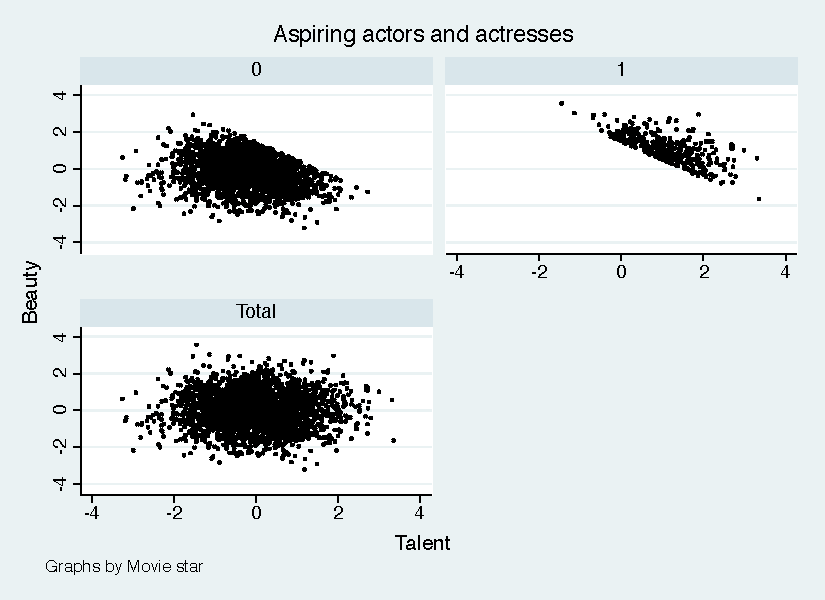
\includegraphics[height=9cm]{./lecture_includes/beauty_collider.pdf}
    \caption{Top left figure: Non-star sample scatter plot of beauty (vertical axis) and talent (horizontal axis). Top right right figure: Star sample scatter plot of beauty and talent.  Bottom left figure: Entire (stars and non-stars combined) sample scatter plot of beauty and talent.}
  \end{figure}
\end{frame}

\begin{frame}{Sample selection?}

\begin{itemize}
\item Notice that this is clear when we are focused on sample selection
\item But even a regression that included ``star'' would create the issue:$$beauty_i = \alpha + \delta talent_i + \beta star_i + \varepsilon_i$$
\item It's not just sample selection 
\end{itemize}

\end{frame}


\begin{frame}{Example 2: Discrimination}

  \begin{itemize}
    \item Let's look at another example: very common for think tanks and journalists to say that the gender gap in earnings disappears once you control for occupation.
    \item But what if occupation is a collider, which it could be in a model with occupational sorting
    \item Then controlling for occupation in a wage regression searching for discrimination can lead to all kinds of crazy results \emph{even in a simulation where we explicitly design there to be discrimination}
  \end{itemize}

\end{frame}

\begin{frame}{DAG}

  \begin{center}
    \begin{tikzpicture}
      [node distance=1.5cm]
      % nodes %
      \node[text centered] (f) {$F$};
      \node[above right of = f, text centered] (d) {$d$};
      \node[right of = f] (y) {$y$};
      \node[below  of = f, text centered] (o) {$o$};
      \node[right of = o, text centered] (a) {$A$};

      % edges %
      \draw[->, line width= 1] (f) -- (d);
      \draw[->, line width= 1] (d) -- (o);
      \draw[->, line width= 1, dashed] (a) -- (o);

      \draw[->, line width= 1] (d) -- (y);
      \draw[->, line width= 1] (o) -- (y);
      \draw[->, line width= 1, dashed] (a) -- (y);

    \end{tikzpicture}
  \end{center}

  $F$ is female, $d$ is discrimination, $o$ is occupation, $y$ is earnings and $A$ is ability. Dashed lines mean the variable cannot be observed. Note, by design, being a female has no effect on earnings or occupation, and has no relationship with ability. So earnings is coming through discrimination, occupation, and ability.

\end{frame}


\begin{frame}[plain]

  \begin{center}
    \begin{tikzpicture}
      [node distance=1.5cm]
      % nodes %
      \node[text centered] (f) {$F$};
      \node[above right of = f, text centered] (d) {$d$};
      \node[right of = f] (y) {$y$};
      \node[below  of = f, text centered] (o) {$o$};
      \node[right of = o, text centered] (a) {$A$};

      % edges %
      \draw[->, line width= 1] (f) -- (d);
      \draw[->, line width= 1] (d) -- (o);
      \draw[->, line width= 1, dashed] (a) -- (o);

      \draw[->, line width= 1] (d) -- (y);
      \draw[->, line width= 1] (o) -- (y);
      \draw[->, line width= 1, dashed] (a) -- (y);

    \end{tikzpicture}
  \end{center}


  Mediation and Backdoor paths

  \begin{enumerate}

    \item $d$ $\rightarrow o \rightarrow y$
    \item $d$ $\rightarrow o \leftarrow A \rightarrow y$
  \end{enumerate}

\end{frame}


\begin{frame}[plain, shrink=20]

  \begin{table}[htbp]\centering
    \scriptsize
    \caption{Regressions illustrating collider bias with simulated gender disparity}
    \begin{center}
      \begin{tabular}{l*{3}{c}}
        \toprule
        \multicolumn{1}{l}{Covariates: }&
        \multicolumn{1}{c}{\textbf{Unbiased combined effect}}&
        \multicolumn{1}{c}{\textbf{Biased }}&
        \multicolumn{1}{c}{\textbf{Unbiased wage effect only}}\\
        \midrule
        Female                     & -3.074*** & 0.601*** & -0.994*** \\
                                   & (0.000)   & (0.000)  & (0.000)   \\
        Occupation                 &           & 1.793*** & 0.991***  \\
                                   &           & (0.000)  & (0.000)   \\
        Ability                    &           &          & 2.017***  \\
                                   &           &          & (0.000)   \\
        \\
        \midrule
        N                          & 10,000    & 10,000   & 10,000    \\
        Mean of dependent variable & 0.45      & 0.45     & 0.45      \\
        \bottomrule
      \end{tabular}
    \end{center}
  \end{table}

  \begin{itemize}
    \item Recall we designed there to be a discrimination coefficient of -1
    \item If we do not control for occupation, then we get the combined effect of $d \rightarrow o \rightarrow y$ and $d  \rightarrow y$
    \item Because it seems intuitive to control for occupation, notice column 2 - the sign flips!
    \item We are only able to isolate the direct causal effect by conditioning on ability and occupation, but ability is unobserved
  \end{itemize}

\end{frame}

\begin{frame}[allowframebreaks,plain]

  \begin{itemize}
    \item \textbf{Colliders can be outcomes (and often those are the ones)}
          \begin{itemize}
            \item There is only one backdoor path from $D$ to $Y$

                  \begin{center}
                    \begin{tikzpicture}
                      [node distance=1.5cm]
                      % nodes %
                      \node[text centered,draw,rectangle,thin] (x1) {$X_1$};
                      \node[right of = x1, text centered] (d) {$D$};
                      \node[below right of = d, text centered] (x2) {$X_2$};
                      \node[above right of = x2, text centered] (y) {$Y$};

                      % edges %
                      \draw[->, line width= .5] (x1) -- (d);
                      \draw[->, line width= .5] (d) -- (y);
                      \draw[->, line width= .5] (d) -- (x2);
                      \draw[->, line width= .5] (y) -- (x2);
                      \draw[->, line width= .5] (x1) to [out=45,in=135, looseness=0.5] (y);
                    \end{tikzpicture}
                  \end{center}
                  

            \item Conditioning on $X_1$ blocks the backdoor path


            \item But what if we also condition on $X_2$?

                  \begin{center}
                    \begin{tikzpicture}
                      [node distance=1.5cm]
                      % nodes %
                      \node[text centered,draw,rectangle,thin] (x1) {$X_1$};
                      \node[right of = x1, text centered] (d) {$D$};
                      \node[below right of = d, draw, rectangle, text centered] (x2) {$X_2$};
                      \node[above right of = x2, text centered] (y) {$Y$};

                      % edges %
                      \draw[->, line width= .5] (x1) -- (d);
                      \draw[->, line width= .5] (d) -- (y);
                      \draw[->, line width= .5] (d) -- (x2);
                      \draw[->, line width= .5] (y) -- (x2);
                      \draw[->, line width= .5] (x1) to [out=45,in=135, looseness=0.5] (y);
                    \end{tikzpicture}
                  \end{center}

            \item Conditioning on $X_2$ opens up a new path, creating new spurious correlations between $D$ and $Y$ 
          \end{itemize}

          \framebreak


    \item \textbf{Colliders could be pre-treatment covariates (called M-bias because it looks like an M)}
          \begin{itemize}
            \item Name the backdoor paths.  Is it open or closed?

                  \begin{center}
                    \begin{tikzpicture}
                      [node distance=1.5cm, text centered]
                      % nodes %
                      \node[] (x) {$X$};
                      \node[above left of = x] (u1) {$U_1$};
                      \node[below left of = x] (u2) {$U_2$};
                      \node[right of = x] (d) {$D$};
                      \node[right of = d] (y) {$Y$};

                      % edges %
                      \draw[->, line width= .5, dashed] (u1) -- (x);
                      \draw[->, line width= .5, dashed] (u2) -- (x);
                      \draw[->, line width= .5, dashed] (u1) to [out=0,in=135, looseness=0.5] (y);
                      \draw[->, line width= .5, dashed] (u2) to [out=0,in=-135, looseness=0.5] (d);
                      \draw[->, line width= .5] (d) -- (y);
                    \end{tikzpicture}
                  \end{center}

            \item But what if we condition on $X$?

                  \begin{center}
                    \begin{tikzpicture}
                      [node distance=1.5cm, text centered]
                      % nodes %
                      \node[text centered,draw,rectangle,thin] (x) {$X$};
                      \node[above left of = x] (u1) {$U_1$};
                      \node[below left of = x] (u2) {$U_2$};
                      \node[right of = x] (d) {$D$};
                      \node[right of = d] (y) {$Y$};

                      % edges %
                      \draw[->, line width= .5, dashed] (u1) -- (x);
                      \draw[->, line width= .5, dashed] (u2) -- (x);
                      \draw[->, line width= .5, dashed] (u1) to [out=0,in=135, looseness=0.5] (y);
                      \draw[->, line width= .5, dashed] (u2) to [out=0,in=-135, looseness=0.5] (d);
                      \draw[->, line width= .5] (d) -- (y);
                    \end{tikzpicture}
                  \end{center}


          \end{itemize}
  \end{itemize}
  \framebreak


\end{frame}


\begin{frame}{Testing the Validity of the DAG}

  \begin{itemize}
    \item The DAG makes testable predictions
    \item Conditional on $D$ and $I$, parental education ($PE$) should no longer be correlated with $Y$
    \item Can be hard to figure this out by hand, but software can help (e.g., Daggity.net is browser based, Causal Fusion is more advanced)
    \item Causal algorithms tend to be DAG based and are becoming popular in industry 
  \end{itemize}

  \begin{center}
    \begin{tikzpicture}[node distance=1.5cm]
      % nodes %
      \node[text centered] (d) {$D$};
      \node[right of = d, text centered] (y) {$Y$};
      \node[above left of = d, text centered] (i) {$I$};
      \node[left of = i, text centered] (pe) {$PE$};
      \node[below of = pe, text centered] (b) {$B$};
      % edges %
      \draw[->, line width= 1] (d) -- (y);
      \draw[->, line width= 1,] (i) -- (d);
      \draw[->, line width= 1,] (pe) -- (i);
      \draw[->, line width= 1,] (pe) -- (d);
      \draw[->, line width= 1, dashed] (b) -- (pe);
      \draw[->, line width= 1, dashed] (b) -- (d);
      \draw[->, line width= .5] (i) to [out=45,in=135, looseness=0.5] (y);
    \end{tikzpicture}
  \end{center}

\end{frame}




\begin{frame}{Contrast this with ordinary practices}

\begin{itemize}
\item Person attempts to ``control for omitted variable bias'' by including as many ``controls'' as possible
\item Person does not even attempt to think about treatment assignment mechanism and therefore has no idea what variables are colliders, covariates or confounders
\item Machine learning can be ``naive'' too if the large dimension of features includes unknowingly colliders
\end{itemize}

\end{frame}

\begin{frame}{}

  \begin{figure}
    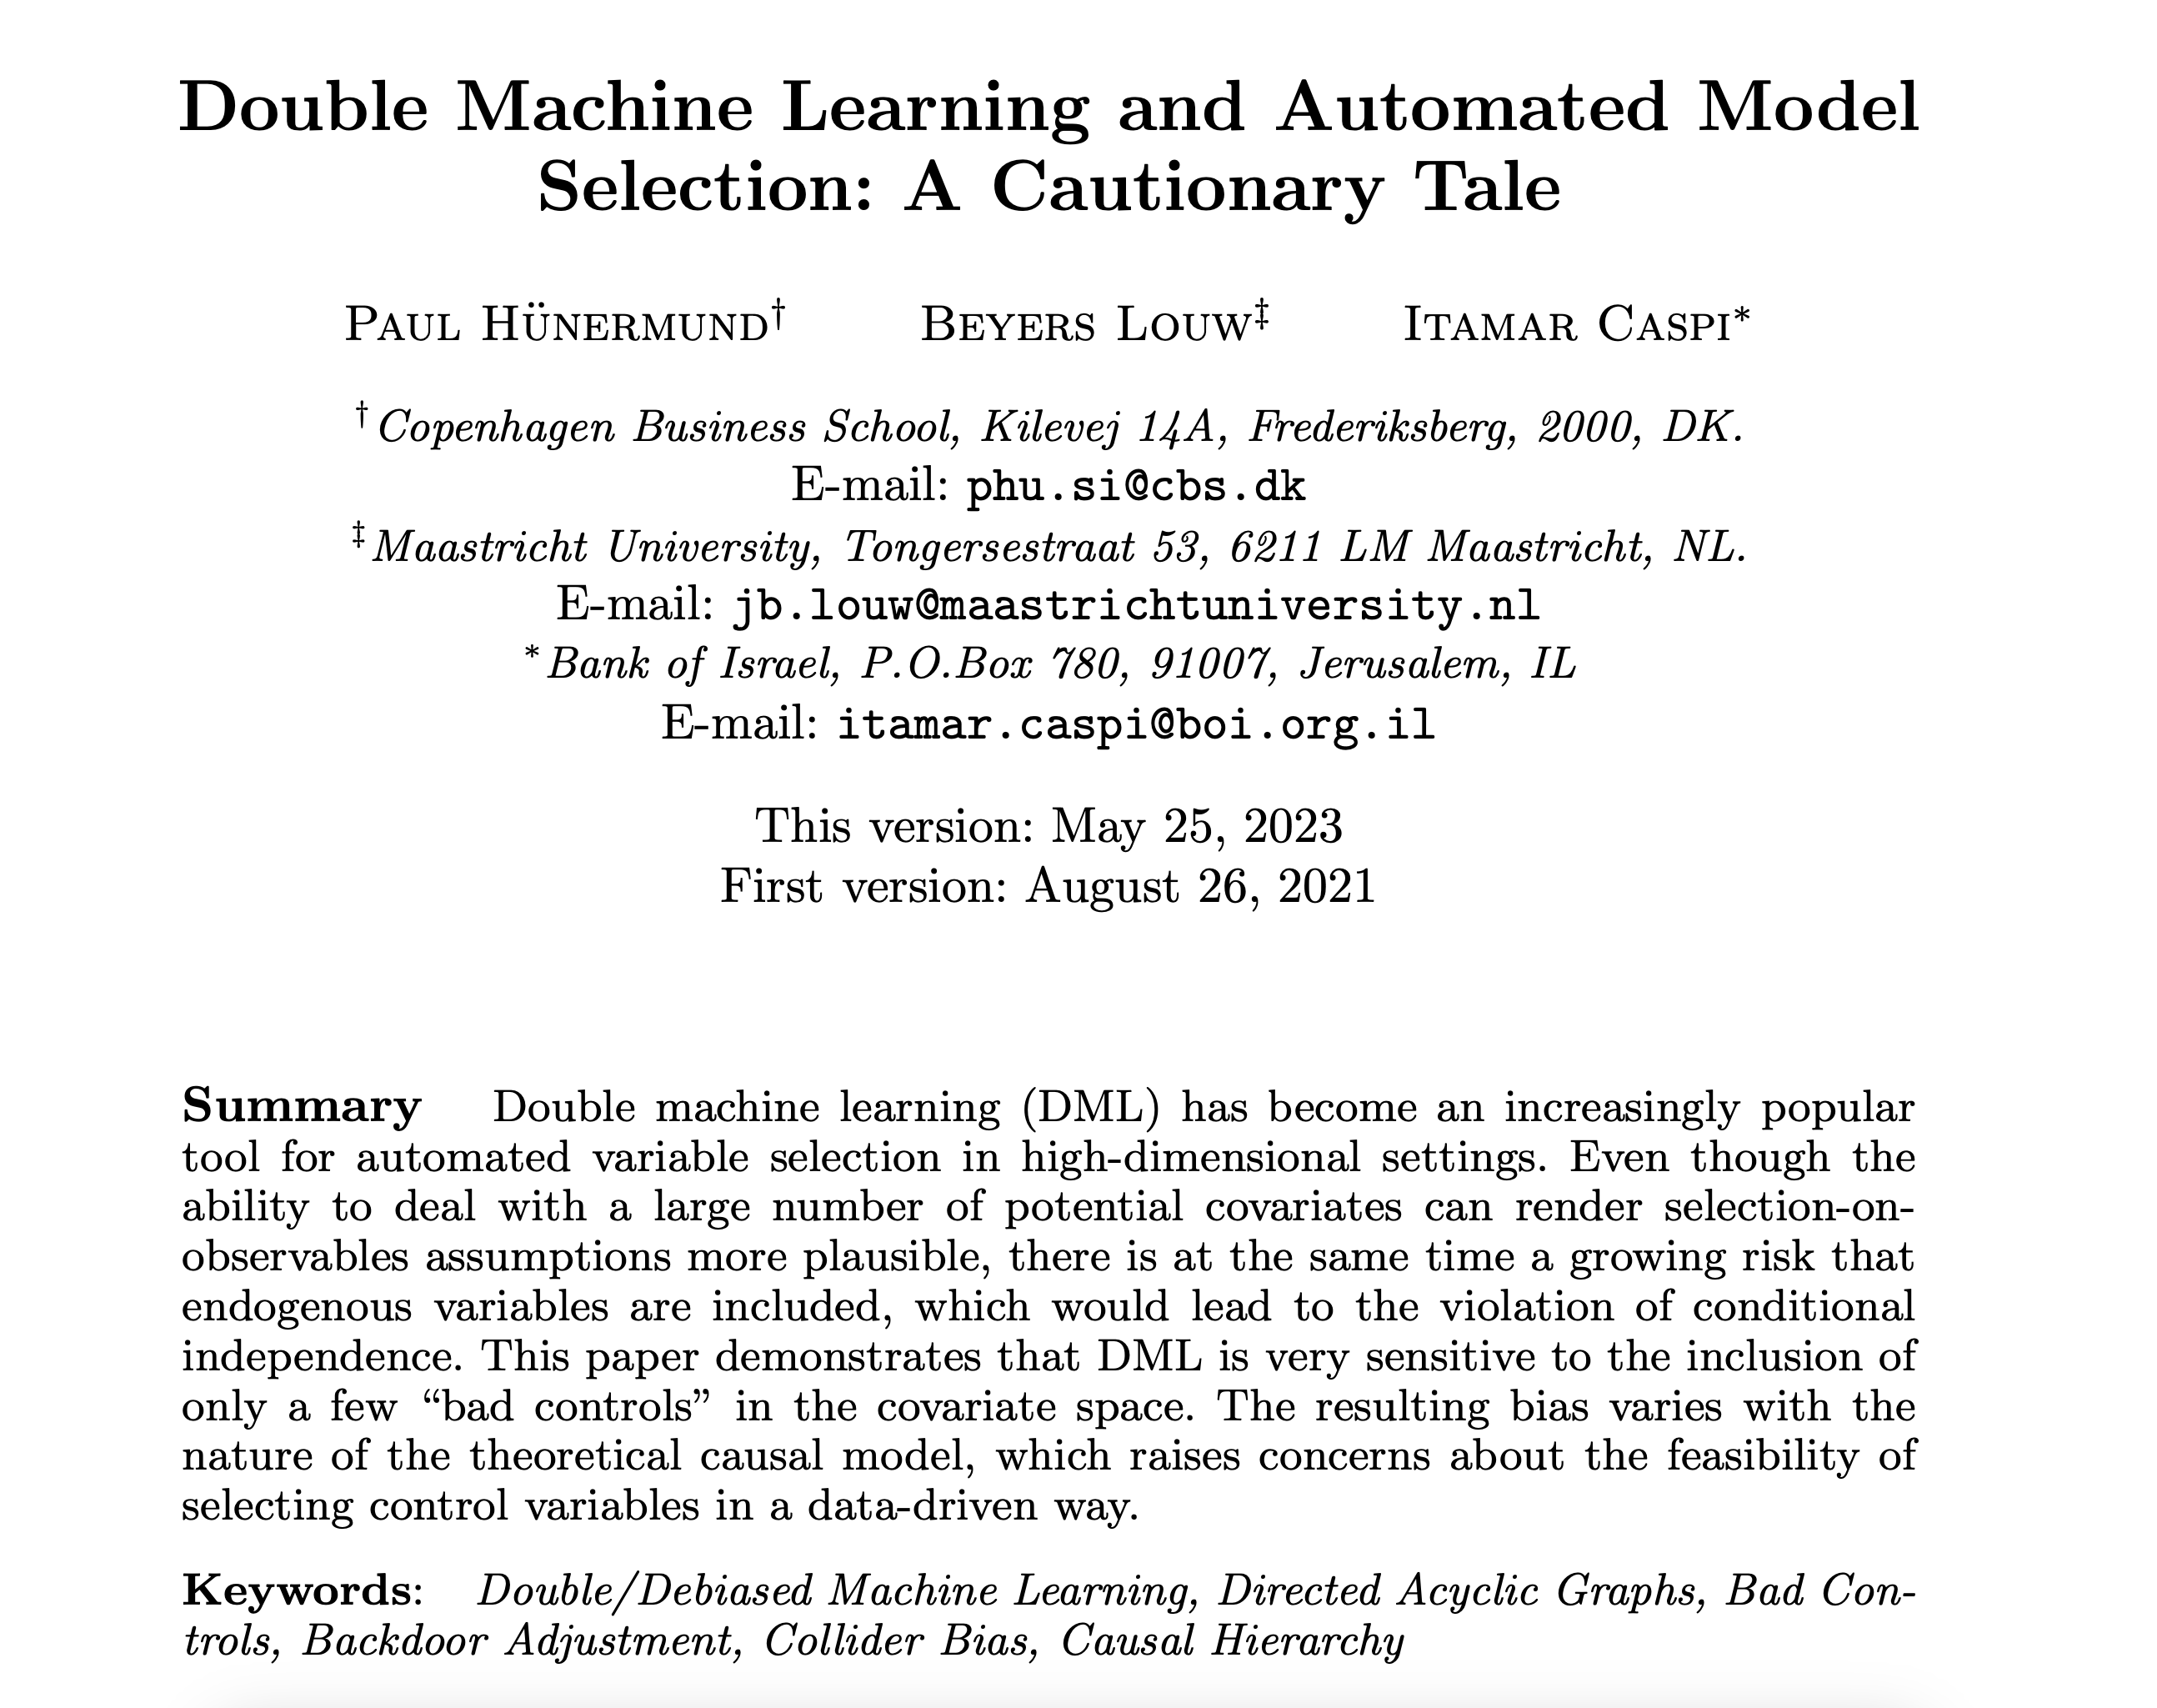
\includegraphics[scale=0.25]{./lecture_includes/paul_dml}
  \end{figure}

\end{frame}




\begin{frame}{Covariate selection without DAGs}

\begin{itemize}
\item What if you don't have a DAG you feel confident about?  
	\begin{enumerate}
	\item Include confounders that you feel pretty confident are there 
	\item Include covariates that are \emph{highly predictive} of the missing counterfactual (e.g., $Y^0$ for the ATT)
	\item Avoid outcomes (even though that still won't address M-bias colliders)
	\end{enumerate}
\item While this approach may be less formalized, you are at least reasoning about the treatment assignment mechanism as opposed to just including whatever variables you have laying around (avoid the ``kitchen sink regressions'')
\end{itemize}

\end{frame}

\begin{frame}{Falsifications as a test}

\begin{itemize}
\item Covariates should not be affected by the treatment, so examining them as falsifications can help establish the credibility of unconfoundedness
\item Imbens and Rubin (2015) suggested using the lagged outcome (pre-treatment) as a way of checking, as those have similar confounder structures
\item Falsifications too: One study questioned a finding that obesity was contagious in social networks by estimating the same model on things that cannot be contagious like acne, headaches and height and found the same things (likely confounding existed)
\end{itemize}

\end{frame}




\section{Unconfoundedness}

\subsection{Aggregate target parameters}

\begin{frame}{Shifting gears}

\begin{itemize}
\item Having reviewed the fundamentals of DAGs, we will now move into the practical realm
\item You have a non-experimental study.  
\item You have drawn your DAG or you have convinced yourself of your controls
\item We now discuss parameters, assumptions and estimation
\end{itemize}

\end{frame}



\begin{frame}{Known and Quantified Confounder}

	\begin{itemize}
	\item Confounders may or may not be observed,
	\item Confounders create backdoor paths between the treatment and the outcome
	\item Closing all backdoor paths to satisfy the backdoor criterion means that all remaining variation in the treatment is random
	\item One such set of design methods that utilize observed confounders to estimate causal effects are called ``unconfoundedness'' methods
	\end{itemize}

\end{frame}


\subsection{Aggregate treatment effect parameters}


\begin{frame}{Defining the target parameter comes first}

\begin{itemize}
\item Unconfoundedness methods include regression, weights or matching and they can be used to estimate average treatment effects like ATE, ATT, ATU
\item With constant treatment effects, they are the same ($ATE=ATT=ATU$) so methods that find one find all of them
\item Heterogenous treatment effects implies these will be different parameters, and thus different methods are needed
\item You must decide ahead of time which parameter you want to know in order to properly estimate it

\end{itemize}

\end{frame}



\subsection{Assumptions}


\begin{frame}{Aggregate causal parameters have missing potential outcomes}


\begin{itemize}
\item Every aggregate causal parameter is missing some potential outcome (e.g., ATT is missing $E[Y^0|D=1]$
\item If we are going to estimate the ATT, then it must be we are estimating $E[Y^0|D=1]$ somehow, but how?
\item If we are using observed confounders, then we are imputing the missing counterfactual using covariates in the comparison group
\item ``At some level, all methods for causal inference can be viewed as imputation methods, although some more explicitly than others.'' -- Imbens and Rubin (2015)

\end{itemize}


\end{frame}


\begin{frame}{Assumptions}

\begin{itemize}

\item When attempting to estimate aggregate causal parameters using covariate adjustment, we can do so with only two assumptions

	\begin{enumerate}
	\item \textbf{Unconfoundedness}:  fairly controversial to some because of what it implies about human behavior
	\item \textbf{Common support}: since most people stop at assumption 1, there's much less attention to common support
	\end{enumerate}
\item Today we will assume you satisfy unconfoundedness, and therefore our focus is on violations of assumption 2
\item Assuming constant treatment effects is unnecessary
\end{itemize}

\end{frame}


\begin{frame}[plain]

	\begin{block}{Identifying assumption I: Unconfoundedness}
	$(Y^0$, $Y^1)$ $\independent{D} | X$. There exists a set $X$ of known and quantified confounders such that after adjusting for them, treatment assignment is \emph{independent of potential outcomes}.
	\end{block}
	
	\begin{itemize}
	\item Conditional on $X$, treatment assignment is randomly distributed (i.e., independent of both potential outcomes) -- strong assumption
	\item For a large group of people within the same strata of $X$, this assumption states they choose treatments by flipping coins (not because they think the treatment helped them)
	\item Eliminating all backdoor paths on a DAG through blocking satisfies unconfoundedness; also called ignorability
	\end{itemize}
\end{frame}


\begin{frame}[plain]

	\begin{block}{Identifying assumption I: Unconfoundedness}
	$(Y^0$, $Y^1)$ $\independent{D} | X$. There exists a set $X$ of known and quantified confounders such that after adjusting for them, treatment assignment is \emph{independent of potential outcomes}.
	\end{block}
	
	\begin{eqnarray*}
	\alert{E[Y^0 | D=1, X=x]} &=& E[Y^0 | D=0, X=x] \\
	E[Y^1 | D=1, X=x] &=& \alert{E[Y^1 | D=0, X=x] }
	\end{eqnarray*}
	
Unconfoundedness justifies substituting units in treatment for control based on $X=x$ -- but only if there are exact matches
	
	
\end{frame}

\begin{frame}{Economic meaning of backdoor criterion}

\begin{itemize}
\item When people choose their own treatments, attempting to estimate aggregate causal parameters using covariates that conditional on those covariates, they are \emph{randomizing choices}
\item If people are optimizing, though, then it's a strong statement to claim that for groups of units with identical confounder values, they were choosing treatments based on coin flips
\end{itemize}

\end{frame}




\begin{frame}[plain]

	\begin{block}{Identifying assumption II: Common support}
	For ranges of $X$, there is a positive probability of being both treated and untreated
	\end{block}
	
	\begin{itemize}
	\item There exists units in treatment and control with same values of $X$ -- you can't make the substitutions otherwise
	\item Dimension $k$ means every specific combination of the conditioning set (e.g., not males and old, but adult males, adult females, youth male, youth female)
	\item Testable because common support is observable unlike unconfoundedness, but as you can imagine if the dimensions of $X$ gets large (and with a continuous covariate it's infinite!) then it won't hold in any finite sample!
	\end{itemize}
	
	
\end{frame}



\begin{frame}{Assumptions combined}
	
But if we have them both (represented below), we can even outside of an RCT estimate the ATE through nonparametric matching
  \begin{enumerate}
		\item $(Y^1,Y^0) \independent{D} | X$ (strong unconfoundedness)
		\item $0<Pr(D=1|X)<1$ with probability one (common support)
  \end{enumerate}

\bigskip
Comparing groups of individuals \emph{who have the same values of} $X$, treatment is no longer based gains, $\delta$. 

\bigskip

The second term implies we have people in treatment and control for every strata of $X$
\end{frame}


\begin{frame}{Estimating ATE with Assumptions}


	\begin{itemize}
	\item Unconfoundedness lets you use $Y^0_j$ from control group as $i$'s $\alert{Y^0_i}$ and $Y^1_i$ from treatment group as $j$'s $\alert{Y^1_j}$ using $X$ as the matching guide
		\begin{eqnarray*}
		E[Y^1-Y^0|X] &=& E[Y^1 - Y^0 | X,D=1] \\
		&=&E[Y|X,D=1] - E[Y|X,D=0]
		\end{eqnarray*}
	\item Common support (the bridge metaphor) allows the match to take place as well as weight over the covariate distribution 
		\begin{eqnarray*}
		\delta_{ATE} &=&E[Y^1-Y^0] = E\bigg[ E[Y^1 - Y^0 \ \vert \ X] \bigg] \\
		&=& \int E[Y^1 - Y^0 |X,D=1] dPr(X) \\
		&=& \int \left(E[Y|X,D=1] - E[Y|X,D=0]\right)dPr(X)
		\end{eqnarray*}
	\end{itemize}

\end{frame}



\begin{frame}{Maybe You Want the ATT}

ATE requires conditional independence with respect to both $Y^1$ and $Y^0$ which would mean complete irrationality 

\bigskip

If we want the ATT, we can go with strictly weaker assumptions -- weak unconfoundedness and weak overlap

\bigskip

One kind of selection: person  chooses the treatment based on what you gain, $Y^1$, but not what you lose, $Y^0$, and not net benefits, $\delta=Y^1-Y^0$

\end{frame}




\begin{frame}{ATT Identification}

We can modify those assumptions and weaken both which helps a lot

\begin{enumerate}
  \item $Y^0 \independent{D} | X$ (weak unconfoundedness)
  \item $Pr(D=1|X)<1$ (with $Pr(D=1)>0$) (weak support)
\end{enumerate}

\bigskip

We don't need full common support because we don't need to find counterfactuals for the control group -- we only need units in the control group that match with our treatment group

\bigskip

Selection is weaker too, like I said -- they are not entirely irrational, but who knows if it helps you

\end{frame}z



\begin{frame}{Estimating ATT}


Weighted averages under both assumptions:
		\begin{eqnarray*}
		\delta_{ATT} &=& \int \left(E[Y|X,D=1] - E[Y|X,D=0]\right)dPr(X|D=1)
		\end{eqnarray*}
We match units in treatment and control because under weak unconfoundedness they're substitutable, and we use weak common support so that we can actually do it, then we take weighted averages over the differences.  

\bigskip

What assumptions and method would you use to estimate the ATU?
		
\end{frame}



\begin{frame}{Estimators}

\begin{itemize}

\item Now we will explore estimators that for lack of a better word ``use covariates'' to estimate aggregate causal parameters
\item I will be bundling them around a few topics: exact matching, inexact matching, and regressions
\item Themes about heterogeneous treatment effects, common support and correct (and incorrect) regression specifications will be common

\end{itemize}

\end{frame}





\section{Estimators }


\subsection{Subclassification}

\begin{frame}{Causal inference using covariates}
\begin{itemize}

\item Multivariate regression goes back to Yule (19th century) and Fisher (20th century)
\item Subclassification was introduced by Cochran (late 60s)
\item Propensity score matching introduced early 80s (Rosenbaum and Rubin)
\item Regression based decomposition methods by Kitagawa (1950s), Oaxaca and Blinder (early 70s), and Kline, Wooldridge and others (in 00s)
\item Machine learning methods like double debiased ML by Chernozhukov, et al. (2018) and causal forests (Athey and Wager) 2018)
\end{itemize}

\end{frame}


\begin{frame}{Subclassification method}

\begin{itemize}

\item Wanting to show subclassification as an early effort to tackle covariates, but which ultimately cannot handle large features due to common support issues before moving into regression 
\item Titanic sank on maiden voyage April 15, 1912 after hitting an iceberg in North Atlantic
\item 2200 on board, but only 700 survived, despite 20 lifeboats with 60 capacity (1200 potential lives could've been saved)
\item Women and children first was a maritime rule to ration lifeboats, but there were different cabins (1st class, 2nd class, etc.) on different levels with different proximity to boats
\item What was the causal effect of 1st class on survival adjusting for $W$ and $C$?
\end{itemize}

\end{frame}


\begin{frame}{Titanic layout}
  \begin{figure}
    \begin{tikzpicture}
      \node[anchor=south west,inner sep=0] at (0,0) {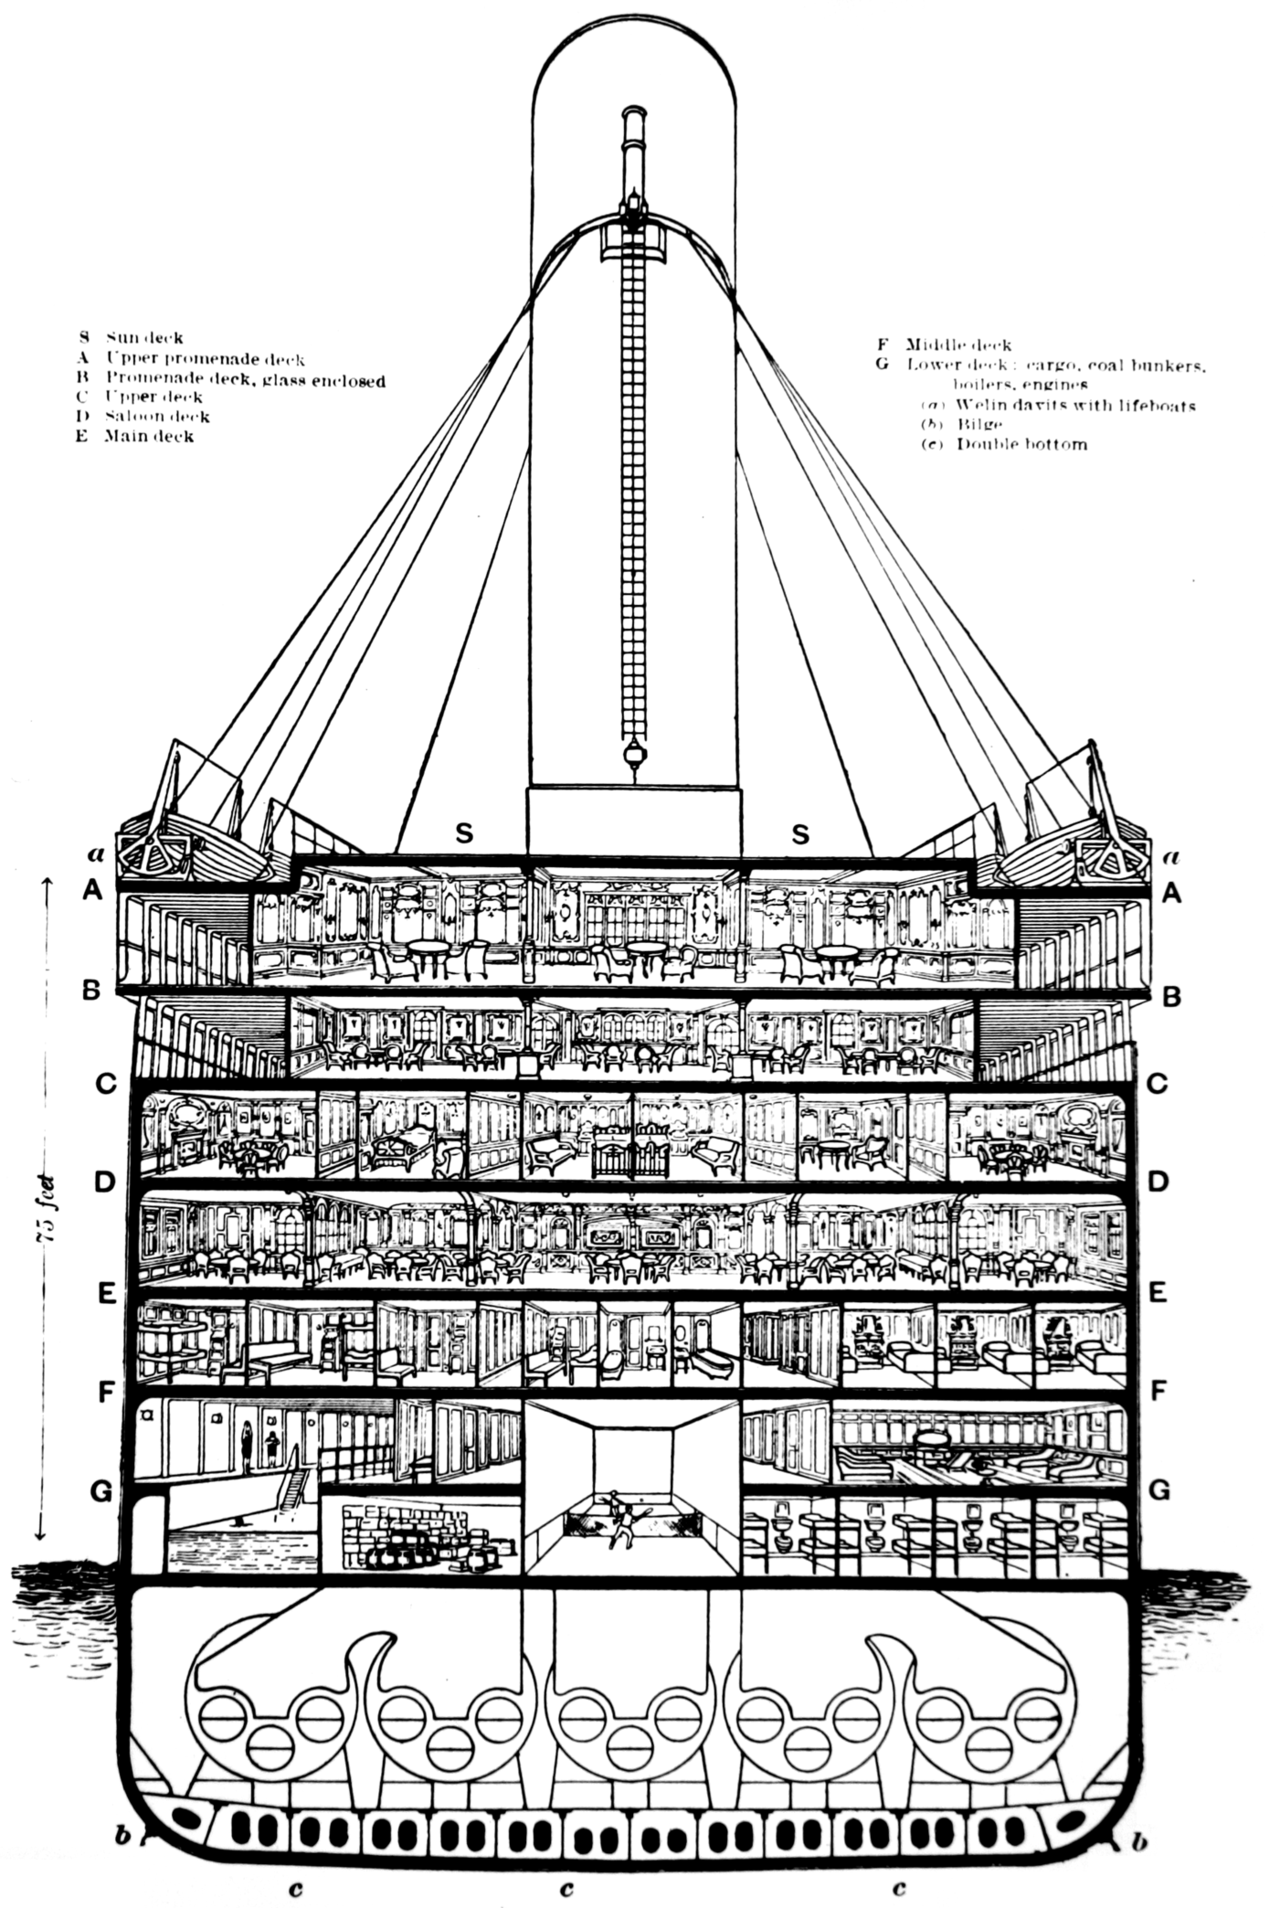
\includegraphics[scale=0.11]{./lecture_includes/titanic.png}};
      \draw[red,ultra thick,->] (6,4.25) -- (6,3.25); % Adjust the coordinates accordingly
      \node at (8,4.5) {First Class: Decks B-C}; % Adjust the position accordingly
    \end{tikzpicture}
  \end{figure}
\end{frame}

\begin{frame}{Titanic layout}
  \begin{figure}
    \begin{tikzpicture}
      \node[anchor=south west,inner sep=0] at (0,0) {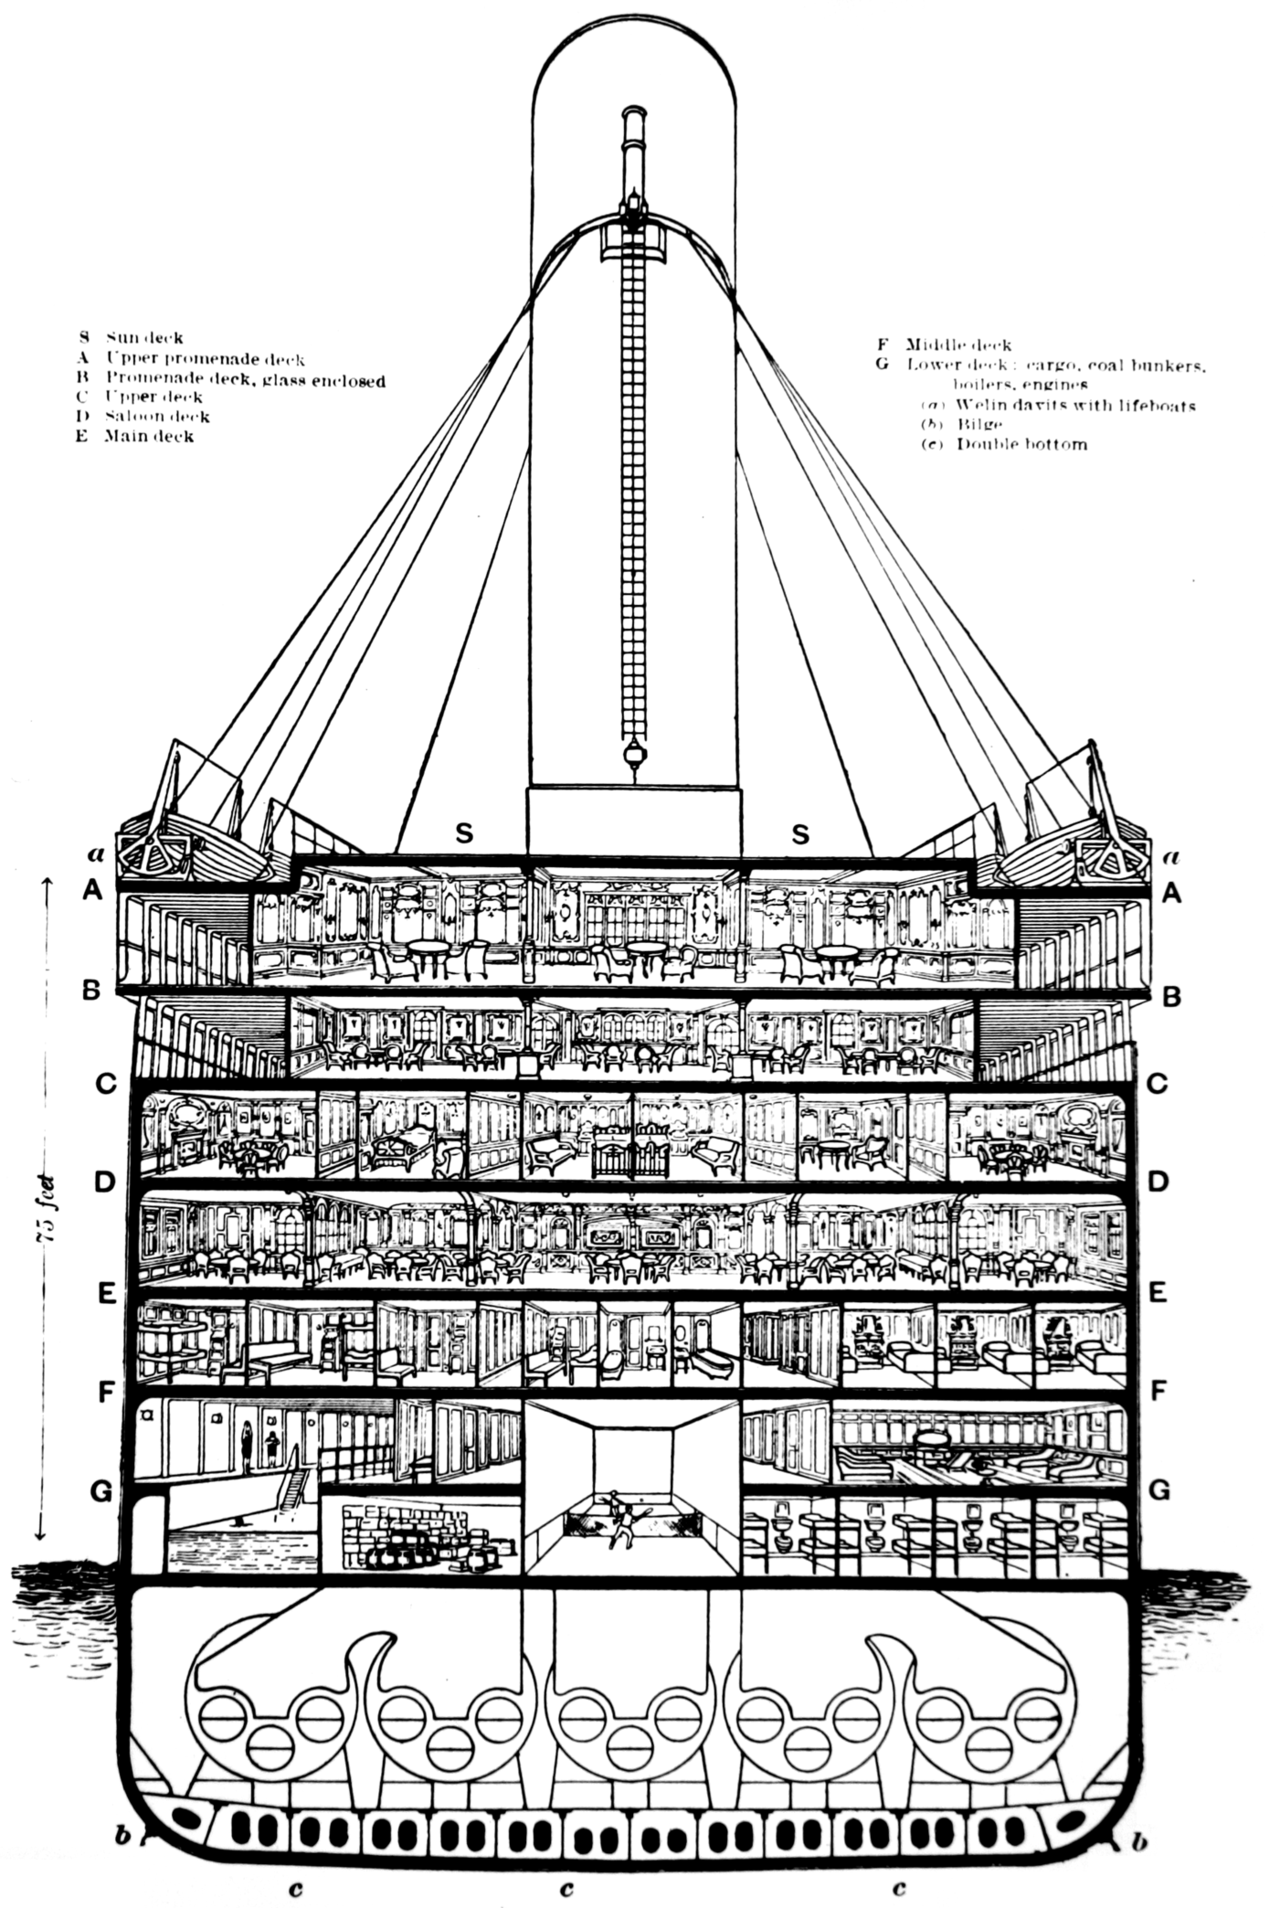
\includegraphics[scale=0.11]{./lecture_includes/titanic.png}};
      \draw[blue,ultra thick,->] (6,3.5) -- (6,2.5); % Adjust the coordinates accordingly
      \node at (8,4) {Second Class: Decks D-E}; % Adjust the position accordingly
    \end{tikzpicture}
  \end{figure}
\end{frame}

\begin{frame}{Titanic layout}
  \begin{figure}
    \begin{tikzpicture}
      \node[anchor=south west,inner sep=0] at (0,0) {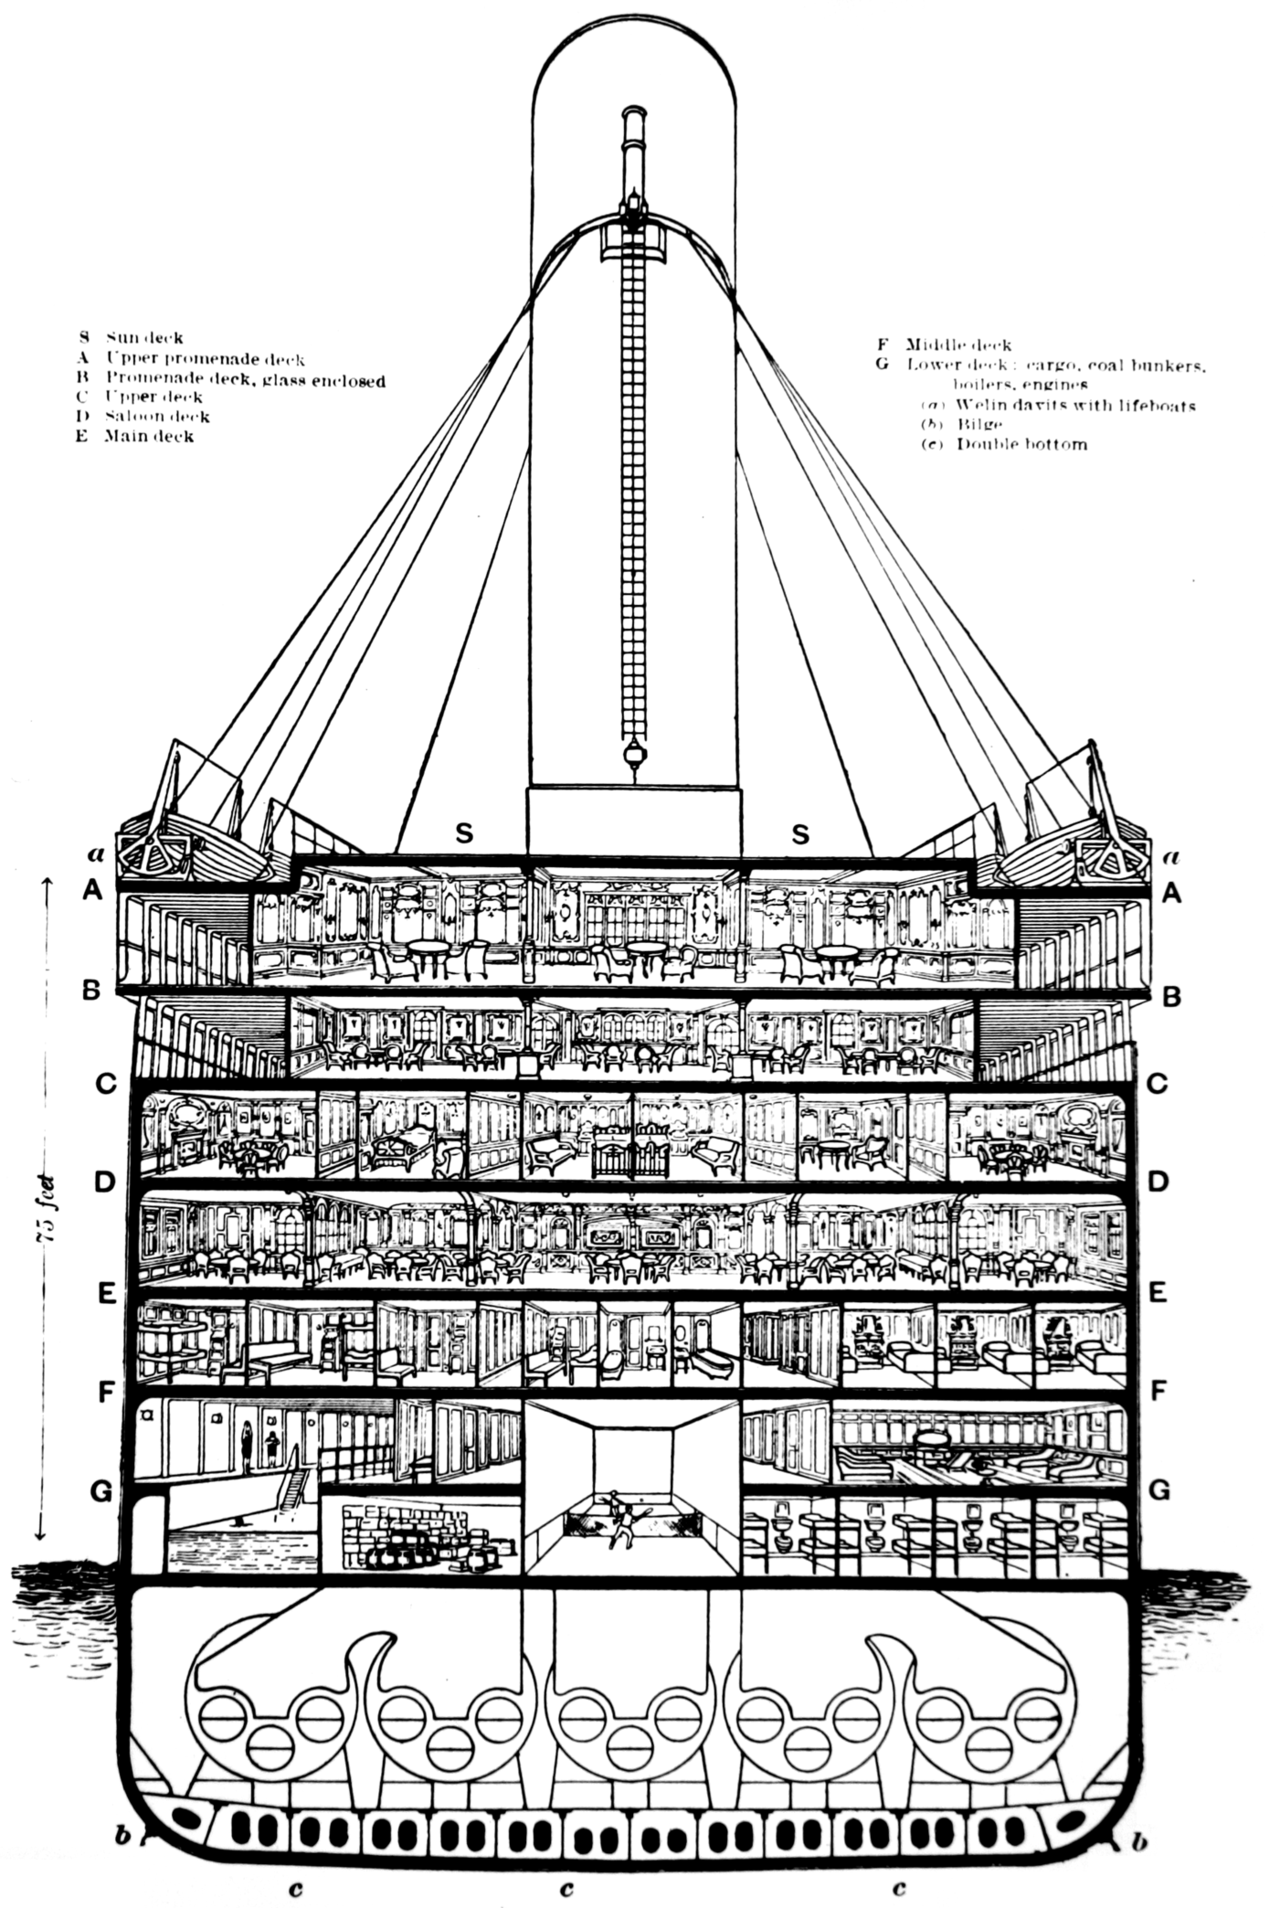
\includegraphics[scale=0.11]{./lecture_includes/titanic.png}};
      \draw[green,ultra thick,->] (6,2.25) -- (6,1.5); % Adjust the coordinates accordingly
      \node at (8,2.5) {Third Class: Decks F and G}; % Adjust the position accordingly
    \end{tikzpicture}
  \end{figure}
\end{frame}



\begin{frame}{Exercise: Titanic DAG}

\begin{figure}
\begin{center}
\caption{Women $W$ and children $C$ first maritime rule is a confounder for estimating first class $D$ effect on surviving $Y$}
\begin{tikzpicture}[node distance=2cm]
% nodes %
\node[text centered] (d) {$D$};
\node[below left of = d, text centered] (c) {$\mybox{C}$};
\node[above left of = d, text centered] (w) {$\mybox{W}$};
\node[right of = d, text centered] (y) {$Y$};
% edges %
\draw[->, line width= 1] (d) -- (y);
\draw[->, line width= 1] (c) -- (d);
\draw[->, line width= 1] (w) -- (d);
\draw[->, line width= 1] (c) -- (y);
\draw[->, line width= 1] (w) -- (y);
\end{tikzpicture}
\label{fig:titanic}
\end{center}
\end{figure}

\bigskip

Backdoor criterion can be satisfied by blocking on $W$ and $C$.  These are our known confounders.  Now we just need data to see if it's quantified.

\end{frame}

\begin{frame}{Titanic exercise}

\begin{enumerate}
\item \textbf{Stratify the confounders}: Our age and sex variables are both binary, so we can only create four strata: male children, female children, male adults, female adults
\item \textbf{Calculate differences within strata}: Calculate average survival rates for each group within each of the four strata and difference within strata
\item \textbf{Calculate probability weights}: Count the number of people in each strata and divide by the total number of souls aboard (crew and passengers)
\item \textbf{Aggregate differences across strata using weights}: Estimate the ATE by aggregating the difference in survival rates over the four strata with each strata-specific difference weighted by that strata's weight
\end{enumerate}


\end{frame}

\begin{frame}{Table 1: Typical balance table}

{\renewcommand{\arraystretch}{1.1}
\tabcolsep=1.3\tabcolsep 		
\begin{table}\small\index{rolling!3}
\caption{Differences in female and adult passengers by first class status on the Titanic. }
\centering
\begin{tabular}{lcc|cc}
\toprule
\multicolumn{1}{c}{\textbf{Variable name}}&
\multicolumn{2}{c}{\textbf{First class}}&
\multicolumn{2}{c}{\textbf{All other classes}}\\
\multicolumn{1}{c}{}&
\multicolumn{1}{c}{Obs}&
\multicolumn{1}{c}{Mean}&
\multicolumn{1}{c}{Obs}&
\multicolumn{1}{c}{Mean}\\
\midrule
Percent adult		&	325 	& 98.2\% & 1,876 & 94.5\% \\
Percent female		& 	325	& 44.6\% & 1,876 & 17.3\% \\
\bottomrule
\end{tabular}
\label{tab:titanic-age}
\end{table}}
\end{frame}


\begin{frame}{Table 2: Stratified sample}

{\renewcommand{\arraystretch}{1.1}
\tabcolsep=1.3\tabcolsep 		
\begin{table}\small\index{rolling!3}
\caption{Counts and Titanic survival rates by strata and first class status.}
\centering
\begin{tabular}{lcc|cc|c}
\toprule
\multicolumn{1}{c}{\textbf{}}&
\multicolumn{2}{c}{\textbf{First class}}&
\multicolumn{2}{c}{\textbf{All other classes}}&
\multicolumn{1}{c}{\textbf{}}\\
\multicolumn{1}{l}{Strata}&
\multicolumn{1}{c}{Obs}&
\multicolumn{1}{c}{Mean}&
\multicolumn{1}{c}{Obs}&
\multicolumn{1}{c}{Mean}&
\multicolumn{1}{c}{Total}\\
\midrule
Male adult		& 175	& 0.326	& 1,492	& 0.188	& 1,667 \\
Female adult	& 144	& 0.972	& 281	& 0.626	& 425 \\
Male child		& 5		& 1		& 59		& 0.407 	& 64\\
Female child	& 1		& 1		& 44		& 0.613 	& 45\\
\midrule
Total	observations	& 325	&&	1,876	 && 2,201\\
\bottomrule
\end{tabular}
\label{tab:titanic-counts}
\end{table}}


\end{frame}

\begin{frame}{Table 3: Estimates of aggregate parameters}

{\renewcommand{\arraystretch}{1.1}
\tabcolsep=1.3\tabcolsep 		
\begin{table}\tiny\index{rolling!3}
\caption{Differences in survival rates, stratification weights, and estimates of parameters}
\centering
\begin{tabular}{lc|ccc}
\toprule
\multicolumn{1}{l}{\textbf{Strata}}&
\multicolumn{1}{c}{\textbf{Differences in Survival Rates}}&
\multicolumn{1}{c}{\textbf{Weight$_{k,ATE}$}}&
\multicolumn{1}{c}{\textbf{Weight$_{k,ATT}$}}&
\multicolumn{1}{c}{\textbf{Weight$_{k,ATU}$}}\\
\midrule
Male adult		& 0.138 &	0.76 &	0.54	&0.80	\\
Female adult	& 0.346 &	0.19 &	0.44	&0.15	\\
Male child		& 0.593 &	0.03 &	0.02	&0.03	\\
Female child	& 0.387 &	0.02 &	0.00	&0.02	\\
\midrule
\multicolumn{1}{l}{\textbf{}}&
\multicolumn{1}{c}{\textbf{No stratification}}&
\multicolumn{3}{c}{\textbf{Stratification weighted estimates}}\\

 & $\widehat{\textbf{SDO}}$& $\widehat{\textbf{ATE}}$ & $\widehat{\textbf{ATT}}$ & $\widehat{\textbf{ATU}}$ \\
\midrule
\textbf{Estimated coefficient}& 0.35 & 0.20 & 	0.24	 & 0.19   \\
\bottomrule
\end{tabular}
\label{tab:titanic-weights}
\end{table}}



\end{frame}



\begin{frame}{Drop the one female child}

\begin{itemize}
\item We were able to estimate all three causal effect parameters because for all four strata there were units in both treatment and control
\item But if we dropped the only female child in first class from the data, we'd be in trouble bc there wouldn't be any way to calculate a difference for that group
\item But what could we identify?

\end{itemize}

\end{frame}

\begin{frame}

\begin{table}\small\index{rolling!3}
\caption{Counts and Titanic survival rates by strata and first class status.}
\centering
\begin{tabular}{lcc|cc|c}
\toprule
\multicolumn{1}{c}{\textbf{}}&
\multicolumn{2}{c}{\textbf{First class}}&
\multicolumn{2}{c}{\textbf{All other classes}}&
\multicolumn{1}{c}{\textbf{}}\\
\multicolumn{1}{l}{Strata}&
\multicolumn{1}{c}{Obs}&
\multicolumn{1}{c}{Mean}&
\multicolumn{1}{c}{Obs}&
\multicolumn{1}{c}{Mean}&
\multicolumn{1}{c}{Total}\\
\midrule
Male adult		& 175	& 0.326	& 1,492	& 0.188	& 1,667 \\
Female adult	& 144	& 0.972	& 281	& 0.626	& 425 \\
Male child		& 5		& 1		& 59		& 0.407 	& 64\\
Female child	& 0		& n/a		& 44		& 0.613 	& 44\\
\midrule
Total	observations	& 324	&&	1,876	 && 2,200\\
\bottomrule
\end{tabular}
\label{tab:titanic-counts2}
\end{table}

\end{frame}

\begin{frame}{ATT is the only one we can get}

\begin{eqnarray}
\widehat{\delta}_{ATT} &=& (0.137 \times 0.54) + (0.346 \times 0.44) + (0.593 \times 0.02)  \nonumber \\
&=& 0.24\text{ or 24 percentage points}
\end{eqnarray}

\end{frame}

\begin{frame}

\begin{table}\tiny\index{rolling!3}
\caption{Differences in survival rates, stratification weights, and estimates of parameters without perfect stratification}
\centering
\begin{threeparttable}
\begin{tabular}{lc|ccc}
\toprule
\multicolumn{1}{l}{\textbf{Strata}}&
\multicolumn{1}{c}{\textbf{Differences in Survival Rates}}&
\multicolumn{1}{c}{\textbf{Weight$_{k,ATE}$}}&
\multicolumn{1}{c}{\textbf{Weight$_{k,ATT}$}}&
\multicolumn{1}{c}{\textbf{Weight$_{k,ATU}$}}\\
\midrule
Male adult		& 0.137 	&	0.76 &	0.54	&0.80	\\
Female adult	& 0.346 	&	0.19 &	0.44	&0.15	\\
Male child		& 0.593 	&	0.03 &	0.02	&0.03	\\
Female child	& n/a 	&	n/a 	&	n/a	&0.02	\\
\midrule
\multicolumn{1}{l}{\textbf{}}&
\multicolumn{1}{c}{\textbf{No stratification}}&
\multicolumn{3}{c}{\textbf{Stratification weighted estimates}}\\

 & $\widehat{\textbf{SDO}}$& $\widehat{\textbf{ATE}}$ & $\widehat{\textbf{ATT}}$ & $\widehat{\textbf{ATU}}$ \\
\midrule
\textbf{Estimated coefficient}& 0.35 & n/a & 	0.24	 & n/a  \\
\bottomrule
\end{tabular}
\begin{tablenotes}
\tiny
\item 
Differences in survival rates, stratification weights, and estimated parameters. All coefficients should be multiplied by 100 to get a percentage point change in survival rate as a result of having a first class cabin. Note that the SDO is a simple difference in mean outcomes and therefore \emph{not} a weighted average over the strata differences.  But the estimated ATE, ATT and ATU parameters are weighted averages in difference in means using corresponding stratification weights. 
\end{tablenotes}
\end{threeparttable}
\label{tab:titanic-weights2}
\end{table}


\end{frame}

\begin{frame}{Why did this happen?}

\begin{itemize}

\item Stratification requires having units in both groups for every value of $X$ to get ATE
\item If you want the ATT, you have to have units in the control group for every treated group based on its value of $X$ (female children weren't treated, so didn't matter)
\item If you want the ATU, you have to have units in the treatment group for every treated group based on its value of $X$ (female children weren't treated, so did matter)
\item This has a technical word we are going to learn more about called a ``lack of common support''
\end{itemize}

\end{frame}

\begin{frame}{Curse of Dimensionality}
	
	\begin{itemize}
	\item Stratification methods break down in finite samples because as increase the number of covariates, the "dimension" grows even faster -- dimensions and covariates aren't the same in other words
	\item Assume we have $k$ covariates and we divide each into 3 coarse categories (e.g., age: young, middle age, old; income: low, medium, high, etc.)
	\item The number of strata is $3^k$. For $k=10$, then it's $3^{10}=59,049$
	\item The curse of dimensionality is based on the slices of all interactions of the covariates, not just the covariates, and that explodes fast
	\end{itemize}
\end{frame}

\begin{frame}{Empty cells}
	
	\begin{itemize}
	\item When some slice is empty, it means there's no one in that cell -- so maybe you don't have any female children in first class, but you do have them in other cabins
	\item When you have empty cells, you can't match within that dimension of the data, and so the "curse of dimensionality" is one of the reasons why the kitchen sink approach breaks down so fast
	\item Matching methods really force us to see these curses; they're often hidden from OLS because OLS (as we'll see) overcomes the problem by just assuming a linearity (it doesn't match; it extrapolates)
	\end{itemize}
\end{frame}	





\subsection{Exact and Inexact Matching}

\begin{frame}{Common Support vs No Common Support}
    \begin{columns}
        \column{0.5\linewidth}
        \centering
        
\includegraphics[height=6.5cm, width=5.5cm]{./lecture_includes/romans_commonsupport.png}

        \column{0.5\linewidth}
        \centering
        
\includegraphics[height=6.5cm, width=5.5cm]{./lecture_includes/romans_nosupport.png}
    \end{columns} 
\end{frame}

\begin{frame}{Common support vs no common support}

\begin{itemize}
\item Common support is what will determine unbiasedness in nonparametric methods that satisfy unconfoundedness
\item Strictly speaking common support will mean that we have \emph{exact} matches
\item When we have inexact matches, then nonparametric matching methods may become biased
\item Some bias adjustment methods can improve estimation
\item We'll review these all now
\end{itemize}

\end{frame}



\begin{frame}{Exact matching}

\begin{figure}[!t]\centering
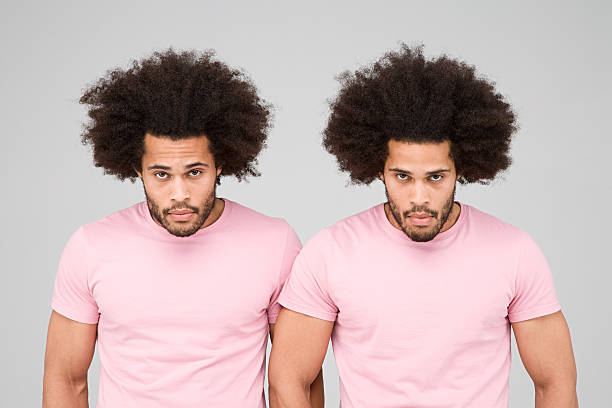
\includegraphics[scale=1.1]{./lecture_includes/identical_twins}
\end{figure}

\end{frame}

\begin{frame}{Exact Matching}


Matching goes back at least to Rubin's early work on the propensity score, but we will start with nearest neighbor matching as there's ideas there we draw upon later with synth I want to emphasize

\bigskip

Matching will match a treated unit to a comparison unit that is identical on the known and quantified confounders

\bigskip

If we can't find one, it means common support failed, the estimate would need to use nearest neighbors (with matching bias), which we will discuss



\end{frame}



\begin{frame}{Training example (unmatched)}

\begin{figure}[!t]\centering
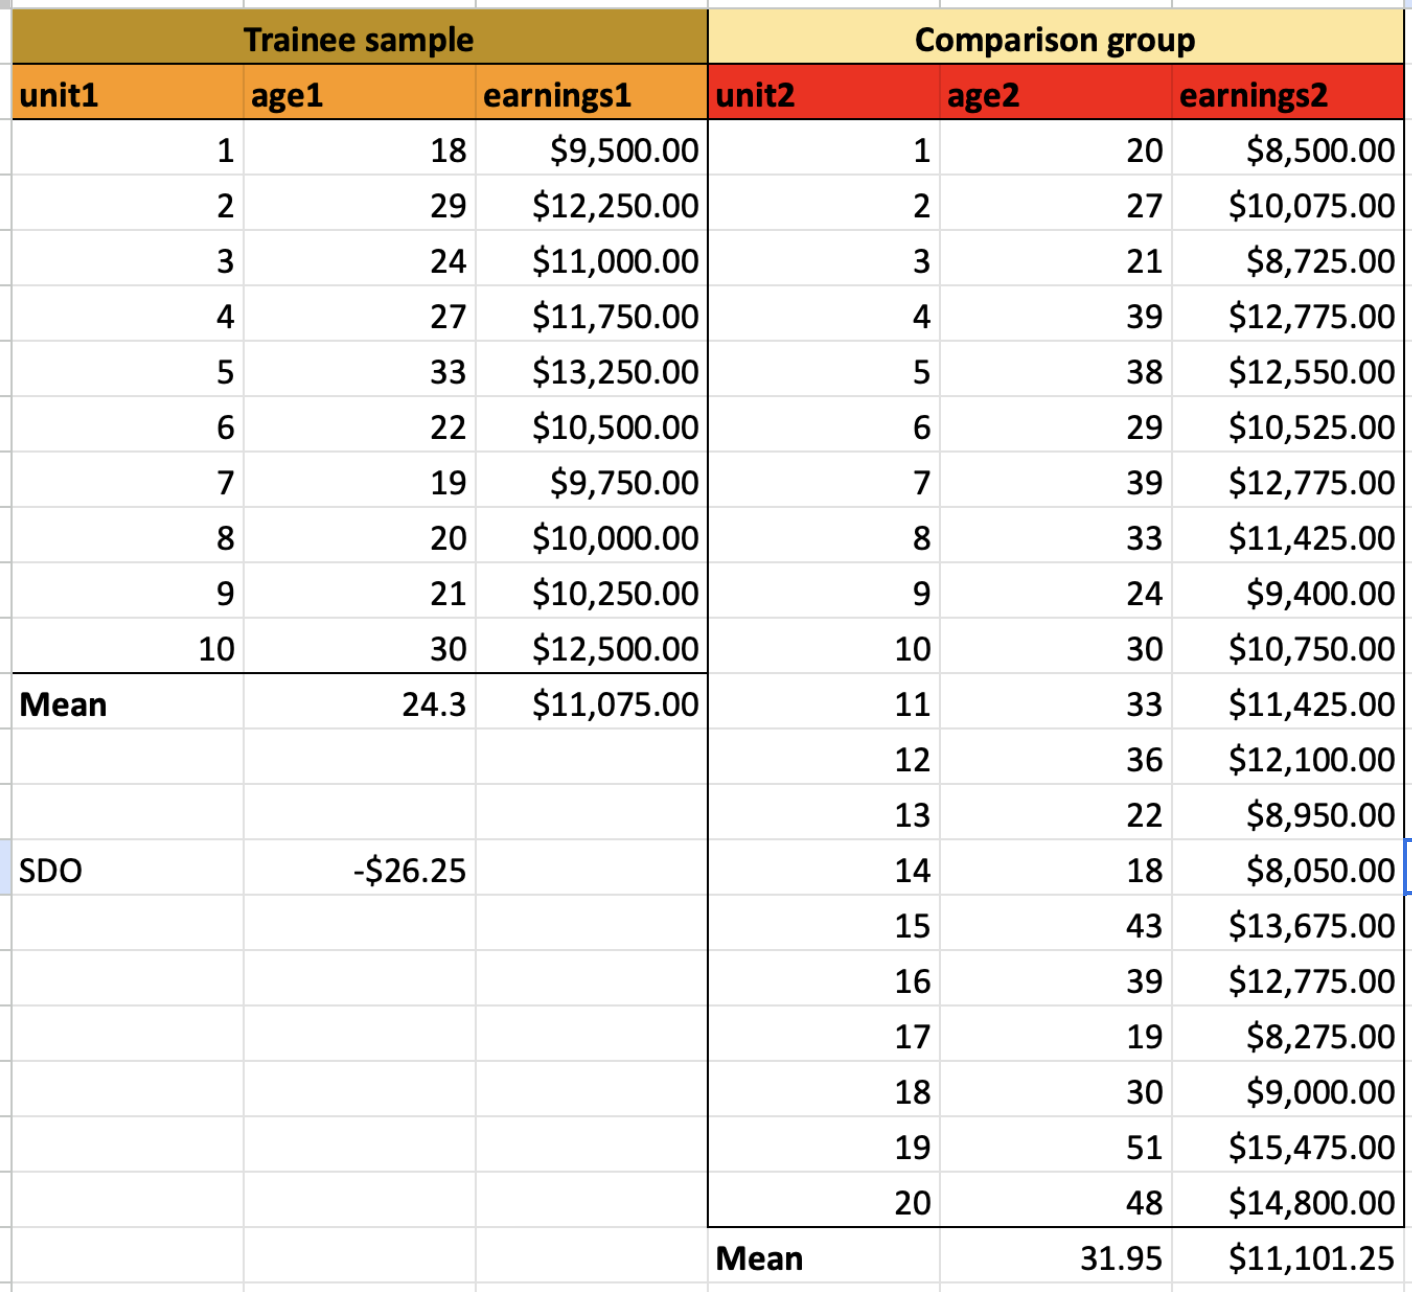
\includegraphics[scale=0.35]{./lecture_includes/raw_example}
\end{figure}


\end{frame}


\begin{frame}{Age Imbalance}

\begin{figure}[!t]\centering
\caption{Age distribution of a job training program's trainees (green) versus a sample of workers who were not enrolled in the trainee program (white).}
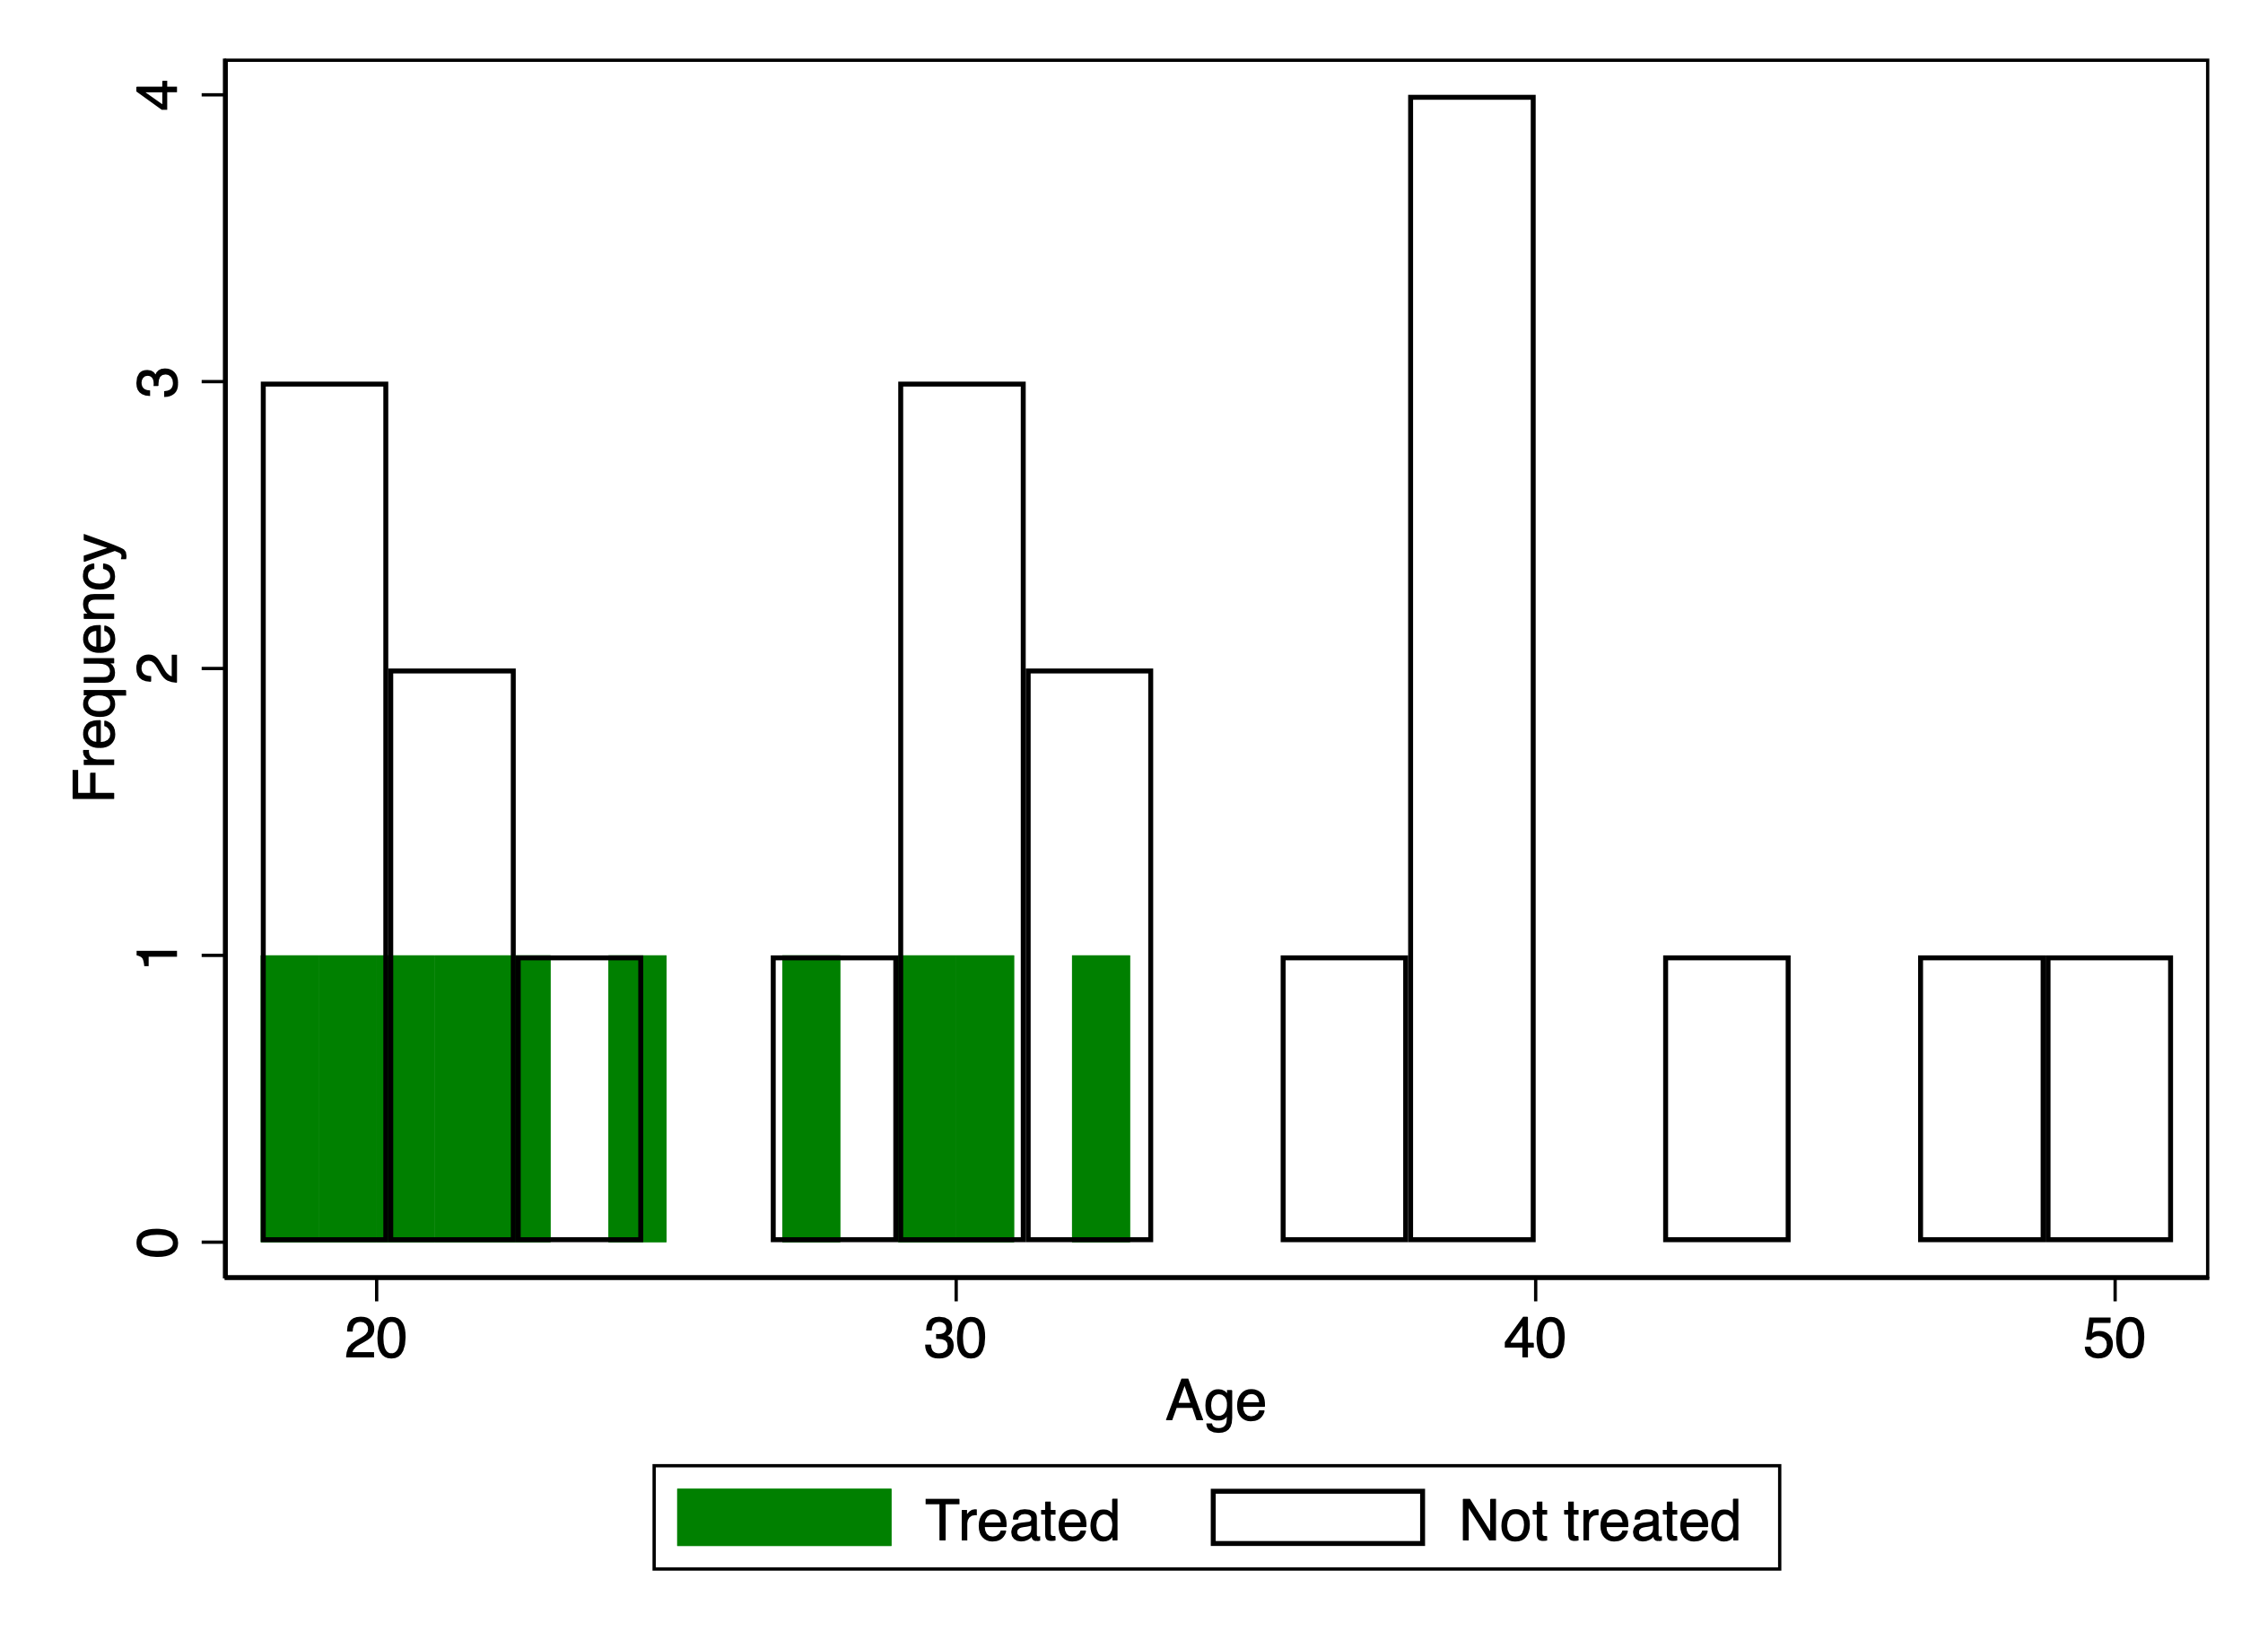
\includegraphics[scale=0.20]{./lecture_includes/age_match.png}
\end{figure}

\end{frame}


\begin{frame}{Exact matching}

\begin{itemize}
\item Exact matching finds a person in the control group whose value of $X_j$ is \emph{exactly} equal to each person in the treatment group $i$
\item Will not work if the conditioning set includes a continuous variable
\item Will also not work if $K$ gets large (curse of dimensionality we discuss later)
\end{itemize}

\end{frame}



\begin{frame}{ATT estimator}

We will focus on the ATT for the rest of today and the equation is:

\begin{equation}
\widehat{\delta}_{ATT} = \dfrac{1}{N_T} \sum_{D_i=1}(Y_i - Y_{j(i)})
\label{eq:att_simplematch}
\end{equation}

where $Y_{j(i)}$ is the $j$\textsuperscript{th} unit matched to the $i$\textsuperscript{th} unit based on the $j$\textsuperscript{th} being ``exactly equal to'' the $i$\textsuperscript{th} unit with respect to the $X$ conditioning set

\end{frame}

\begin{frame}{Number of matches}

What if I find two or more $M$ units with the identical $X$ value? Then what?

\begin{equation}
\widehat{\delta}_{ATT} = \dfrac{1}{N_T} \sum_{D_i=1} \bigg ( Y_i - \bigg [\dfrac{1}{M} \sum_{m=1}^M Y_{j_m(1)} \bigg ] \bigg )
\label{eq:att_match}
\end{equation}

\bigskip

Notice that we are only dealing with $Y^0_i$ by matching; The $Y^1_i$ is fine as is.

\end{frame}

\begin{frame}{Matching algorithm}

\begin{enumerate}
\item For each unit $i$ in the treatment group with known and quantified confounder $X=x_i$, find all units $j$ in the donor pool for whom $x_i=x_j$. These $j$ units are our $M$ matches and $M$ can be one or it can be greater than one if you want it to be.
\item For each unit $i$, replace its missing potential outcome, $Y^0_i$, with the matched $j$ units' realized outcomes, $\frac{1}{M} \sum {Y}_{j(i)}$, from Step 1. Do this for all $i$ units in the treatment group.
\item For each unit $i$, calculate the difference between realized earnings and matched earnings, $\widehat{\delta}_i=Y_i - \frac{1}{M} \sum {Y}_{j(i)}$.
\item Finally, estimate the sample ATT by averaging over all $i$ differences in earnings from Step 3 as $\frac{1}{N_T} \sum \widehat{\delta}_i$, where $N_T$ is the number of treatment units.
\end{enumerate}

\end{frame}



\begin{frame}{Matched sample}

\begin{figure}[!t]\centering
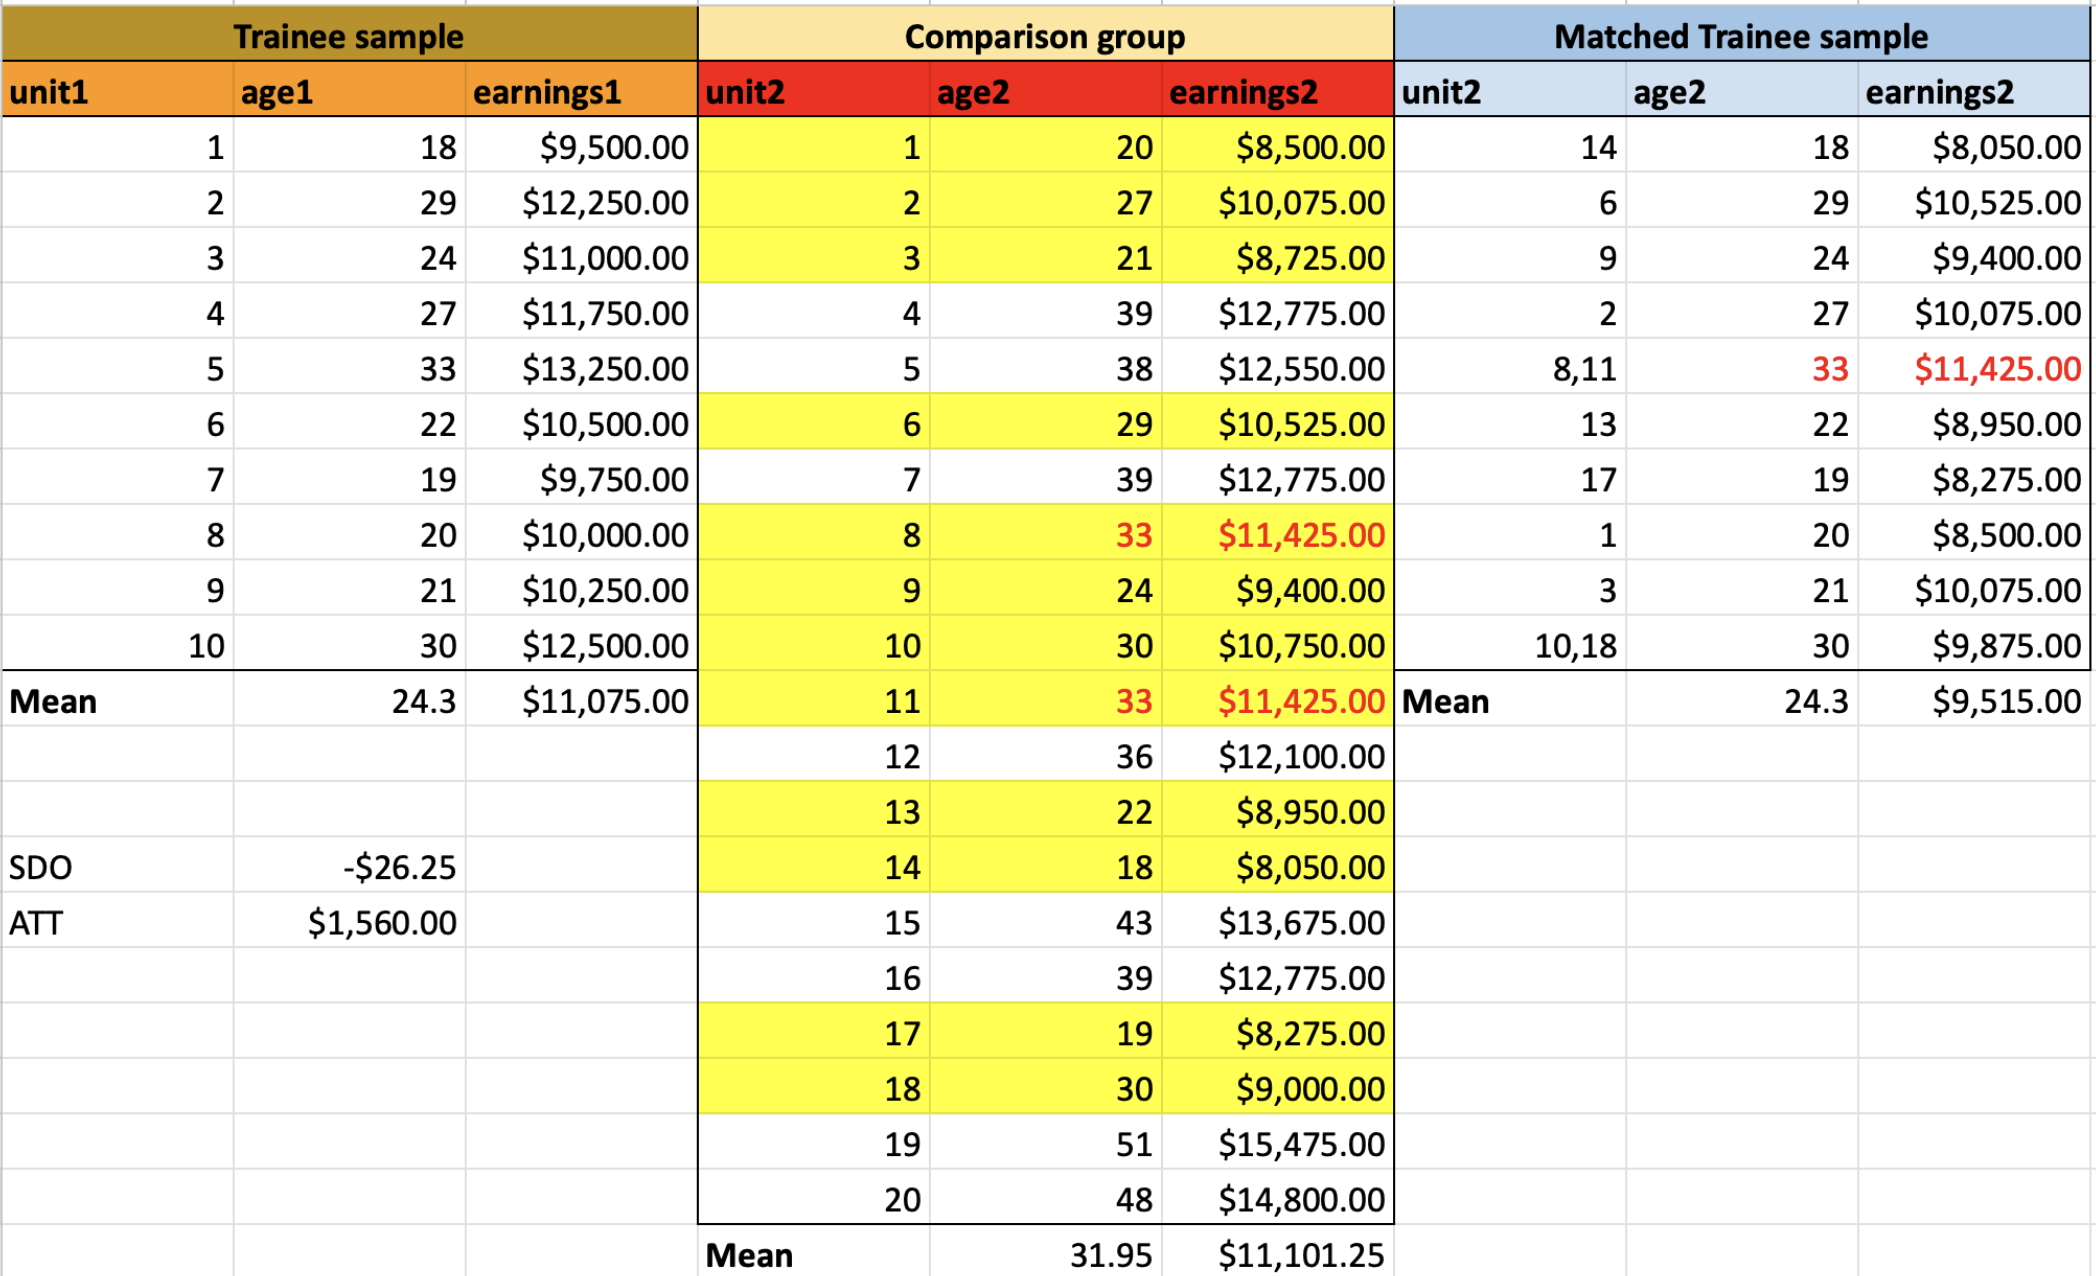
\includegraphics[scale=0.3]{./lecture_includes/matched_example}
\end{figure}



\end{frame}

\begin{frame}{Estimated ATT using Exact Matching}


\begin{itemize}
\item Weak unconfoundedness of $Y^0$ with respect to age justifies substituting the comparison group for the missing treatment group $$\textcolor{red}{E[Y^0|D=1, X=x]} = E[Y^0|D=0, X=x]$$
\item But unbiasedness requires exact matches -- unconfoundedness is necessary but not sufficient -- as we have to replace exactly on X
\item Even weak support is rare due to the curse of dimensionality
\end{itemize}

\end{frame}





\begin{frame}{Inexact matching}

\begin{figure}[!t]\centering

\includegraphics[scale=0.75]{./lecture_includes/fraternal_twins}
\end{figure}

\end{frame}


\begin{frame}{Curse of Dimensionality}
	
	\begin{itemize}
	\item If no matches can be found, it means many cells may contain either only treatment units or only control units but not both, and that violates our common support assumption
	\item We can always use ``finer'' classifications, but finer cells worsens the dimensional problem, so we don't gain  much from that.  ex: using $10$ variables and $5$ categories for each, we get $5^{10} = 9,765,625$.  
	\item Matching methods really force us to see these curses; they're hidden with regressions because OLS imputes missing counterfactuals based off the linear functional form
	\end{itemize}
\end{frame}	





\begin{frame}{To Look Like Someone Else}

\begin{itemize}
\item When we can make synthetic xerox copies of ourselves, that's exact matching
\item But what if we can only make similar copies of ourselves, like fraternal, but not identical, twins? That's nearest neighbor matching -- a form of ``inexact matching'', sort of like fraternal twins
\item Introduces possible bias depending on heterogenous treatment effects, but the magnitude of the bias depends on the severity of the matching discrepancy
\item We can improve on nearest neighbor matching using bias adjustment (Abadie and Imbens 2011) which uses an outcome regression to estimate the bias
\end{itemize}

\end{frame}

\begin{frame}{Nearest Neighbor Matching}
	
	\begin{itemize}
	\item Estimate $\widehat{\delta}_{ATT}$ by \emph{imputing} the missing potential outcome of each treatment unit $i$ using the observed outcome from that outcome's ``nearest'' neighbor $j$ in the control set using $X$ for the matching
		\begin{eqnarray*}
		\widehat{\delta}_{ATT} = \frac{1}{N_T}\sum_{D_i=1} (Y_i - Y_{j(i)})
		\end{eqnarray*}where $Y_{j(i)}$ is the observed outcome of a control unit such that $X_{j(i)}$ is the \textbf{closest} value to $X_i$ among all of the control observations (eg match on $X$)
	\end{itemize}
\end{frame}

\begin{frame}{Matching}
	
	\begin{itemize}
	\item We could also use the average observed outcome over $M$ closest matches:
		\begin{eqnarray*}
		\widehat{\delta}_{ATT} = \frac{1}{N_T}\sum_{D_i=1}\left(Y_i-\left[\frac{1}{M}\sum_{m=1}^MY_{j_m(1)}\right]\right)
		\end{eqnarray*}
	\item Works well when we can find good matches for each treatment group unit, so $M$ is usually defined to be small (i.e., $M=1$ or $M=2$)
	\end{itemize}
\end{frame}



\begin{frame}{Matching example with single covariate}
	
	\begin{table}
	\begin{tabular}{c|c|c|c|c}
	\hline
	$i$ & $Y^1_i$ & $Y^0_i$ & $D_i$ & $X_i$ \\
	\hline
	1 & 6 &  \textcolor{red}{?} & 1 & 3 \\
	2 & 1 &  \textcolor{red}{?} & 1 & 1 \\
	3 & 0 &   \textcolor{red}{?} & 1 & 10 \\
	\hline
	4 &  & 0 & 0 & 2 \\
	5 &  & 9 & 0 & 3 \\
	6 &  & 1 & 0 & -2 \\
	7 &  & 1 & 0 & -4 \\
	\hline
	\end{tabular}
	\end{table}
	
	
	\begin{flalign*}
		    \only<1-2>{&\text{Question: What is }\widehat{\delta}_{ATT}=\frac{1}{N_T} \sum_{D_i=1} (Y_i - Y_{j(i)})\text{?}}& \\
		    \only<2-2>{&\text{Match and plug in!}} \\
 	\end{flalign*}

\end{frame}
	
	
\begin{frame}{Matching example with single covariate}
	
	\begin{table}
	\begin{tabular}{c|c|c|c|c}
	\hline
	$i$ & $Y^1_i$ & $Y^0_i$ & $D_I$ & $X_i$ \\
	\hline
	1 & 6 &  \textcolor{blue}{9} & 1 & \textcolor{blue}{3} \\
	2 & 1 &  \textcolor{green}{0} & 1 & \textcolor{green}{1} \\
	3 & 0 &   \textcolor{blue}{9} & 1 & \textcolor{blue}{10} \\
	\hline
	4 &  & \textcolor{green}{0} & 0 & \textcolor{green}{2} \\
	5 &  & \textcolor{blue}{9} & 0 & \textcolor{blue}{3} \\
	6 &  & 1 & 0 & -2 \\
	7 &  & 1 & 0 & -4 \\
	\hline
	\end{tabular}
	\end{table}
	
	
	\begin{flalign*}
		&\text{Question: What is }\widehat{\delta_{ATT}}=\frac{1}{N_T} \sum_{D_i=1} (Y_i - Y_{j(i)})\text{?}& \\
		&\widehat{\delta}_{ATT} = \frac{1}{3} \cdot (6-\textcolor{blue}{9}) + \frac{1}{3} \cdot (1-\textcolor{green}{0}) + \frac{1}{3} \cdot (0-\textcolor{blue}{9}) = -3.7
	\end{flalign*}

\end{frame}


%{
%\setbeamercolor{background canvas}{bg=}
%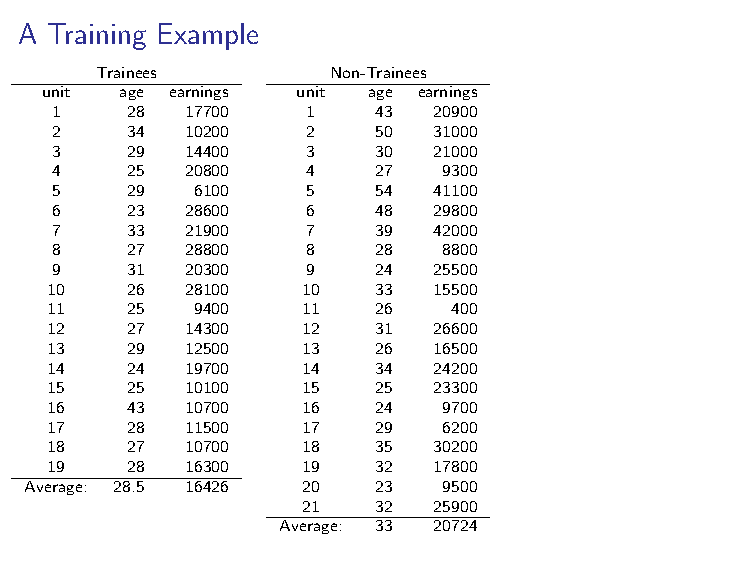
\includepdf[pages=1-last]{./lecture_includes/abadie-matching2.pdf}
%}



\begin{frame}{Measuring the matching discrepancy}

\begin{itemize}
\item What does it mean to be close when I am working with a large number of covariates?
\item What if we had a way of measuring a match in terms of how ``close'' each unit's $X_i$ value was to the matched $X_j$
\item Let's do that and use the square root of the sum of all squared differences in each unit's $X_i - X_{j(i)}$ as a measure of how bad the match is
\item This is called the Euclidean distance
\end{itemize}


\end{frame}

%\begin{frame}{Alternative distance metric: Euclidean distance}
	
% When the vector of matching covariates, $X= \colvec{X_1\\X_2\\\vdots\\X_k}$ has more than one dimension ($k>1$) we will need a new definition of \textbf{distance} to measure ``closeness''.  
%\end{frame}

\begin{frame}{Euclidean distance}
	\begin{block}{Definition: Euclidean distance}
    \vspace*{-2.5mm}
    \begin{eqnarray*}
    ||X_i-X_j|| &=& \sqrt{ (X_i-X_j)'(X_i-X_j) } \\
    &=& \sqrt{ \sum_{n=1}^k (X_{ni} - X_{nj})^2 }
    \end{eqnarray*}
    \vspace*{-2.5mm}
	\end{block}
	
Let's do this together -- sometimes it helps to manually calculate this

\bigskip

\url{https://docs.google.com/spreadsheets/d/1iro1Qzrr1eLDY_LJVzOYvnQZWmxY8JyTcDf6YcdhkwQ/edit?usp=sharing}

	
\end{frame}


%\begin{frame}{Inexact matching: Random match 1}

%\begin{figure}[!t]\centering
%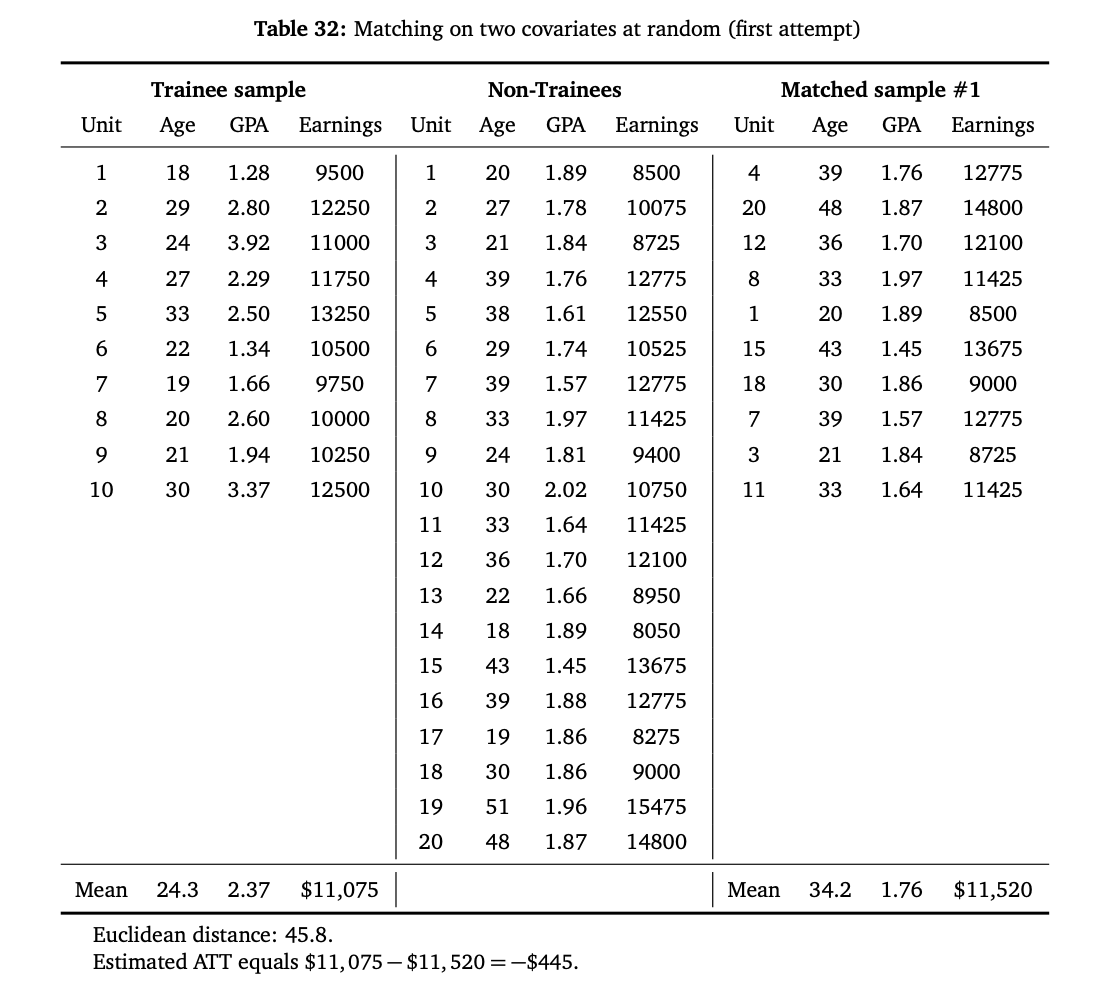
\includegraphics[scale=0.45]{./lecture_includes/inexact_random1}
%\end{figure}

%\end{frame}


%\begin{frame}{Inexact matching: Random match 2}

%\begin{figure}[!t]\centering
%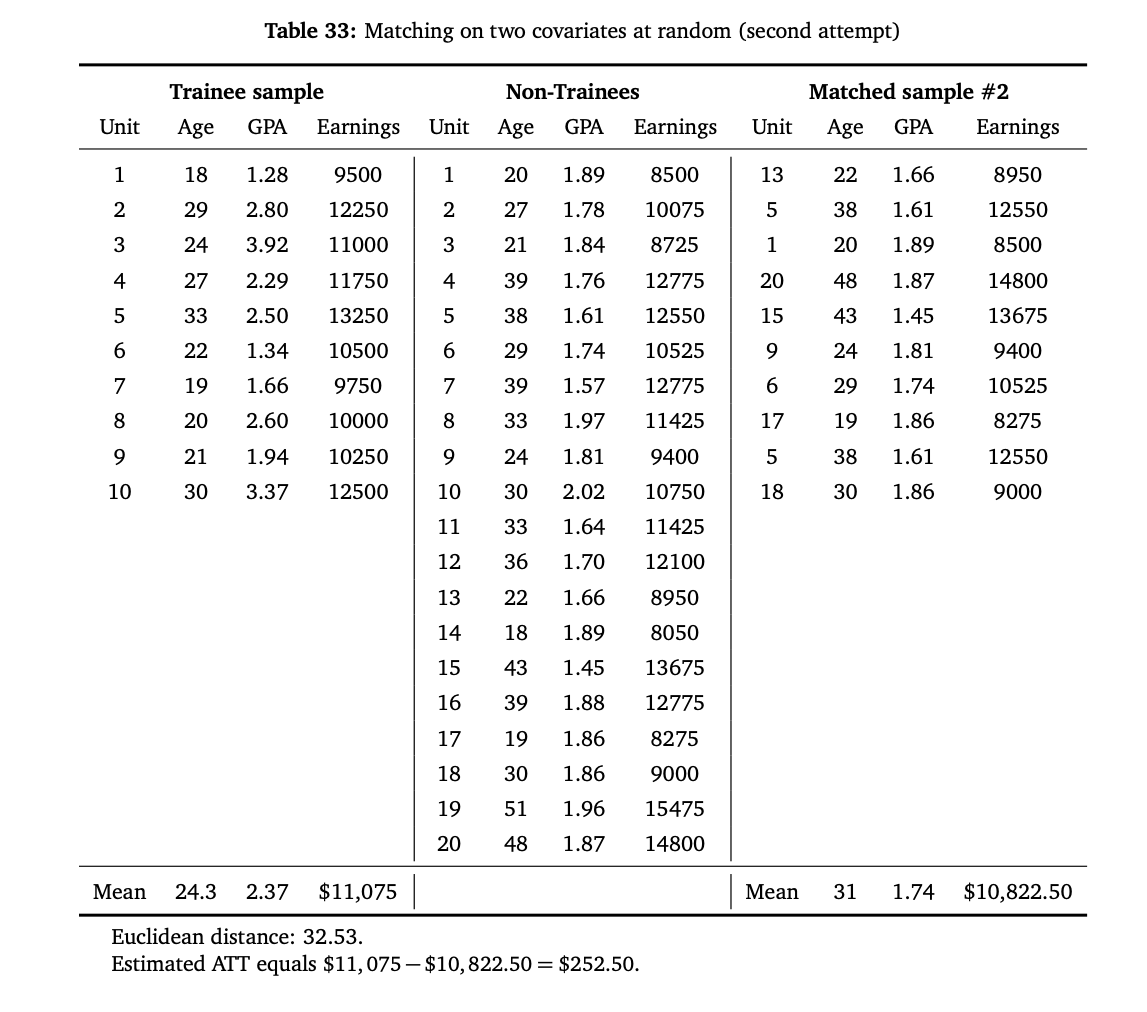
\includegraphics[scale=0.45]{./lecture_includes/inexact_random2}
%\end{figure}

%\end{frame}


\begin{frame}{Minimizing the Euclidean distance}

\begin{itemize}
\item We are minimizing Euclidean distance, and if that is not zero, then there is matching discreprancy
\item And since it is a minimum, any other match will have more matching discreprancies
\item \texttt{Matching} in R and \texttt{teffects} in Stata (not sure in python)
\end{itemize}

\end{frame}


\begin{frame}{Visualization of Optimal Match}

\begin{figure}[!t]\centering
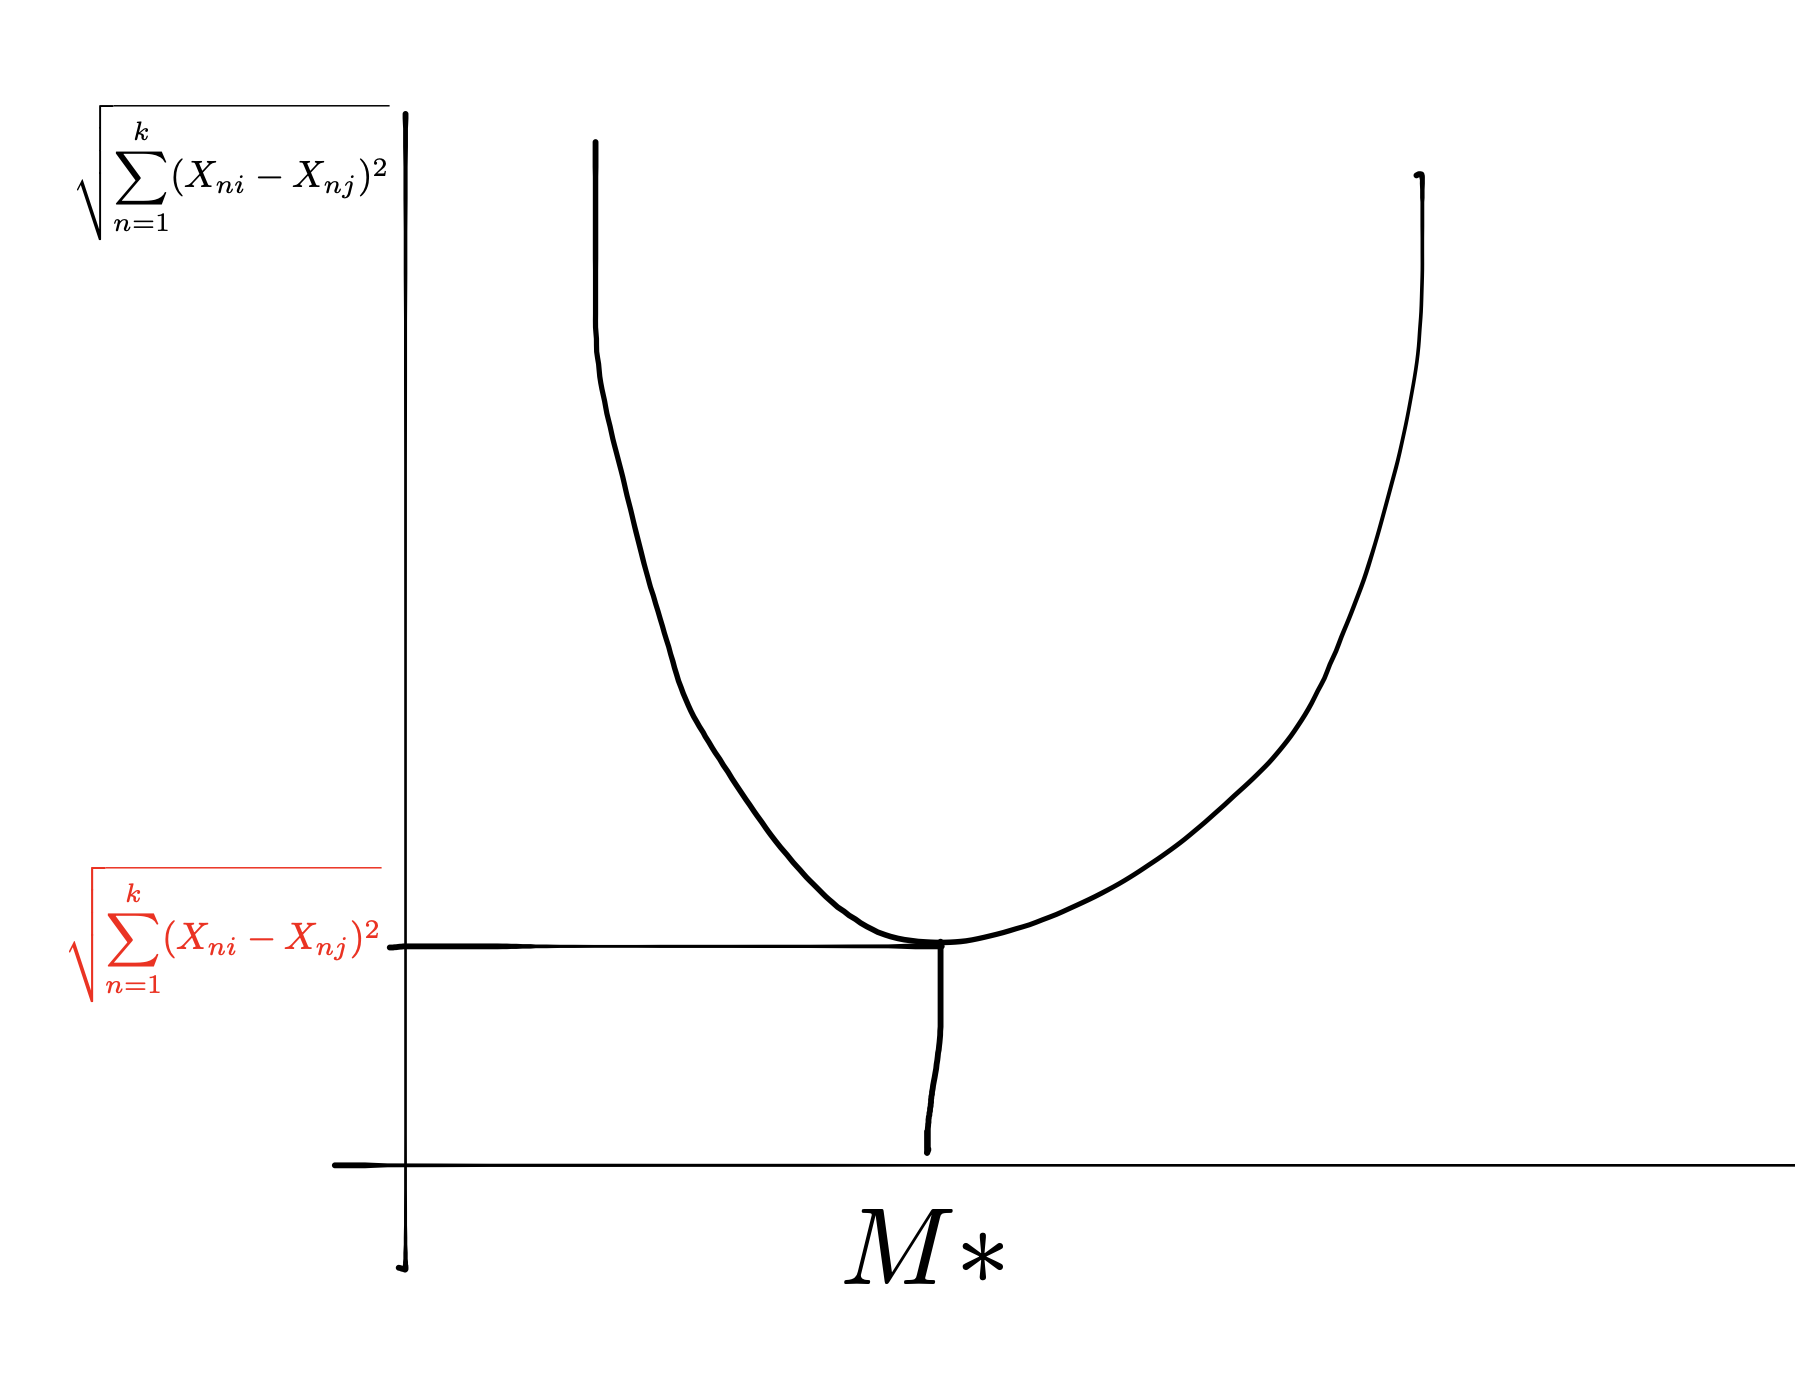
\includegraphics[scale=0.35]{./lecture_includes/optimal_matches}
\end{figure}

\end{frame}


 

%\begin{frame}{Inexact matching by minimizing the Euclidean distance}

%\begin{figure}[!t]\centering
%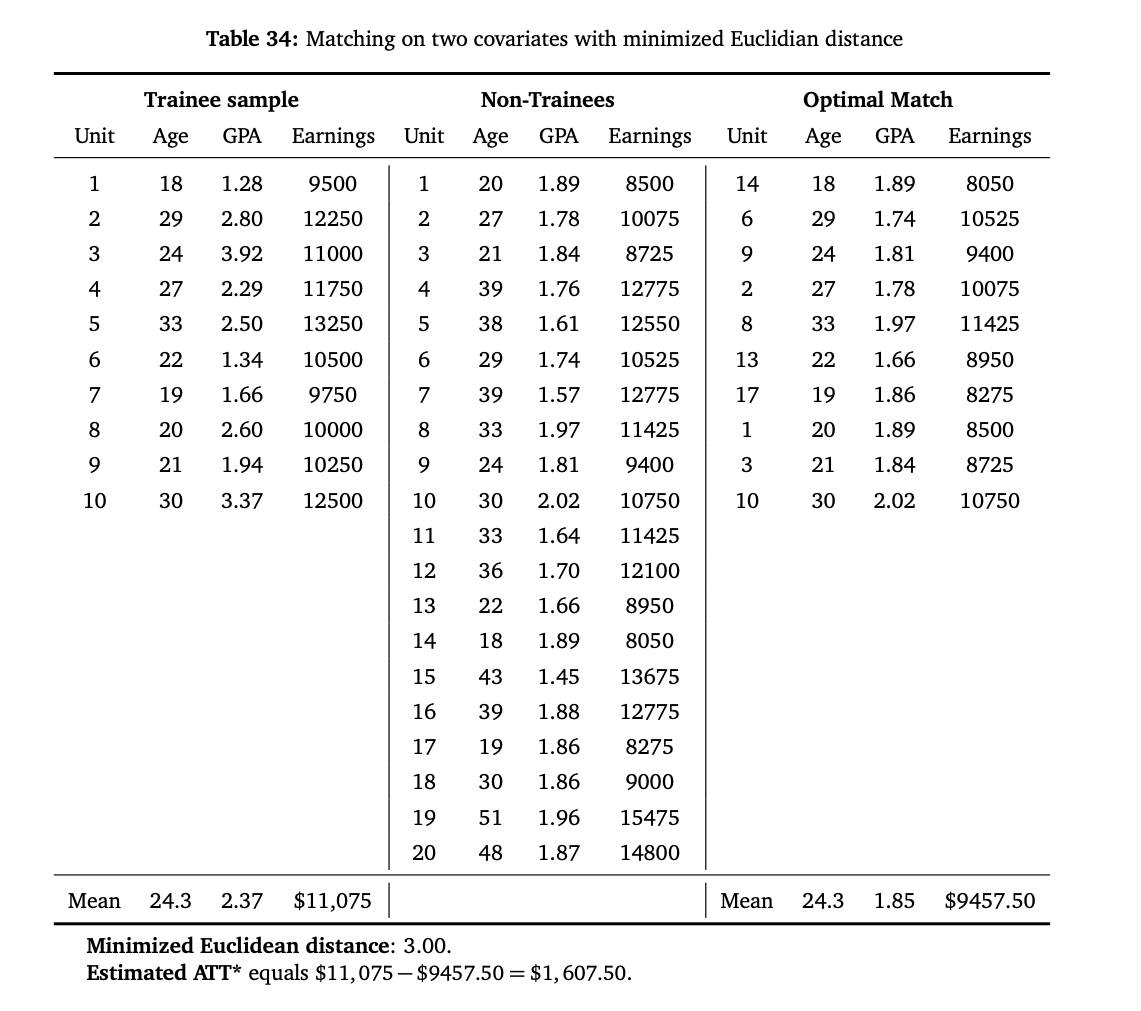
\includegraphics[scale=0.45]{./lecture_includes/inexact_euclidean}
%\end{figure}

%\end{frame}

\begin{frame}{Other distance metrics}

\begin{itemize}
\item Our example treated a one unit difference in age and one unit difference in GPA as the same, but those scales are different and matter a lot
\item The Euclidean distance is not invariant to changes in the scale of the $X$'s.  
\item Alternative distance metrics that \emph{are} invariant to changes in scale are more commonly used 
\item Normalized Euclidean distance and Mahalanobis distance both try to normalize it so that scale doesn't matter
\end{itemize}

\end{frame}


\begin{frame}{Normalized Euclidean distance}

	\begin{block}{Definition: Normalized Euclidean distance}
	  A commonly used distance is the normalized Euclidean distance:$$||X_i-X_j|| = \sqrt{ (X_i-X_j)'\widehat{V}^{-1}(X_i - X_j) }$$ where
		$$\widehat{V}^{-1} = \text{diag}(\widehat{\sigma}_1^2, \widehat{\sigma}_2^2, \dots, \widehat{\sigma}_k^2)$$
	\end{block}
\end{frame}

\begin{frame}{Normalized Euclidean distance}
	\begin{itemize}
	\item Notice that the normalized Euclidean distance is equal to:
		\begin{eqnarray*}
		||X_i - X_j|| = \sqrt{\sum_{n=1}^k \frac{(X_{ni} - X_{nj})^2}{\widehat{\sigma}^2_n}}
		\end{eqnarray*}
	\item Thus, if there are changes in the scale of $X_{ni}$, these changes also affect $\widehat{\sigma}^2_n$, and the normalized Euclidean distance does not change
	\end{itemize}

\end{frame}


\begin{frame}{Mahalanobis distance}
	
	\begin{block}{Definition: Mahalanobis distance}
	The Mahalanobis distance is the scale-invariant distance metric:
		\begin{eqnarray*}
		||X_i-X_j|| = \sqrt{ (X_i-X_j)'\widehat{\Sigma}_X^{-1}(X_i - X_j) }
		\end{eqnarray*}
	where $\widehat{\Sigma}_X$ is the sample variance-covariance matrix of $X$.
	\end{block}


\end{frame}



\begin{frame}{Matching and the Curse of Dimensionality}
	
\begin{itemize}
\item The larger the dimensions of the conditioning set, the less likely common support holds, and you can't not do it because you need these covariate dimensions to satisfy weak unconfoundedness!
\item This problem is caused by the finite dataset, and it introduces a particular type of selection bias
\item Curses are only overcome with new spells  
\item Abadie and Imbens (2011) derived a bias adjustment based on the unconfoundedness assumption and an outcome regression model
\end{itemize}

\end{frame}


\begin{frame}{Deriving the matching bias}
	
  \vspace{-5mm}
  $$
		\widehat{\delta}_{ATT} = \frac{1}{N_T} \sum_{D_i=1} (Y_i - Y_{j(i)}),
  $$
  where each $i$ and $j(i)$ units are matched, $X_i \approx X_{j(i)}$ and $D_{j(i)}=0$. 
	 
  \bigskip
  Define potential outcomes and switching eq.
		\begin{eqnarray*}
      \mu^0(x) &=& E[Y | X=x,D=0] = E[Y^0 | X=x],\\
      \mu^1(x) &=& E[Y | X=x,D=1] = E[Y^1 | X=x],\\
      Y_i &=& \mu^{D_i}(X_i) + \varepsilon_i
		\end{eqnarray*}
\end{frame}

\begin{frame}{Deriving the matching bias}
  Substitute and distribute terms
  \begin{eqnarray*}
    \widehat{\delta}_{ATT} &=& \frac{1}{N_T} \sum_{D_i=1} (Y_i - Y_{j(i)}) \\
    &=& \frac{1}{N_T} \sum_{D_i=1} \left[ (\mu^1(X_i) + \varepsilon_i) - (\mu^0(X_{j(i)}) + \varepsilon_{j(i)}) \right] \\
    &=&  \frac{1}{N_T} \sum_{D_i=1} (\mu^1(X_i) - \mu^0(X_{j(i)})) + \frac{1}{N_T} \sum_{D_i=1}(\varepsilon_i - \varepsilon_{j(i)})
  \end{eqnarray*}
\end{frame}
		

\begin{frame}{Deriving the matching bias}
	
Difference between sample estimate and population parameter is:
		\begin{eqnarray*}
		\widehat{\delta}_{ATT} - \delta_{ATT} &=& \frac{1}{N_T} \sum_{D_i=1} \left( \mu^1(X_i) - \mu^0(X_{j(i)}) - \delta_{ATT}\right) \\
		&+& \frac{1}{N_T} \sum_{D_i=1} (\varepsilon_i - \varepsilon_{j(i)})
		\end{eqnarray*}
Algebraic manipulation and simplification:
		\begin{eqnarray*}
		\widehat{\delta}_{ATT} - \delta_{ATT} &=& \frac{1}{N_T} \sum_{D_i=1} \left( \mu^1(X_i) - \mu^0(X_i) - \delta_{ATT}\right) \\
		&+& \frac{1}{N_T} \sum_{D_i=1} (\varepsilon_i - \varepsilon_{j(i)}) \\
		&+& \frac{1}{N_T} \sum_{D_i=1} \left( \mu^0(X_i) - \mu^0(X_{j(i)}) \right).
		\end{eqnarray*}
\end{frame}


\begin{frame}{Deriving the matching bias}
	
Note $\widehat{\delta}_{ATT} - \delta_{ATT} \to 0$ as $N \to \infty$.
\pause However, 
$$E[ \sqrt{\frac{1}{N}} (\widehat{\delta}_{ATT} - \delta_{ATT})] = E[ \sqrt{\frac{1}{N}} ( \mu^0(X_i) - \mu^0(X_{j(i)}) ) | D=1].$$ 
\pause
Now consider the implications if $k$ is large:
\pause	\begin{itemize}
	\item The difference between $X_i$ and $X_{j(i)}$ converges to zero very slowly 
\pause	\item The difference $\mu^0(X_i) - \mu^0(X_{j(i)})$ converges to zero very slowly \pause
	\item $E[ \sqrt{\frac{1}{N}} (\mu^0(X_i) - \mu^0(X_{j(i)})) | D=1]$ may not converge to zero and an be very large! 
\pause	\item $E[ \sqrt{\frac{1}{N}} (\widehat{\delta}_{ATT} - \delta_{ATT})]$ may not converge to zero because the bias of the matching discrepancy is dominating the matching estimator! \pause
	\end{itemize}
 Bias is often an issue when we match in many dimensions
\end{frame}

\begin{frame}{Solutions to matching bias problem}
	
The bias of the matching estimator is caused by large matching discrepancies $||X_i - X_{j(i)}||$ which is virtually guaranteed by the curse of dimensionality.  However:
	\begin{enumerate}
	\item But the matching discrepancies are observed. We can always check in the data how well we're matching the covariates.

	\item For $\widehat{\delta}_{ATT}$ we can sometimes make the matching discrepancies small by using a large reservoir of untreated units to select the matches (that is, by making $N_C$ large).

  \item If the matching discrepancies are large, so we are worried about potential biases, we can apply bias correction techniques

	\end{enumerate}
\end{frame}

 
\begin{frame}{Matching with bias correction}
	
	\begin{itemize}
	\item Each treated observation contributes$$\alert{\mu^0(X_i)} - \mu^0(X_{j(i)})$$to the bias.
	\item Bias-corrected (BC) matching:
		\begin{eqnarray*}
		\widehat{\delta}_{ATT}^{BC} = \frac{1}{N_T} \sum_{D_i=1} \left[ (Y_i - Y_{j(i)}) - ( \widehat{\mu^0}(X_i) - \widehat{\mu^0}(X_{j(i)}) ) \right]
		\end{eqnarray*}where $\widehat{\mu^0}(X)$ is an estimate of $E[Y|X=x,D=0]$.  For example using OLS but other maybe too (neural nets?).  
	\item Under some conditions, the bias correction eliminates the bias of the matching estimator without affecting the estimator's variance.
	\end{itemize}
\end{frame}

\begin{frame}{Intuition}

\begin{itemize}
\item Under unconfoundedness, we know that $$\textcolor{red}{E[Y^0|D=1, X=x]} = E[Y^0|D=0, X=x]$$
\item This implies that whatever the relationship is between $Y^0$ and $X$ in the control group, it's the same in the treatment group, even though we cannot observe $Y^0$ in the treatment group
\item We will therefore fit a regression of $Y^0$ onto $X$ in the $D=0$ group only and use that to predict $\widehat{Y^0}$ in both groups
\end{itemize}

\end{frame}


\begin{frame}{Steps}

\begin{enumerate}
\item[1.  ]Regress $Y$ on $X$ with OLS except only use the control sample:
\begin{equation}
Y^0_j = \alpha + \beta X_j + \varepsilon_j \nonumber
\end{equation}where $j$ are the units for which $D_j=0$.  
\end{enumerate}

\end{frame}

\begin{frame}{Steps}

\begin{enumerate}
\item[2. ] Use the fitted values $\widehat{\alpha}$ and $\widehat{\beta}$ to predict $\widehat{\mu}^0(X)$ for both the $i$ and the matched $j(i)$ units:
\begin{eqnarray}
\widehat{\mu}^0_i &=& \widehat{\alpha} + \widehat{\beta} X_i \nonumber \\
\widehat{\mu}^0_{j(i)} &=& \widehat{\alpha} + \widehat{\beta} X_{j(i)} \nonumber
\end{eqnarray}
\end{enumerate}

\end{frame}


\begin{frame}{Steps}

\begin{enumerate}
\item[3. ] Subtract $ \widehat{\mu}_i^0(X_i) - \widehat{\mu}_{j(i)}^0(X_{j(i)})$, our estimate of the selection bias caused by matching discrepancies, from the sample estimate of the $ATT$: $$\widehat{\delta}_{ATT}^{BC} = \dfrac{1}{N_T} \sum_{D_i=1} \bigg [ (Y_i - Y_{j(i)}) - \Big(\widehat{\mu}^0(X_i) - \widehat{\mu}^0(X_{j(i)})\Big) \bigg ]$$
\end{enumerate}

\end{frame}


\begin{frame}{Steps}

\begin{enumerate}
\item[4. ] Estimate Abadie-Imbens robust standard error (Abadie and Imbens 2006; 2008; 2011)
\end{enumerate}

\end{frame}



\begin{frame}[plain,shrink=0]
	\begin{center}
	\textbf{Bias adjustment in matched data}
	\end{center}
	
	\begin{table}
	\begin{tabular}{c|c|c|c|c}
	\hline
	\multicolumn{1}{c}{}&
	\multicolumn{2}{c}{Potential Outcome}&
	\multicolumn{1}{c}{}&
	\multicolumn{1}{c}{}\\
	\multicolumn{1}{c}{unit} &
	\multicolumn{1}{c}{under Treatment}&
	\multicolumn{1}{c}{under Control}&
	\multicolumn{1}{c}{}&
	\multicolumn{1}{c}{}\\
	\hline
	$i$ & $Y^1_i$ & $Y^0_i$ & $D_i$ & $X_i$ \\
	\hline
	1 & \textcolor{blue}{10} &  \textcolor{blue}{8} & 1 & \textcolor{blue}{3} \\
	2 & 4 &  			 1 &				 1 & 1 \\
	3 & \textcolor{green}{10} &   \textcolor{green}{9} & 1 & \textcolor{green}{10} \\
	\hline
	4 &  & \textcolor{blue}{8} & 0 & \textcolor{green}{4} \\
	5 &  & 			 1 & 0 &  				0 \\
	6 &  & \textcolor{green}{9} & 0 & \textcolor{green}{8} \\
	\hline
	\end{tabular}
	\end{table}
	
	
	\begin{flalign*}
		\only<1-3>{&\widehat{\delta}_{ATT} = \frac{10-8}{3} + \frac{4-1}{3}  + \frac{10-9}{3}  = 2&} \\
		\only<2-3>{&\text{For the bias correction, estimate }\widehat{\mu^0}(X) = \widehat{\beta_0} + \widehat{\beta_1}X = 2+X}\\
		\only<3-3>{&\widehat{\delta}_{ATT} = \frac{ (10-8) - ( \widehat{\mu^0}(3) - \widehat{\mu^0}(4)) }{3}  + \frac{ (4-1)  -( \widehat{\mu^0}(1) - \widehat{\mu^0}(0)) }{3}  \\
		&+ \frac{ (10-9)  - ( \widehat{\mu^0}(10) - \widehat{\mu^0}(8))}{3} = 1.33}
	\end{flalign*}

\end{frame}


\begin{frame}{Matching bias: Implications for practice}
	
\emph{Matching} bias arises because of the effect of large matching discrepancies on $\mu^0(X_i) - \mu^0(X_{j(i)})$ due to a lack of common support. To minimize matching discrepancies:
	\begin{enumerate}
	\item Use a small $M$ (e.g., $M=1$). Larger values of $M$ produce large matching discrepancies.
	\item Use matching with replacement.  Because matching with replacement can use untreated units as a match more than once, matching with replacement produces smaller matching discrepancies than matching without replacement.
	\item Try to match covariates with a large effect on $\mu^0(\cdot)$ particularly well.
	\end{enumerate}
\end{frame}

\begin{frame}{Large sample distribution for matching estimators}
	
	\begin{itemize}
	\item Cannot use the bootstrap, so Abadie and Imbens derived the variance (Abadie and Imbens 2008)
	\item Matching estimators have a Normal distribution in large samples (provided the bias is small):
		\begin{eqnarray*}
		\sqrt{N_T} (\widehat{\delta}_{ATT} - \delta_{ATT}) \xrightarrow{d} N(0,\sigma^2_{ATT})
		\end{eqnarray*}
	\item For matching without replacement, the ``usual'' variance estimator:
		\begin{eqnarray*}
		\widehat{\sigma}^2_{ATT} = \frac{1}{N_T} \sum_{D_i=1} \left( Y_i - \frac{1}{M} \sum_{m=1}^M Y_{j_m(i)} - \widehat{\delta}_{ATT} \right)^2,
		\end{eqnarray*}is valid.
	\end{itemize}
\end{frame}

\begin{frame}{Large sample distribution for matching estimators}
	
	\begin{itemize}
	\item For matching with replacement:
		\begin{eqnarray*}
		\widehat{\sigma}^2_{ATT} &=& \frac{1}{N_T} \sum_{D_i=1} \left( Y_i - \frac{1}{M} \sum_{m=1}^M Y_{j_m(i)} - \widehat{\delta}_{ATT} \right)^2 \\
		&+& \frac{1}{N_T} \sum_{D_i=0} \left( \frac{K_i(K_i-1)}{M^2} \right) \widehat{var}(\varepsilon | X_i,D_i=0)
		\end{eqnarray*}where $K_i$ is the number of times observation $i$ is used as a match.
	\item $\widehat{var}(Y_i | X_i,D_i=0)$ can be estimated also by matching.  For example, take two observations with $D_i=D_j=0$ and $X_i \approx X_j$, then
		\begin{eqnarray*}
		\widehat{var}(Y_i | X_i,D_i=0) = \frac{(Y_i-Y_j)^2}{2}
		\end{eqnarray*}is an unbiased estimator of $\widehat{var}(\varepsilon_i | X_i,D_i=0))$
	\end{itemize}
\end{frame}

\begin{frame}{Example}

Let's now review the syntax in Stata.  It's called \texttt{matching.do} and is in /Labs/Matching 

\bigskip

\url{https://github.com/scunning1975/Torino-2024/tree/main/Labs/Matching}

\end{frame}


\subsection{Propensity scores}


\begin{frame}{Curse of dimensionality, bias and heterogeneous treatment effects}
	
	\begin{itemize}
	\item Recall the problem of many covariates for exact matching -- the curse of dimensionality makes matching on $K$ covariates implausible as the dimensions grow exponentially with $K$ 
	\item This is problem because recall there are two assumptions needed to match
		\begin{enumerate}
		\item Unconfoundedness: this gives you the right to match
		\item Common support: this gives you the ability to match
		\end{enumerate}
	\item Without both, then depending on the amount of hetergeneity in the treatment effects, matching will be biased
	\end{itemize}

\end{frame}

\begin{frame}{Propensity score as dimension reduction}
	
	\begin{itemize}

	\item Rubin (1977) and Rosenbaum and Rubin (1983) developed the propensity score method
	\item They show that if treatment is independent of potential outcomes conditional on $K$ covariates, then it will be independent of potential outcomes conditional on propensity score 
	\item Main value of the propensity score is dimension reduction  to reduce $K$ covariates into a single scalar without loss of information
	\item Variety of ways to incorporate the propensity score -- stratification, weighting and matching
	\end{itemize}
	
\end{frame}


\begin{frame}{Investigating overlap}

\begin{itemize}

\item Once you obtain the propensity score, you can use it for estimation, but you can also use it for evaluating covariate balance
\item It's an easy way to do it with histograms, and since the propensity score theorem holds for the dimensions of $X$, there's no loss of generality in investigating overlap that way versus one by one 
\item Remember: you need common support, not on $X$ individual covariates alone, but within the $K$ dimensions, so investigating with the propensity score is easier to do

\end{itemize}

\end{frame}



\begin{frame}{Covariate 1  histograms}

  \begin{figure}
    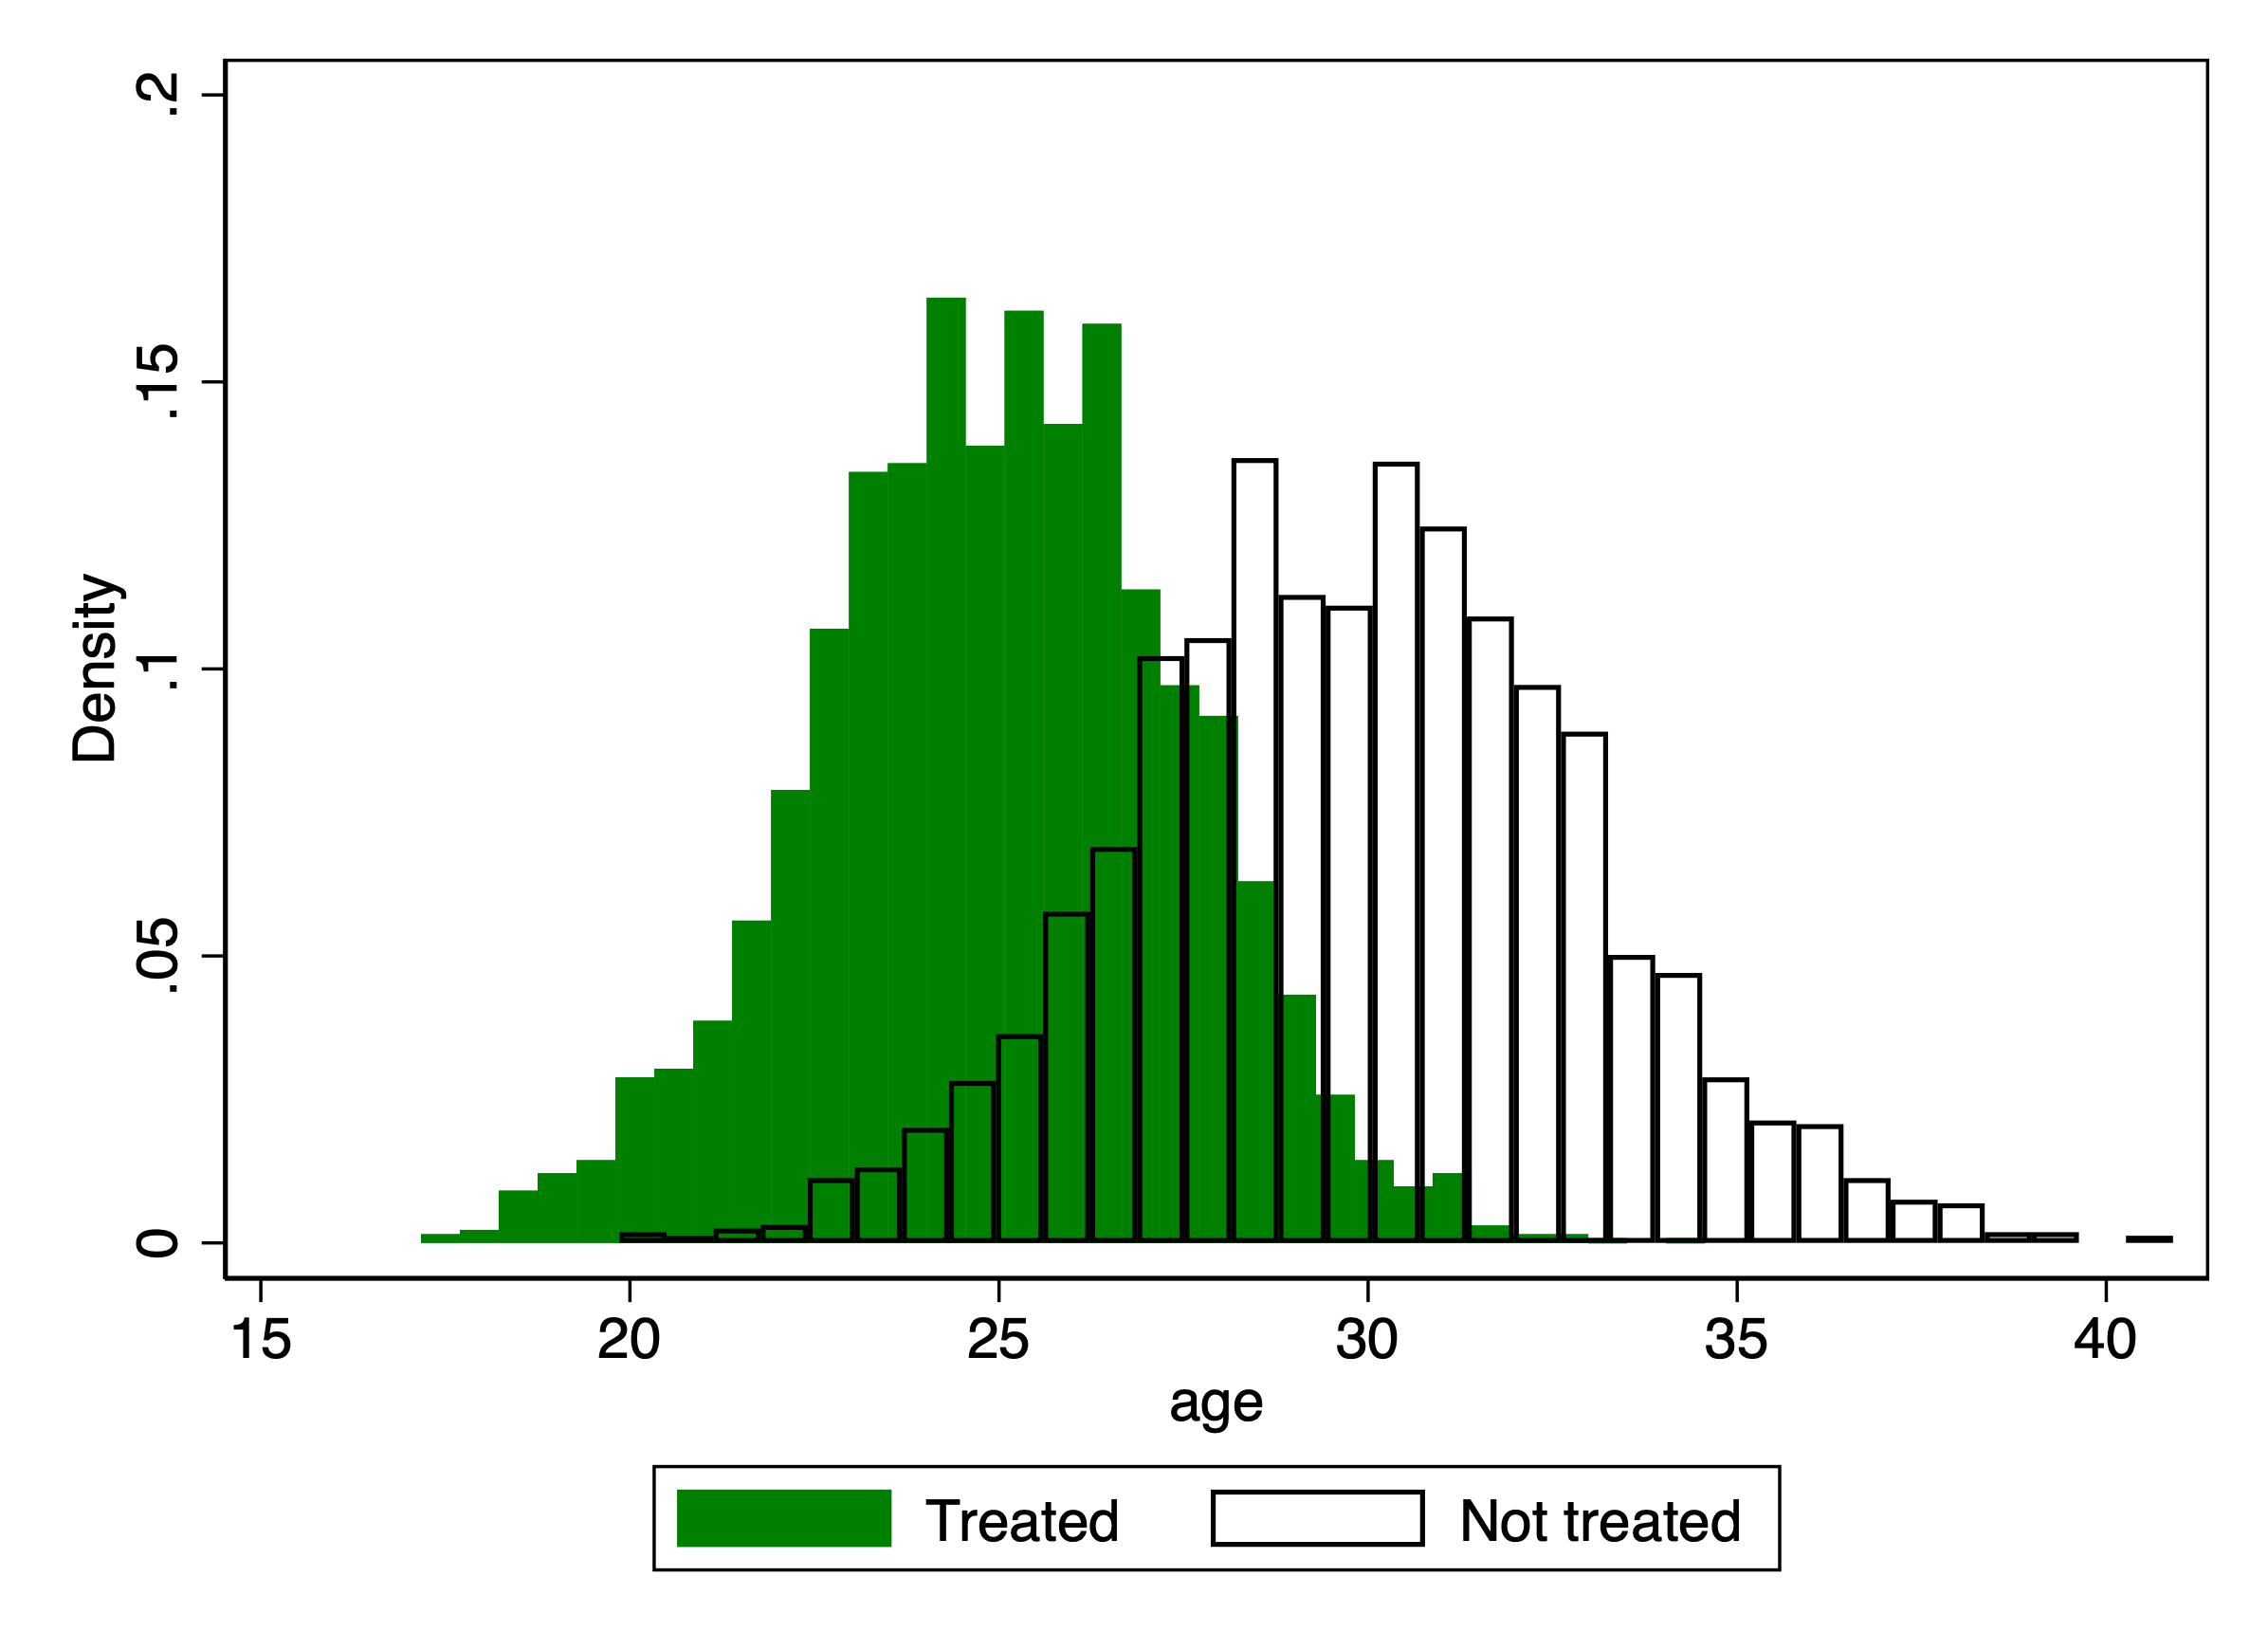
\includegraphics[scale=0.25]{./lecture_includes/age_histogram}
  \end{figure}
  
\end{frame}

\begin{frame}{Covariate 2  histograms}

  \begin{figure}
    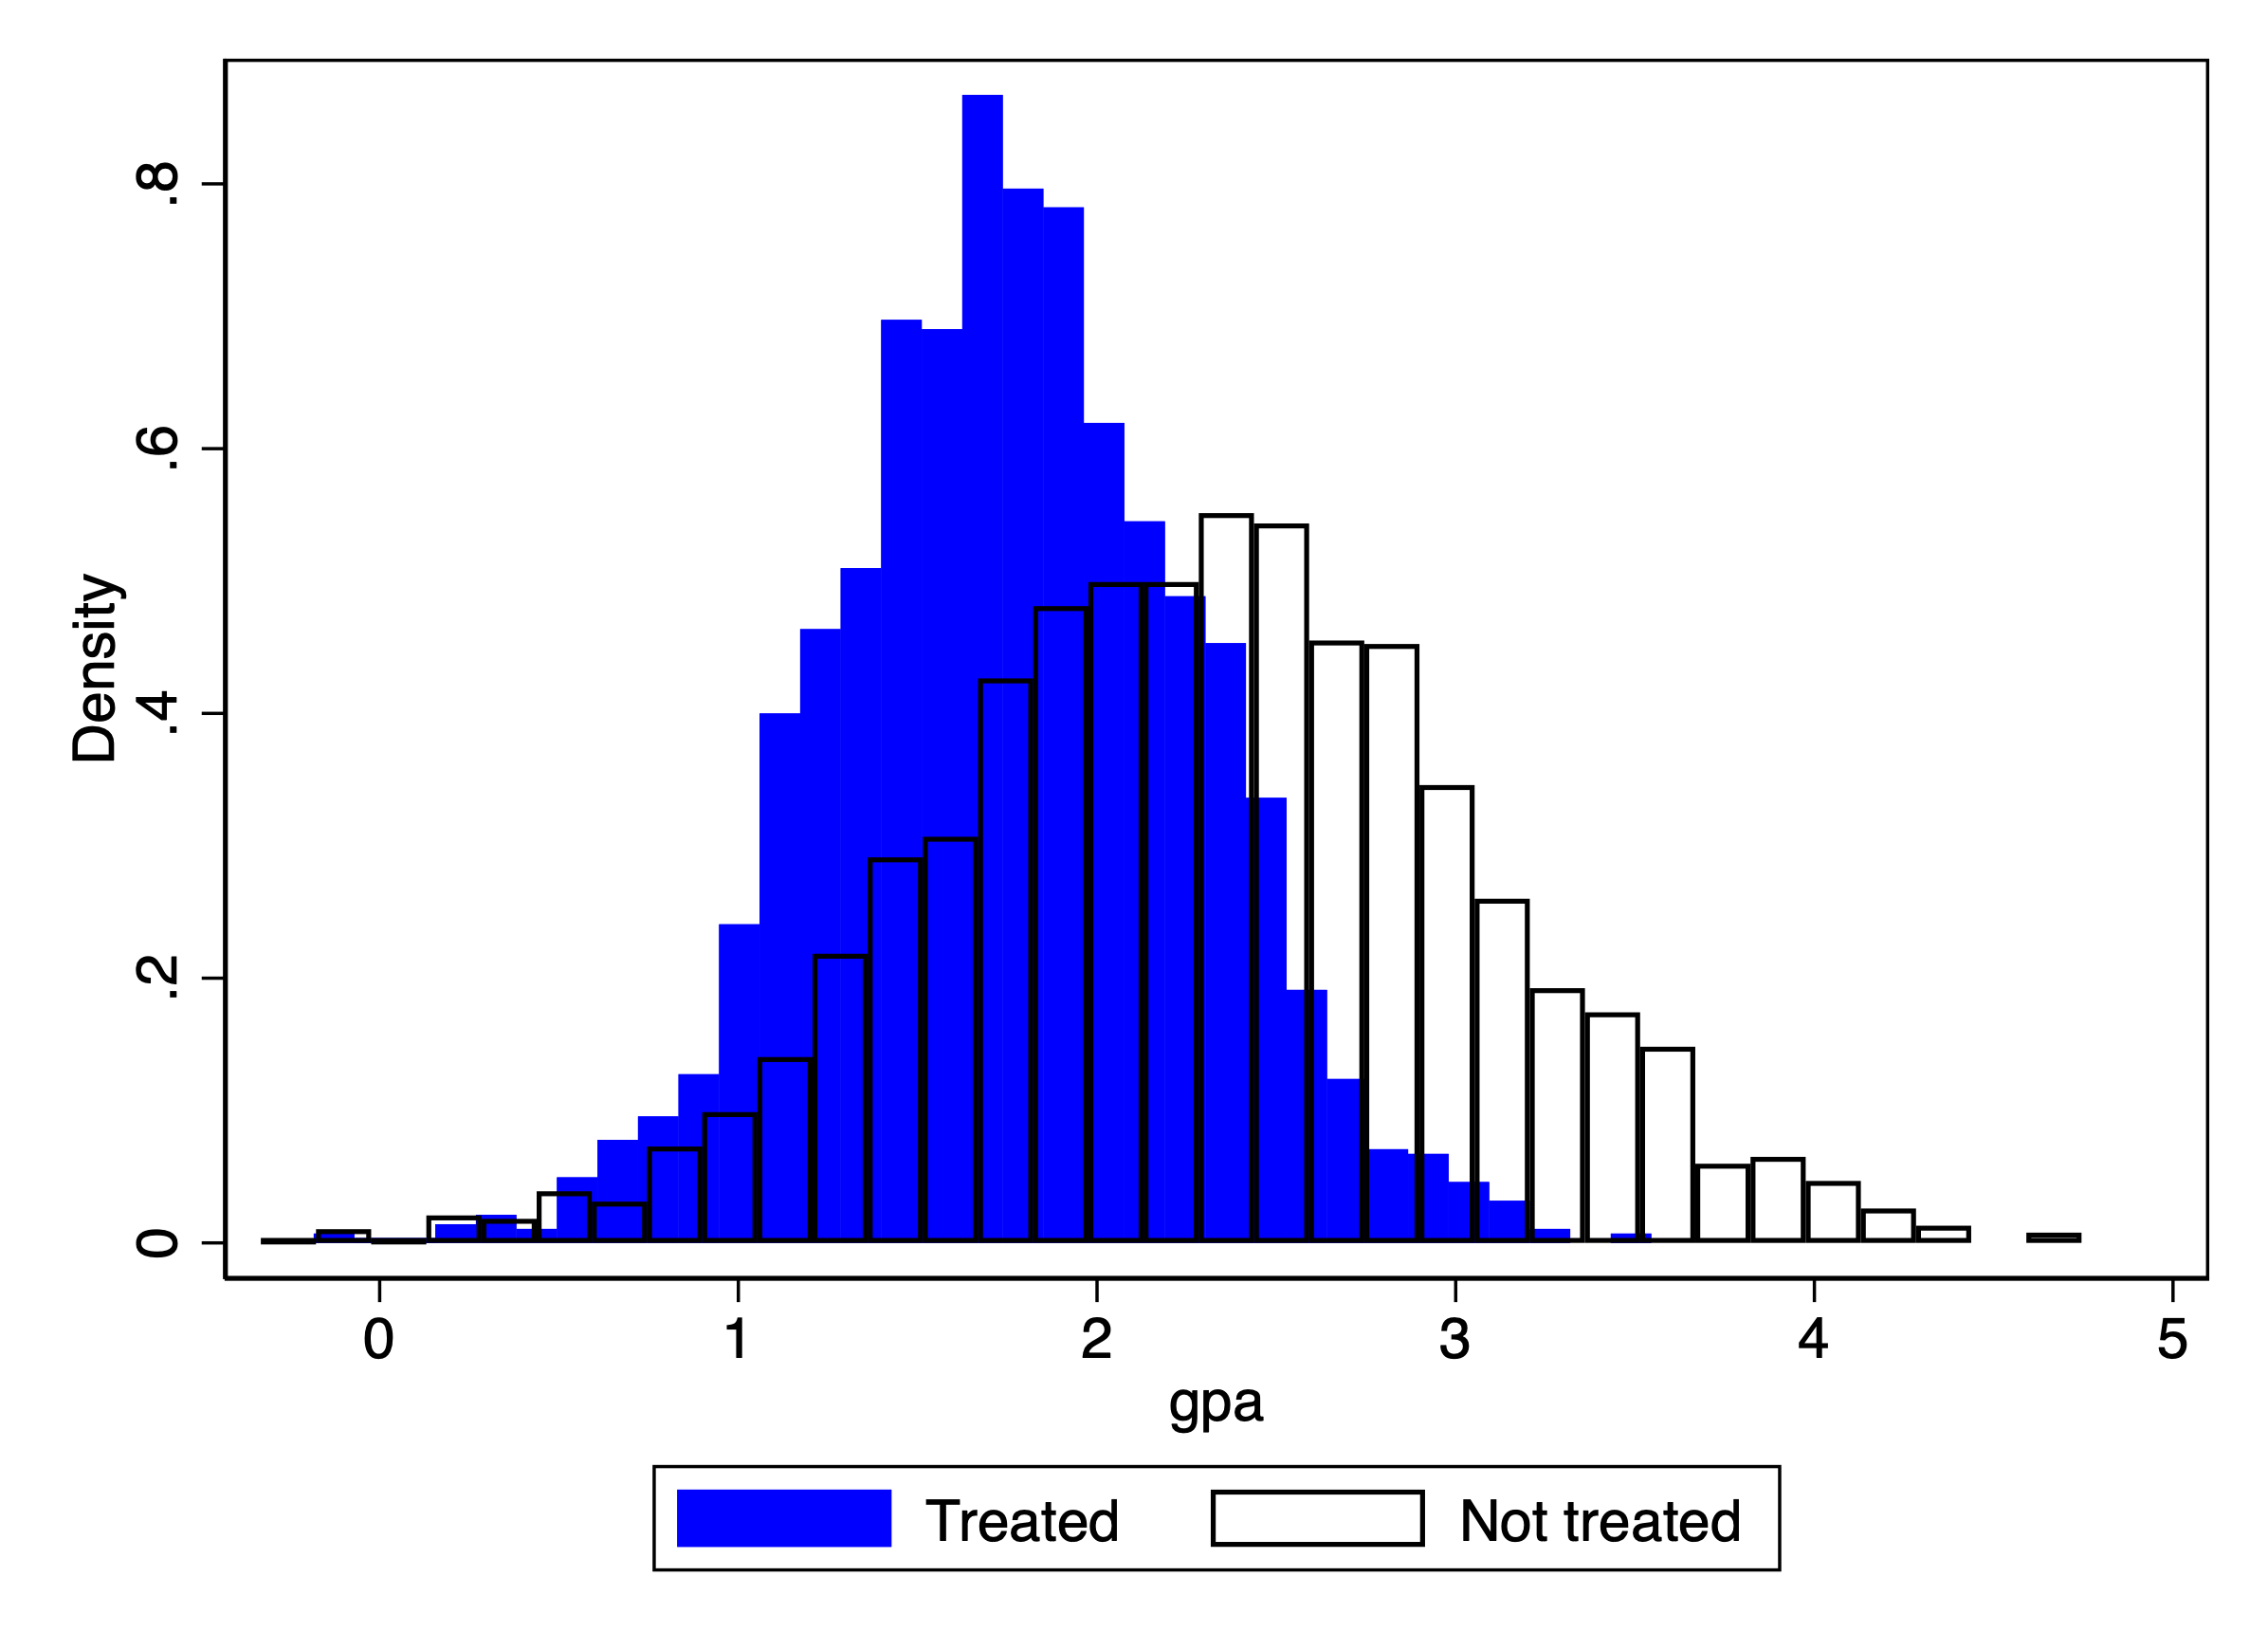
\includegraphics[scale=0.25]{./lecture_includes/gpa_histogram}
  \end{figure}
  
\end{frame}

\begin{frame}{Summarizing both with propensity score histogram}

  \begin{figure}
    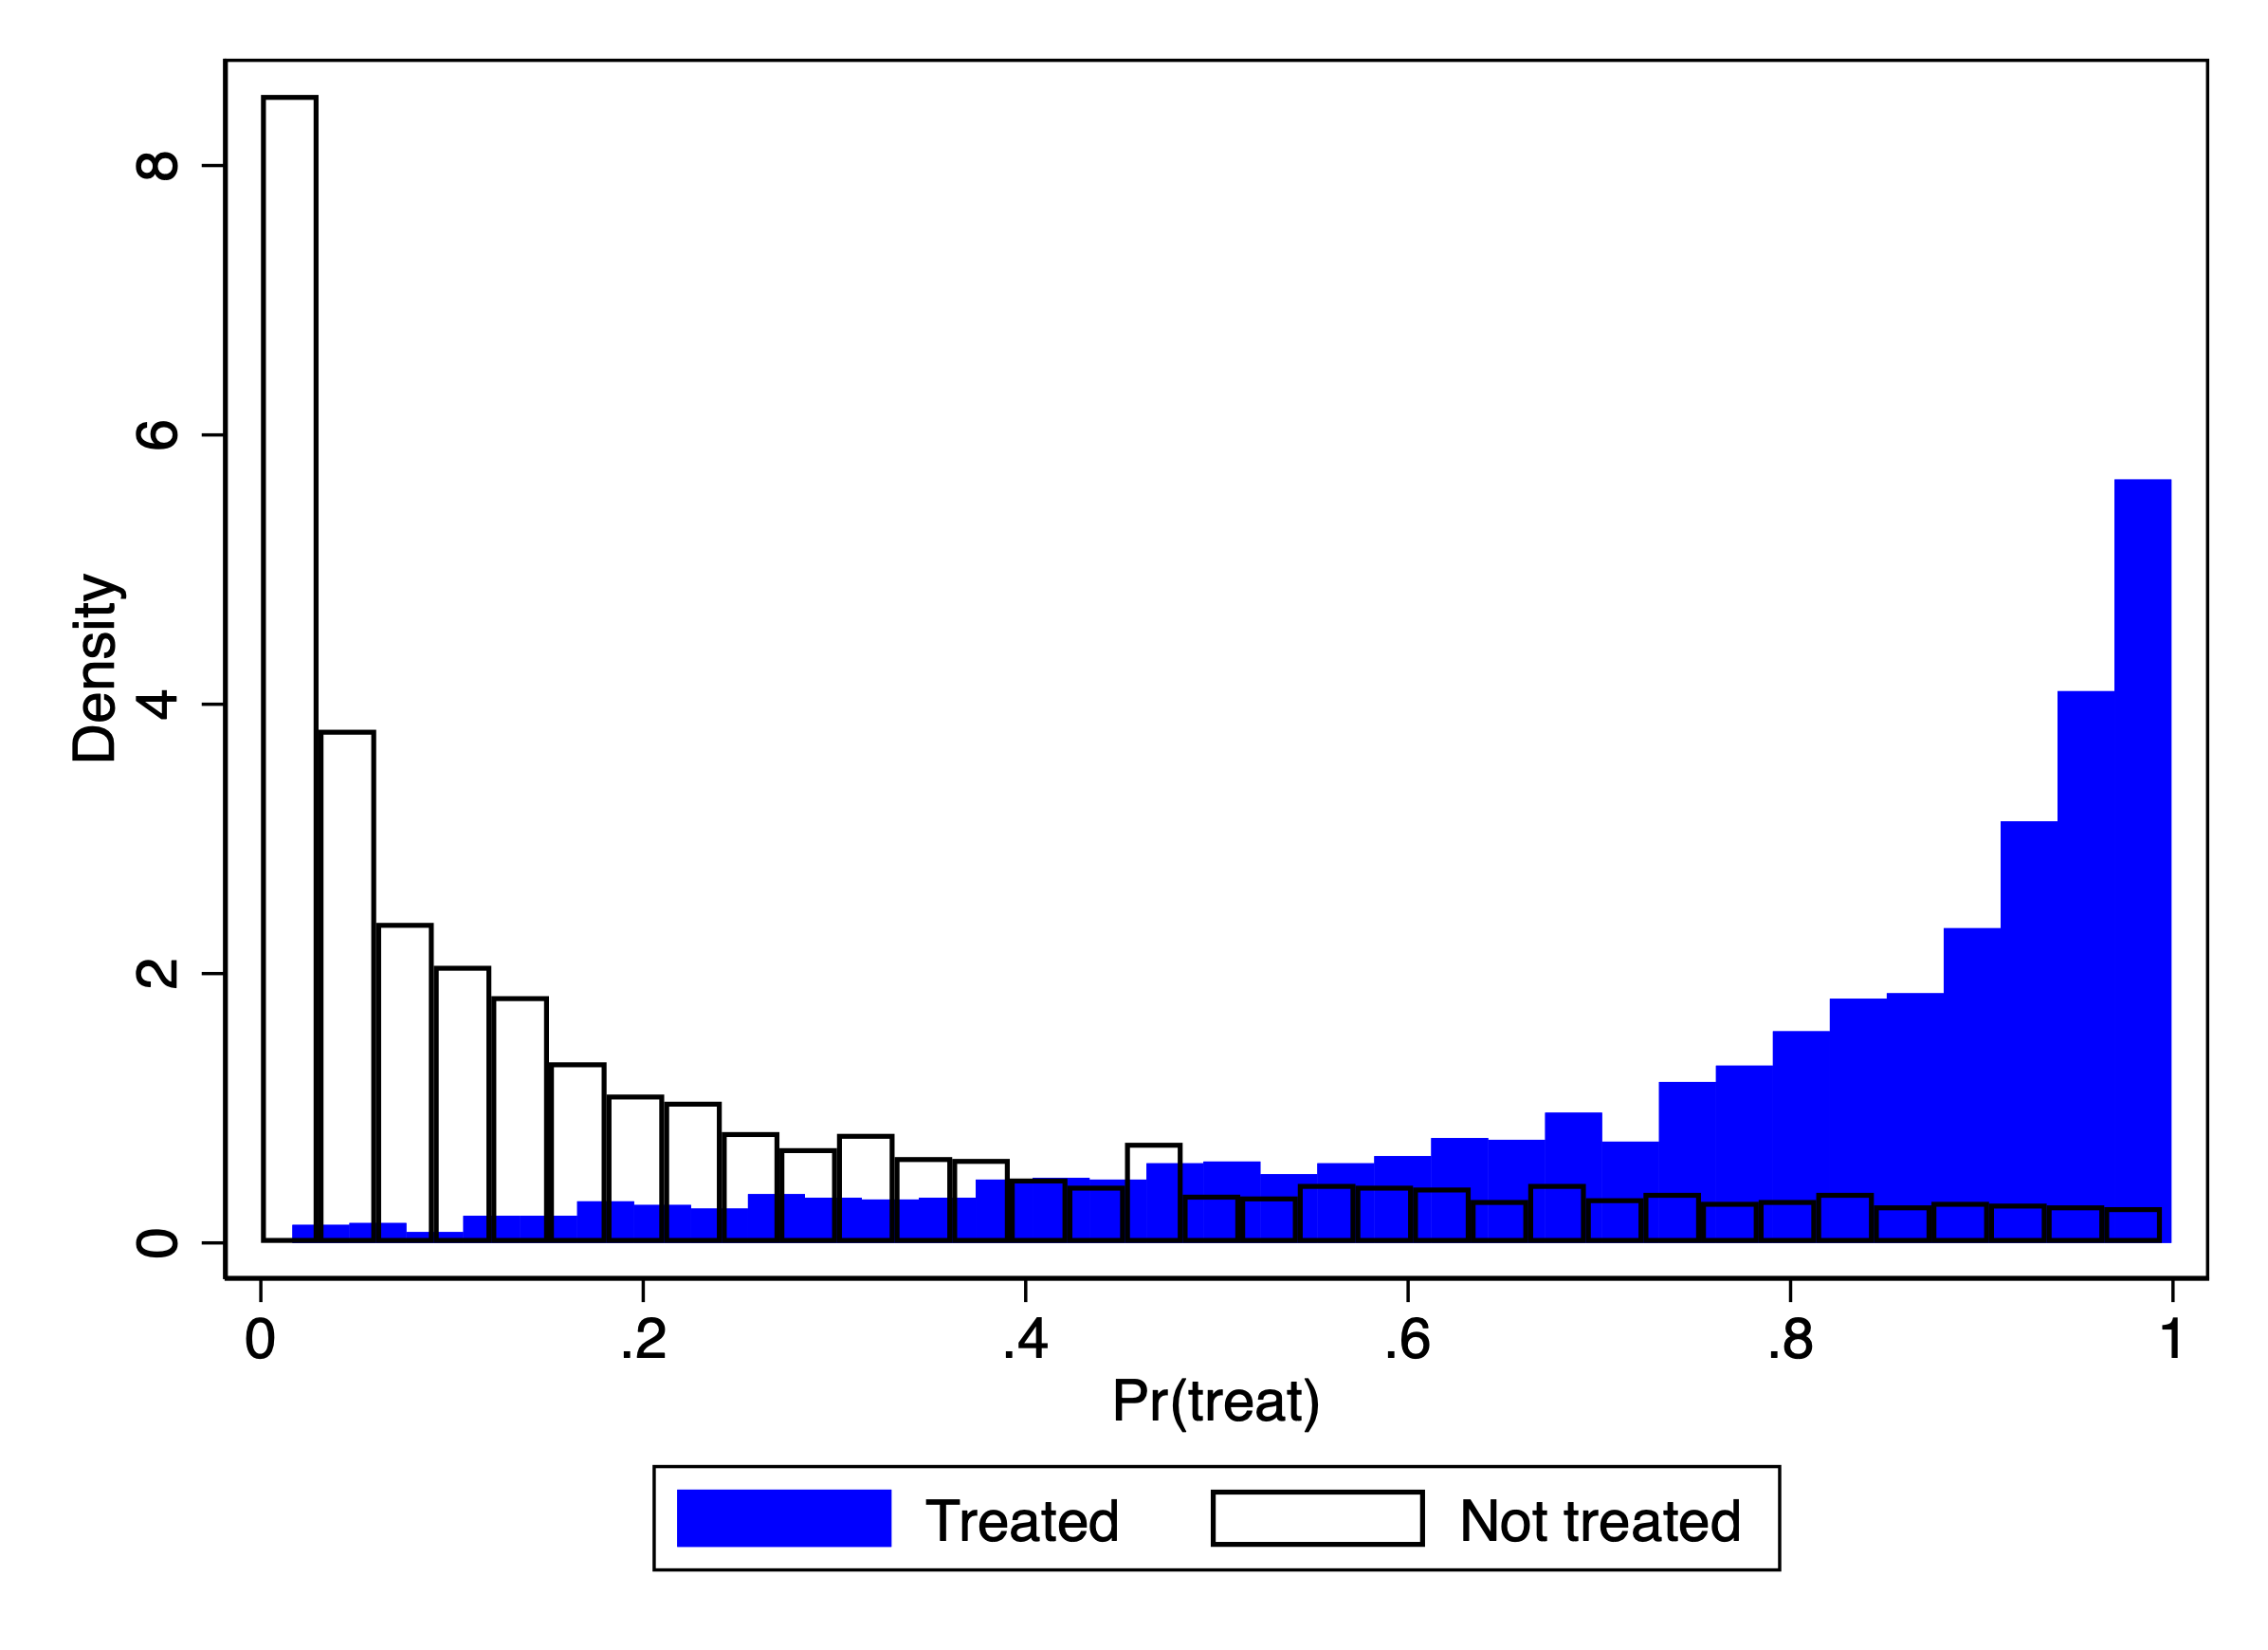
\includegraphics[scale=0.25]{./lecture_includes/pscore_histogram}
  \end{figure}
  
\end{frame}







\begin{frame}{Navigating the vastness of estimation}

\begin{itemize}
\item Estimators abound and can be a little bewildering so to summarize them:
	\begin{enumerate}
	\item Match units from one group to another using the propensity score (with various rules for finding how close to be)
	\item Weighting by the inverse propensity score
	\end{enumerate}
\item Variety of techniques to derive standard errors from parametric methods to bootstrapping
\item Can even introduce ``doubly robust'' methods to deal with matching bias like we did with nearest neighbor bias correction
\item But all these estimators assume unconfoundedness, so really it's all about addressing the lack of overlap; that's the only bias that exists when you have unconfoundedness remember
\end{itemize}

\end{frame}




\begin{frame}{Formal Definition}
	
	\begin{block}{Definition of Propensity score}
	A propensity score is a number bounded between 0 and 1 measuring the probability of treatment assignment conditional on a vector of confounding variables: $p(X)=Pr(D=1 | X)$
	\end{block}
	

\end{frame}

\begin{frame}{Propensity score theorem}

``We are interested in estimating the average effect of a binary treatment on a scaler outcome.  If assignment to the treatment is exogenous or unconfounded, that is, independent of the potential outcomes given covariates, biases associated with simple treatment-control average comparisons can be removed by adjusted for differences in the covariates.  Rosenbaum and Rubin (1983) show that adjusting solely for differences between treated and control units in the propensity score removes all biases associated with differences in covariates.'' -- Kirano, Imbens and Ridder (2003, Econometrica)

\end{frame}

\begin{frame}{Propensity score theorem}
	
	\begin{block}{Propensity score theorem}
	If $(Y^1,Y^0)\independent{D}|X$ (full unconfoundedness), then $(Y^1,Y^0)\independent{D} | \rho(X)$ where $\rho(X)=Pr(D=1|X)$, the propensity score
	\end{block}
	
	\begin{itemize}
	\item Conditioning on the propensity score is enough to have independence between $D$ and $(Y^1,Y^0)$ (Rosenbaum and Rubin 1983)
	\item With full unconfoundedness, you can estimate the ATE, but you can estimate the ATT with weaker assumptions (independence with respect to $(Y^0)\independent{D} | \rho(X)$)
	\item But remember -- propensity scores don't solve unconfoundedness; if you don't have it with respect to $K$ dimensions of $X$, you won't have it when you collapse it to the propensity score
	\end{itemize}
\end{frame}

\begin{frame}{True vs Estimating Propensity Score}


\begin{itemize}
\item Outside the randomized experiment, we don't know the ``true propensity score''
	\begin{itemize}
	\item We use DAGs or hunches to select covariates, careful not to include outcomes or colliders
	\item But we still won't know the functional form (i.e., logit, probit, polynomials, interactions)
	\end{itemize}
\item Often then people will use higher order terms and interactions to provide flexibility but it does technically have misspecification biases
\item This is an area most likely where machine learning could greatly enhance the estimation (take your pick)
\end{itemize}

\end{frame}




\begin{frame}{Step 1: Pick your parameter ATE vs ATT vs ATU}

\begin{itemize}
	\item Which population are you studying?  Only those who were discriminated against?  That's the ATT
	\item Do you want to imagine ``what if blacks and whites were both discriminated against?'' That's the ATE
	\item The more you can focus on one particular causal parameter, the easier and more justified it gets as it weakens both assumptions
\end{itemize}

\end{frame}


\begin{frame}{Step 2: Estimate the propensity score}

		\begin{itemize}
		\item Estimate the conditional probability of treatment using probit or logit model (or ML) $$Pr(D_i=1|X_i) = F(\beta X_i)$$
			\item Note: don't use OLS because while it will get the mean right, it will not get correct values in the tails because of its linear projections
			\item OLS will give propensity scores outside the [0,1] bounds and probabilities cannot be negative or greater then one
		\end{itemize}
\end{frame}

\begin{frame}{Step 2: Estimate the propensity score}

		\begin{itemize}
		\item Use the estimated coefficients to predict the propensity score for each unit $i$$$\widehat{\rho}_i(X_i) = \widehat{\beta} X_i$$
		\item Note that each unit $i$ now has a predicted probability of treatment given the values of their covariates relative to everyone else's 
		\end{itemize}
\end{frame}



\begin{frame}{Step 2: Estimate the propensity score}

\begin{itemize}
\item Think of the propensity score as a frequentist concept of probability
\item ``If I drew someone from the sample with these characteristics, then how many of those are in the treatment group divided by the total with those characteristics'' 
\item Or for each dimension of $X$, a ratio of $\frac{N_T}{(N_T + N_C)}$

\end{itemize}

\end{frame}





\begin{frame}{Step 3a: Estimation  with matching}

\begin{itemize}
	
	\item Most common method is to use matching
	\item Matching finds a unit in the comparison group with a similar $\widehat{\rho}_i(X)$ to service as counterfactual for the unit
	\item For the ATE, you'll need matches on both side; for the ATT, you'll need matches for the treatment group among controls
	\item Lack of overlap creates issues for matching which we'll note later
	
\end{itemize}

\end{frame}


\begin{frame}{Step 3a: Estimation with stratification}

\begin{itemize}
	
	\item Rare to see this done anymore, though it was one of the methods that Dehejia and Wahba (2002) tried
	\item Stratification is a kind of weighting method similar to Cochran's subclassification method where weights are group shares within certain ranges of the propensity score
	\item Four steps to doing this; I'll review again later, but let me briefly do it now
	
\end{itemize}

\end{frame}


\begin{frame}{Step 3a: Estimation with stratification}

\begin{enumerate}
	\item First, split the sample by ranges on the propensity score until you find covariate balance within each range
	\item Next calculate weights for each region depend on the causal parameter you're seeking:
		\begin{itemize}
		\item ATE: number of units in that region divided by total units in sample ;
		\item ATT: number of treated units in that region divided by the number of treated units in the sample
		\item ATU: number of control units in that region divided by the number of control units in the sample
		\end{itemize}
	\item Calculate simple difference in mean outcomes (i.e., without controls) for each propensity score region (Step 1)
	\item Then take weighted average using weights from step 2 and difference in means from step 3
\end{enumerate}

\end{frame}




\begin{frame}{Step 3b: Early weighting methods}

\begin{itemize} 
\item Heckman, Ichimura, and Todd (1997, 1998) and Heckman, Ichimura, Smith,
and Todd (1998) focus on the ATT
\item Estimators based on local linear regressions of the outcome on treatment status and either covariates or the propensity score. 
\item They conclude that in general there is no clear ranking of their estimators 
\item Under some conditions the estimator based on adjustment for all covariates is superior to the estimator based on adjustment for the propensity score, \item Under other conditions the second estimator is to be preferred and lack of knowledge of the propensity score does not alter this conclusion
\end{itemize}

\end{frame}

	

\begin{frame}{Step 3b: IPW by Hirano, Imbens and Ridder}

\begin{itemize} 
\item Hirano, Imbens and Ridder (2003, Econometrica) considers estimation of the ATT
\item Focus is on the efficient estimation and they show that while weighting on the inverse of the true propensity score is not an efficient estimator, paradoxically weighting each observation by the \emph{inverse} of a nonparametric estimator of the propensity score is
\end{itemize}

\end{frame}


\begin{frame}{Step 3b: Estimation with inverse probability weighting}

\begin{itemize}
	\item IPW uses the estimated propensity score to reweight the outcomes for which there are several historical methods for doing so
	\item IPW is non-parametric -- you are just taking averages and multiplying by the inverse of the propensity score weights depending on which parameter you want to estimate
	\item There are fewer implementation choices than in matching (i.e., no choice over distance, number of neighbors)
	\item There are bias adjustment methods called double robust where you combine imputing counterfactuals with weighting by the propensity score
\end{itemize}

\end{frame}
	


	

\begin{frame}{Step 3b: Estimation of ATT with IPW}
	
		\begin{block}{Estimating ATT with IPW}
	Given $Y^0 \independent{D}|X$ and weak common support, then
		\begin{eqnarray*}
		\delta_{ATT}&=&E[Y^1-Y^0|D=1] \\
		&=& \frac{1}{Pr(D=1)} \cdot  E \left[ Y \cdot \frac{D-\rho(X)}{1-\rho(X)} \right]
		\end{eqnarray*}
	\end{block}Notice that when $D=1$, the outcome is not weighted, but when $D=0$ it is. You're missing the $Y^0$ for the treatment, not $Y^1$ so you the treatment group $Y$ values alone and weight ``up'' or ``down'' the comparison groups by their propensity scores

\end{frame}


\begin{frame}{Step 4: Standard Errors}
	
		
Standard errors can be constructed a few different ways:
	\begin{itemize}
	\item We need to adjust the standard errors for first-step estimation of $\rho(X)$
		\begin{itemize}
		\item Parameteric first step: Newey and McFadden (1994)
		\item Non-parametric first step: Newey (1994)
		\end{itemize}
	\item IPW is a smooth estimator which means the bootstrap is valid for inference  (Adudumilli 2018 and Bodory et al. 2020) 
	\end{itemize}
\end{frame}


\begin{frame}{Check for common support using histograms}

\begin{itemize}

\item Assessing whether there are units it both groups for whichever parameter you're focused on is simple with propensity score as shown earlier using histograms of the propensity score for treated and control
\item Crump, et al. (2009) suggest keeping propensity scores within the interval [0.1,0.9] (``trimming'') but any trimming will drop units and dropping units means we are not estimating the ATT
\item We are rather estimating the average treatment effect for the remaining units satisfying overlap (ATTO or something)
\item Let's look at a picture again just to remind ourselves (and we can look at \texttt{matching.do} again)

\end{itemize}

\end{frame}

\begin{frame}{Assessing overlap}

\begin{figure}[!t]\centering
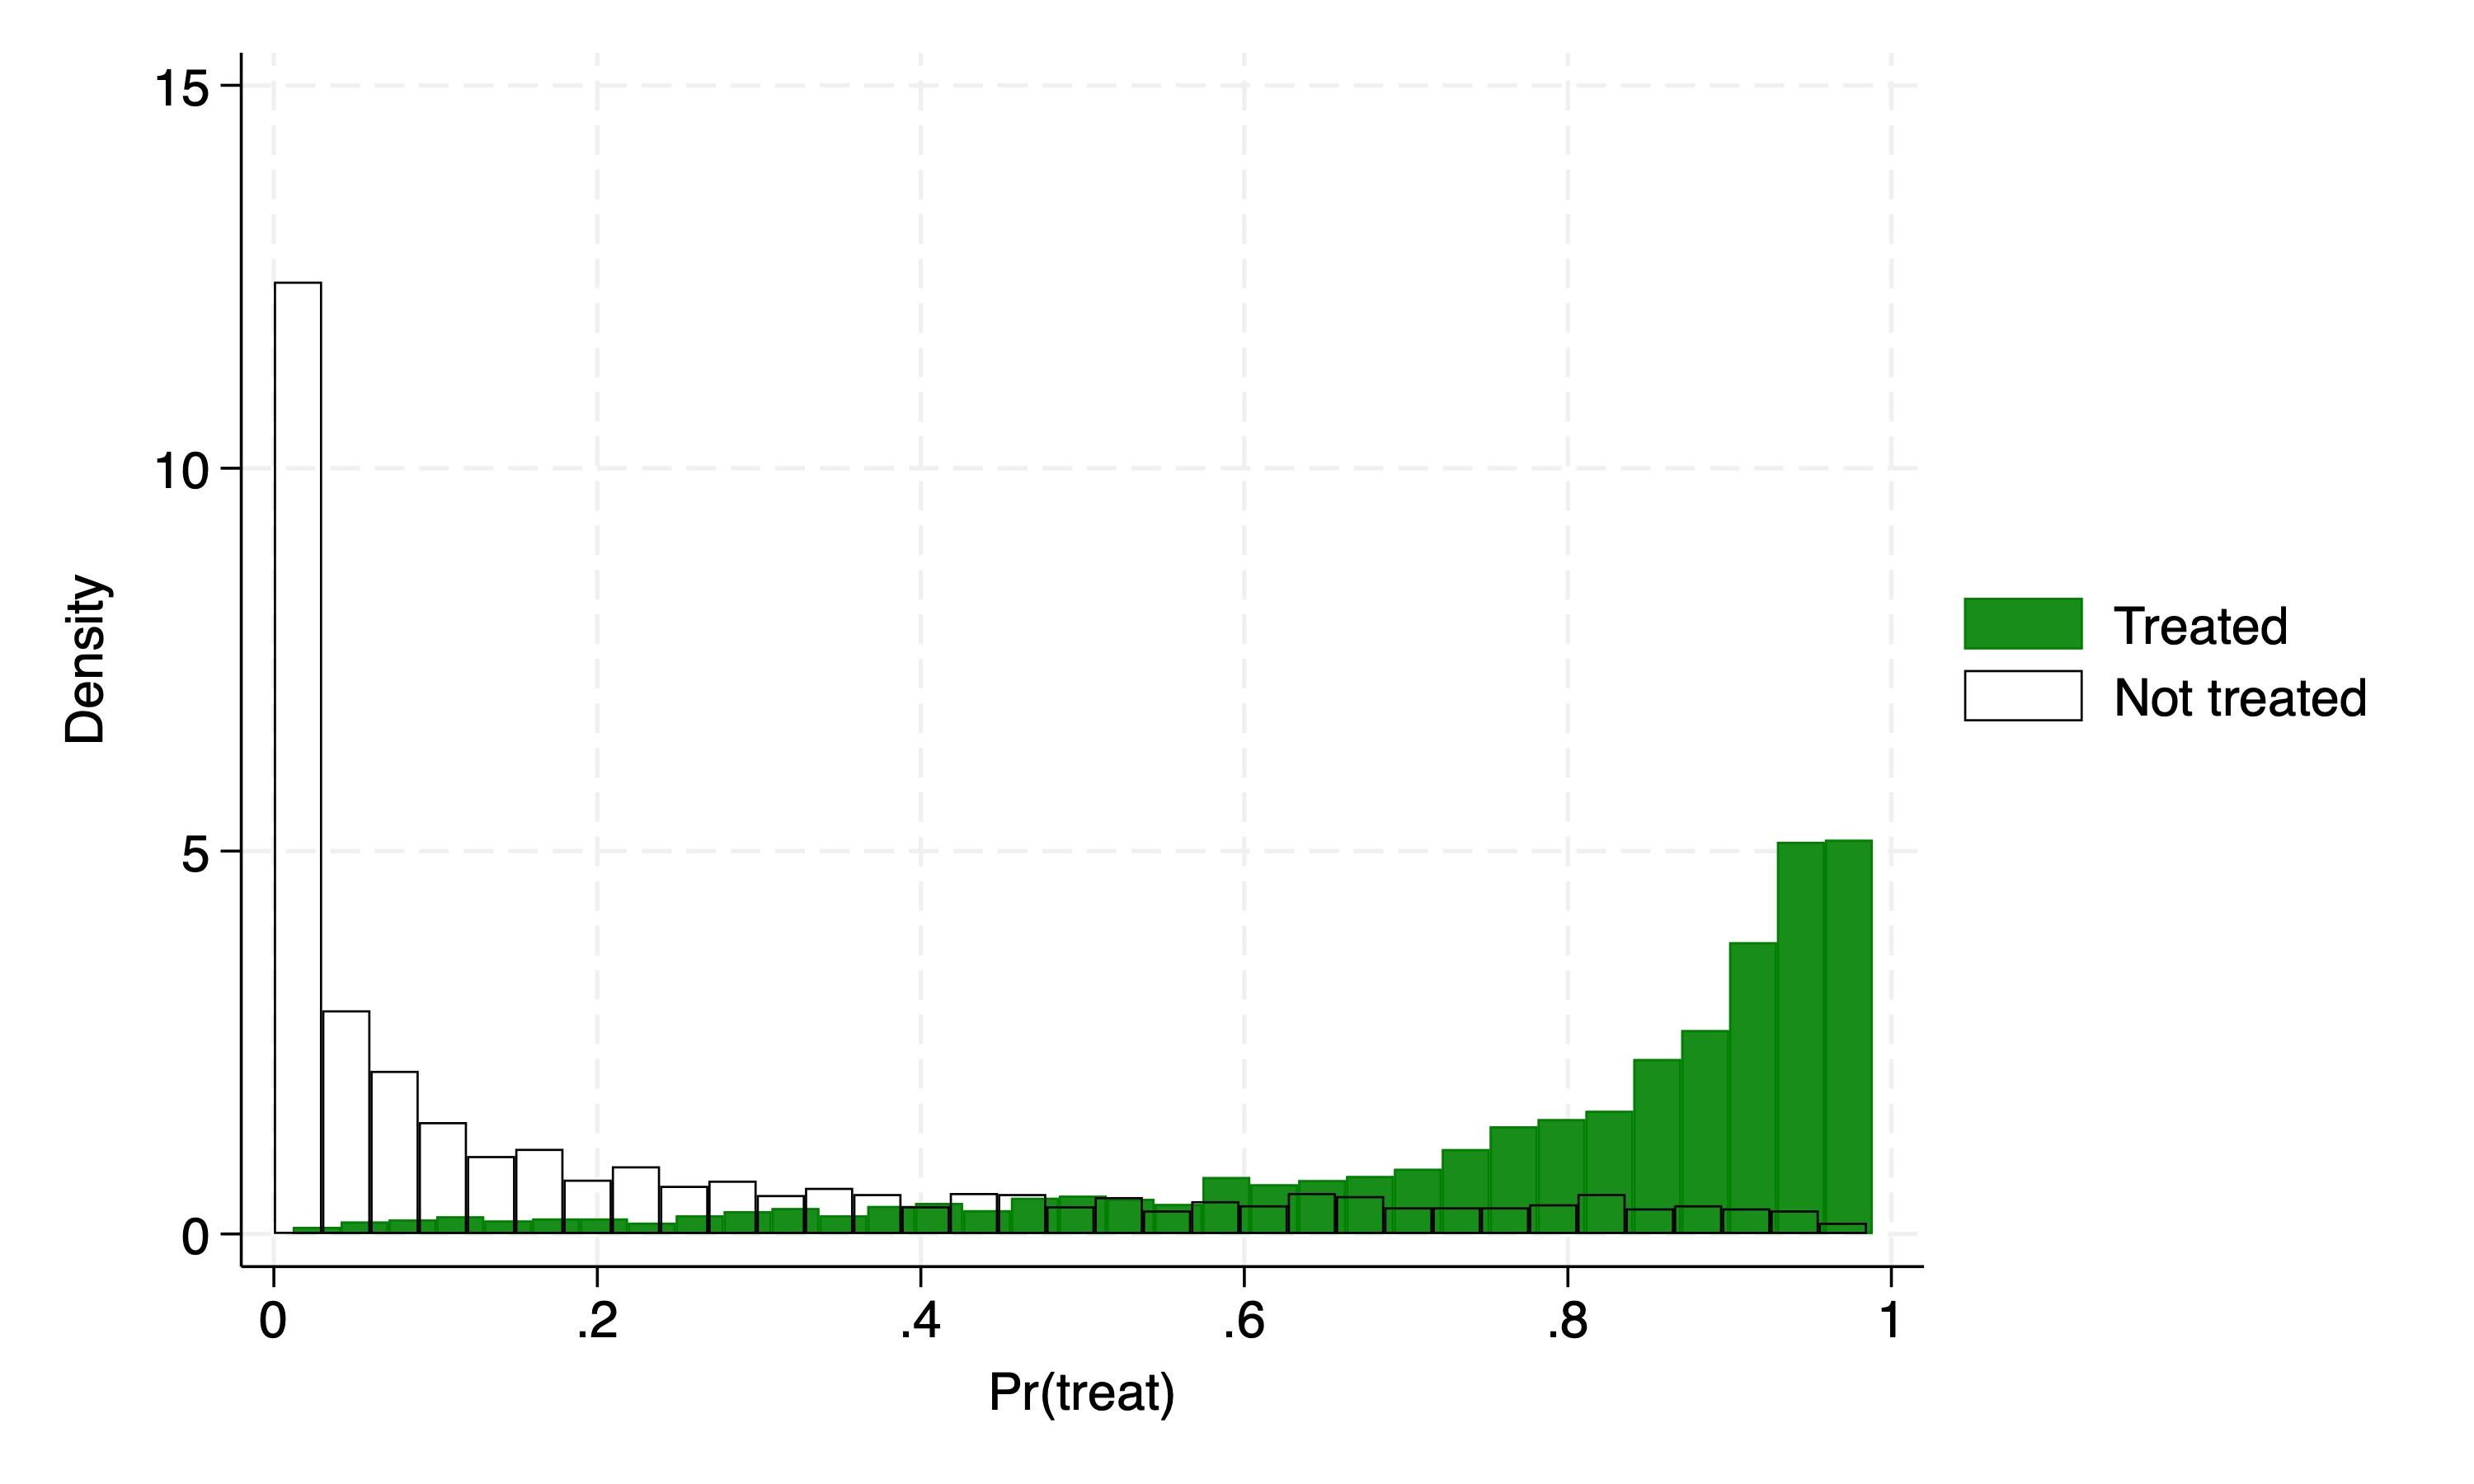
\includegraphics[scale=0.12]{./lecture_includes/pscore_overlap}
\end{figure}

\end{frame}

\begin{frame}{Estimating ATE with IPW}

\begin{itemize}
\item \emph{Any} of the parameters including the ATE are possible with propensity scores

\item Assumptions are strongest for ATE:  full unconfoundedness and full support versus weak versions of both 

\item You should only focus on the ATE if you care about the entire population's treatment effects, but remember that requires more assumptions than if you just focused on the ATT

\end{itemize}

\end{frame}

	


\begin{frame}{Estimating ATE with IPW}

	
		\begin{block}{Estimating ATE with IPW}
	Given $Y^1,Y^0 \independent{D}|X$ and common support, then
		\begin{eqnarray*}
		\delta_{ATE}&=&E[Y^1-Y^0] \\
		&=&E \left[ Y \cdot  \frac{D - \rho(X)}{\rho(X) \cdot (1-\rho(X))} \right]
		\end{eqnarray*}
	\end{block}

Notice that since treated units are missing counterfactuals, but so are controls, all of the data is weighted for the ATE (not just the controls for ATT)

\end{frame}


\begin{frame}{Inverse Probability Weighting}

	\begin{proof}
	\begin{eqnarray*}
	E \left[ Y \cdot \frac{D-\rho(X)}{\rho(X)(1-\rho(X))} \Big\vert X \right] &=& E \left[ \frac{Y}{\rho(X)} \Big\vert X,D=1 \right] \rho(X) \\
	&& + E\left[ \frac{-Y}{1-\rho(X)} \Big\vert X,D=0 \right](1-\rho(X)) \\
	&=& E[Y|X,D=1] - E[Y|X,D=0]
	\end{eqnarray*}and the results follow from integrating over $P(X)$ and $P(X|D=1)$.
	\end{proof}

\end{frame}

\begin{frame}{Other comments about propensity scores}

\begin{itemize}

\item Only other comments to make is that you can get outlier weights
\item If the propensity score is very high for a control group in the ATT, the weight can explode
\item Certain normalizations of the way the IPW is constructed to try and minimize those influences
\item Stata's \texttt{teffects} or R's \texttt{ipw} both let you estimate parameters using IPW and get standard errors
\item But you can do it manually using OLS and use  the propensity scores as analytical weights

\end{itemize}

\end{frame}

\begin{frame}{Simulation}

Lets look at the \texttt{matching.do} again

\end{frame}


\begin{frame}{Double robust estimators}

\begin{itemize}
\item You can have the right covariates but the wrong model and unbiasedness requires the correct model
\item What if you had a way to control for the covariates using propensity scores and something else like regression?
\item Buys you some insurance against model misspecification if such a thing existed
\end{itemize}

\end{frame}

\begin{frame}{Double robust estimators}

\begin{itemize}
\item Question: Is it possible to combine the virtues of regression and propensity score?
\item Answer: Double robust estimators
\item DR address the model misspecification problem by combining propensity scores with other methods 
\item Basic idea in all of them was to control for covariates twice \emph{at the same time} without paying for it (two for one)
\end{itemize}

\end{frame}

\begin{frame}{Double robust estimators}

\begin{itemize}
\item We say that estimators combining regression with IPW are double robust so long as
	\item The regression for the outcome is properly specified, or
	\item The propensity score is properly specified
\item We give ourselves two chances to get it right (either/or not both/and) but if neither is properly specified, then you didn't really gain much
\item Three strikes in baseball
\end{itemize}

\end{frame}

\begin{frame}{Doubly Robust Estimator}
    Easy to verify: with true \( m_1(X) \) (an outcome regression or OR model) and \( \rho(X) \)
\footnotesize

    \[
    ATE = \mathbb{E} \left[ \frac{DY}{\rho(X)} - \frac{D - \rho(X)}{\rho(X)}m_1(X) \right]
    - \mathbb{E} \left[ \frac{(1 - D)Y}{1 - \rho(X)} + \frac{D - \rho(X)}{1 - \rho(X)}m_0(X) \right]
    \]

    \[
    = \mathbb{E} \left[ m_1(X_i) + \frac{D_i\{Y_i - m_1(X_i)\}}{\rho(X_i)} \right]
    - \mathbb{E} \left[ m_0(X_i) + \frac{(1 - D_i)\{Y_i - m_0(X_i)\}}{1 - \rho(X_i)} \right]
    \]

    \[
    = \mu_1 - \mu_0 = \mathbb{E}[Y(1)] - \mathbb{E}[Y(0)]
    \]
\end{frame}

\begin{frame}{Doubly Robust Estimator}
    In the previous formula, replace the true PS \( \rho(X) \) and outcome
    \( m_1(X) \) by the estimated ones from postulated models \( \hat{\rho}(X) \) and
    \( \hat{m}_1(X) \), we obtain two augmented estimators:

    \[
    \widehat{\tau}_{dr} = \hat{\mu}_{1,dr} - \hat{\mu}_{0,dr}
    \]

\footnotesize
    \[
    = \frac{1}{N} \sum_{i=1}^{N} \left[ \frac{D_iY_i - D_i - \hat{\rho}(X_i)}{\hat{\rho}(X_i)} \hat{m}_1(X_i) \right]
    - \frac{1}{N} \sum_{i=1}^{N} \left[ \frac{(1 - D_i)Y_i - D_i - \hat{\rho}(X_i)}{1 - \hat{\rho}(X_i)} \hat{m}_0(X_i) \right]
    \]

\end{frame}

\begin{frame}{Double Robust Estimator}

\begin{itemize}

\item     The two estimators are mathematically the same, but they have different statistical implications:
    	\begin{itemize}
	\item  the first estimator augments an IPW estimator by outcome regression (OR); 
	\item the second augments an OR estimator by IPW.
	\end{itemize}
\item The first estimator is usually referred to as the ``doubly-robust (DR) estimator'' and we saw it in Sant'Anna and Zhou (2020) actually for diff-in-diff

\end{itemize}
\end{frame}


\begin{frame}{Doubly Robust Estimator}
    Now focus on the DR estimator

    Notice that \( \hat{\mu}_{1,dr} \) and \( \hat{\mu}_{0,dr} \) have the same structure

    \[
    \hat{\mu}_{1,dr} = N^{-1} \sum_{i=1}^{N} \left[ \frac{D_iY_i}{\hat{\rho}_i} - \frac{(D_i - \hat{\rho\rho}_i)\hat{m}_1}{\hat{\rho}_i} \right]
    \]

    \[
    \hat{\mu}_{0,dr} = N^{-1} \sum_{i=1}^{N} \left[ \frac{(1 - D_i)Y_i}{1 - \hat{\rho}_i} + \frac{(D_i - \hat{\rho}_i)\hat{m}_0}{1 - \hat{\rho}_i} \right]
    \]

    We will study the properties of \( \hat{\mu}_{1,dr} \) as an estimator for \( \mu_1 = \mathbb{E}\{Y(1)\} \); \( \hat{\mu}_{0,dr} \) is symmetric
\end{frame}




\begin{frame}{Doubly Robust Estimator}
    What does \( \hat{\mu}_{1,dr} \) estimate? Simple algebra shows that \( \mu_{1, dr} \) converges to

    \[
    \mathbb{E}\left[ \frac{DY}{\rho(X)} - \frac{D - \rho(X)}{\rho(X)}m(X) \right]
    \]

    \[
    = \mathbb{E}\{Y(1)\} + \mathbb{E}\left[ \frac{D - \rho(X)}{\rho(X)}\{Y(1) - m(X)\} \right]
    \]


\begin{itemize}
\item     Thus, in order for \( \hat{\mu}_{1,dr} \) to estimate \( \mathbb{E}\{Y(1)\} \), the second term in (4) must be 0

\item     Regression estimator augmented by weighted residuals

\item     When does the second term $=$ 0?

\end{itemize}
\end{frame}

\begin{frame}{Doubly Robust Estimator}
    When does \( R = \mathbb{E} \left[ \frac{D - \rho(X)}{\rho(X)} \{Y(1) - m_1(X)\} \right] = 0? \)

    \begin{itemize}
        \item \textbf{Scenario 1:} Postulated propensity score model \( \rho(X; \beta) \) is
        incorrect, but postulated regression model \( m_1(X; \alpha) \) is correct

        \[
        R = \mathbb{E} \left[ \mathbb{E} \left[ \frac{D - \rho(X)}{\rho(X)} \{Y(1) - m_1(X)\} \middle| X \right] \right]
        \]

        \[
        = \mathbb{E} \left[ \frac{\rho_{true}(X) - \rho(X)}{\rho(X)} \mathbb{E} \{Y(1) - m_1(X) \middle| X\} \right]
        \]

\item Easy to see that \( \mathbb{E} \{Y(1) - m_1(X) | X\} = \mathbb{E} \{Y(1) | X\} - m_1(X) = m_{1,true}(X) - m_1(X) = 0 \)

    \end{itemize}
\end{frame}


\begin{frame}{Doubly Robust Estimator}
    When does \( \mathbb{E} \left[ \frac{D - \rho(X)}{\rho(X)} \{Y(1) - m_1(X)\} \right] = 0? \)

    \begin{itemize}
        \item \textbf{Scenario 2:} Postulated propensity score model \( \rho(X; \beta) \) is correct,
        but postulated regression model \( m_1(X; \alpha) \) is incorrect

        \[
        R = \mathbb{E} \left[ \mathbb{E} \left[ \frac{D - \rho(X)}{\rho(X)} \{Y(1) - m_1(X)\} \middle| X \right] \right]
        \]

        \[
        = \mathbb{E} \left[ \frac{\hat{e}_{true}(X) - \rho(X)}{\rho(X)} \mathbb{E} \{Y(1) - m_1(X) \middle| X\} \right]
        \]

        \item Equals to zero because \( \hat{\rho}_{true}(X) - \rho(X) = 0 \)
    \end{itemize}
\end{frame}




\begin{frame}{Doubly Robust Estimator}
    \begin{itemize}
        \item In both cases, the second term goes to 0 in large samples, and
        thus \( \hat{\mu}_{1,dr} \) is consistent (asymptotically unbiased) for \( E(Y(1)) \).
        \item Similarly, \( \hat{\mu}_{0,dr} \) is consistent for \( E(Y(0)) \), and hence \( \hat{\tau}_{dr} \)
        is consistent for the ATE.
        \item Obviously, if both models are correct, \( \hat{\tau}_{dr} \) is consistent for
        estimating the ATE.
    \end{itemize}
\end{frame}




\begin{frame}{Doubly Robust Estimator}
    \textbf{Double Robustness:} \( \hat{\tau}_{dr} \) is a consistent estimator of the ATE if either
    the propensity score model or the potential outcome model is, but not
    necessarily both are, correctly specified

    \begin{itemize}
        \item DR is a large sample property
        \item Offers protection against model mis-specification: gives you two
        chances to get it right (and wrong)!
        \item If \( \rho(X) \) and \( m_1(X) \) are modeled correctly, \( \hat{\tau}_{dr} \) will have smaller
        variance than the IPW estimator (in large samples)
        \item If the outcome model \( m_1(X) \) is correct, \( \hat{\tau}_{dr} \) has larger variance (in
        large samples) than the direct regression estimator
        \item ... but gives protection in the event it is not
    \end{itemize}
\end{frame}








\begin{frame}{Propensity score matching}
	
	\begin{itemize}
	\item Matching, or ``imputation'', is another way that utilizes the $\widehat{\rho_i}(X_i)$
	\item Matching estimation based on the propensity score has the same first step as IPW, but not the second and third steps
	\item Common support starts to be more complex with imputation methods because you will need to decide how far away from a unit's own propensity score is a tolerable distance to be considered a ``neighbor''
	\end{itemize}

\end{frame}




\begin{frame}{Standard matching strategy}
	
	\begin{itemize}
	\item Pair each treatment unit $i$ with one or more \emph{comparable} control group unit $j$, where comparability is in terms of proximity, or distance, to the estimated propensity score
	\item Impute the unit's missing counterfactual outcome $Y_{i(j)}$ based on the unit or units chosen in the previous step
	\item If more than one are ``nearest neighbors'', then use the neighbors' weighted outcomes  $$Y_{i(j)} = \sum_{j \in C(i)} w_{ij}Y_j$$ where $C(i)$ is the set of neighbors with $W=0$ of the treatment unit $i$and $w_{ij}$ is the weight of control group units $j$ with $\sum_{j \in C(i)} w_{ij} = 1$
	\end{itemize}
\end{frame}


\begin{frame}{Imputing the counterfactuals}
	
	Let the ATT be our parameter of interest: $$E[Y^1_i | D_i=1] - E[Y^0_i | D_i=1]$$We estimate it as follows  $$\widehat{ATT} = \frac{1}{N_T}  \sum_{i:D_i=1} \bigg [Y_i - Y_{i(j)} \bigg ]$$where $N_T$ is the number of matched treatment units in the sample. Note the difference between \emph{imputation} and IPW -- the only weight here is $\frac{1}{N_T}$

\end{frame}

\begin{frame}{Matching methods}
	
	\begin{itemize}
	\item The probability of observing two units with \emph{exactly} the same propensity score is in principle zero if $Pr(X=x)$ is continuous
	\item Several matching methods have been proposed in the literature, but the most widely used are:
		\begin{itemize}
		\item Stratification matching
		\item Nearest-neighbor matching (with or without caliper)
		\item Radius matching
		\item Kernel matching
		\end{itemize}
	\item Typically, one treatment unit $i$ is matched to several control units $j$, but sometimes one-to-one matching is used
	\end{itemize}
	
\end{frame}


\begin{frame}{Stratification}
	
	\begin{itemize}
	\item Stratification based on the propensity score is a multi step process that bears resemblance to the stratification/subclassification method proposed by Cochran (1968)
	\item  Method uses brute force to achieve the balancing property discussed earlier, which is then used with weighted differences in means within propensity score ``strata''
	\item Dehejia and Wahba (2002) used stratification matching in their seminal paper 
	\end{itemize}
	
\end{frame}


\begin{frame}{Stratification: Achieving Balance}
	
First create ``propensity score strata'' inside which you have balanced covariates
	\begin{enumerate}
		\item Sort the data by propensity score and divide into groups of observations with similar propensity scores (e.g., percentiles)
		\item Within each strata, test (e.g., t-test) whether the means of the $k$ covariates are equal between treatment and control
		\item If so, then stop.  If not, it means the covariates aren't balanced \emph{within that propensity score strata} so then divide that strata in half and repeat step 2
		\item If a particular covariate is unbalanced for multiple groups, modify the initial logit or probit equation by including higher order terms and/or interactions with that covariate and repeat
		\end{enumerate}

\end{frame}

\begin{frame}{Propensity score matching}
	
	\begin{itemize}
	\item Next we review explicit imputation based on the propensity score or what is sometimes called propensity score matching
	\item King and Nielsen (2019) is a critique of using propensity scores \emph{for matching} (i.e., imputation)
	\item But not a critique of the propensity score itself or to stratification, regression adjustment, or IPW
	\item Issues raised have to do with forced balance through trimming and a myriad of other common choices made by the researcher
	\end{itemize}
	
\end{frame}

\begin{frame}{Ad hoc user choices introduce bias}

\begin{quote}
	
```[The] more balanced the data, or the more balance it becomes by [trimming] some of the observations through matching, the more likely propensity score matching will degrade inferences.'' -- King and Nielsen (2019)

\end{quote}
	
\end{frame}



\begin{frame}{Nearest Neighbor}
	
	Pretty similar to covariate matching.  Formula is $$\widehat{ATT} = \frac{1}{N_T} \sum_{i:D_i=1} \bigg [ Y_i - \sum_{j \in C(i)_M} w_{ij}Y_j \bigg ]$$ 
		\begin{itemize}
		\item $N_T$ is the number of treated units $i$ and  $N_C$ is number of control units $j$
		\item $w_{ij}$ is equal to $\frac{1}{N_C}$ if $j$ is a control unit and zero otherwise
		\item And unit $j$ is chosen as a control for $i$ if it's propensity score is nearest to that of $i$
		\end{itemize}
\end{frame}

\begin{frame}{NN Matching: Bias vs. Variance}
	
How far away on the propensity score will you use is what makes some of the different types of matching proposed differ
		\begin{itemize}
		\item Matching just one nearest neighbor minimizes bias at the cost of larger variance
		\item Matching using additional nearest neighbors increases the bias but decreases the variance
		\end{itemize}
	
\end{frame}

\begin{frame}{NN Matching: Bias vs. Variance}
	
	 Matching with or without replacement
		\begin{itemize}
		\item with replacement keeps bias low at the cost of larger variance
		\item without replacement keeps variance low but at the cost of potential bias
		\end{itemize}
	
\end{frame}



\begin{frame}{Distance between treatment and control units}

\begin{itemize}
\item What was historically done was limiting ``distance''  through various \emph{ad hoc} choices
\item Imagine these choices as creating like a cowboy rope lasso that matches to everything inside that circle
\item There were two common ways for creating the circle -- caliper matching and radius matching. 
\end{itemize}

\end{frame}

\begin{frame}{Caliper matching}
	
	\begin{itemize}
	\item Caliper matching is a variation on NN matching that tries to build brakes into the algorithm as to avoid ``bad neighbors'' by imposing a tolerable maximum distance (e.g., 0.2 units in the propensity score away from a treatment unit $i$'s propensity score)
	\item Note -- this is a one-to-one imputation, and if there doesn't exist anybody in the control group unit $j$ within that ``caliper'', then treatment unit $i$ is discarded which as with all trimming changes the parameter we are estimating
	\item It's difficult to know what this caliper should be \emph{ex ante}, hence why I said it is somewhat \emph{ad hoc}
	\end{itemize}

\end{frame}


\begin{frame}{Radius matching}
	
	
		\begin{itemize}
		\item Each treatment unit $i$ is matched with the control group units whose propensity score are in a ``predefined neighborhood'' of the propensity score of the treatment unit.
		\item \textbf{All} the control units with $\widehat{\rho_j}(X_{j})$ falling within a radius $r$ from $\widehat{\rho}_i(X_i)$ are matched to the treatment unit $i$ -- this is what distinguishes it from calipers, and makes it more similar to covariate matching (Abadie and Imbens 2006, 2008)
		\item The smaller the radius, the better the quality of the matches, but the higher the possibility some treatment units are not matched because the neighborhood does not contain control group units $j$
		\end{itemize}
		
\end{frame}

\begin{frame}{Software}

\begin{itemize}
\item You can use -\texttt{teffects, psmatch}- to get at these two nearest neighbor approaches by setting the number of matches
\item You can use -\texttt{pscore2}- for stratification
\item You can use the \texttt{MatchIt} package in R
\end{itemize}

\end{frame}





		  

\begin{frame}{Failure of econometric estimators (LaLonde 1986)}
	
	\begin{itemize}
	\item Evaluation of the Job Trainings Program (NSW) has a rich history in causal inference
	\item Bob LaLonde (passed away November 2015) was a Card and Ashenfelter student at Princeton whose job market paper evaluated, not NSW itself, but econometric methods one would use in something like NSW
	\item Dehejia and Wahba (1999; 2002) used LaLonde's data with propensity score matching and found they could recover known effects
	\item Critiques by Petra Todd, Jeff Smith and others followed which I'll summarize
	\end{itemize}
\end{frame}

\begin{frame}{Summarizing LaLonde (1986)}

		\begin{itemize}
		\item Very clever study that combined experimental and non-experimental data to ascertain whether popular econometric methods could recover unbiased effects when those effects were already known 
		\item Damning conclusion -- 1986 AER (it was LaLonde's JMP) found econometric methods failed to get the number right, and worse, failed to get the sign right
		\item Was a critical paper in the emerging ``credibility crisis'' within labor and helped fuel the type of work we now broadly consider to be design based causal inference
		\end{itemize}

\end{frame}

\begin{frame}[plain]
	\begin{center}
	LaLonde, Robert J. (1986). \myurlshort{http://business.baylor.edu/scott_cunningham/teaching/lalonde-1986.pdf}{``Evaluating the Econometric Evaluations of Training Programs with Experimental Data''}. \emph{American Economic Review}. 
	\end{center}
	
\underline{LaLonde's study} was \textbf{not} an evaluation of the NSW program, as that had been done, but rather an evaluation of econometric models done by:
		\begin{itemize}
		\item replacing the experimental NSW control group with non-experimental control group drawn from two nationally representative survey datasets: Current Population Survey (CPS) and Panel Study of Income Dynamics (PSID)
		\item estimating the average effect using non-experimental workers as controls for the NSW trainees 
		\item comparing his non-experimental estimates to the experimental estimates of \$900
		\end{itemize}
\end{frame}

\begin{frame}{LaLonde (1986)}

\begin{itemize}

	\item \underline{LaLonde's conclusion}: available econometric approaches were biased and inconsistent
		\begin{itemize}
		\item His estimates were way off and usually the wrong sign
		\item Conclusion was influential in policy circles and led to greater push for more experimental evaluations
		\end{itemize}

\end{itemize}

\end{frame}


\begin{frame}{Description of NSW Job Trainings Program}
	
The National Supported Work Demonstration (NSW), operated by Manpower Demonstration Research Corp in the mid-1970s:
	\begin{itemize}
	\item was a temporary employment program designed to help disadvantaged workers lacking basic job skills move into the labor market by giving them work experience and counseling in a sheltered environment
	\item was also unique in that it \textbf{randomly assigned} qualified applicants to training positions:
		\begin{itemize}
		\item \textbf{Treatment group}: received all the benefits of NSW program
		\item \textbf{Control group}: left to fend for themselves
		\end{itemize}
	\item admitted AFDC females, ex-drug addicts, ex-criminal offenders, and high school dropouts of both sexes
	\end{itemize}
\end{frame}

\begin{frame}{NSW Program}
	
	\begin{itemize}
	\item Treatment group members were:
		\begin{itemize}
		\item guaranteed a job for 9-18 months depending on the target group and site
		\item divided into crews of 3-5 participants who worked together and met frequently with an NSW counselor to discuss grievances and performance
		\item paid for their work
		\end{itemize}
	\item Control group members were randomized so the same
	\item Note: the randomization balanced observables and unobservables across the two arms, thus enabling the estimation of an ATE for the people who self-selected into the program
	\end{itemize}
\end{frame}

\begin{frame}{NSW Program}

\begin{itemize}
	\item Other details about the NSW program:
		\begin{itemize}
		\item \underline{Wages}:  NSW offered the trainees lower wage rates than they would've received on a regular job, but allowed their earnings to increase for satisfactory performance and attendance
		\item \underline{Post-treatment}: after their term expired, they were forced to find regular employment
		\item \underline{Job types}:  varied within sites -- gas station attendant, working at a printer shop -- and males and females were frequently performing different kinds of work
		\end{itemize}
\end{itemize}

\end{frame}
	
\begin{frame}{NSW Data}
	
	\begin{itemize}
	\item \underline{NSW data collection}:
		\begin{itemize}
		\item MDRC collected earnings and demographic information from both treatment and control at baseline and every 9 months thereafter
		\item Conducted up to 4 post-baseline interviews
		\item Different sample sizes from study to study can be confusing, but has simple explanations
		\end{itemize}
	\end{itemize}
\end{frame}
	

\begin{frame}{NSW Data}

\begin{itemize}
	\item \underline{Estimation}:
		\begin{itemize}
		\item NSW was a randomized job trainings program; therefore estimating the average treatment effect is straightforward:
			\begin{eqnarray*}
			SDO = \frac{1}{N_t}\sum_{D_i=1}Y_i - \frac{1}{N_c}\sum_{D_i=0}Y_i \approx E[Y^1-Y^0] 
			\end{eqnarray*}in large samples assuming treatment selection is independent of potential outcomes (randomization) -- i.e., $(Y^0,Y^1)\independent{D}$. 
		\end{itemize}
	\item \underline{NSW worked}: Treatment group participants' real earnings post-treatment (1978) was positive and economically meaningful -- $\approx$ \$900 (LaLonde 1986) to \$1,800 (Dehejia and Wahba 2002) depending on the sample used
\end{itemize}

\end{frame}
	
\imageframe{./lecture_includes/lalonde_table5a.png}


\begin{frame}{Switching out the control group}

\begin{itemize}
\item Think of \$800 to \$900 as the ``ground truth'' since row 1 was using the RCT 
\item LaLonde ``drops'' the experimental controls (which satisfied independence) and ``replaces'' it with six different draws from two nationally representative surveys (PSID and CPS)
\item Now the dataset contains a negatively selected treatment group compared to a nationally representative control group
\item Will selection on observable methods ``work''?
\end{itemize}

\end{frame}


\imageframe{./lecture_includes/lalonde_table5b.png}

\begin{frame}[plain,shrink=10]{Imbalanced covariates for experimental and non-experimental samples}

    \begin{center}
		\begin{table}
		\begin{tabular}{lcccccc}
		\hline \hline
		\multicolumn{3}{c}{}&
		\multicolumn{1}{c}{CPS}&
		\multicolumn{1}{c}{NSW}\\
		
		\multicolumn{1}{c}{}&
		\multicolumn{2}{c}{All} &
		\multicolumn{1}{c}{Controls} &
		\multicolumn{1}{c}{Trainees} \\

		\multicolumn{3}{c}{}&
		\multicolumn{1}{c}{$N_c=15,992$}&
		\multicolumn{1}{c}{$N_t=297$}&
		\multicolumn{1}{c}{}&
		\multicolumn{1}{c}{}\\

		\multicolumn{1}{l}{covariate}&
		\multicolumn{1}{c}{mean}&
		\multicolumn{1}{c}{(s.d.)}&
		\multicolumn{1}{c}{mean}&
		\multicolumn{1}{c}{mean}&
		\multicolumn{1}{c}{t-stat}&
		\multicolumn{1}{c}{diff}\\
		\hline
Black    & 0.09 & 0.28 & 0.07 & 0.80 & 47.04 & -0.73\\
Hispanic & 0.07 & 0.26 & 0.07 & 0.94 & 1.47 & -0.02\\
Age & 33.07 & 11.04 & 33.2 & 24.63 & 13.37  & 8.6\\
Married & 0.70 & 0.46 & 0.71 & 0.17 & 20.54 & 0.54\\
No degree & 0.30 & 0.46 & 0.30 & 0.73 & 16.27 & -0.43\\
Education & 12.0 & 2.86 & 12.03 & 10.38 & 9.85 & 1.65 \\
1975 Earnings   & 13.51 & 9.31 & 13.65 & 3.1 & 19.63 & 10.6\\
1975 Unemp  & 0.11 & 0.32 & 0.11 & 0.37 & 14.29 & -0.26\\
		\hline 
		\end{tabular}
		\end{table}
    \end{center}

\end{frame}


\begin{frame}{Dehija and Wahba (1999)}
	
	\begin{itemize}
	\item Dehejia and Wahba (DW) update LaLonde's original study using propensity score matching
		\begin{enumerate}
		\item Dehejia, Rajeev H. and Sadek Wahba (1999). 	``Causal Effects in Nonexperimental Studies: Reevaluating the Evaluation of Training Programs''. \underline{Journal of the American Statistical} \underline{Association}, vol. 94(448): 1053-1062 (\myurlshort{http://business.baylor.edu/scott_cunningham/teaching/dehejia-and-wahba-1999.pdf}{pdf})
		\end{enumerate}
	\item Can propensity score matching improve over the estimators that LaLonde examined?
	\end{itemize}
\end{frame}

\begin{frame}[plain]
	
\begin{figure}
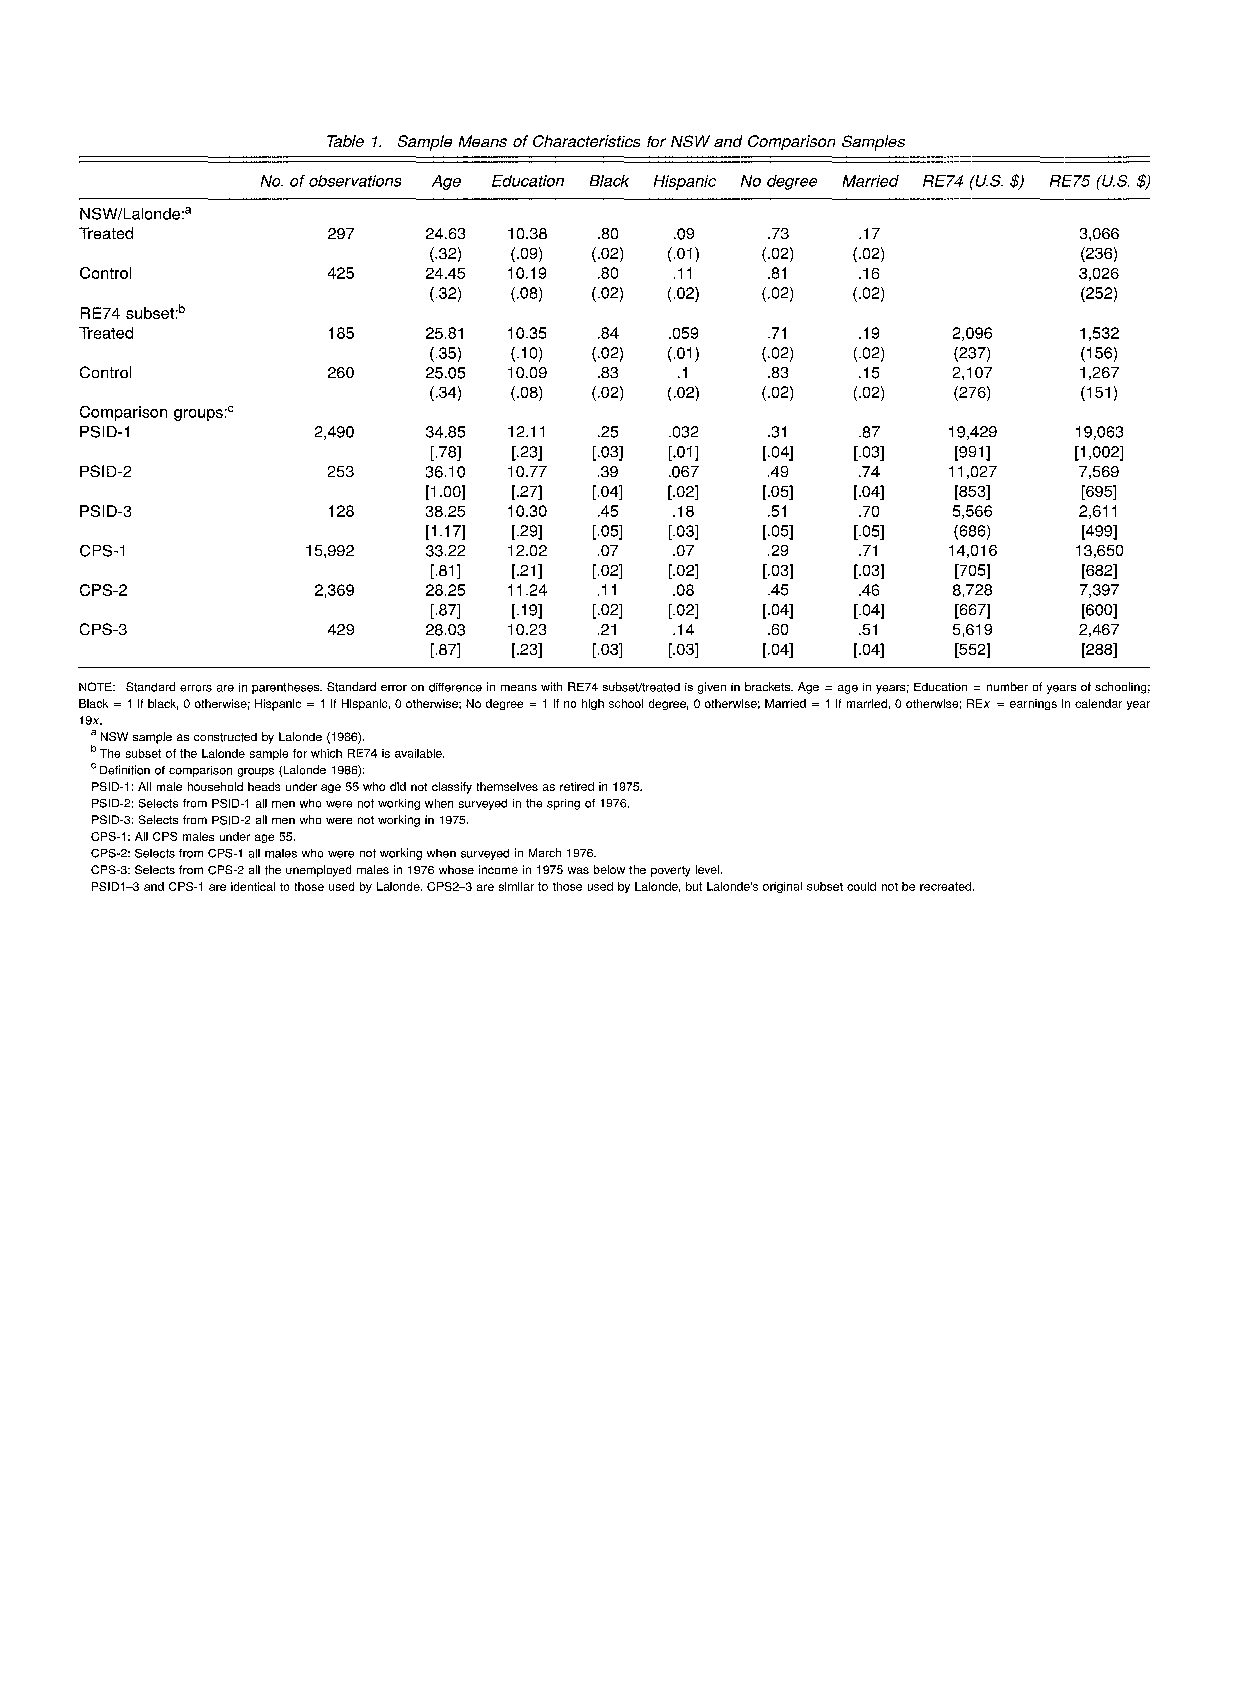
\includegraphics[scale=0.5]{./lecture_includes/dw_1.pdf}
\end{figure}

\end{frame}

\imageframe{./lecture_includes/dw_2.pdf}

\begin{frame}{Covariate imbalance}
	

	\begin{itemize}
	\item Conditional on the propensity score, the covariates are independent of the treatment, suggesting that the distribution of covariate values should be the same for both treatment and control groups
	\item This can be checked as we have data on all three once we've estimated the propensity score
	\item DW note that the two samples have \emph{severe} imbalance on \emph{observables} -- a huge number of non-experimental controls have propensity scores almost exactly equal to 0
	\item Their analysis will ``trim'' (which will ultimately have implications for interpretation)
	\end{itemize}

\end{frame}



\imageframe{./lecture_includes/dw_3.pdf}
\imageframe{./lecture_includes/dw_4.pdf}
\imageframe{./lecture_includes/dw_5.pdf}
\imageframe{./lecture_includes/dw_6.pdf}



\clearpage
\newpage

\begin{frame}{Replies by econometricians to DW}

\begin{itemize}
\item Heckman, Smith and Todd concluded from their own work that in order for matching estimators to have low bias, you need the following:
	\begin{enumerate}
	\item A rich set of variables related to program participation and predictive of $Y^0$ labor market outcomes, 
	\item Nonexperimental comparison group be drawn from the same local labor markets as the participants and 
	\item Dependent variable (e.g., earnings) be measured in the same way for participants and nonparticipants
	\end{enumerate}
\item All three of these conditions fail to hold in DW (1999, 2002) according to Smith and Todd (2005)
\item DW also note the importance of conditioning on pre-treatment lagged outcomes (e.g., real earnings in $t-1$, $t-2$, etc.) as well as \emph{trimming}
\end{itemize}

\end{frame}


\begin{frame}{Smith and Todd, diff-in-diff, doubly robust}

\begin{itemize}
\item Difference-in-differences with propensity scores tended to work well in Smith and Todd (2005) though the effect sizes are much larger
\item In my Causal Inference II workshop, we use Sant'anna And Zhao's double robust DiD and get nearly the exact same parameter estimate as the experimental finding

\end{itemize}

\end{frame}

\begin{frame}{Coding together}

\begin{itemize}

\item Let's spend some time together trying to replicate the Lalonde study ourselves
\item I use replicate lightly -- our goal is syntax only
\item It's in the Lalonde lab on githbub for this workshop

\end{itemize}

\end{frame}


\subsection{Regressions}



\begin{frame}{Interpreting OLS coefficients}

\begin{itemize}
\item Most common causal model is OLS with covariate controls 


		\begin{align*}
		Y_i = \beta_0 + \beta_1 X_i + u_i&\\
		\end{align*}

\item OLS is the best linear predictor (Angrist and Pischke 2009)
\item But the best linear predictor of the \emph{realized} outcome is not the same as being the best linear predictor of the \emph{missing potential outcome}

\end{itemize}

\end{frame}



\begin{frame}{OLS Simulated Code}

\begin{figure}[!t]\centering
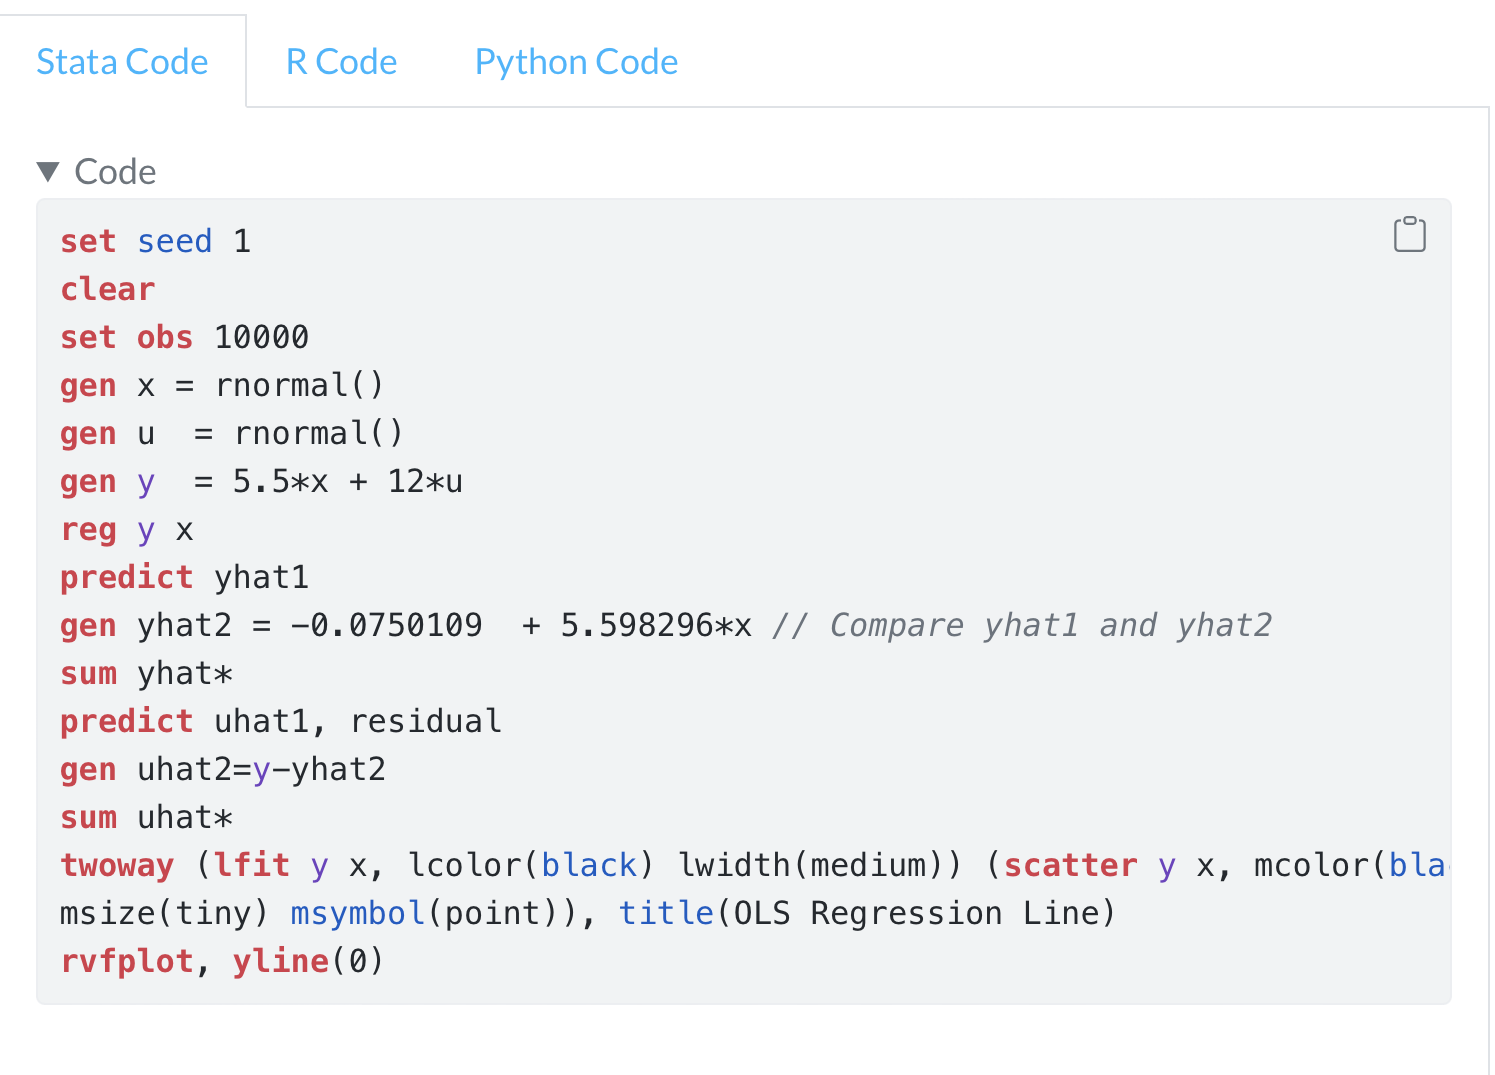
\includegraphics[scale=0.40]{./lecture_includes/ols_code}
\end{figure}

\end{frame}

\begin{frame}{OLS Extrapolates Using Functional Form (e.g., Lines)}

\begin{figure}[!t]\centering
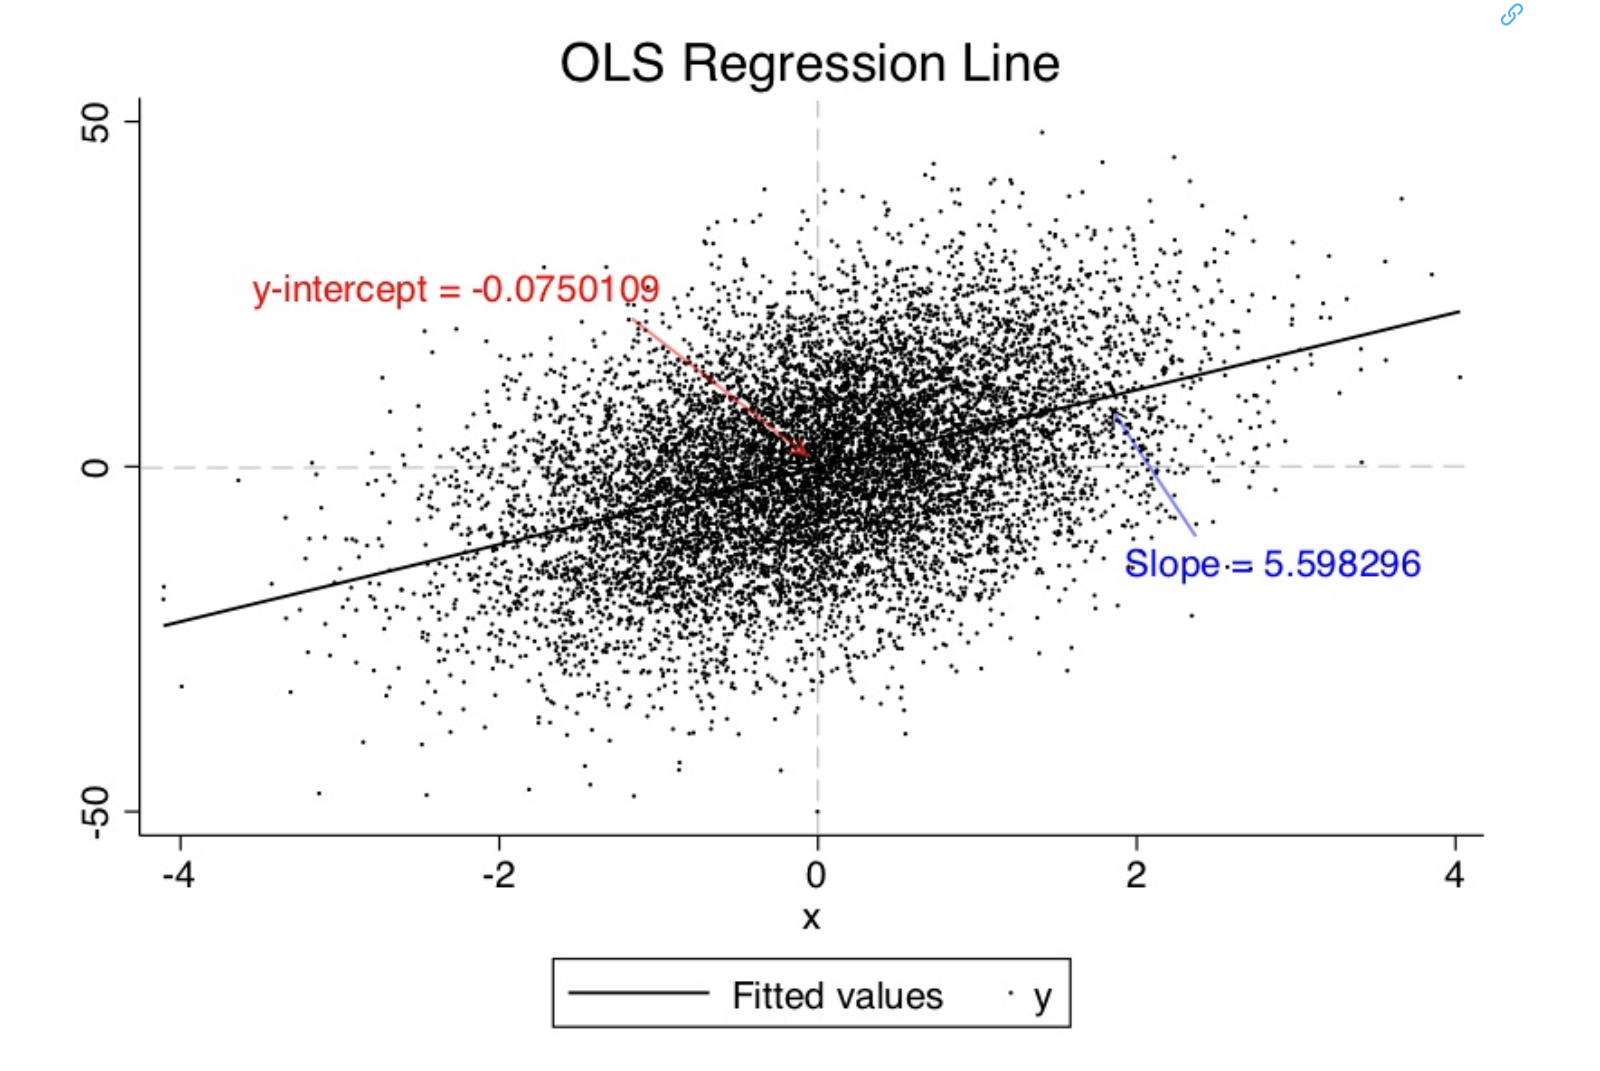
\includegraphics[scale=0.4]{./lecture_includes/ols_line}
\end{figure}

\end{frame}

\begin{frame}{Bivariate vs multivariate regressions}

\begin{itemize}

\item Interpreting the OLS coefficient in bivariate regression is written out as a scaled covariance:

 $$\widehat{\beta_1}=\frac{Cov(Y_i,X_i)}{Var(X_i)}$$
 
 \item But when we are looking at a multivariate regression, what is it?
 
 \end{itemize}
 
 \end{frame}
 
 \begin{frame}{Applying FWL theorem}

\begin{itemize}
\item Frisch-Waugh-Lovell also helps us interpret $\widehat{\beta}_1$ when there are covariates
 \item Use the FWL theorem to turn the multivariate regression coefficient into the simple bivariate one
\item Angrist and Pischke (2009) call FWL the ``regression anatomy theorem'' and Filoso (2013) has an excellent and original proof
\end{itemize}

\end{frame}



\begin{frame}{Applying FWL theorem}

	\begin{itemize}
	\item Can we estimate the causal effect of family size on labor supply by regressing labor supply (\texttt{Y}) on family size (\texttt{X})?
		\begin{eqnarray*}
		Y_i = \beta_0 + \beta_1 X_i + u_i&\\
		\end{eqnarray*}
	\item If family size is random, then we can interpret $\widehat{\beta_1}$ as the ATE
	\item But how do we interpret $\widehat{\beta_1}$ if \texttt{family size} is only conditionally random?  
	\end{itemize}
\end{frame}


\begin{frame}{Applying FWL theorem}
	
	\begin{itemize}
	\item Assume the longer model is:
		\begin{eqnarray*}
Y_i &=& \beta_0 + \beta_1 X_i + \gamma_1 \texttt{White}_i + \gamma_2 \texttt{Married}_i \\
		& & + \gamma_3 \texttt{Age}_i + \gamma_4 \texttt{Employed}_i + u_i
		\end{eqnarray*}
	\item Assume unconfoundedness and constant treatment effects so that family size is independent conditional on all controls
	\item FWL shows that in a multivariate regression, any one coefficient fitted can be reconceived as a simple scaled covariance of the outcome and residualized treatment variable
	\end{itemize}
	
\end{frame}




		

\begin{frame}{FWL Theorem}

	\begin{block}{FWL Theorem }
	Assume your main multiple regression model of interest:$$y_i=\beta_0 + \beta_1x_{1i} + \dots + \beta_kx_{ki} + \dots + \beta_Kx_{Ki} + e_i$$ and an auxiliary regression in which the variable $x_{1i}$ is regressed on all the remaining independent variables$$x_{1i} = \gamma_0 + \gamma_{k-1}x_{k-1 i}+\gamma_{k+1}x_{k+1 i} + \dots + \gamma_Kx_{Ki}+f_i$$and $\tilde{x}_{1i} = x_{1i} - \widehat{x}_{1i}$ being the residual from the auxiliary regression. The parameter $\beta_1$ can be rewritten as:$$\beta_1=\frac{Cov(y_i,\tilde{x}_{1i})}{Var(\tilde{x}_{1i})}$$

	\end{block}

\end{frame}


\begin{frame}[plain, shrink=20]

\bigskip

	\begin{block}{FWL Proof  (Proof by Filoso 2013)}
	To prove the theorem, note $E[\tilde{x}_{ki}]=E[x_{ki}]-E[\widehat{x}_{ki}]=E[f_i]$, and plug $y_i$ and residual $\tilde{x}_{ki}$ from $x_{ki}$ auxiliary regression into the covariance $cov(y_i, \tilde{x}_{ki})$
	\begin{eqnarray*}
	\beta_k &=& \frac{ cov(y_i, \tilde{x}_{ki})}{var(\tilde{x}_{ki})} \\
			 &=& \frac{ cov(\beta_0 + \beta_1x_{1i} + \dots + \beta_kx_{ki} + \dots + \beta_Kx_{Ki} + e_i, \tilde{x}_{ki})}{var(\tilde{x}_{ki})} \\
			&=& \frac{ cov(\beta_0 + \beta_1x_{1i} + \dots + \beta_kx_{ki} + \dots + \beta_Kx_{Ki} + e_i,f_i)}{var(f_i)}
	\end{eqnarray*}
	\begin{enumerate}
	\item Since by construction $E[f_i]=0$, it follows that the term $\beta_0E[f_i]=0$.
	\item Since $f_i$ is a linear combination of all the independent variables with the exception of $x_{ki}$, it must be that$$\beta_1E[f_ix_{1i}] = \dots = \beta_{k-1}E[f_ix_{k-1 i}] = \beta_{k+1}E[f_ix_{k+1 i}] = \dots = \beta_KE[f_ix_{KI}] = 0$$
	\end{enumerate}
	\end{block}
\end{frame}


\begin{frame}[plain, shrink=20]

	\begin{block}{FWL Proof  (Proof by Filoso 2013)}
		\begin{enumerate}\addtocounter{enumi}{2}
		\item Consider now the term $E[e_if_i]$.  This can be written as:
			\begin{eqnarray*}
			E[e_if_i] &=& E[e_if_i] \\
			&=& E[e_i\tilde{x}_{ki}] \\
			&=& E[e_i(x_{ki} - \widehat{x}_{ki})] \\
			&=& E[e_ix_{ki}] - E[e_i\tilde{x}_{ki}]
			\end{eqnarray*}Since $e_i$ is uncorrelated with any independent variable, it is also uncorrelated with $x_{ki}$: accordingly, we have $E[e_ix_{ki}]=0$. With regard to the second term of the subtraction, substituting the predicted value from the $x_{ki}$ auxiliary regression, we get$$E[e_i\tilde{x}_{ki}] = E[e_i(\widehat{\gamma_0} + \widehat{\gamma_1}x_{1i} + \dots + \widehat{\gamma}_{k-1}x_{k-1}i+\widehat{\gamma}_{k+1}x_{k+1 i} + \dots + \widehat{\gamma}_Kx_{Ki})]$$Once again, since $e_i$ is uncorrelated with any independent variable, the expected value of the terms is equal to zero.  Then, it follows $E[e_if_i]=0$.
		
		\end{enumerate}
	\end{block}

\end{frame}

\begin{frame}[plain, shrink=25]

	\begin{block}{FWL Proof  (Proof by Filoso 2013)}
		\begin{enumerate}\addtocounter{enumi}{3}
		\item The only remaining term is $E[\beta_kx_{ki}f_i]$ which equals $E[\beta_kx_{ki}\tilde{x}_{ki}]$ since $f_i=\tilde{x}_{ki}$. The term $x_{ki}$ can be substituted using a rewriting of the auxiliary regression model, $x_{ki}$, such that$$x_{ki} = E[x_{ki} | X_{-k}] + \tilde{x}_{ki}$$This gives
			\begin{eqnarray*}
			E[\beta_kx_{ki}\tilde{x}_{ki}] &=& E[\beta_kE[\tilde{x}_{ki}(E[x_{ki}|X_{-k}]+\tilde{x}_{ki})]] \\
			&=& \beta_kE[\tilde{x}_{ki}(E[x_{ki}|X_{-k}]+\tilde{x}_{ki})] \\
			&=&\beta_k\{E[\tilde{x}^2_{ki}] + E[(E[x_{ki}|X_{-k}]\tilde{x}_{ki})]\} \\
			&=& \beta_k var(\tilde{x}_{ki})
			\end{eqnarray*}which follows directly from the orthogonoality between $E[x_{ki} | X_{-k}]$ and $\tilde{x}_{ki}$. From previous derivations we finally get$$cov(y_i,\tilde{x}_{ki}) = \beta_kvar(\tilde{x}_{ki})$$which completes the proof. \qedhere
		\end{enumerate}
	\end{block}

\end{frame}

\begin{frame}{FWL}

\begin{itemize}
\item Let's review the FWL ``partialing out'' interpretation of OLS estimated $\widehat{\beta_1}$ in code
\item We will use the fwl.do at /Labs/Matching for this
\end{itemize}

\end{frame}



\begin{frame}{Core OLS assumptions}

\begin{itemize}
\item Return to OLS model with additive covariates  controls: $$Y_i = \alpha + \delta D_i + \beta X_i + \gamma Z_i + \varepsilon_i$$
\item Which average treatment effect parameter does $\widehat{\delta}$ estimate?  What assumptions are imposed by exogeneity?
\item This hopefully is where I'll be able to convince you of how important it is that you identify ahead of time \emph{which} causal effect
\item This is \textbf{not} a criticism of OLS but rather of that specification above
\end{itemize}

\end{frame}

\begin{frame}{OLS Assumptions}

\begin{itemize}

\item Typically we assume that the mean error is zero conditional on all covariates, called exogeneity
\item This is a pregnant assumption as it turns out
\item Imbens and Rubin discussed it in their book on causal inference from 2015
\item I'll pull out their quote and proof but we will then discuss some other materials

\end{itemize}

\end{frame}


\begin{frame}{OLS Assumptions}

	\begin{quote} 
	``In many empirical studies in social sciences, causal effects are estimated through linear regression, where, typically it is implicitly assumed that in the super-population, $$E[Y_i^D | X_i] = \alpha + \delta_{sp} \cdot D + X_i \beta$$ for some values of the three unknown parameters, $\alpha$, $\delta_{sp}$ and $\beta$ where $\delta_{sp} = E_{sp} [ Y_i^1 - Y_i^0]$.''
	\end{quote}
	
\end{frame}

\begin{frame}{What about OLS?  (Imbens and Rubin 2015)}

\begin{quote}
``Defining $\varepsilon_i = Y_i - \delta_{sp} \cdot D_i - X_i \beta$ so that we can write $$Y_i = \alpha + \delta_{sp} \cdot D_i + X_i \beta  + \varepsilon_i$$ it is then assumed that $$\varepsilon_i \independent D_i, X_i$$This assumption is often referred to as \textbf{exogeneity} of the treatment (and the pre-treatment variables) in the econometrics literature.''

\end{quote}

\end{frame}

\begin{frame}{OLS Assumptions}

\begin{quote}
``The regression function is interpreted as a causal relation, in our sense of the term ``causal'', namely that if we manipulate the treatment $D_i$, then tht outcome would change in expectation by an amount $\delta_{sp}$.  Hence in the potential outcomes formulation, we have 
\begin{eqnarray*}
Y_i^0 &=& \alpha + X_i \beta + \varepsilon_i \\ 
Y_i^1 &=& Y_i^0 + \delta_{sp}
\end{eqnarray*} 

\end{quote}
	
\end{frame}

\begin{frame}{OLS Assumptions}

\begin{quote}
``Then, because $\varepsilon_i$ is a function of $Y^0_i$ and $X_i$ given the parameters, $$Pr(D_i=1 | Y_i^0, Y_i^1 X_i ) = Pr(D_i | \varepsilon_i, X_i),$$ and by exogeneity of the treatment indicator, we have $$Pr(D_i|\varepsilon_i, X_i) = Pr(D_i | X_i)$$ and thus [conditional independence] holds.'' 
\end{quote}

\end{frame}

\begin{frame}{OLS Assumptions}

\begin{quote}
``However, the exogeneity assumption combines unconfoundedness with functional form and constant treatment effect assumptions that are quite strong, and arguably unnecessary.'' -- Imbens and Rubin (2015)
\end{quote}

\end{frame}


\begin{frame}{Regression with correct functional form}

  \begin{figure}
    
\includegraphics[scale=0.14]{./lecture_includes/regression_fnform.png}
  \end{figure}
  
Imbens and Rubin are saying regression can identify an aggregate causal parameter under unconfoundedness because it assumes constant treatment effects and the correct functional form which is like an army without a bridge shooting arrows and using catapults to the target.  If the functional form is right, then they'll hit the target everytime.  

\end{frame}




\begin{frame}{Constant Treatment Effects and Linearity}

Most commonly used method is OLS where the outcome is an additive model of the observed outcome, $Y$, on the treatment, $D$, and covariates, $X$ like:

\begin{eqnarray*}
Y_{i} &=& \alpha + \delta D_i + \beta_1 X_i +  \varepsilon_i \\
\end{eqnarray*}

Take conditional expectations 

\begin{eqnarray*}
E[Y_i | D_i = 1, X_i] &=& \alpha + \delta E[D_i | D_i=1, X_i] + \beta_1 E[X_i | D_i=1, X_i] \\
E[Y_i | D_i = 0, X_i] &=& \alpha + \delta E[D_i | D_i=0, X_i] + \beta_1 E[X_i | D_i=0, X_i] 
\end{eqnarray*}

\end{frame}

\begin{frame}{Constant Treatment Effects and Linearity}

Replace realized variables with potential notation (both outcomes and covariates):
\begin{eqnarray*}
E[Y^1_i | D_i = 1,X_i] &=& \alpha + \delta + \beta_{11} E[X^1_i | D_i=1, X_i] \\
E[Y^0_i | D_i = 0,X_i] &=& \alpha + \beta_{01} E[X^0_i | D_i=0, X_i] 
\end{eqnarray*}

\bigskip

$X^1$ is the effect of $X$ on $Y^1$ when treated and $X^0$ is effect on $Y^0$ when not treated; note if treatment changes $X$ then $X^1 \neq X^0$ and it will be a problem


\end{frame}


\begin{frame}{Constant Treatment Effects and Linearity}

With a binary treatment variable, the OLS estimator is equivalent to simple difference in conditional means:

\begin{eqnarray*}
\widehat{\delta} &=& E[Y^1_i | D_i = 1, X_i]  - E[Y^0_i | D_i = 0, X_i]  \\
 &=& \bigg (\alpha + \delta E[D_i | D_i=1, X_i] + \beta_{11} E[X^1_i | D_i=1, X_i] \bigg ) \\
&& - \bigg (\alpha + \delta E[D_i | D_i = 0, X_i] + \beta_{01} E[X^0_i | D_i = 0, X_i] \bigg ) \\
&=& \delta + \beta_{11} E[X^1_i | D_i =1, X_i] - \beta_{01} E[X^0_i | D_i = 0, X_i] 
\end{eqnarray*}

\bigskip

OLS model requires: (1) linearity, (2)  treatment cannot change covariate values (e.g., bad controls), (3) $\beta_{11}=\beta_{01}$ (homogenous treatment effects with respect to $X$).  

\end{frame}

\begin{frame}{Simulation}

\begin{itemize}

\item Simulation will have linear DGP, heterogeneity with respect to covariates and common support violation (1000 trials)
\item Will show a variety of estimators and specifications so that we see how to recover causal parameters with regression and matching
\item Focus is on estimated ATE and estimated ATT under a variety of specifications
\end{itemize}

\end{frame}

\begin{frame}{Heterogenous Treatment Effects wrt $X$}

\begin{figure}[!t]\centering
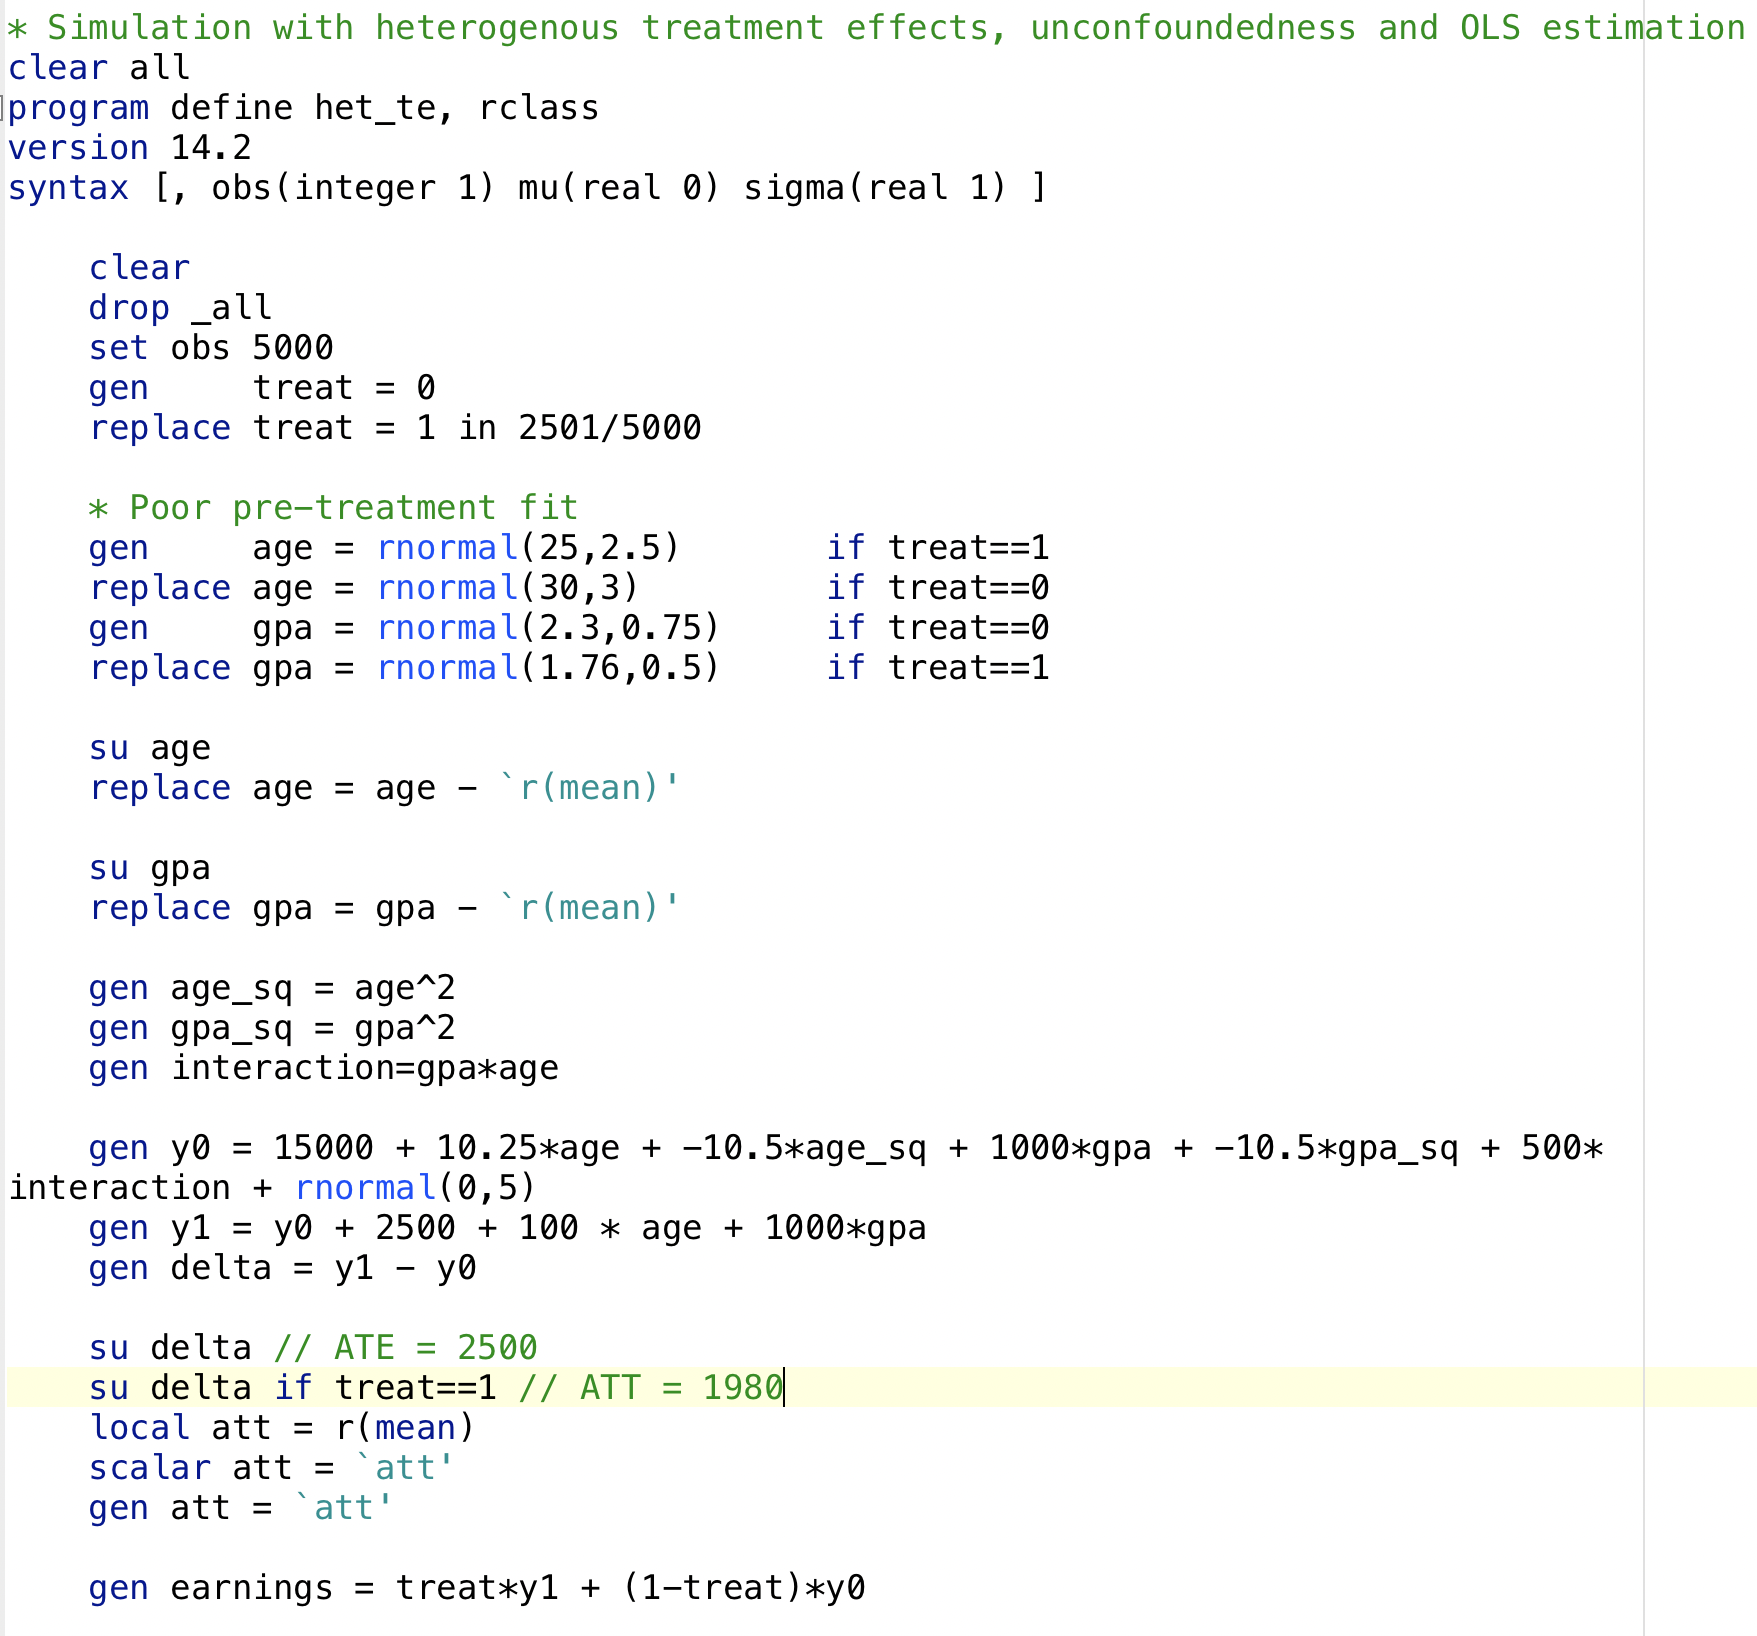
\includegraphics[scale=0.27]{./lecture_includes/stata_matching_code}
\end{figure}

\end{frame}

\begin{frame}{Parameters}

\begin{itemize}

\item We have two parameters: the ATE is \$2500 but the ATT is \$1980
\item What is the specification for each of them?
\item Let's look at what people usually do
\item 1,000 simulations of DGP with regression estimates plotting coefficient on treatment dummy: first with just age and GPA, second with the precise model used for $Y^0$ (but not $Y^1$)

\end{itemize}

\end{frame}


\begin{frame}{Constant Treatment Effects and Linearity}

\begin{figure}[!t]\centering
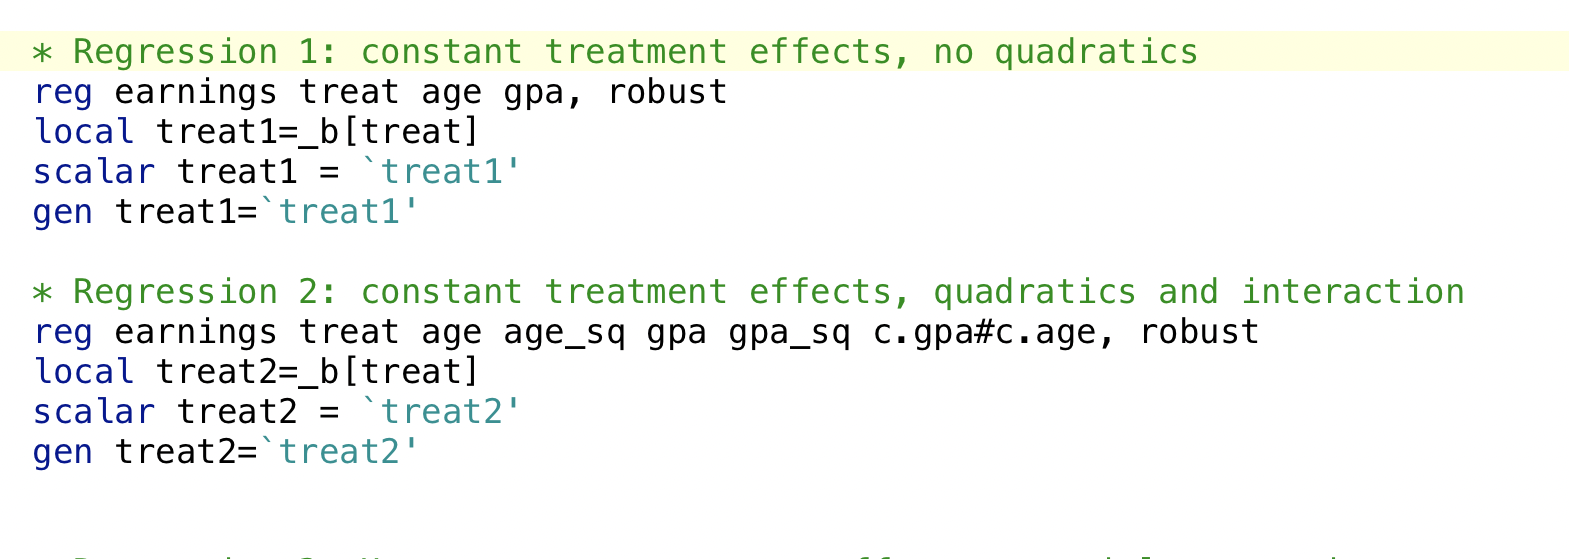
\includegraphics[scale=0.45]{./lecture_includes/stata_reg_constant}
\end{figure}

\end{frame}


\begin{frame}{Coefficient on Treatment Dummy is Wrong}

\begin{figure}[!t]\centering
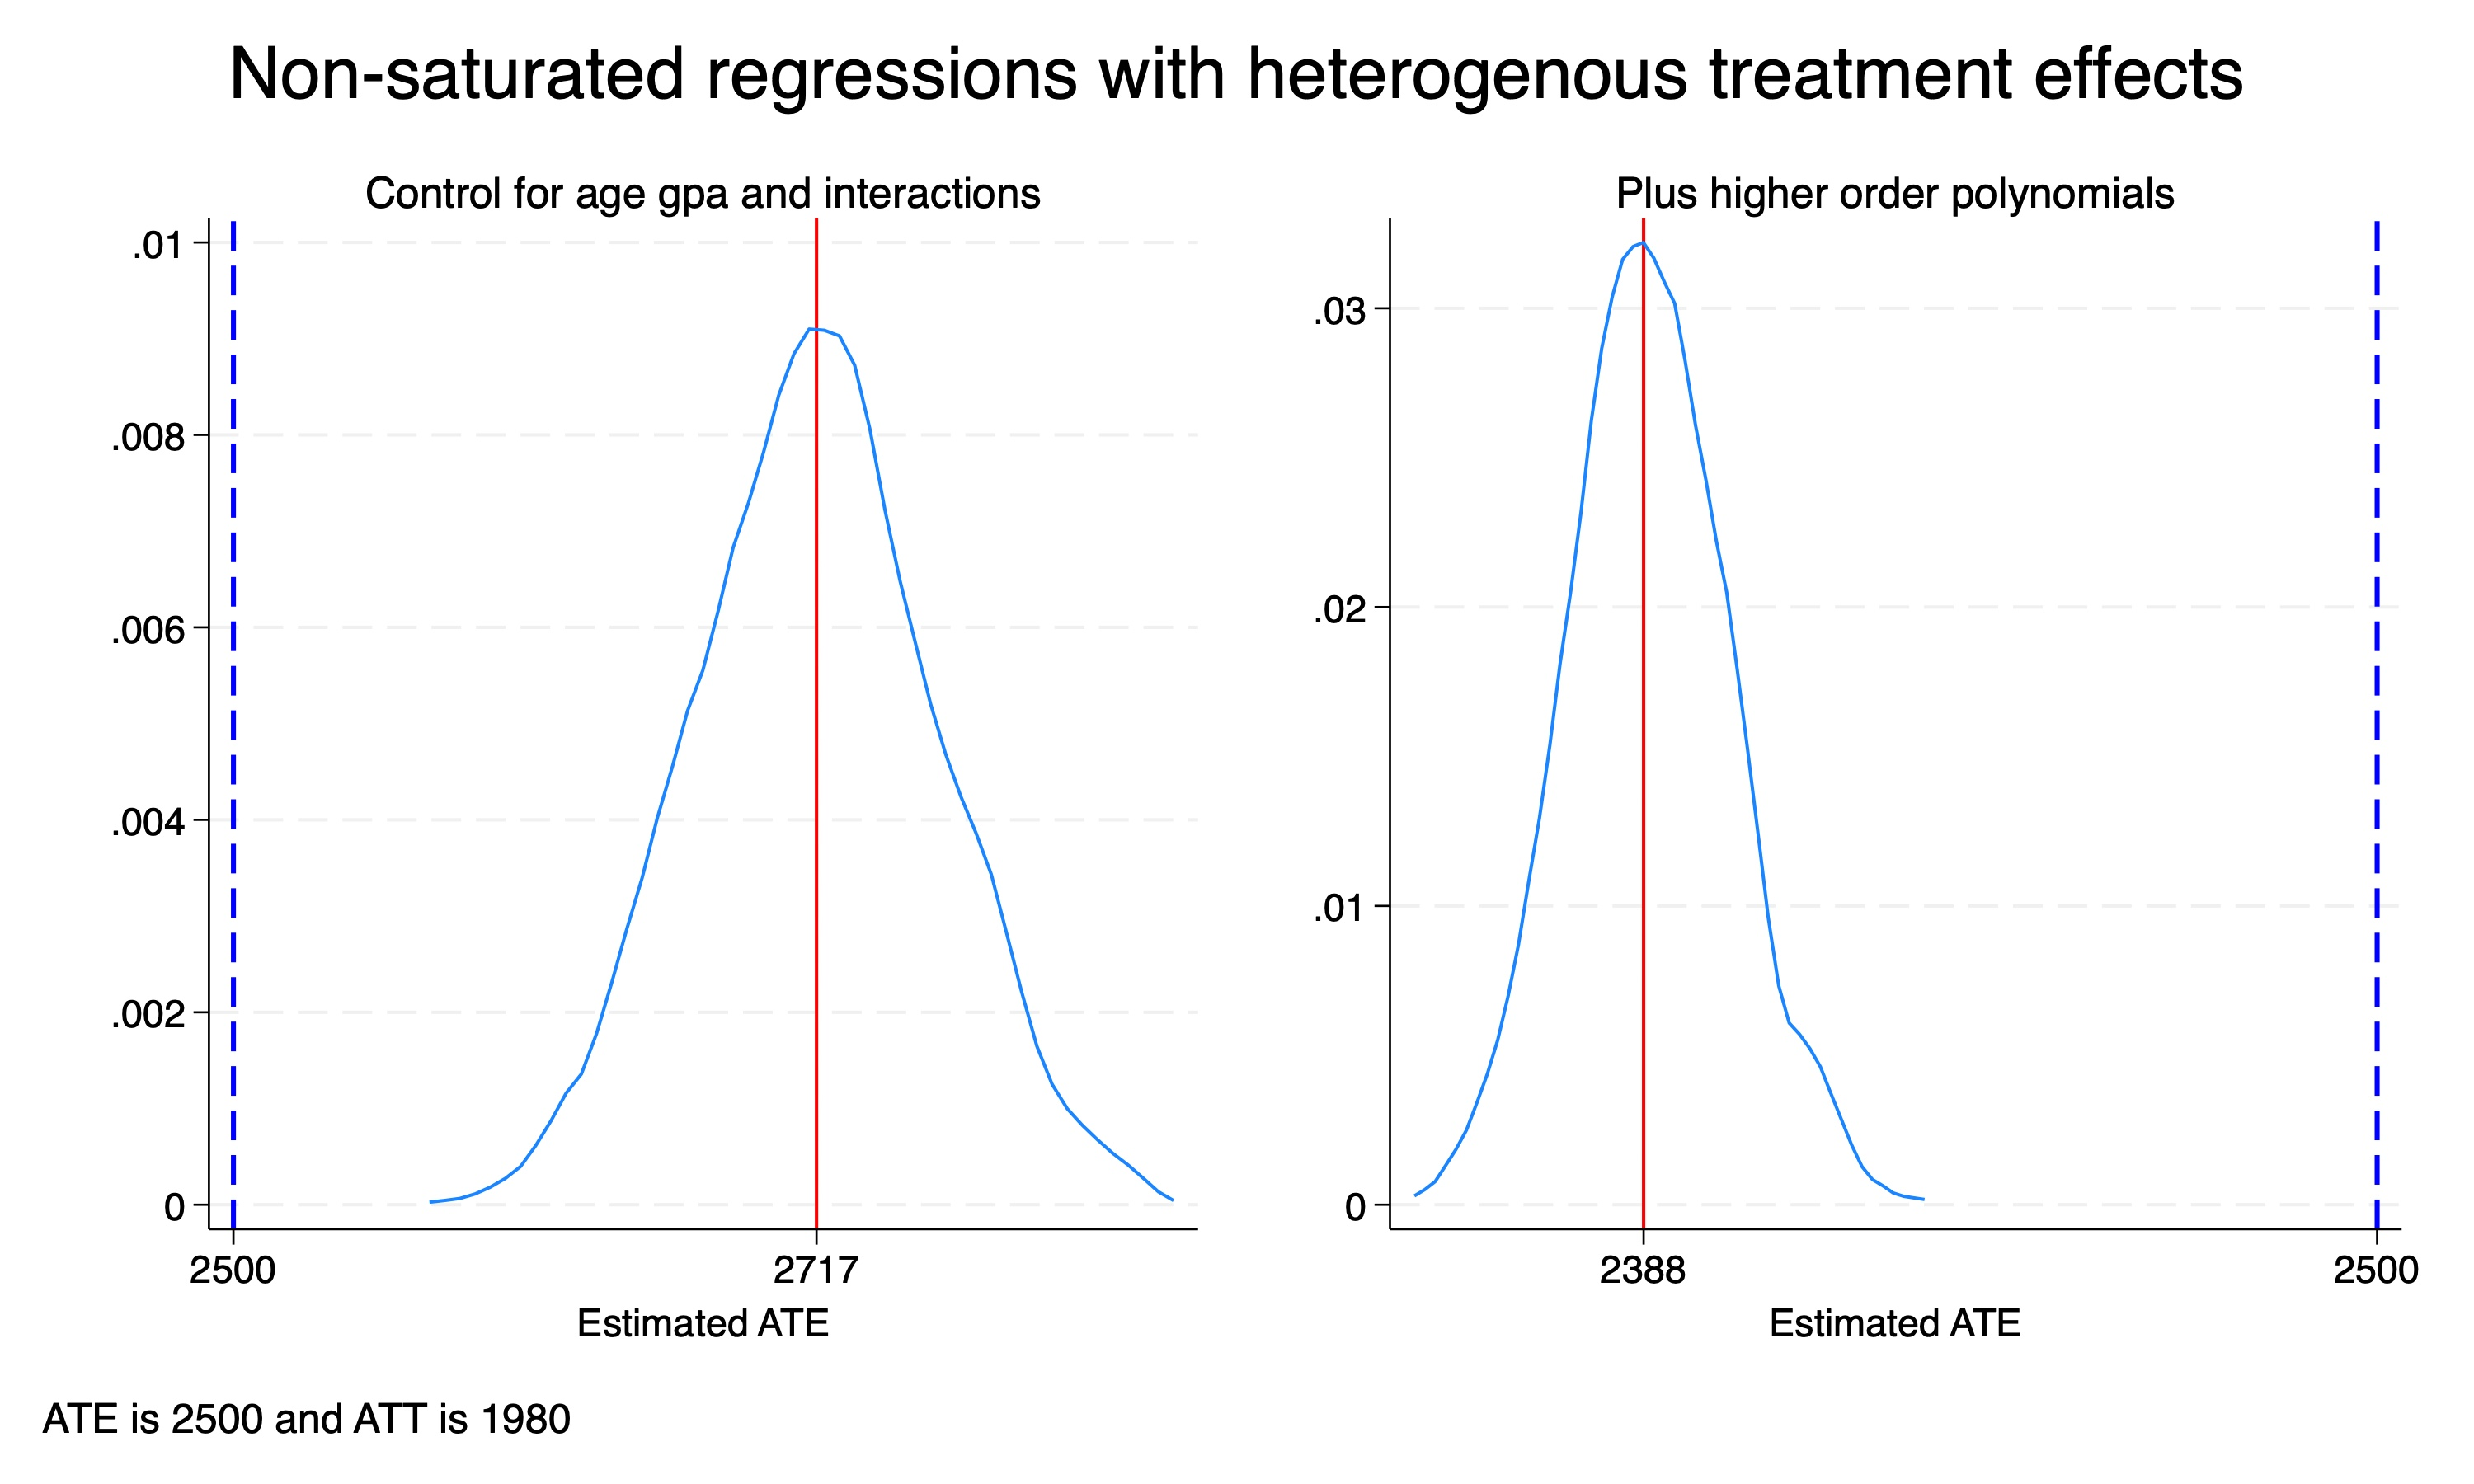
\includegraphics[scale=0.1]{./lecture_includes/combined_kernels.jpg}
\end{figure}

\end{frame}

\begin{frame}{Commentary}

\begin{itemize}

\item Three ifs and a then:

	\begin{itemize}
	\item \emph{If} unconfoundedness held, and 
	\item \emph{if} the potential outcome model was linear, and
	\item  \emph{if} the treatment effect had been homogenous with respect to age and GPA, 
	\item \emph{then} the coefficient on the treatment variable would have been the ATE 
	\end{itemize}
	
\item But it wasn't because homogeneity with respect to $X$ was not true (recall $Y(0)$ coefficients were not the same as $Y(1)$ coefficients)
\item Why were these models biased?  Didn't we have the correct specification in the second graph? 
\end{itemize}

\end{frame}

\begin{frame}{Heterogenous treatment effects}

Write down a simplified version of the DGP from the code:

\begin{eqnarray*}
Y^0_i &=& \alpha + \beta_{01} X_i + \varepsilon_i \\
Y^1_i &=& \alpha + \beta_{01} X_i + \delta D_i + \beta_{11} X_i \times D_i + \varepsilon_i
\end{eqnarray*}

\bigskip

Notice that the setup before, $X_i$ had a different effect on $Y^0$ than it did on $Y_i^1$ -- that's because of heterogenous treatment effects with respect to conditioning set. 

\end{frame}

\begin{frame}{Heterogenous treatment effects}

Take conditional expectations of the \emph{potential} outcomes:

\begin{eqnarray*}
E[Y^0_i | D_i=0, X_i] &=& \alpha + \beta_{01} E[X_i | D_i = 0, X_i] \\
E[Y^1_i | D_i=1, X_i] &=& \alpha + \beta_{01} E[X_i | D_i = 0, X_i]  \\
&& + \delta + \beta_{11} E[X_i | D_i=1,X_i]
\end{eqnarray*}

\bigskip

Average treatment effect is:  $E[Y_i^1 | D_i, X^1_i] - E[Y^0_i | D_i, X_i] $

\bigskip

\footnotesize

\begin{eqnarray*}
&=& \bigg (  \alpha + \beta_{01} E[X_i | D_i=0, X_i] + \delta + \beta_{11} E[X_i \times D_i | D_i=1,X_i] \bigg ) \\
&& -  \bigg (\alpha + \beta_{01} E[X_i  | D_i=0, X_i] \bigg ) \\
&=& \delta + \beta_{11}  E[X_i \times D_i | D_i=1] 
\end{eqnarray*}OLS model accounting for heterogeneity must be ``fully saturated''.


\end{frame}




\begin{frame}{Regression adjustment}

This implies an interacted OLS model or what Wooldridge (2010) calls regression adjustment:

\bigskip

\begin{eqnarray*}
Y_i = \alpha + \delta D_i + \beta_{01} X_i + \beta_{11} D_i \times X_i + \varepsilon_i
\end{eqnarray*}

$\widehat{\delta}$ is the ATE but the ATT is equal to $\widehat{\delta} + \widehat{\beta_{11}} E[X_i | D_i = 1]$ where $E[X_i | D_i=1]$ is the sample average of $X_i$ for the treatment group

\bigskip

We will estimate two models: (1) once with simplified but incorrectly specified saturated and (2) another with the correctly specified saturated model -- warning, it's a huge pain and you can easily mess it up even with just a few variables

\end{frame}



\begin{frame}{Misspecified Saturated OLS Regression}

\begin{figure}[!t]\centering
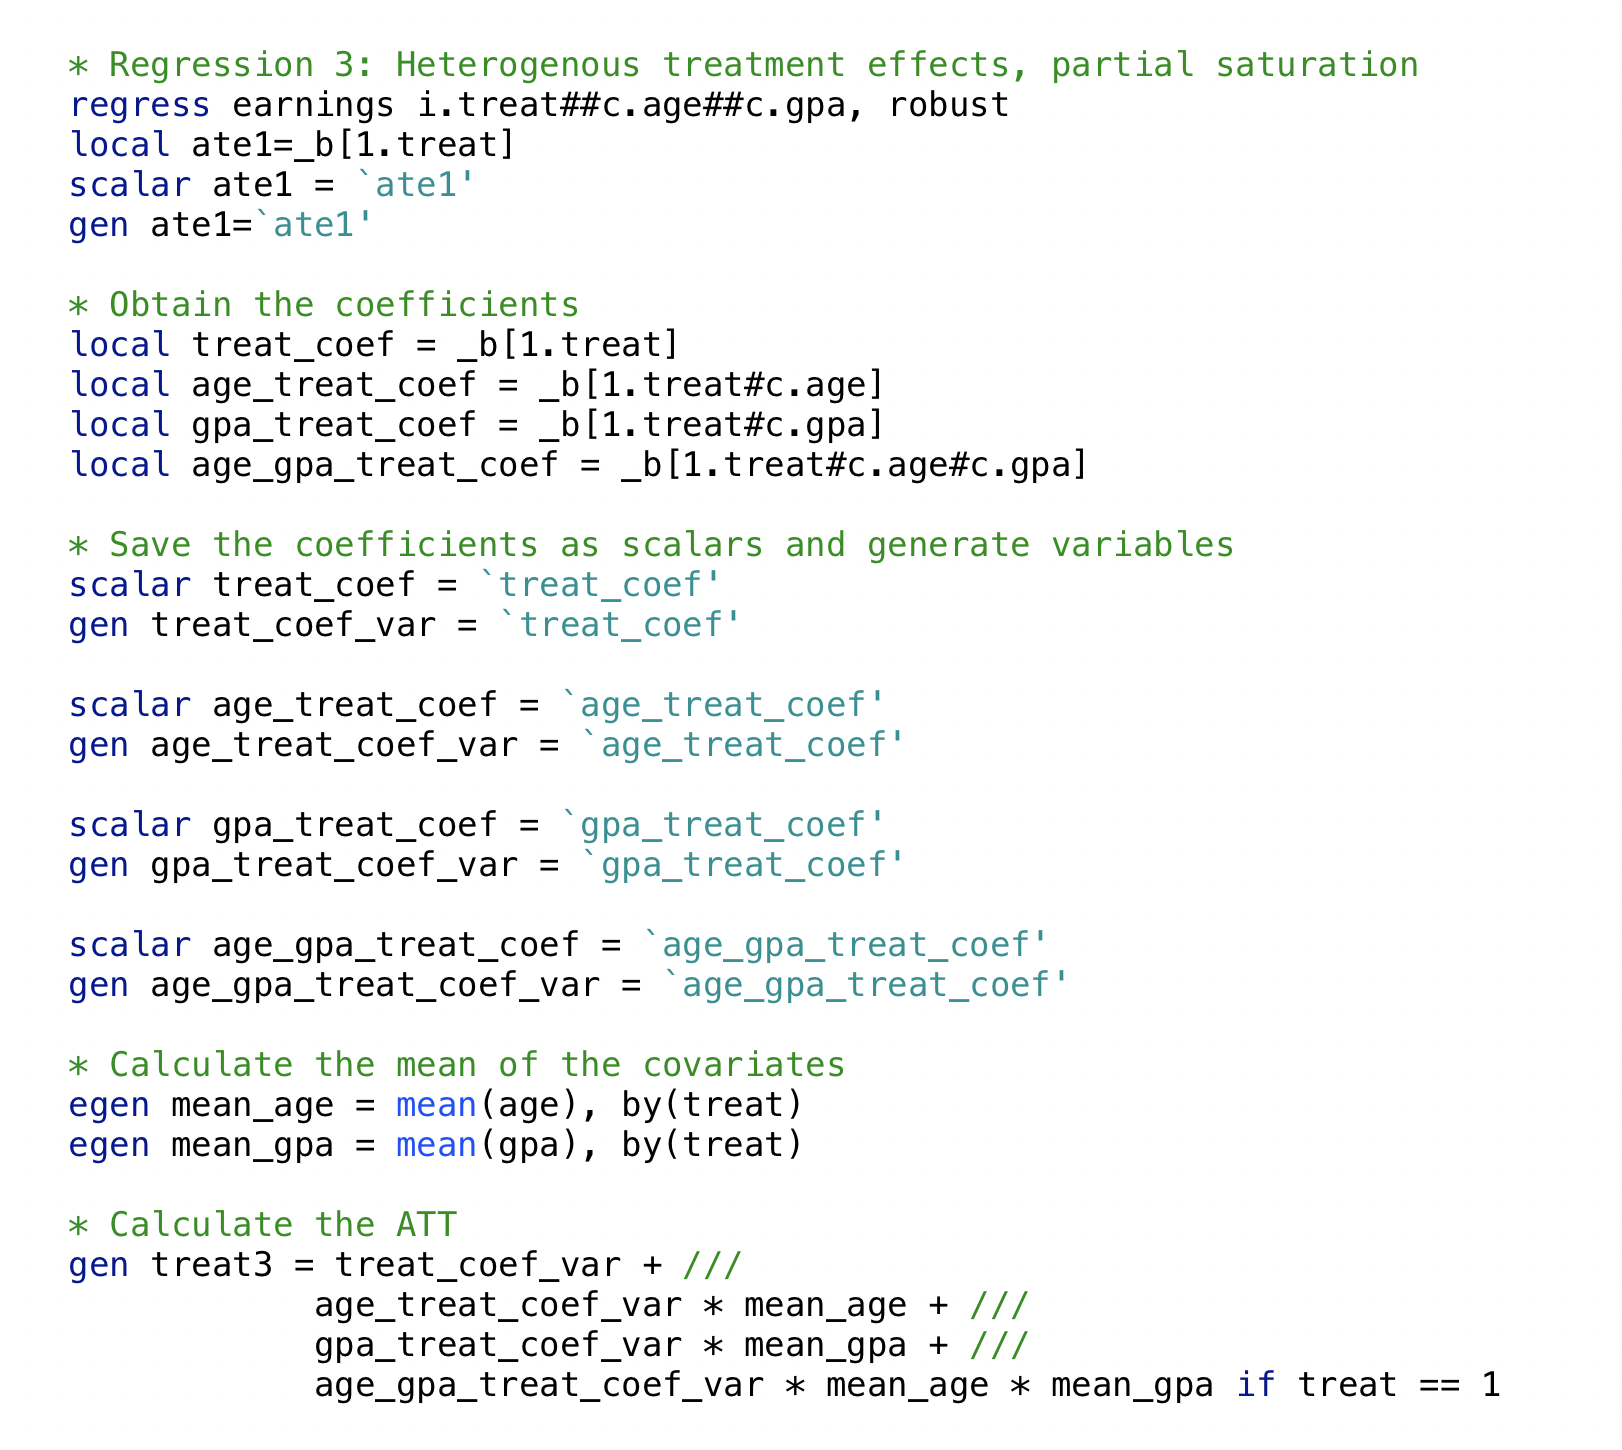
\includegraphics[scale=0.3]{./lecture_includes/saturated_reg3}
\end{figure}

\end{frame}


\begin{frame}{Misspecified Saturated OLS Regression}

\begin{figure}[!t]\centering
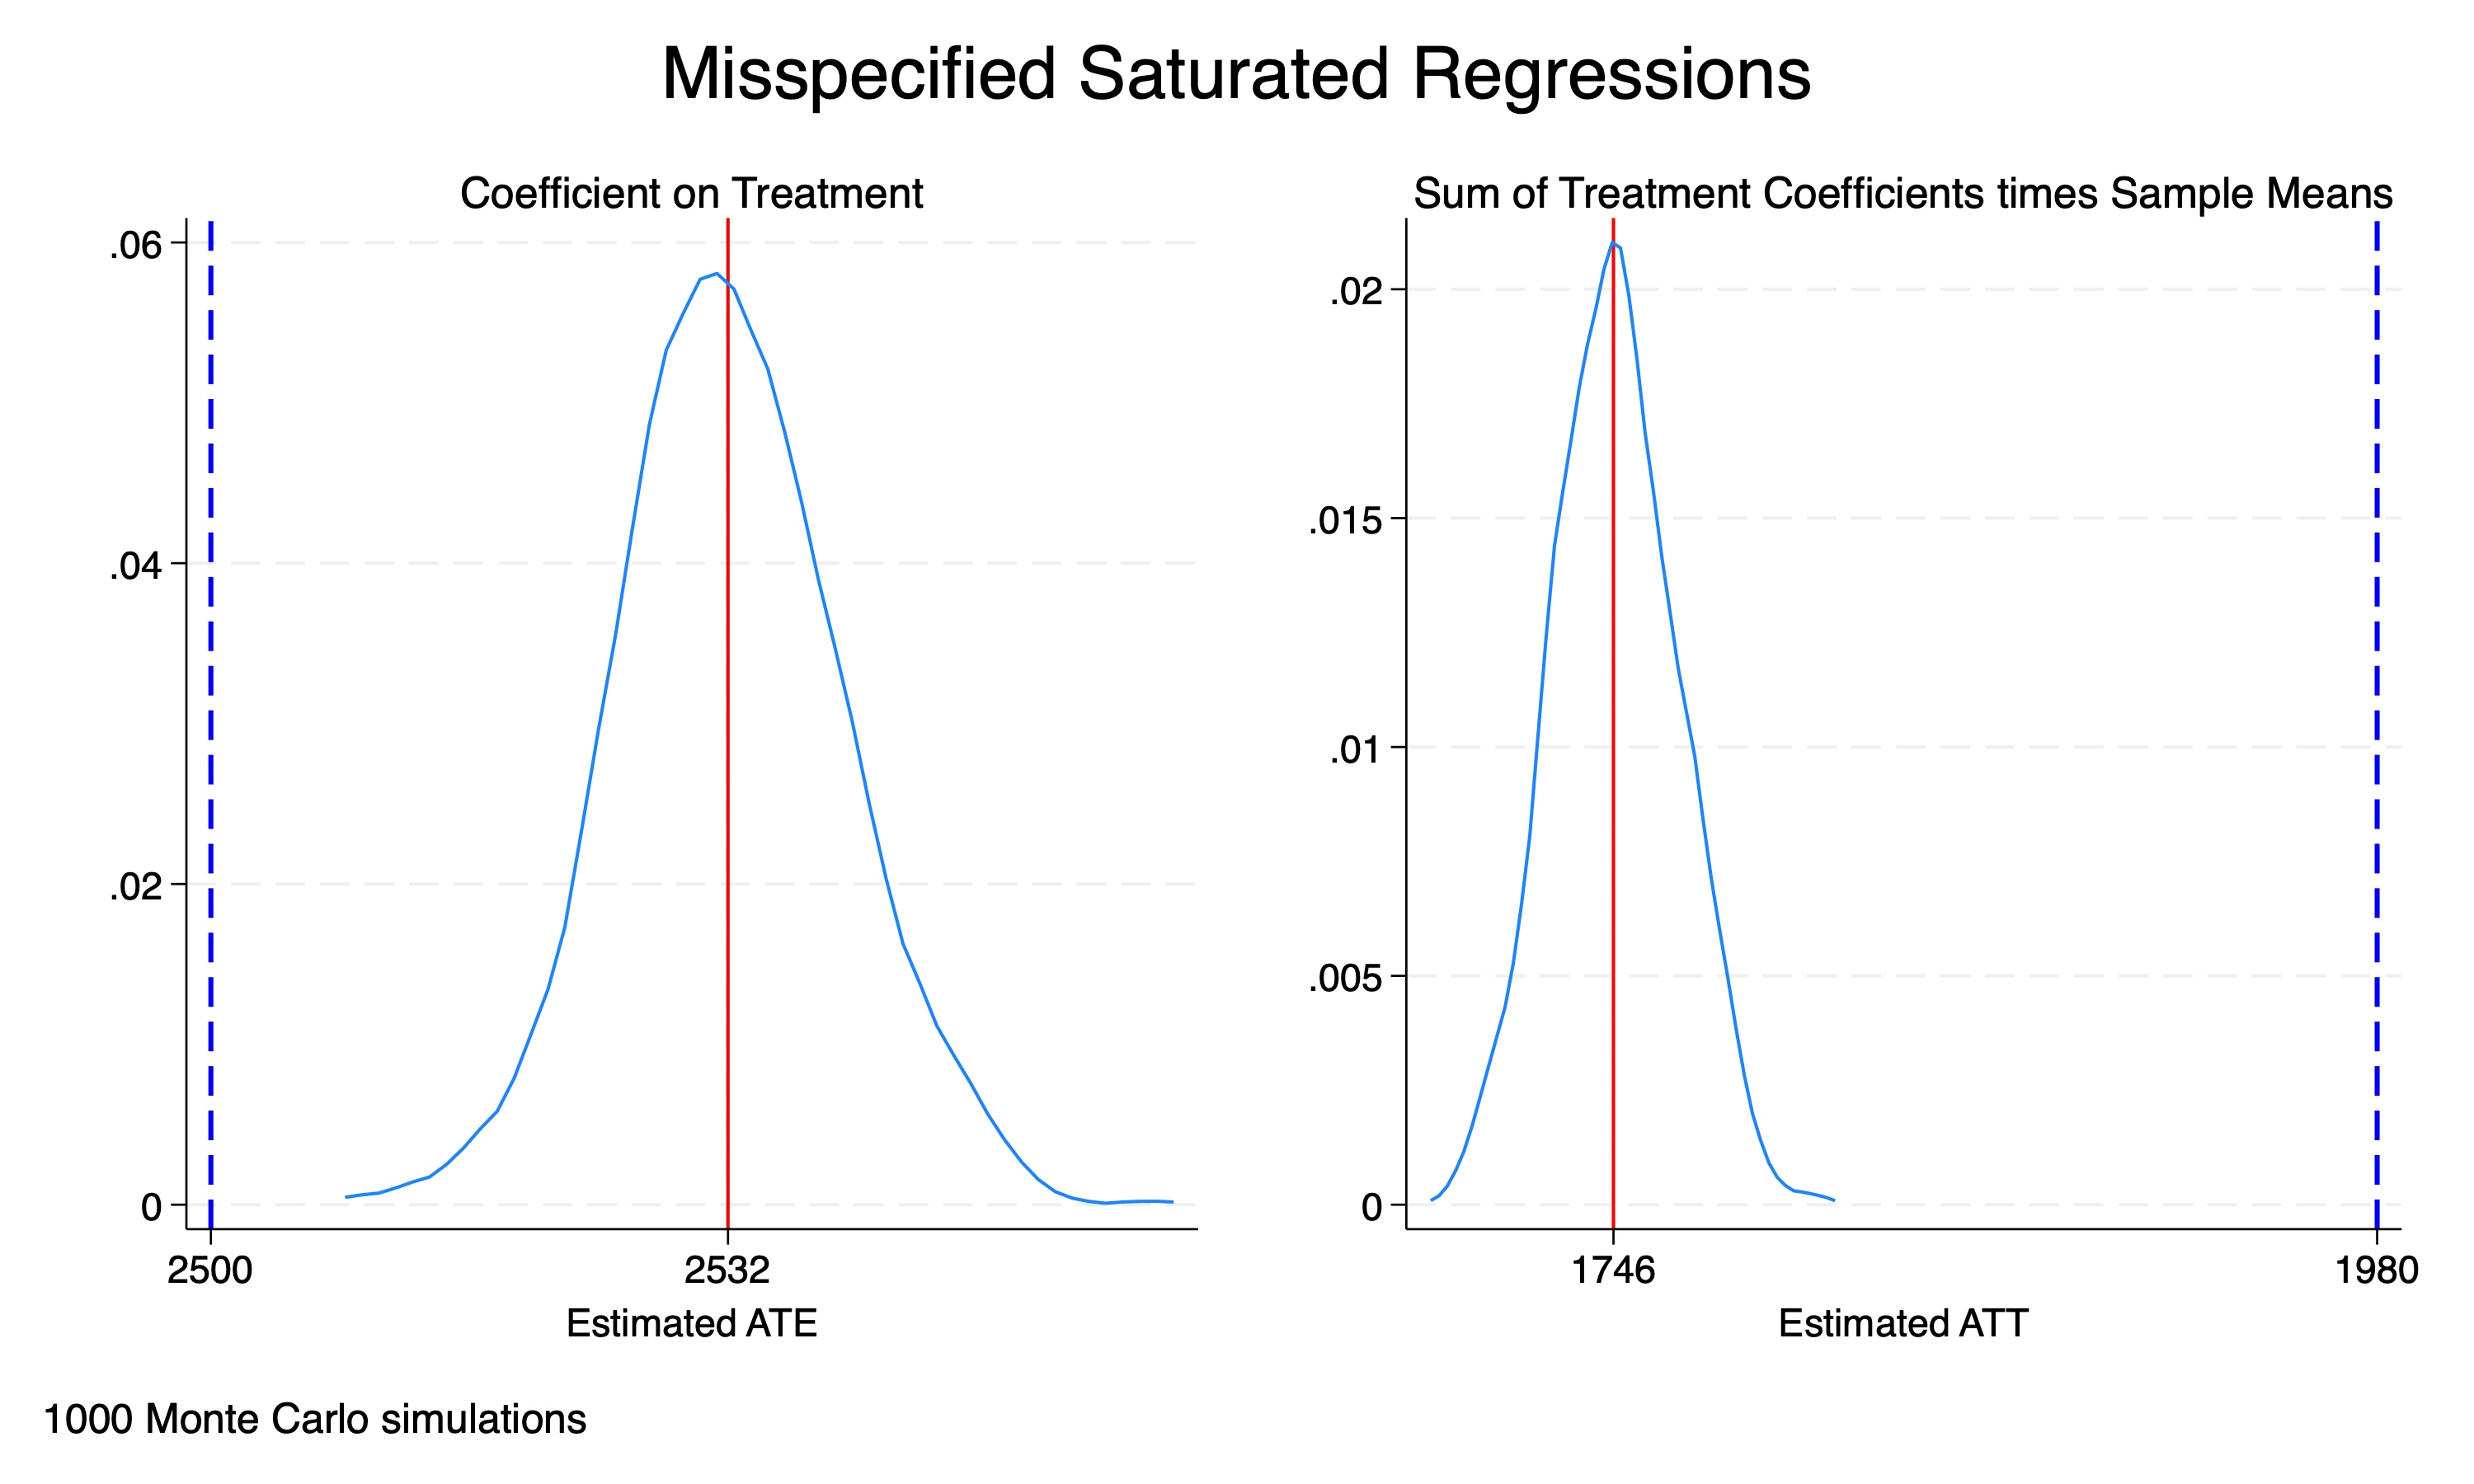
\includegraphics[scale=0.1]{./lecture_includes/combined_saturated1.jpg}
\end{figure}

\end{frame}

\begin{frame}{Comically Long Saturated OLS Regression}

\begin{figure}[!t]\centering
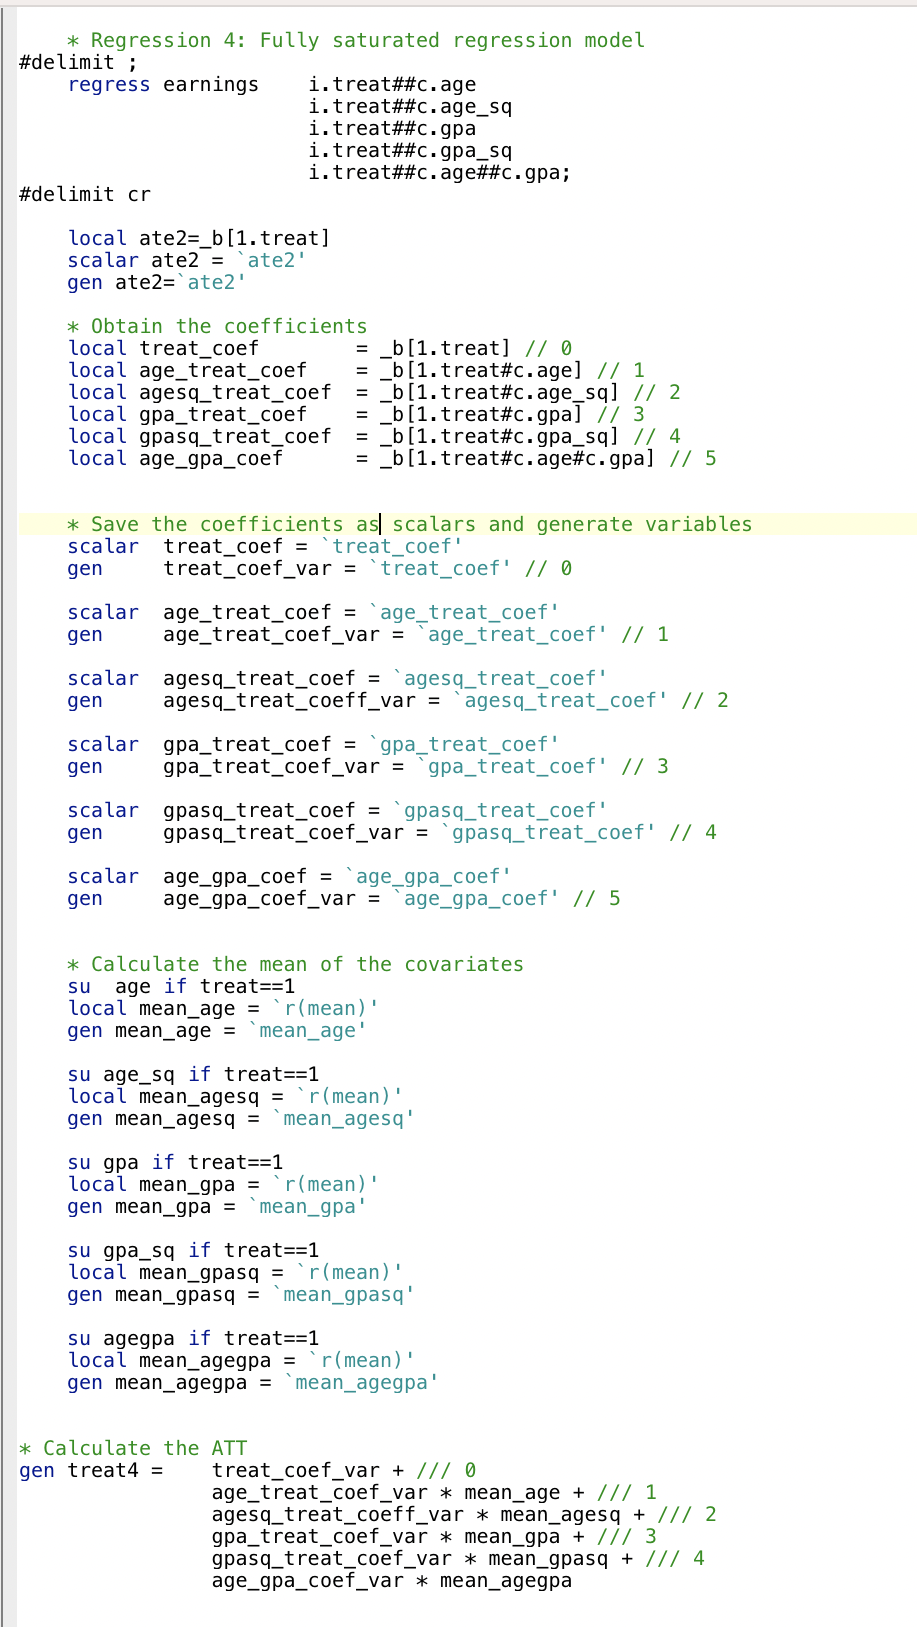
\includegraphics[scale=0.26]{./lecture_includes/stata_full_code}
\end{figure}

\end{frame}

\begin{frame}{Correctly Saturated OLS Regression}

\begin{figure}[!t]\centering
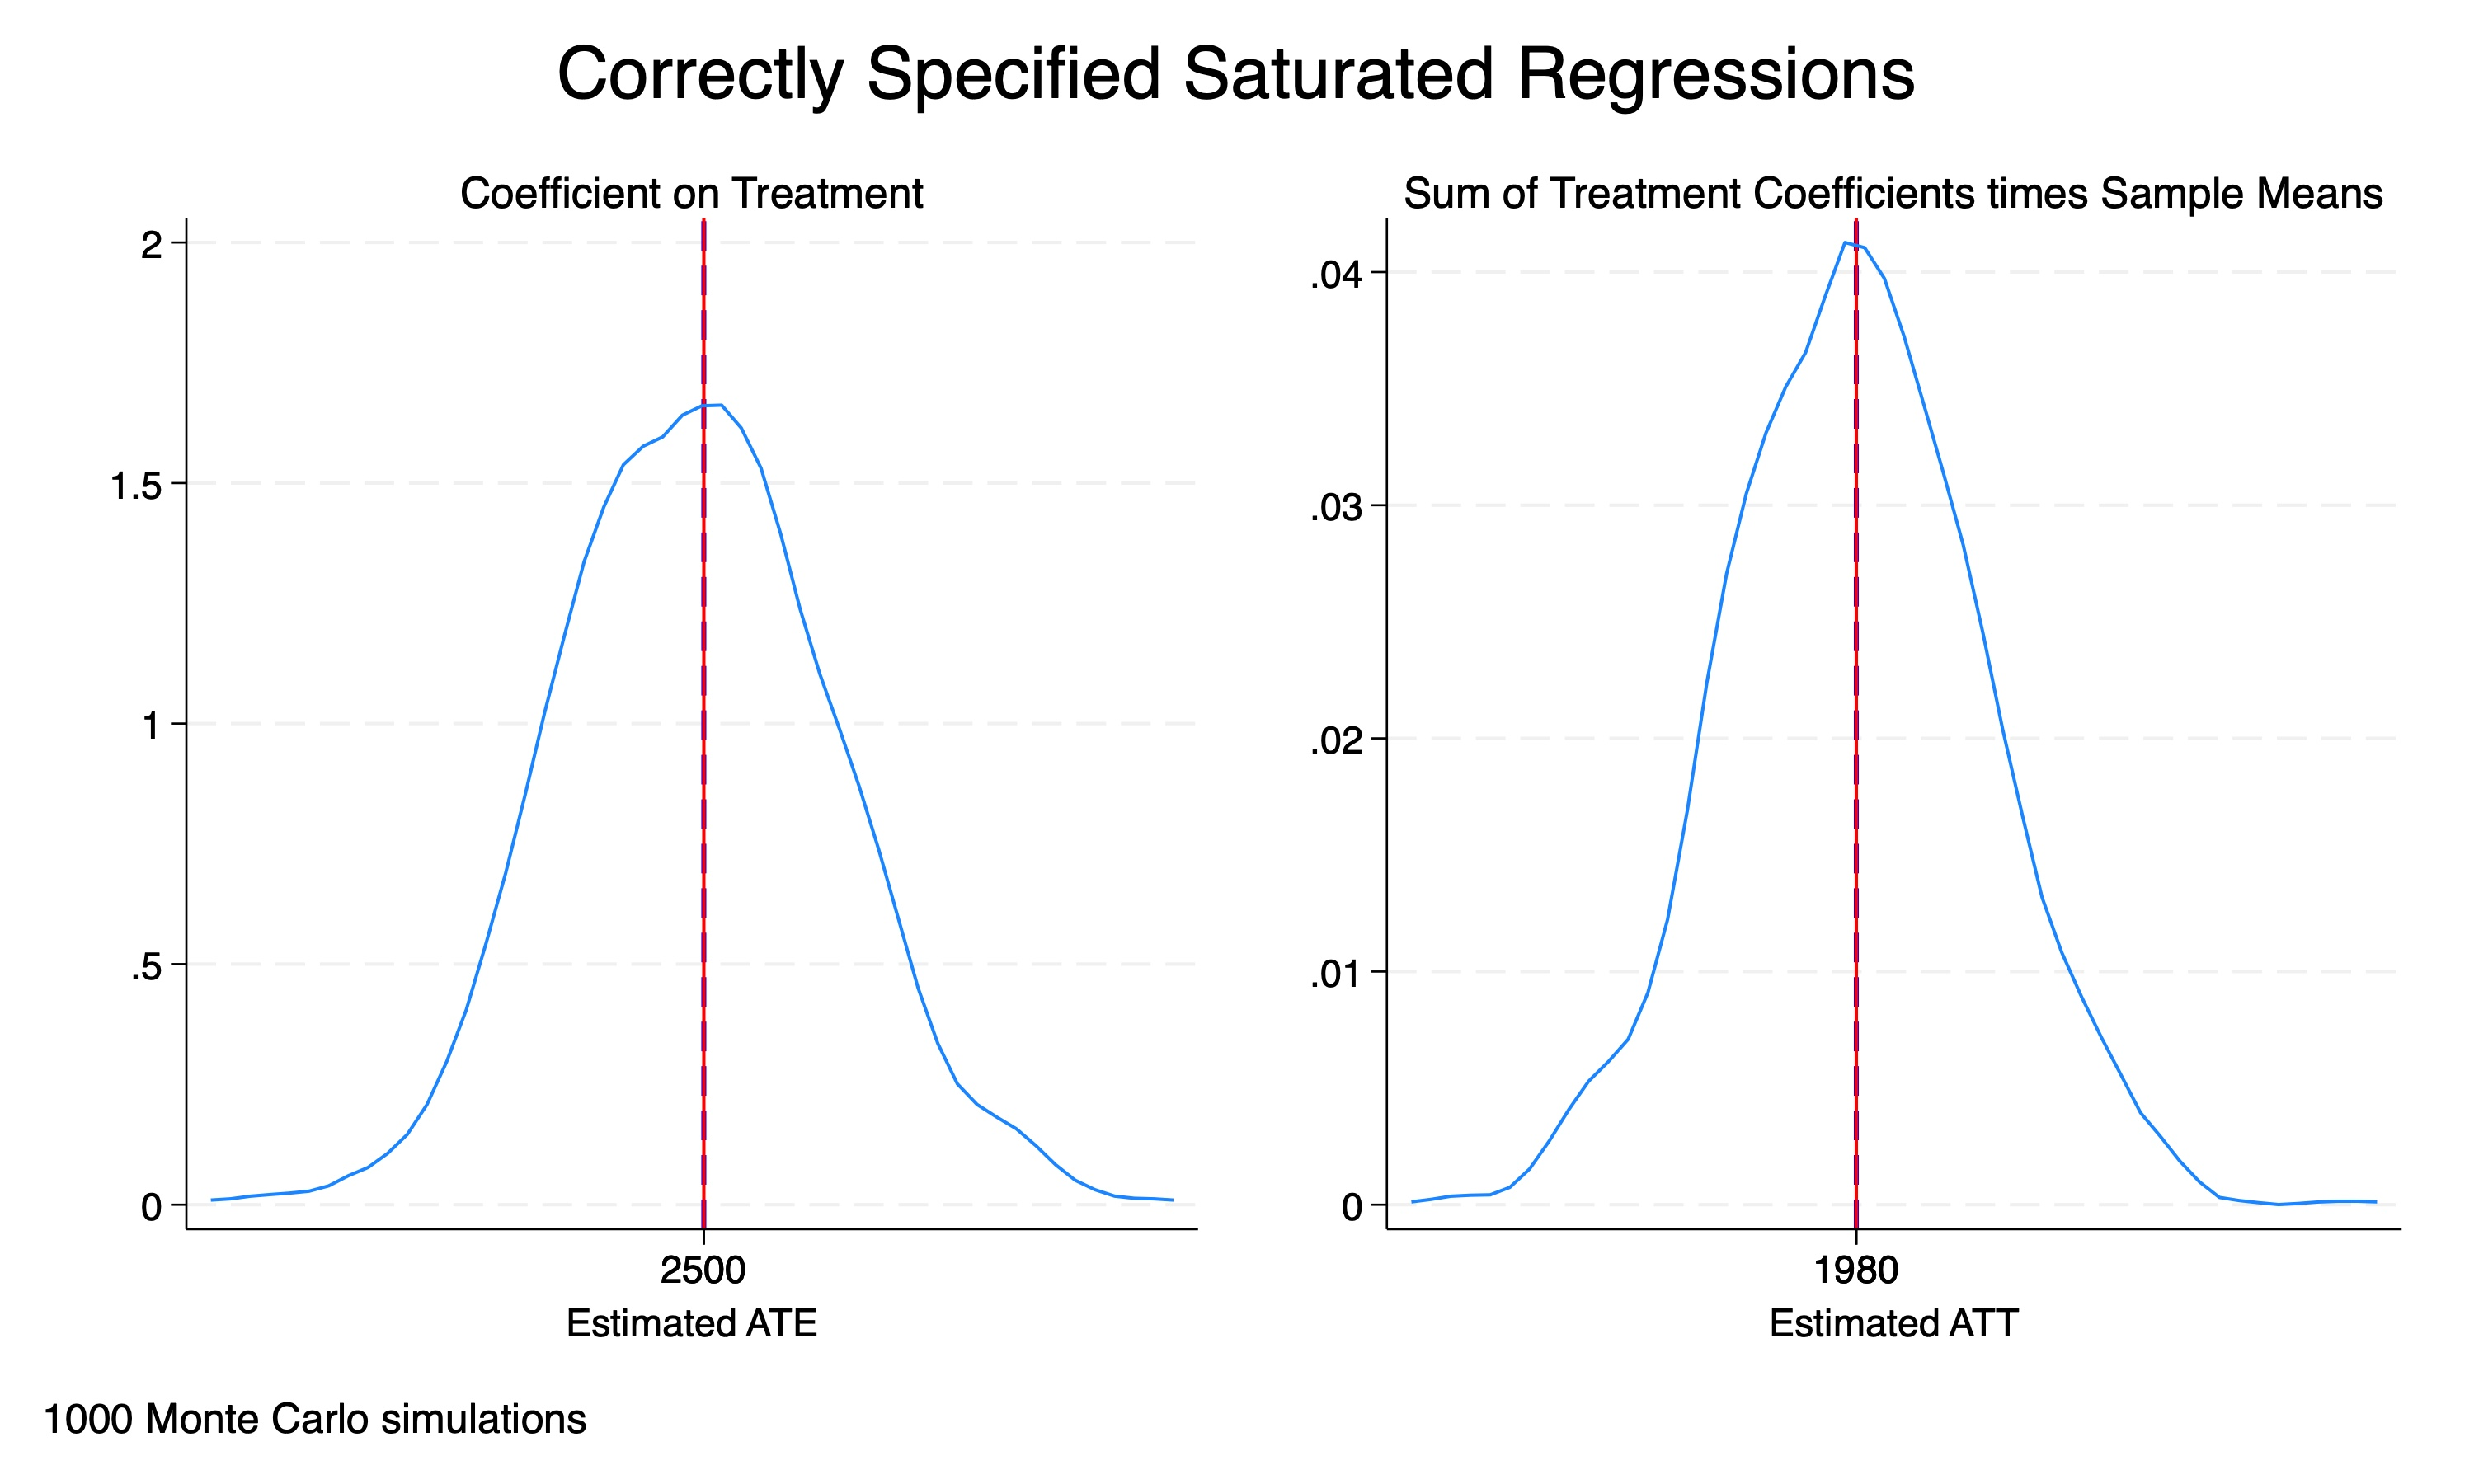
\includegraphics[scale=0.1]{./lecture_includes/combined_saturated2.jpg}
\end{figure}

\end{frame}

\begin{frame}{Regression adjustment}

\begin{itemize}

\item Notice how the same regression (fully interacted) led to \emph{both} the ATE and the ATT?
\item That means if you don't state ahead of time which parameter you want, how are you going to know how to set it up, and how will you know how to recover it?
\item Thankfully software exists that does this for you called ``regression adjustment'' by Wooldridge (2010) or Oaxaca-Blinder (Kline 2011; Graham and Pinto 2022) 
\item In Stata teffects, you can just the \texttt{ra} to get it -- see \texttt{comparison.do}

\end{itemize}

\end{frame}

\begin{frame}{Great quote}

\begin{quote}
``OLS is \dots the linear projection of Y on D and X [and] provides the best linear predictor of Y given D and X (Angrist and Pishcke 2009).  However, if our goal is to conduct causal inference, then this is not, in fact, a good reason to use this method.  OLS is `best' in predicting actual outcomes, but causal inference is about predicting [fictional potential] outcomes.  \dots In other words, OLS \dots is optimal for predicting `what is'.  Instead we are interested in predicting `what would be' if treatment were assigned differently.'' - Tymon Sloczynski, Restat 2022
\end{quote}

\end{frame}


\begin{frame}{Matching}

\begin{itemize}

\item Now let's estimate the ATT (\$1980) using nearest neighbor matching by minimizing Mahalanobis distance on age, GPA, polynomials and interaction
\item One line in Stata using \texttt{teffects} and only 1 match (variance is simple to estimate until we use matches multiple times, then the variance grows)
\item In R, the package is \texttt{Matching}, not sure in python
\end{itemize}

\end{frame}


\begin{frame}{Matching Estimation}

\begin{figure}[!t]\centering
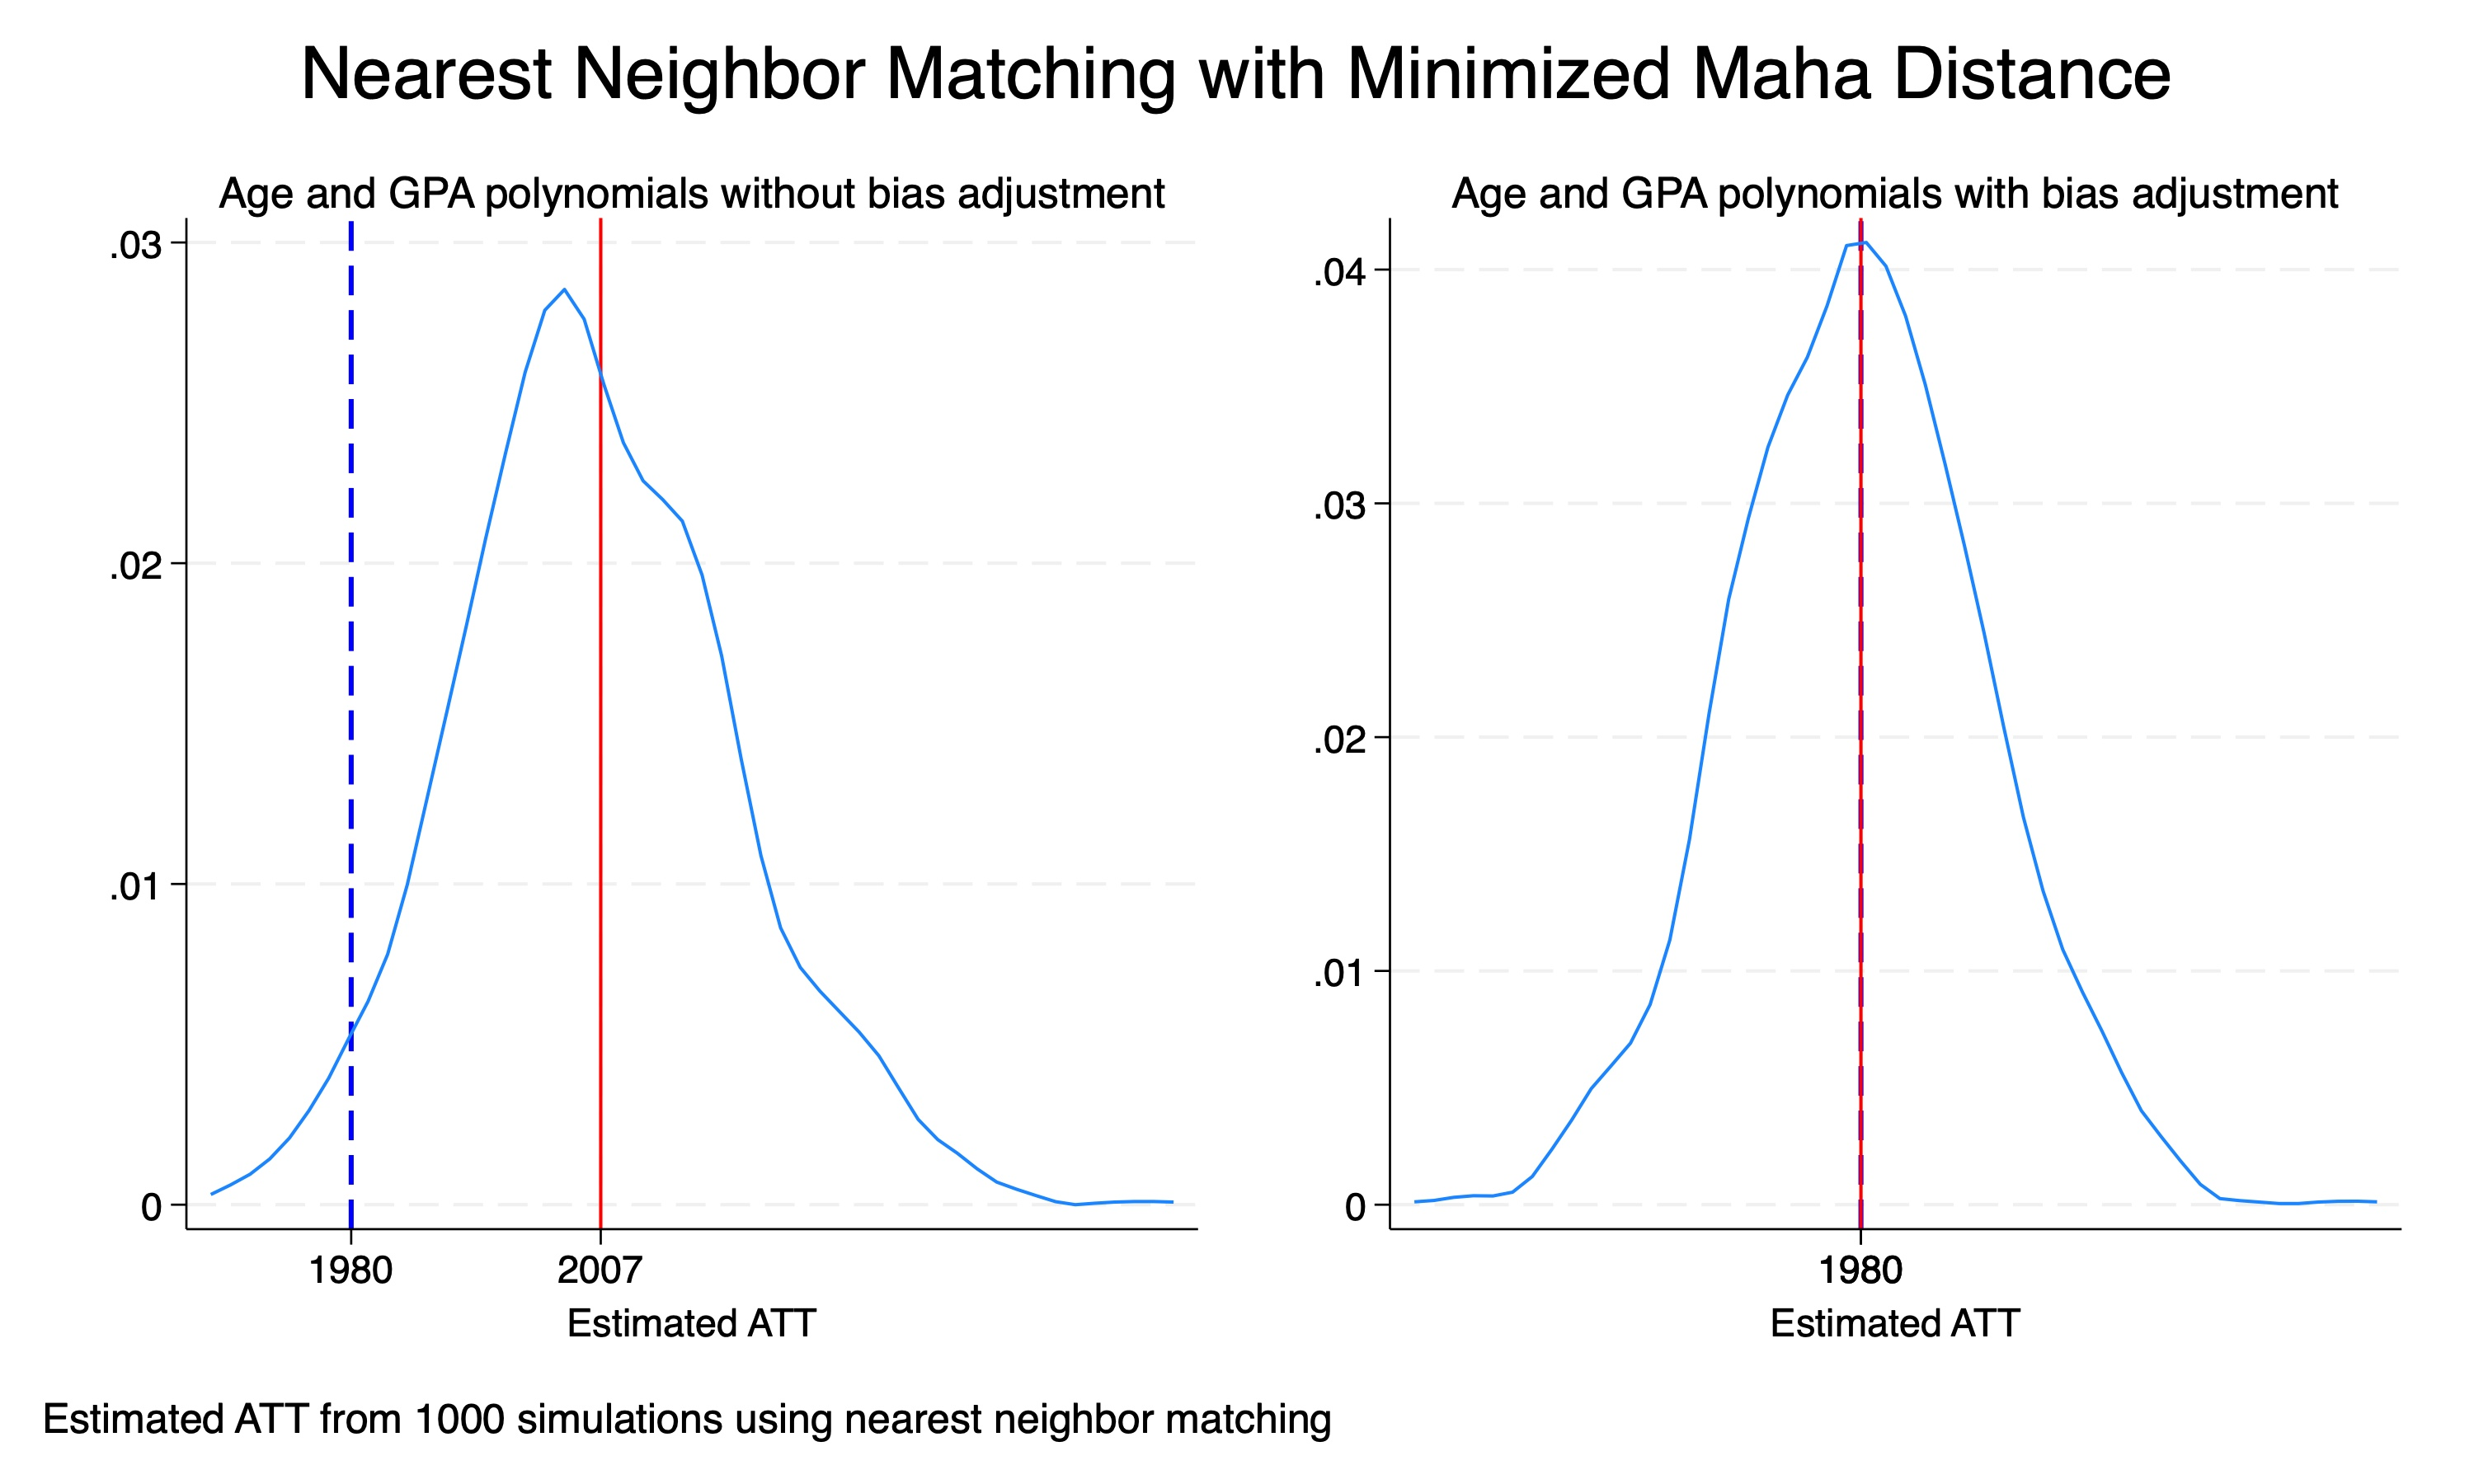
\includegraphics[scale=0.1]{./lecture_includes/combined_kernels_maha.jpg}
\end{figure}

\end{frame}

\begin{frame}{Commentary}

\begin{itemize}

\item Technically I was only ``fully interacting'' -- full saturation would be to interact the treatment dummy with every value of the covariates yielding a huge number of parameters likely that cannot be estimated
\item Regression adjustment within -teffects- will do this for you
\item But note, with heterogeneity you have to use the fully saturated model (I just hadn't dummied every value of the covariates) to get both the ATE and the ATT
\item Otherwise you are imposing strong and unnecessary assumptions on the data that the treatment effects are the same for all values of $X$ and constant treatment effects so that the single coefficient is the ATE and the ATT

\end{itemize}

\end{frame}

\begin{frame}{Misspecified functional form regression visual}

  \begin{figure}
    
\includegraphics[scale=0.17]{./lecture_includes/regression_linearity.png}
  \end{figure}
  
Using our medieval castle example, if you have the wrong functional form, then regression won't hit.

\end{frame}


\begin{frame}{Nonlinear DGP}

\begin{itemize}

\item We've seen what happens if there's heterogenous treatment effects with respect to covariates
\item But this was resolvable with ``full interaction'' or ``regression adjustment''
\item But Imbens and Rubin (2015) noted that exogeneity also implied functional forms, namely linearity
\item Let's examine this now using a very unusual DGP using \texttt{nonlinear\_matching.do}

\end{itemize}

\end{frame}




\begin{frame}{Nonlinear DGP}

\begin{figure}[!t]\centering
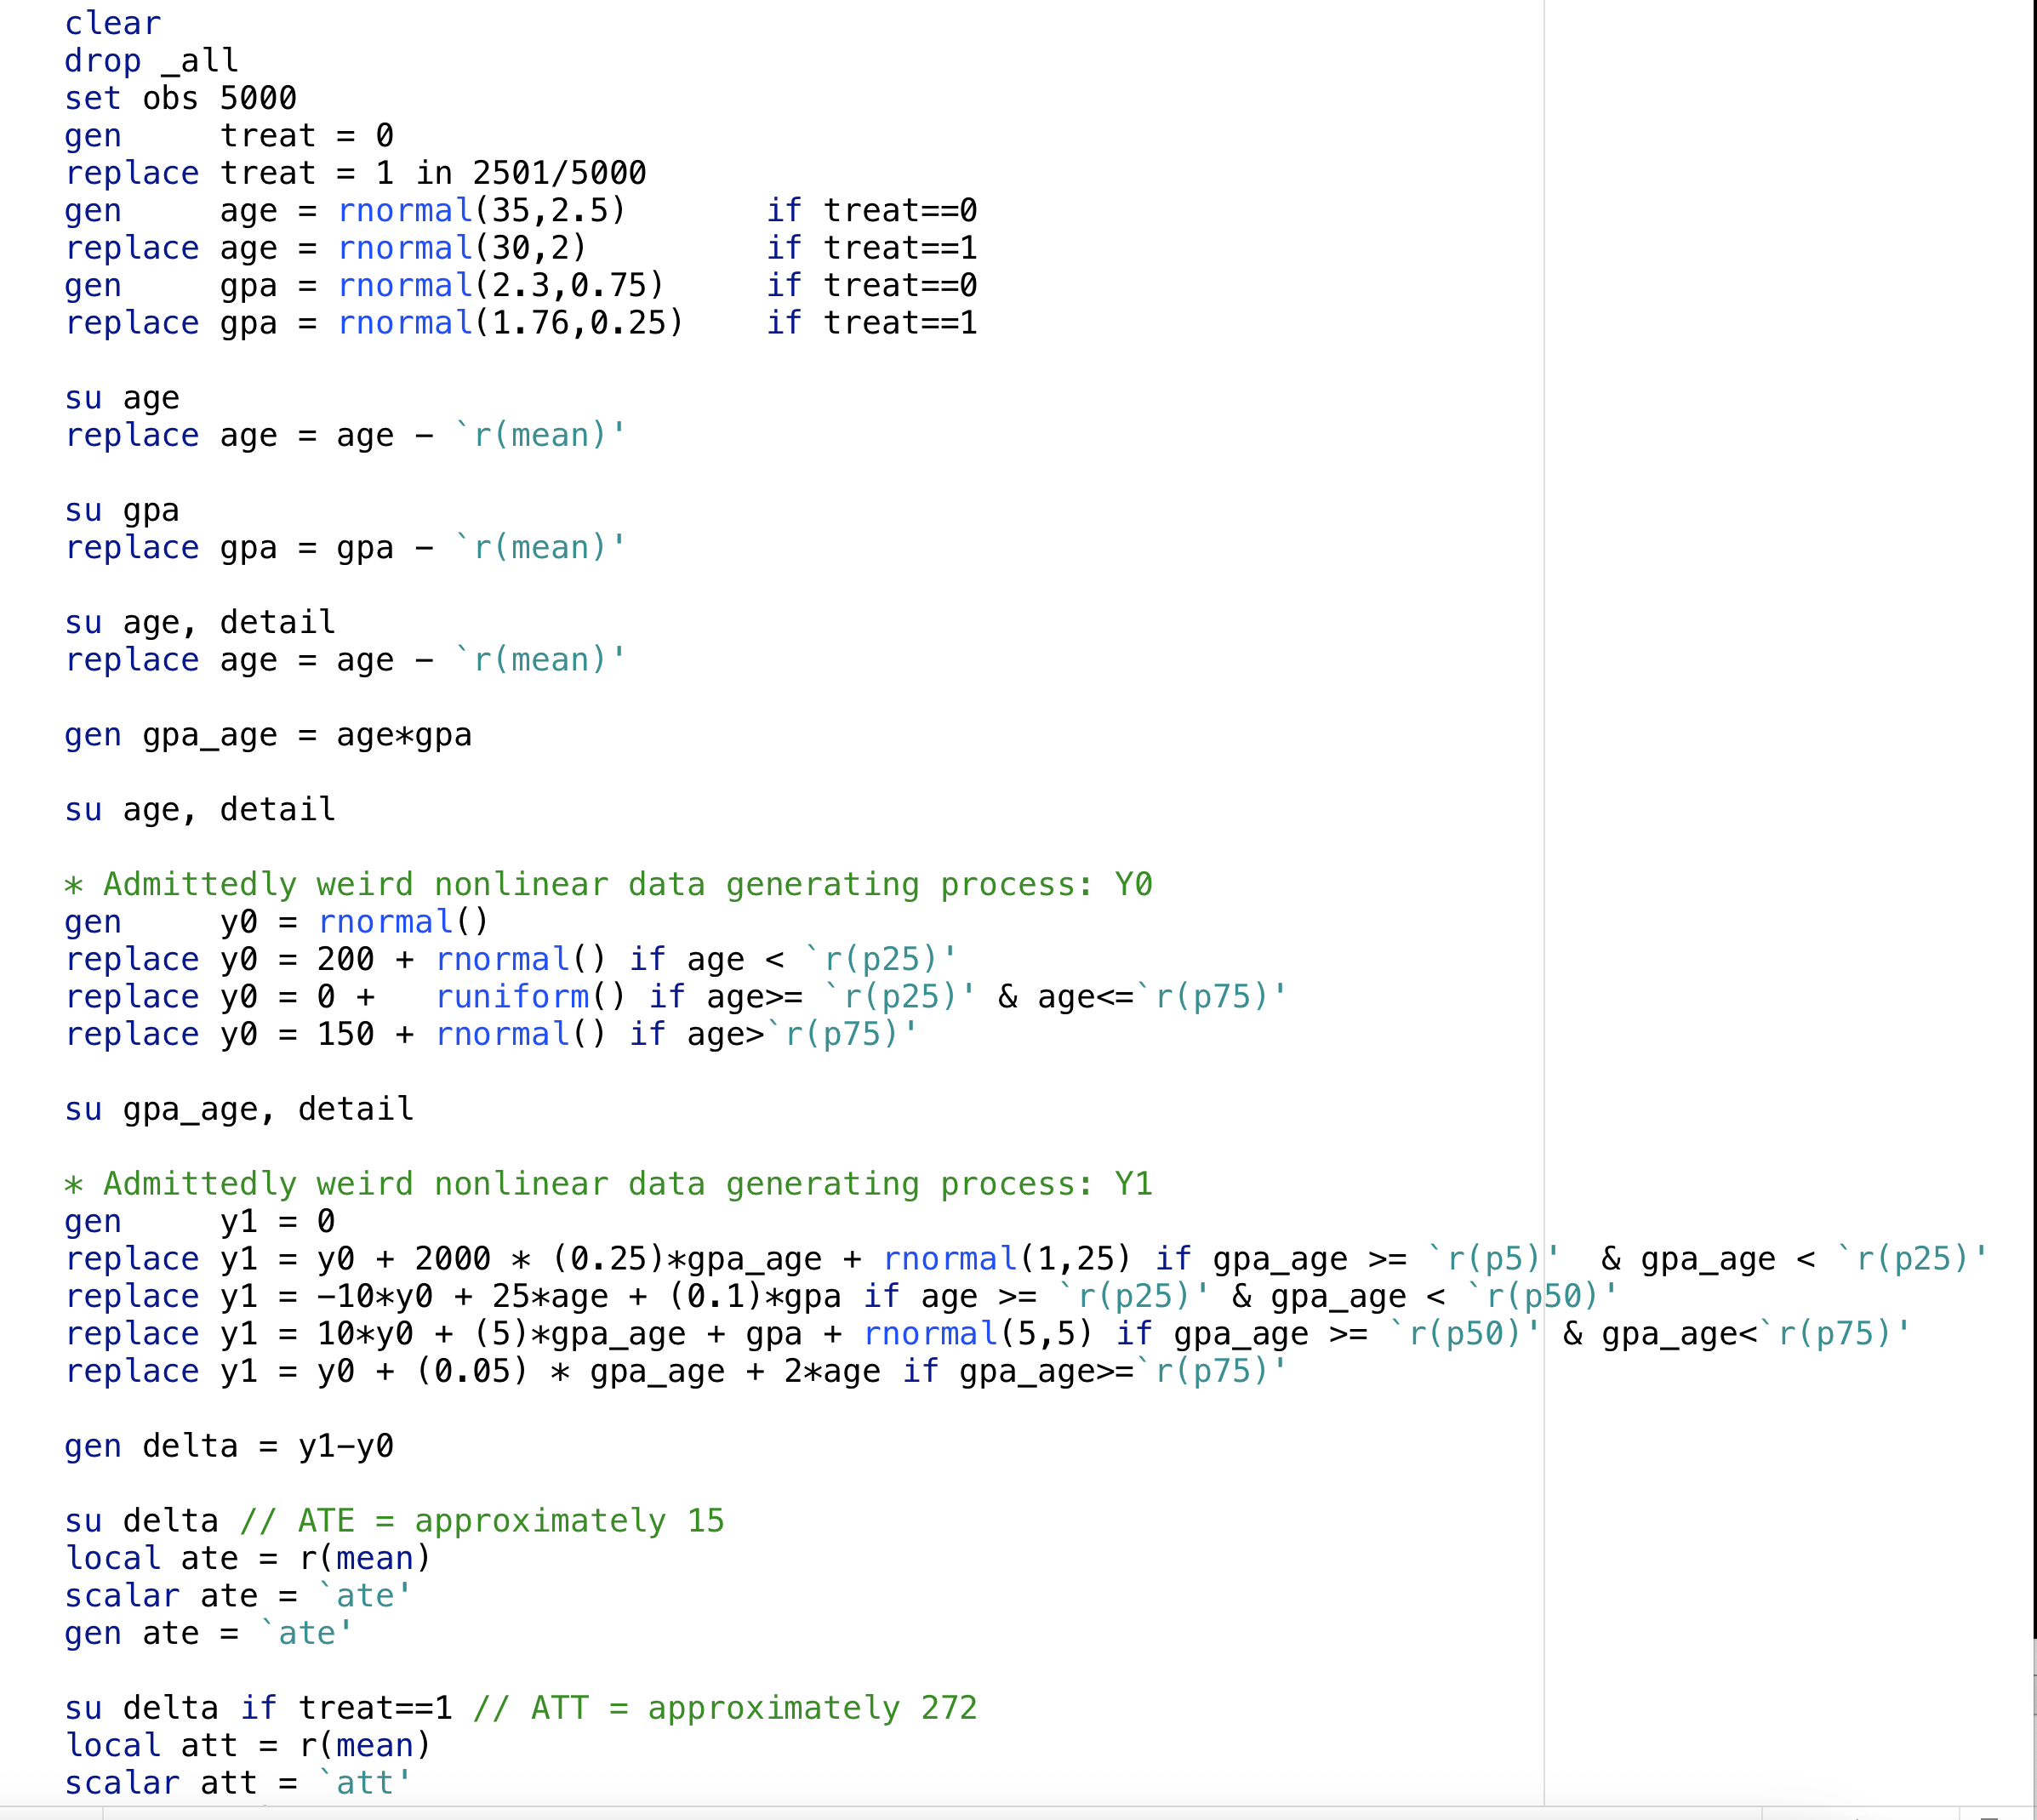
\includegraphics[scale=0.21]{./lecture_includes/nonlinear_code}
\end{figure}

\end{frame}

\begin{frame}{Nonlinear DGP, OLS with RA}

\begin{figure}[!t]\centering
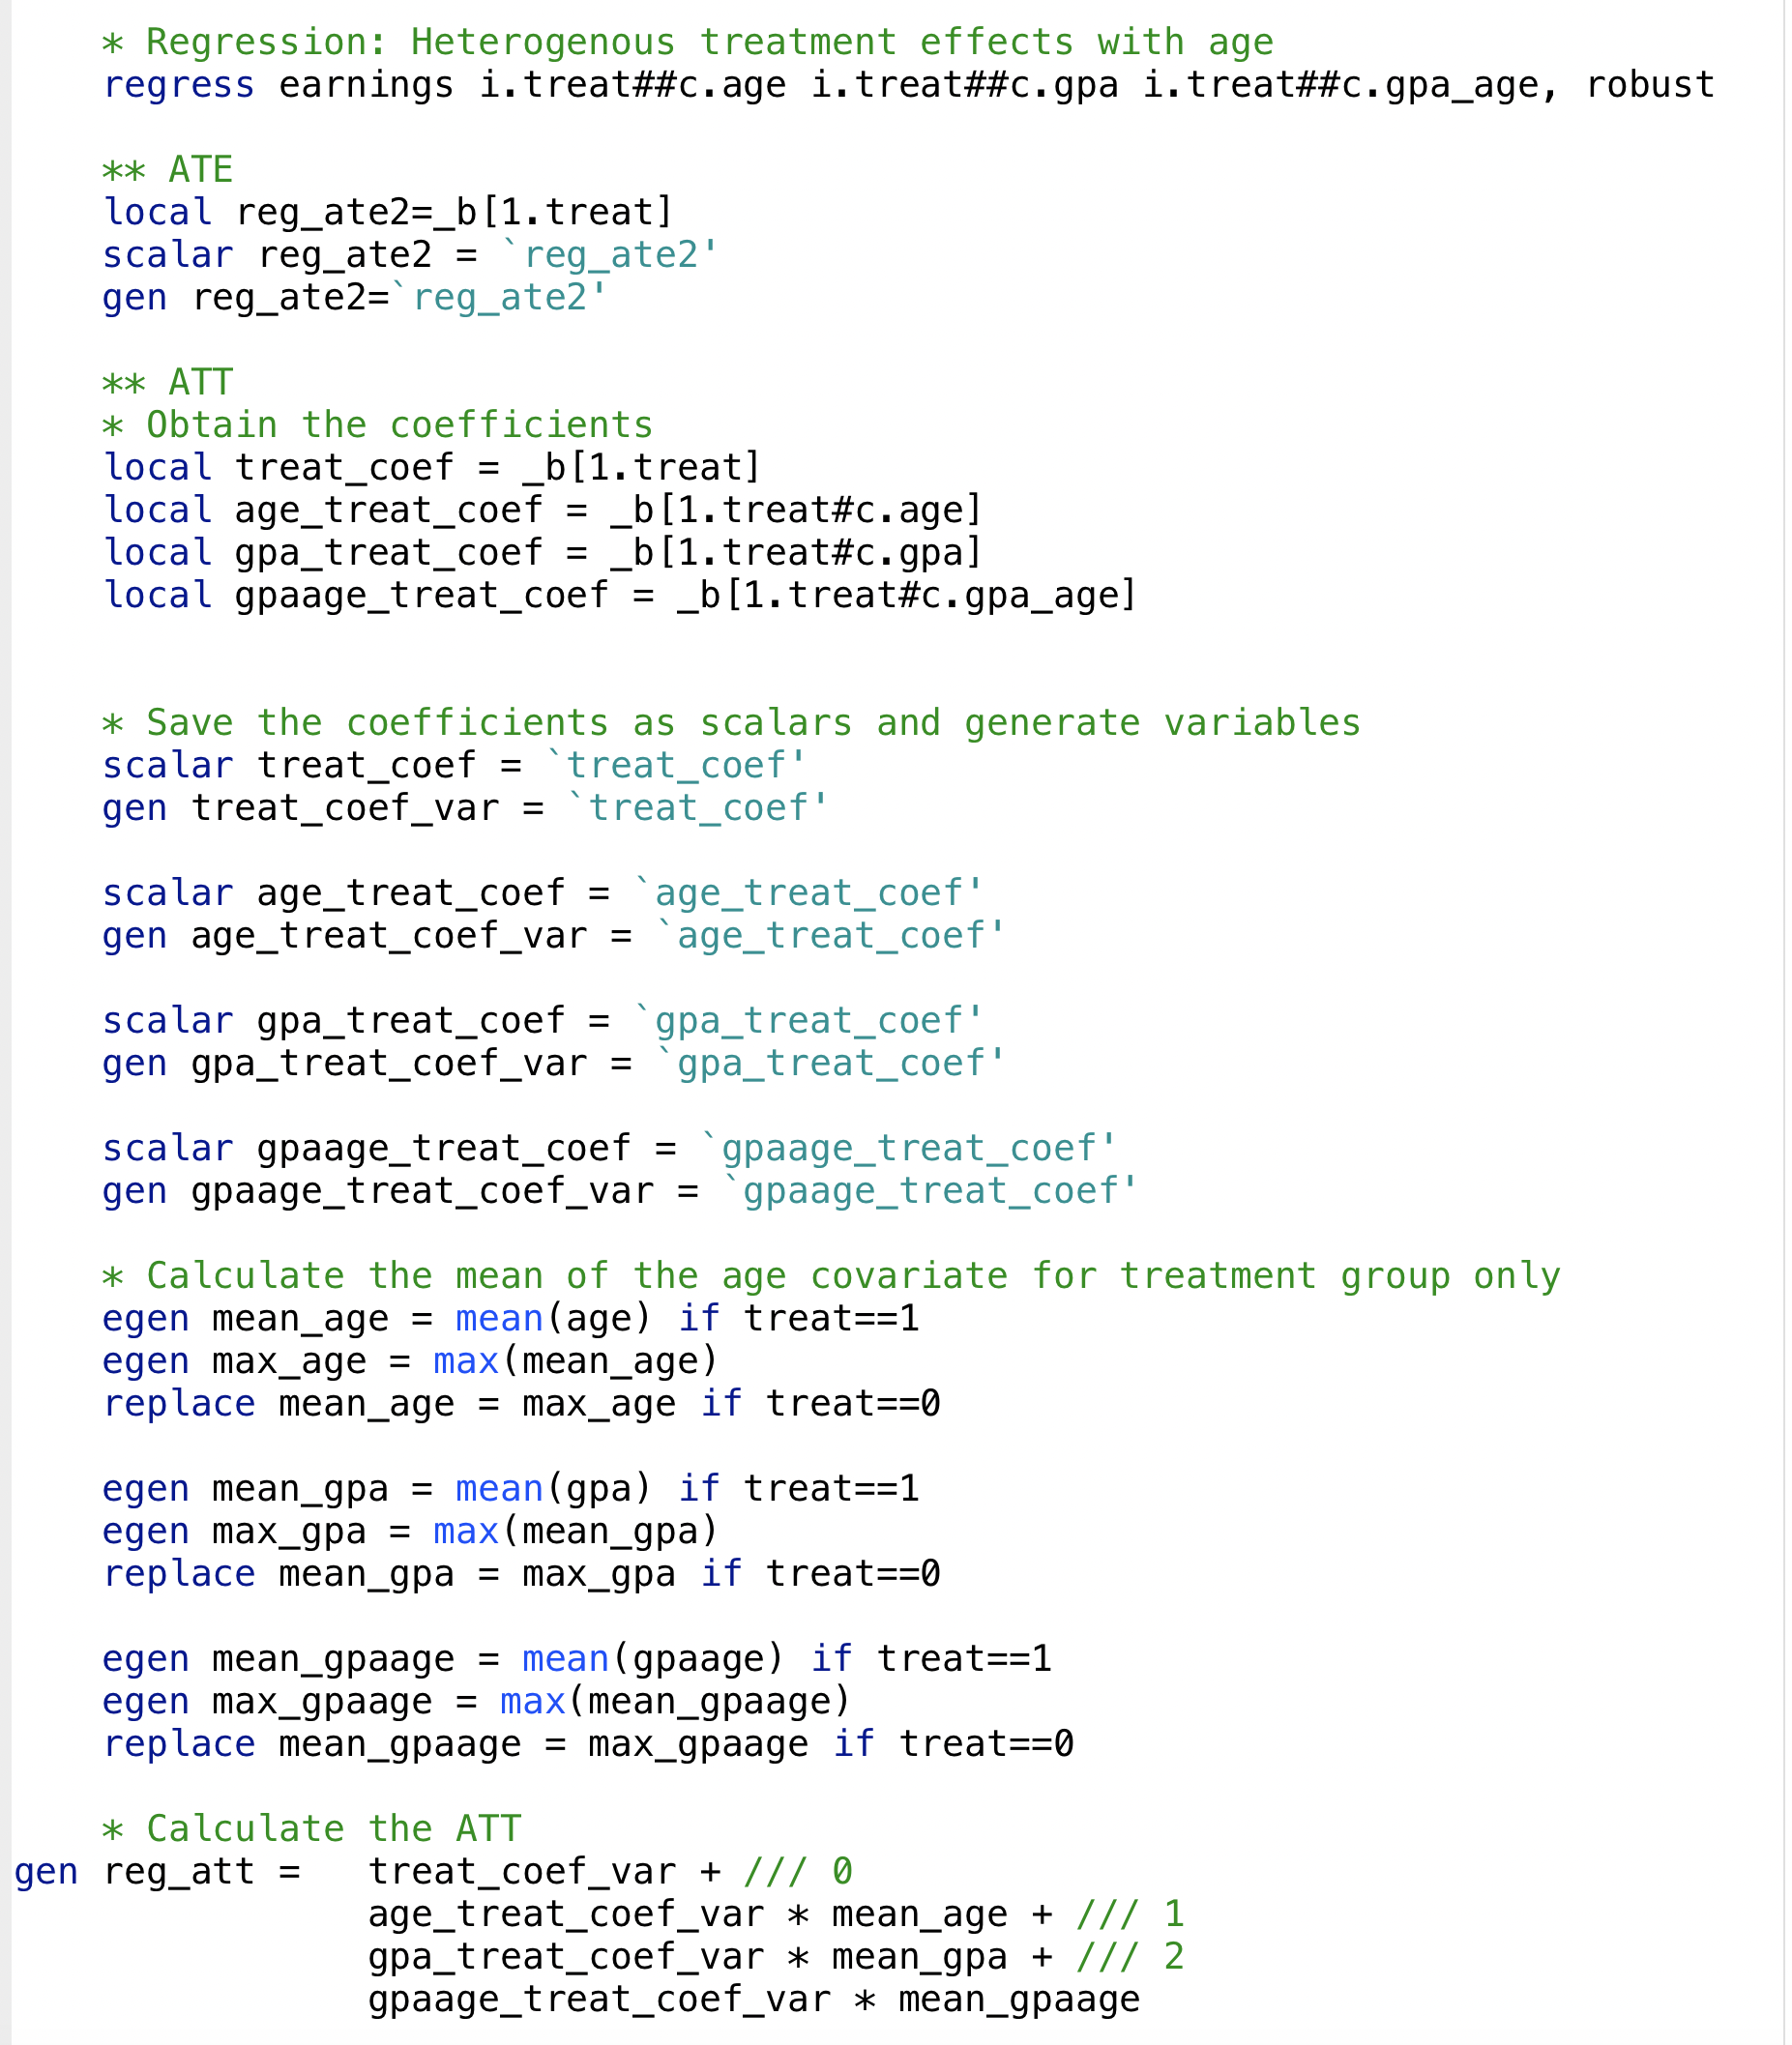
\includegraphics[scale=0.21]{./lecture_includes/nonlinear_ra}
\end{figure}

\end{frame}


\begin{frame}{Nonlinear DGP and Matching}

\begin{figure}[!t]\centering
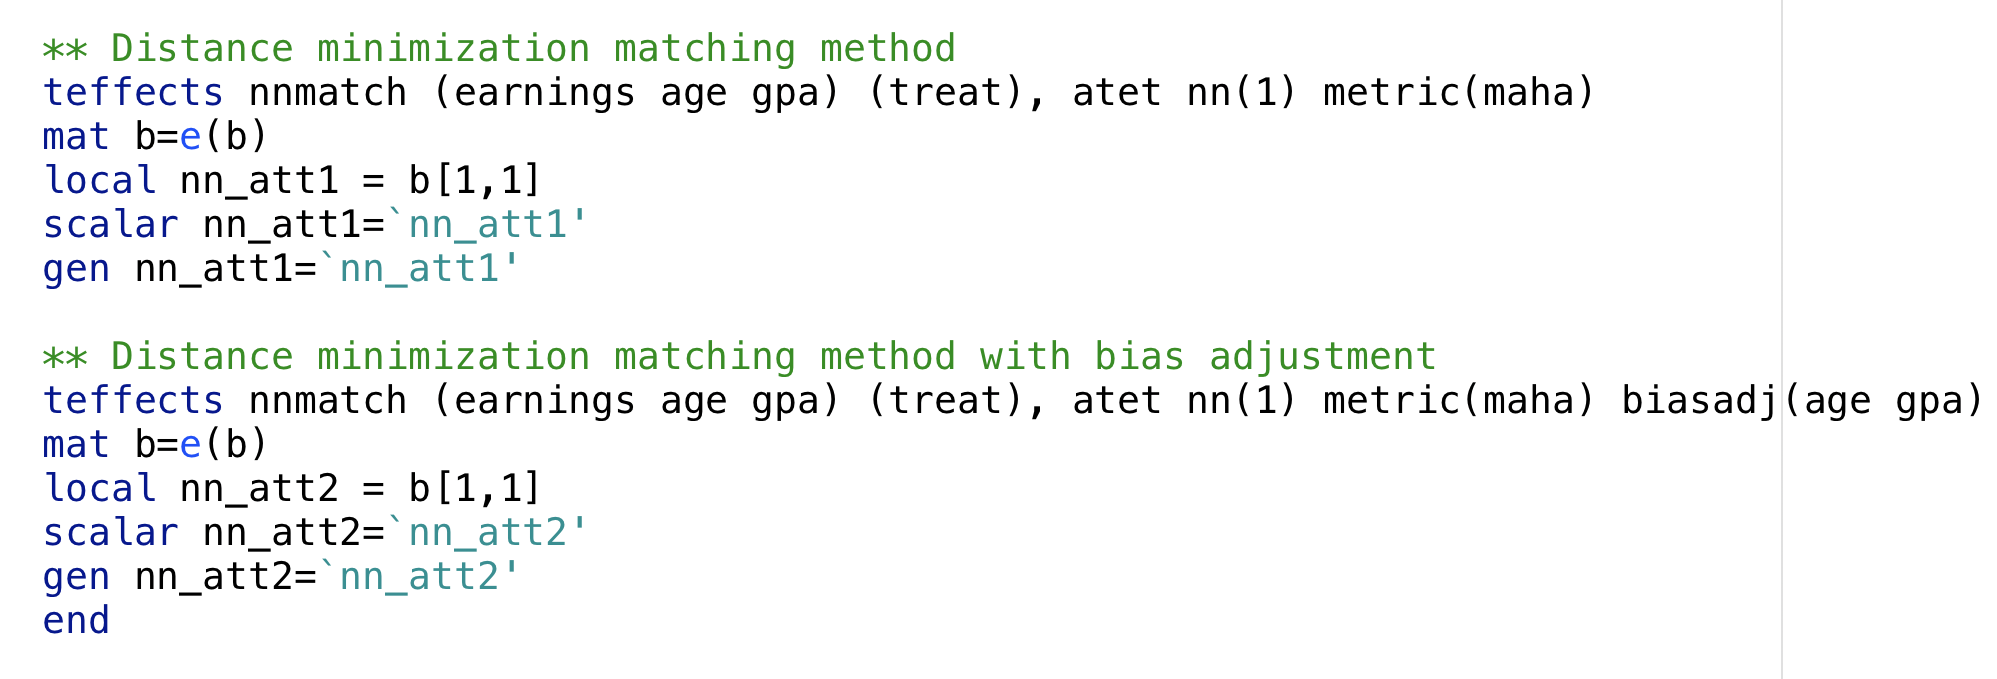
\includegraphics[scale=0.325]{./lecture_includes/nonlinear_matching}
\end{figure}

\end{frame}

\begin{frame}{Nonlinear DGP, OLS and Matching}

\begin{figure}[!t]\centering
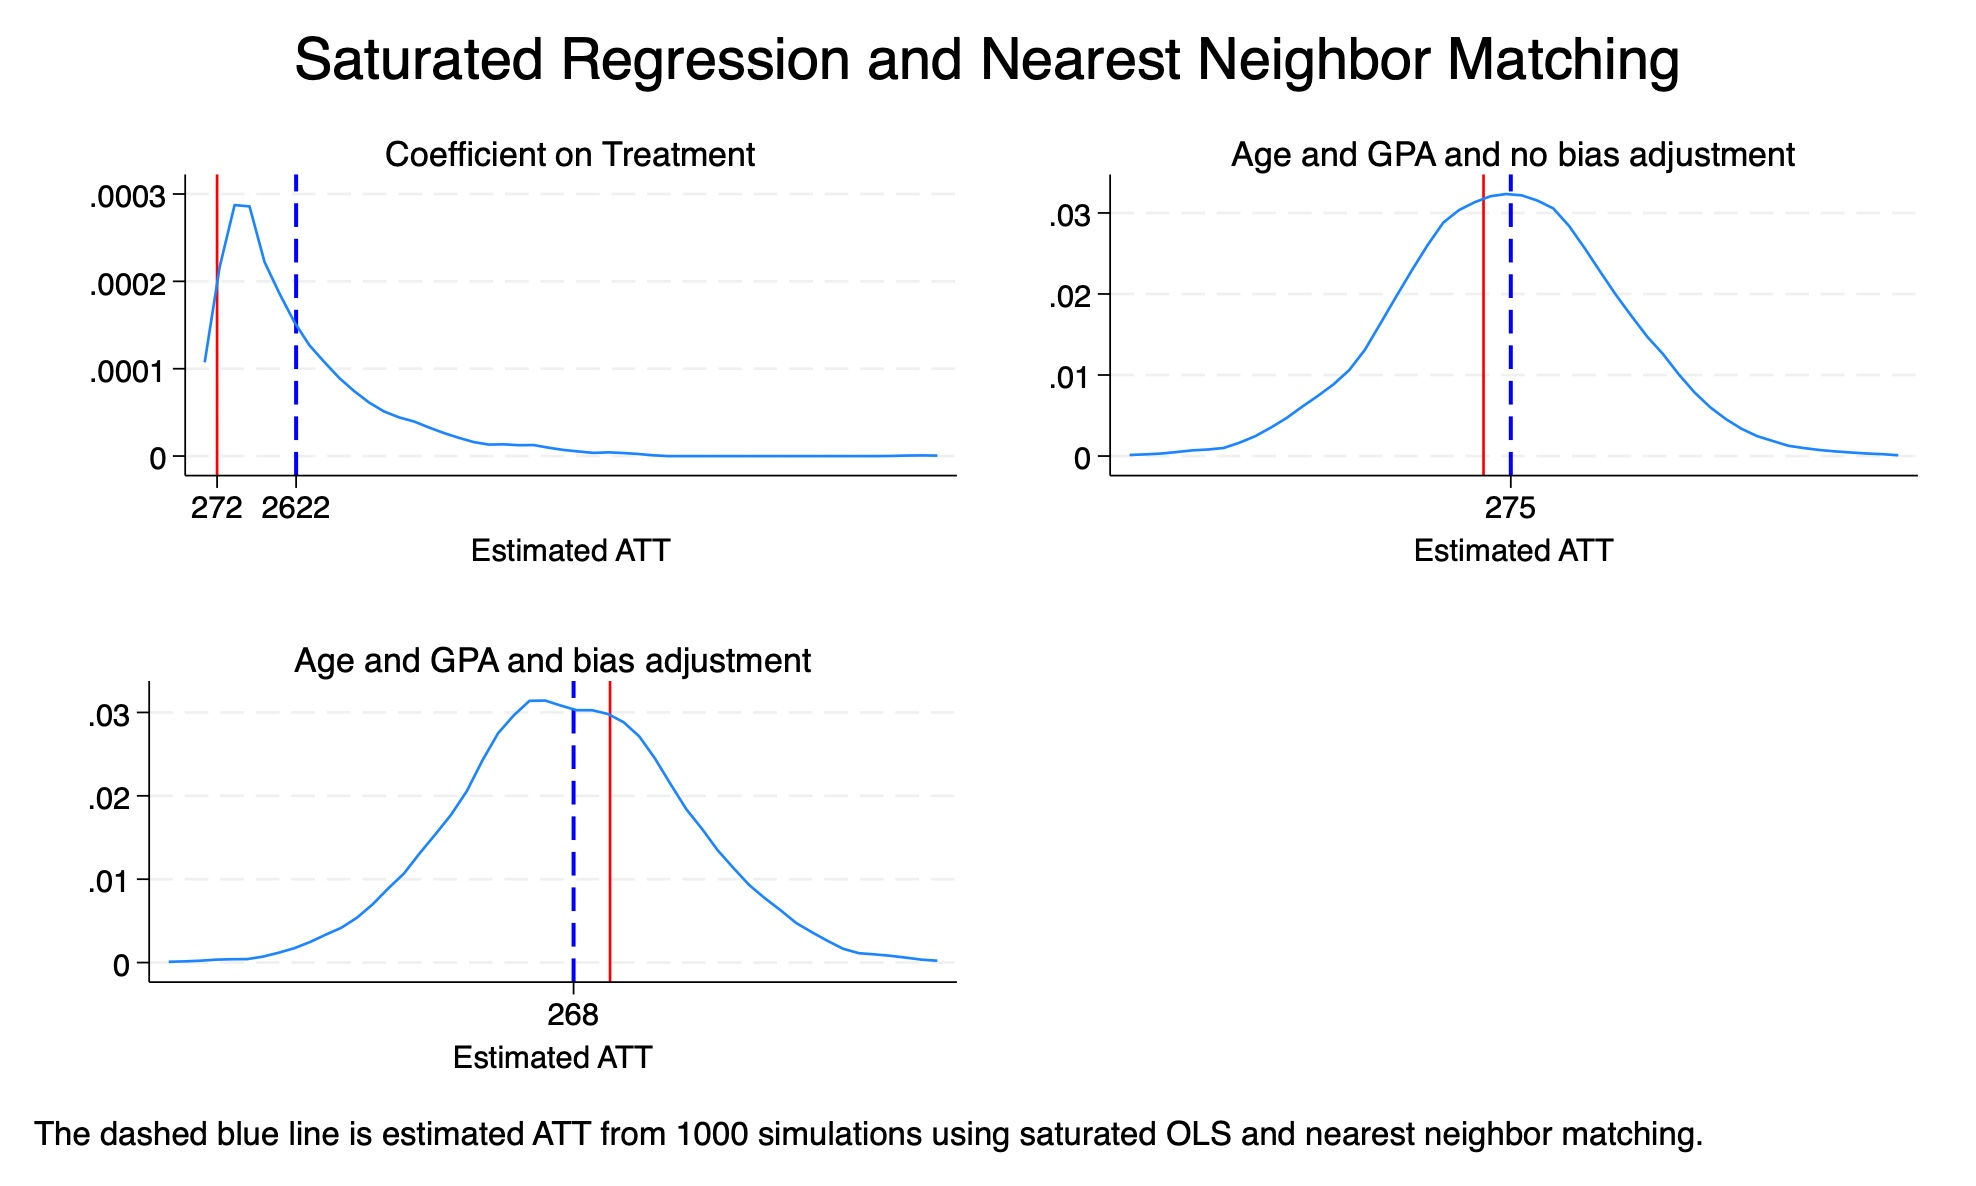
\includegraphics[scale=0.175]{./lecture_includes/nonlinear_att.jpg}
\end{figure}

\end{frame}





\begin{frame}\frametitle{Understanding the Standard OLS Model}
\begin{itemize}
  \item Tymon S{\l}oczy\'nski's 2022 Restat paper decomposes the following OLS model estimate of $\tau$ into weighted average of other parameters of interest
    \begin{equation}
      y = \alpha + \tau d + X \beta + u,
    \end{equation}
  \item Recall this is the model we found to have observed bias in earlier simulations due to the assumption of constant treatment effects (Imbens and Rubin 2015).
  \item But Tymon's paper addresses the interpretation of \(\tau\), the OLS estimand, when treatment effects are heterogeneous.
\end{itemize}
\end{frame}




\begin{frame}
\frametitle{Weights in Heterogeneous Treatment Effects}
\begin{itemize}
  \item With heterogeneous treatment effects, $\widehat{\tau}$ is both biased and pulled towards the smallest group's aggregate causal parameter(i.e., ATT vs ATU)
  \item In other words, the weight OLS places on the average effect for each group is inversely related to the group's size.
  \item As the number of treated units increases (as a fraction of the population), the weight on ATT \emph{decreases}
  \item This suggests OLS estimates based on this additive controls specification will be biased towards the smallest group's average treatment effect making it inappropriate when treatment effects vary across subjects
\end{itemize}
\end{frame}


\begin{frame}
\frametitle{A Pragmatic View of Heterogeneous Treatment Effects}
\begin{itemize}
  \item Tymon's paper provides a pragmatic perspective on the main result and derives corollaries suggesting diagnostic methods for when:
    \begin{enumerate}
      \item The treatment is binary.
      \item OLS is used.
      \item The researcher does not want to assume ATT = ATU.
    \end{enumerate}
  \item Diagnostics help detect when OLS weights deviate from what is needed for consistent estimation of ATE or ATT.
\end{itemize}
\end{frame}


\begin{frame}
\frametitle{Diagnostics for OLS with Heterogeneous Treatment Effects}
\begin{itemize}
  \item The diagnostics:
    \begin{itemize}
      \item Are bounded between 0 and 1 in absolute value.
      \item Reflect the proportion of bias from the difference between ATU and ATT.
    \end{itemize}
  \item A diagnostic close to 0 implies OLS may be suitable, while a value far from 0 suggests the need for alternative methods.
\end{itemize}
\end{frame}


\begin{frame}
\frametitle{Simple Diagnostics for ATT and ATE}
\begin{itemize}
  \item Special case diagnostics provide simple rules-of-thumb:
    \begin{itemize}
      \item For ATT estimation: Diagnostic is equal to the proportion of treated units, \( P(d = 1) \).
      \item For ATE estimation: Diagnostic is \( 2 \times P(d = 1) - 1 \), or twice the deviation from 50\%.
    \end{itemize}
  \item OLS approximates ATE well if the size of treated and untreated groups is similar.
  \item For ATT, a small proportion of treated units is necessary.
\end{itemize}
\end{frame}






\begin{frame}
\frametitle{Main Result: Algebra of OLS and Descriptive Estimands}
\begin{itemize}
    \item Focuses on the algebra of OLS and descriptive estimands.
    \item Potential outcomes and conditions for causal interpretation discussed in Section IIC.
    \item Main result does not require causal interpretation assumptions.
\end{itemize}
\end{frame}

\begin{frame}{Linear projection}

\begin{itemize}
\item Linear projection is a concept from the theory of linear regression describing the expected value of the dependent variable as a linear function of independent variables 
\item It does not necessarily incorporate randomness or an error term and so should be considered distinct from the ``data generating process'' which does
\item It posits a relationship that says, "If we knew the true parameters, this is how we would expect Y to change, on average, with changes in X and D"
\end{itemize}

\end{frame}


\begin{frame}
\frametitle{Linear Projection}
\begin{itemize}
    \item Let \( L(\cdot | \cdot) \) denote the linear projection.
    \item Interested in the interpretation of \( \tau \) in the linear projection of \( y \) on \( d \) and \( X \):
    \[ L(y | 1, d, X) = \alpha + \tau d + X\beta \quad \text{(2)} \]
    \item This projection is distinct from the structural conditional mean.
\end{itemize}
\end{frame}

\begin{frame}
\frametitle{Probability of Treatment and Propensity Score}
\begin{itemize}
    \item The unconditional probability of treatment:
    \[ \rho = P(d = 1) \quad \text{(3)} \]
    \item Propensity score from the linear probability model:
    \[ p(X) = L(d | 1, X) = \alpha_p + X\beta_p \quad \text{(4)} \]
    \item \( p(X) \) is the best linear approximation to the true propensity score.
    \item Equations (2) and (4) provide the specification.
\end{itemize}
\end{frame}

\begin{frame}
\frametitle{Flexibility of the Linear Projection}
\begin{itemize}
    \item Equation (2) can be seen as partially linear, including powers and cross-products of control variables.
    \item The propensity score approximation can be made very accurate.
\end{itemize}
\end{frame}

\begin{frame}
\frametitle{Linear Projections with Propensity Score}
\begin{itemize}
    \item Separate linear projections of \( y \) on \( p(X) \) for \( d = 1 \) and \( d = 0 \):
    \[ L[y | 1, p(X), d = 1] = \alpha_1 + \gamma_1 \times p(X) \quad \text{(5)} \]
    \[ L[y | 1, p(X), d = 0] = \alpha_0 + \gamma_0 \times p(X) \quad \text{(6)} \]
    \item Definitions are based on the variability of the propensity score within treatment groups.
\end{itemize}
\end{frame}

\begin{frame}
\frametitle{Assumptions for Linear Projections}
\begin{itemize}
    \item Assumption 1: Existence and uniqueness of linear projections in (2) and (4).
    \item Assumption 2: Existence and uniqueness of linear projections in (5) and (6).
    \item These assumptions guarantee the linear projections are well-defined and unique.
    \item Both of these assumptions (fn. 3) are generally innocuous although the second one rules out a small number of interesting applications like regression adjustments in completely randomized experiments -- but in these cases OLS will estimate the ATE consistently (Imbens and Rubin 2015)
\end{itemize}
\end{frame}

\begin{frame}
\frametitle{Defining Average Partial Linear Effects}
\begin{itemize}
    \item The average partial linear effect of \( d \):
    \[ \tau_{\text{APLE}} = (\alpha_1 - \alpha_0) + (\gamma_1 - \gamma_0) \times E[p(X)] \quad \text{(7)} \]
    \item The average partial linear effect of \( d \) on group \( j \) (where \( j = 0, 1 \)):
    \[ \tau_{\text{APLE}, j} = (\alpha_1 - \alpha_0) + (\gamma_1 - \gamma_0) \times E[p(X) | d = j] \quad \text{(8)} \]
    \item These estimands are well-defined under Assumptions 1 and 2.
\end{itemize}
\end{frame}

\begin{frame}
\frametitle{Causal Interpretation and Theorem 1}
\begin{itemize}
    \item Causal interpretation requires additional assumptions beyond 1 and 2.
    \item Theorem 1 is more general, relying only on Assumptions 1 and 2.
    \item It applies to the algebraic properties of OLS estimators.
\end{itemize}
\end{frame}


\begin{frame}
\frametitle{Weighted Average Interpretation of OLS (Theorem 1)}

Under assumptions (1) and (2)

$$\tau = \omega_1 \times \tau_{APLE,1} + \omega_0 \times \tau_{APLE,0}$$
 
 where the weights are equal to:
 
\begin{align*}
\omega_1 &= \frac{(1-\rho) \times V[p(X)|d=0]}{\rho \times V[p(X)|d=1] + (1-\rho) \times V[p(X)|d=0]} \\
\text{and} \quad \omega_0 &= 1 - \omega_1
\end{align*}

\end{frame}



\begin{frame}
\frametitle{Theorem 1: Interpretation of the OLS Estimand}
\begin{itemize}
    \item The OLS estimand \( \tau \) is a convex combination of \( \tau_{\text{APLE},1} \) and \( \tau_{\text{APLE},0} \).
    \item Reflects the weighted average outcome of a three-step procedure:
    \begin{enumerate}
        \item Obtain the propensity score \( p(X) \).
        \item Calculate \( \tau_{\text{APLE},1} \) and \( \tau_{\text{APLE},0} \) for \( d = 1 \) and \( d = 0 \) via linear projections.
        \item Compute the weighted average of \( \tau_{\text{APLE},1} \) and \( \tau_{\text{APLE},0} \).
    \end{enumerate}
\end{itemize}
\end{frame}


\begin{frame}
\frametitle{Weighting in the Estimation of \( \tau \)}
\begin{itemize}
    \item The weight on \( \tau_{\text{APLE},1} \), \( \omega_1 \), decreases with \( V[p(X) | d = 1] \) and the probability of treatment \( \rho \).
    \item Conversely, the weight on \( \tau_{\text{APLE},0} \), \( \omega_0 \), increases with \( V[p(X) | d = 1] \) and \( \rho \).
    \item The weighting scheme implies that larger groups receive less weight on their respective \( \tau_{\text{APLE},j} \).
\end{itemize}
\end{frame}


\begin{frame}{Assumptions for an Illustrative Example}
    The following graph shows how the weight on \( \tau_{\text{APLE},1} \) decreases as the variance of the propensity score among the treated increases using the following simplifications for illustrative purposes:
    \begin{itemize}
        \item The variance among the non-treated \( V[p(X) | d = 0] \) is constant at 0.1.
        \item The probability of treatment \( \rho \) is 0.5, meaning that half of the population is treated.
        \item The variance among the treated \( V[p(X) | d = 1] \) varies from 0.1 to 0.9 for the purpose of the illustration.
    \end{itemize}
\end{frame}


\begin{frame}{Weight on \( \tau_{\text{APLE},1} \) with Varying Variance among Treated}
    \begin{figure}
        \centering
        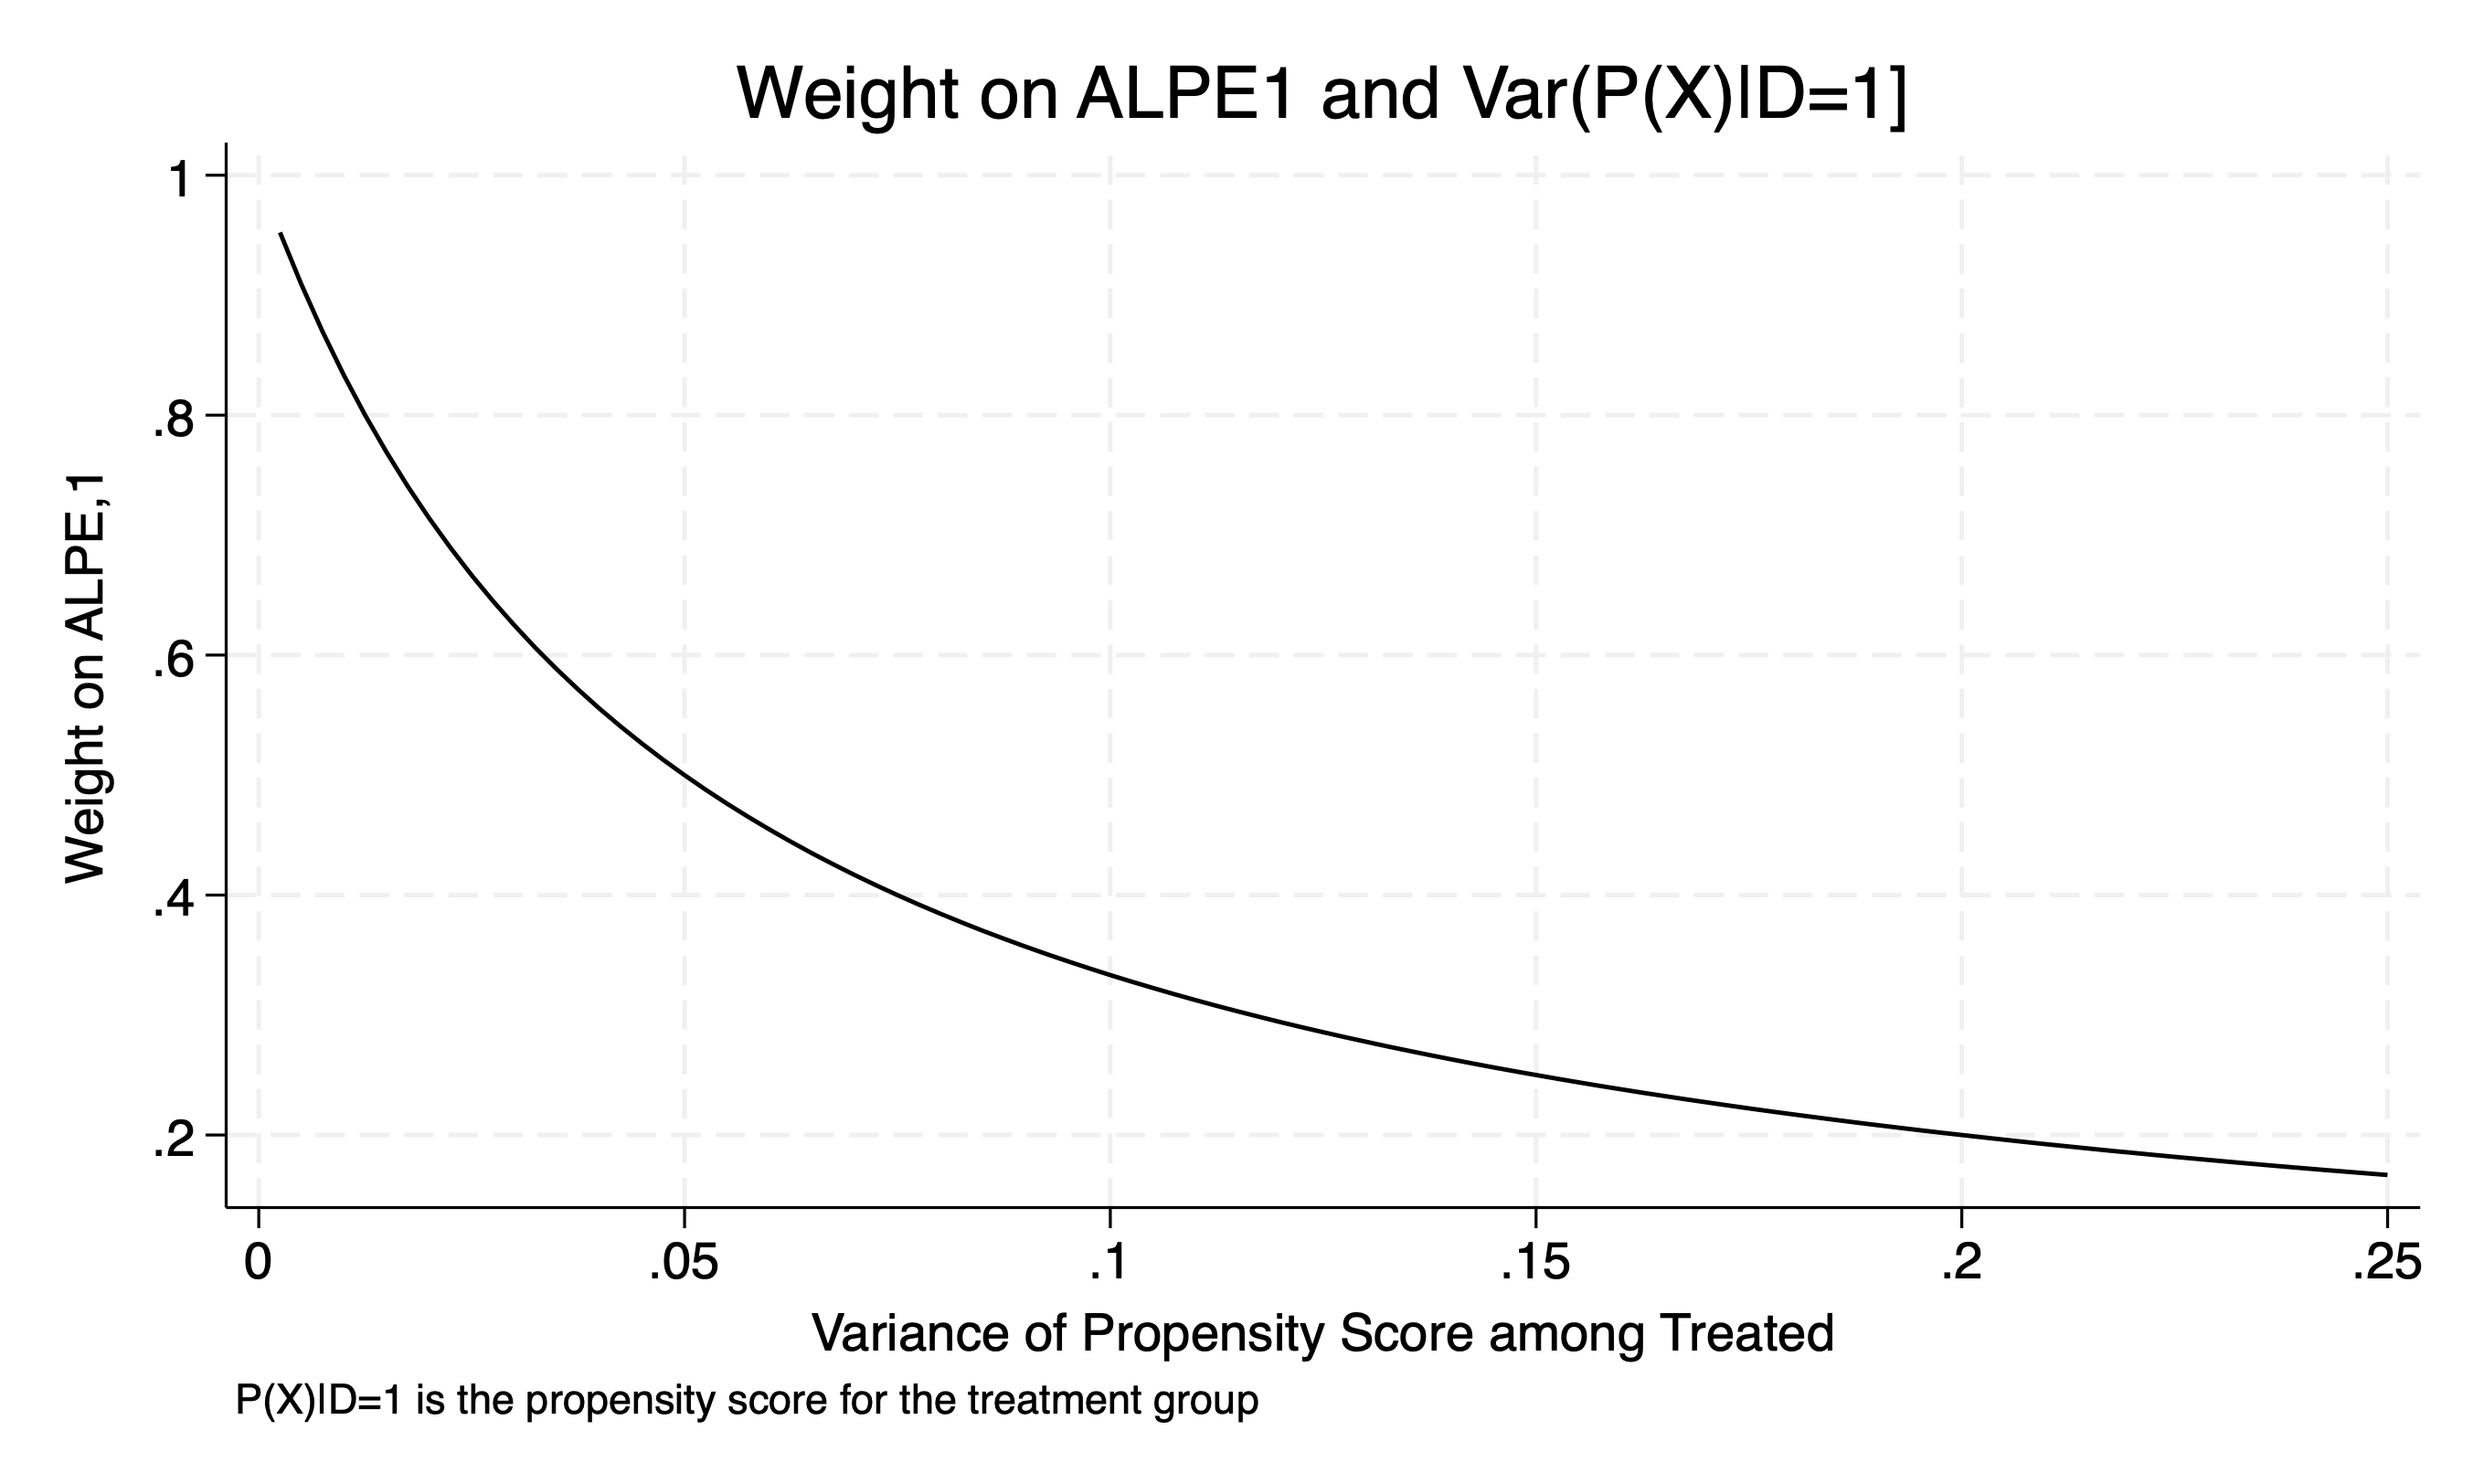
\includegraphics[width=0.8\textwidth]{./lecture_includes/tymon_variance_weight.png}
        \caption{The relationship between the weight \( \omega_1 \) on \( \tau_{\text{APLE},1} \) and the variance of the propensity score among the treated \( V[p(X) | d = 1] \). As the variance among the treated increases, the weight on \( \tau_{\text{APLE},1} \) decreases.}
    \end{figure}
\end{frame}

\begin{frame}{Factors Causing the Variance of the Propensity Score to Rise}


\textbf{Understanding Variance:}
\begin{itemize}
  \item The variance is not simply \( p(1-p) \) but the spread of the estimated propensity scores \( p(X) \) within the treatment group.
  \item It reflects the degree to which the likelihood of treatment (given covariates) varies among those actually treated.
\end{itemize}
\end{frame}




\begin{frame}{Factors Causing the Variance of the Propensity Score to Rise}
\textbf{The variance of the propensity score among the treated, \( V[p(X) | d = 1] \), can increase due to several factors:}

\begin{itemize}
  \item \alert{Heterogeneity in Covariates:} A diverse range of covariates within the treated group can lead to a wide array of propensity scores, increasing variance.
  \item \alert{Model Specification:} The choice of model and its ability to accurately capture the relationship between covariates and treatment affects variance. Mis-specification can inflate variance.
  \item \alert{Overlap with Control Group:} Significant overlap in propensity scores between treated and untreated groups can raise variance, reflecting less distinction based on covariates.
\end{itemize}

\end{frame}


\begin{frame}{Stata exercises}

We will now look at two simulations to help you understand both of these

\end{frame}



\begin{frame}
\frametitle{Intuition Behind the Weighting Scheme}
\begin{itemize}
    \item This counterintuitive result may be understood through the lens of finite sample properties.
    \item OLS places more weight on treatment effects that are more precisely estimated.
    \item Further intuition and alternative proof are provided in Online Appendix B2.
    \item The framework aligns with the insights from Angrist (1998) and Angrist and Pischke (2009) regarding the weighting of treatment effects in OLS.
\end{itemize}
\end{frame}

\begin{frame}{Causal Interpretation of OLS}
  Theorem 1 ("Weighted Average Interpretation of OLS") is general due to its reliance solely on the existence and uniqueness of linear projections; however, for a causal interpretation of OLS, we must introduce:
  \begin{itemize}
    \item Potential outcomes \( y(1) \) and \( y(0) \) instead of realized outcomes
    \item Defined causal parameters: ATE, ATT, and ATU
    \item Introduce assumptions that will ensure a causal interpretation of \( \tau \)
  \end{itemize}
\end{frame}

\begin{frame}{Assumption 3 for Causal Interpretation}
  \begin{block}{Unconfoundedness in Mean Potential Outcomes or "Ignorability in Means"}
    \begin{enumerate}
      \item \( E [y(1) | X, d] = E[y(1) | X] \)
      \item \( E[y(0) | X, d] = E[y(0) | X] \)
    \end{enumerate}
  \end{block}
  Assumptions 3 is our standard unconfoundedness assumption but limited to means (slightly weaker but it's all we need)
\end{frame}

\begin{frame}{Assumption 4 for Causal Interpretation}
  \begin{block}{Linearity in Potential Outcomes}
    Assumption 4 posits that the conditional expectations of potential outcomes are linear in the propensity score:
    \begin{enumerate}
      \item \( E[y(1) | X] = \alpha_1 + \gamma_1 \times p(X) \)
      \item \( E[y(0) | X] = \alpha_0 + \gamma_0 \times p(X) \)
    \end{enumerate}
  \end{block}
\end{frame}

\begin{frame}{Historical and Practical Context of Assumption 4}
  While not a common assumption, it is not necessarily strong due to:
  \begin{itemize}
    \item The flexibility in the specification of \( X \), which can include nonlinear terms.
    \item The automatic satisfaction of this assumption in saturated models.
  \end{itemize}

    The linearity assumption has historical roots and practical implications:
    \begin{itemize}
      \item Historically aligned with Rosenbaum and Rubin (1983).
      \item Assumed linearity of \( E[d | X] \) in several notable econometric works.
      \item It is restrictive but can be mitigated by model specification choices.
    \end{itemize}
\end{frame}


\begin{frame}{Corollary 1: Causal Interpretation of OLS}
  Under assumptions the first two linear projection related assumptions and these two new causal assumptions, then
  \[
    \tau = \omega_1 \times \tau_{\text{ATT}} + \omega_0 \times \tau_{\text{ATU}}
  \]
  
  In words, this states that under those four assumptions, the OLS weights from theorem 1 apply to the causal parameters we care about, the ATT and the ATU, and so therefore $\tau$ has a causal interpretation.  
  
  \bigskip
  
  But there's a catch: the greater the proportion of treated units, the smaller the OLS weight on the ATT, which is a problem given ATE = $\rho \times ATT + (1-\rho) ATU$
\end{frame}

\begin{frame}{Proving Corollary 1 with Assumptions 3 and 4}
  \begin{itemize}
    \item Assumption 3 (Unconfoundedness) allows us to estimate the ATE using realized outcomes, as the expected potential outcomes are equal to the observed outcomes conditional on covariates \( X \):
    \[ E[y(1) - y(0) | X] = E[y | X, d = 1] - E[y | X, d = 0] \]
    \item Assumption 4 specifies the functional form of the expected potential outcomes as linear in the propensity score:
    \[ E[y(1) | X] = \alpha_1 + \gamma_1 \times p(X), \quad E[y(0) | X] = \alpha_0 + \gamma_0 \times p(X) \]
    \item Together, they imply that the OLS estimand for the treated (\( \tau_{\text{ATT}} \)) and untreated (\( \tau_{\text{ATU}} \)) equates to the Average Partial Linear Effects (APLE):
    \[ \tau_{\text{ATT}} = \tau_{\text{APLE},1}, \quad \tau_{\text{ATU}} = \tau_{\text{APLE},0} \]
    \item This connects the causal treatment effects (ATT and ATU) directly to the estimated effects from the linear projections.
  \end{itemize}
\end{frame}


\begin{frame}{OLS Weights and Causal Parameters}
  \begin{itemize}
  \item Note earlier I said "there's a catch" -- the OLS weights are inversely related to the size of the treatment group shares
    \item The greater the proportion of treated units, the smaller the weight on \( \tau_{\text{ATT}} \) in the OLS estimand.
    \item The OLS approach is optimal for predicting actual outcomes, not necessarily for causal inference which aims at predicting counterfactuals.
  \end{itemize}
\end{frame}



\begin{frame}{Visualizing the problem one way}
    \begin{figure}
        \centering
        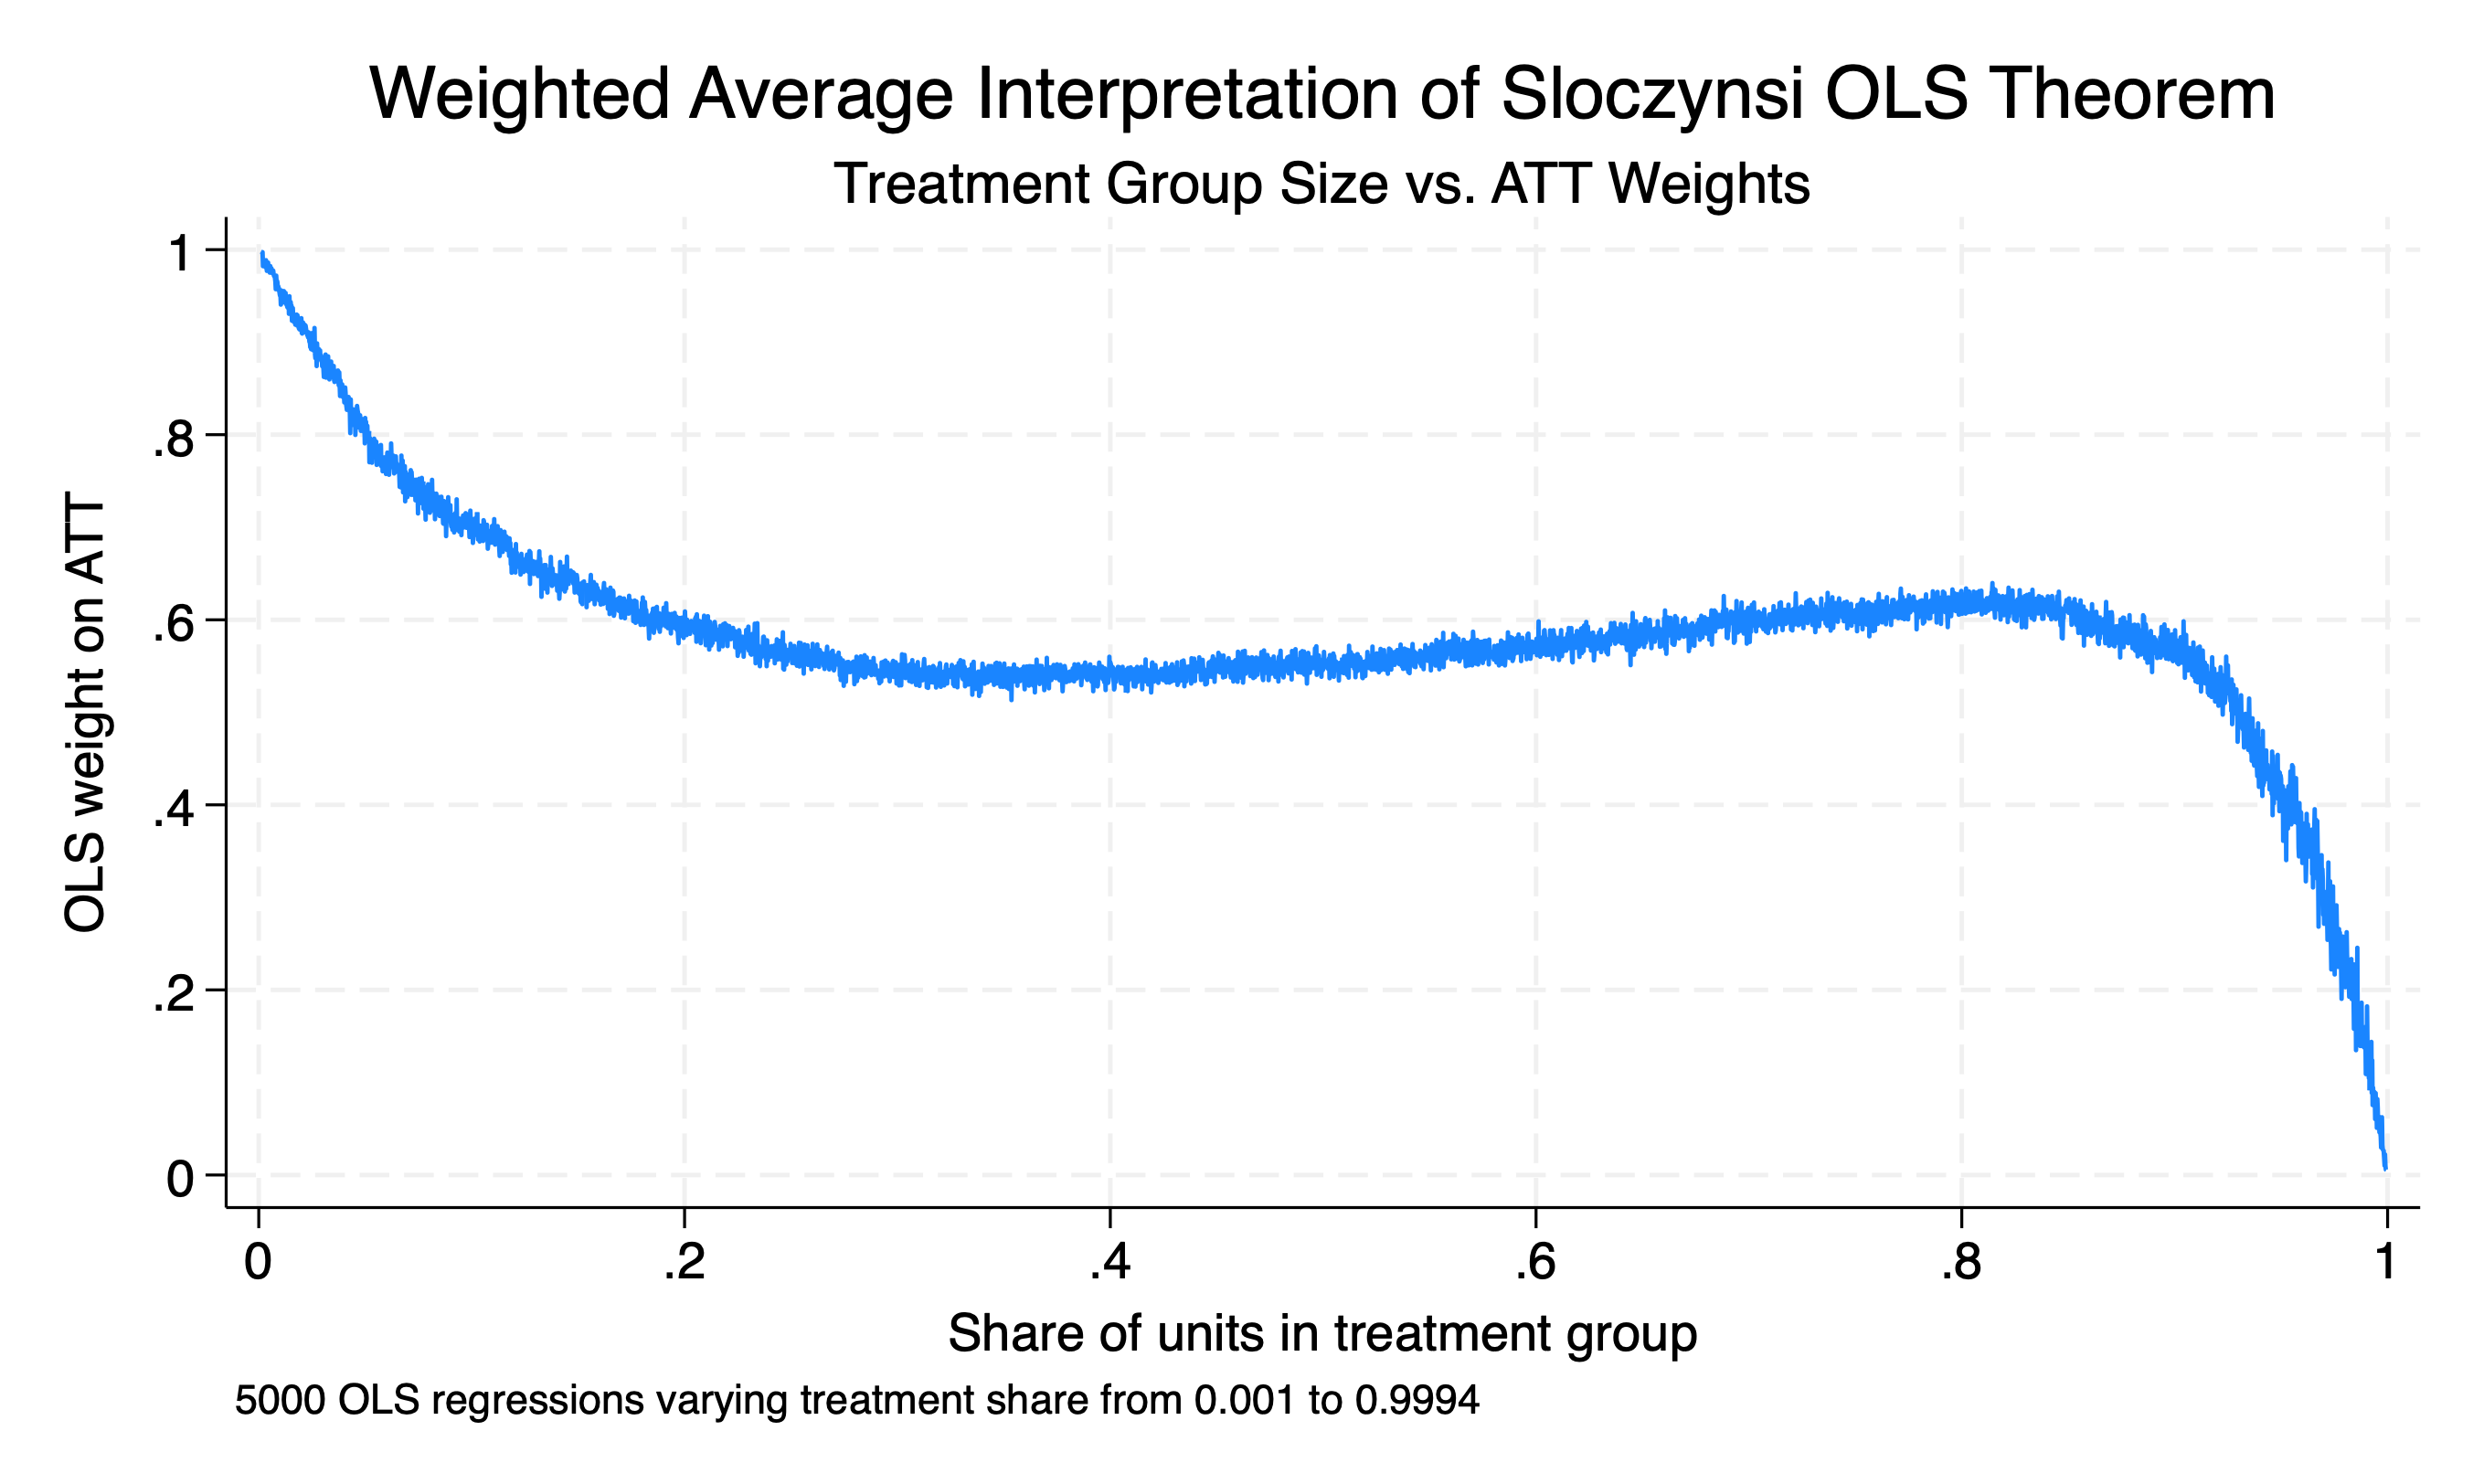
\includegraphics[width=0.8\textwidth]{./lecture_includes/tymon_weights_crossing}
        \caption{As more units are placed in treatment (blue line), the weight OLS places on the ATT.}
    \end{figure}
\end{frame}

\begin{frame}{Visualizing the problem another way}
    \begin{figure}
        \centering
        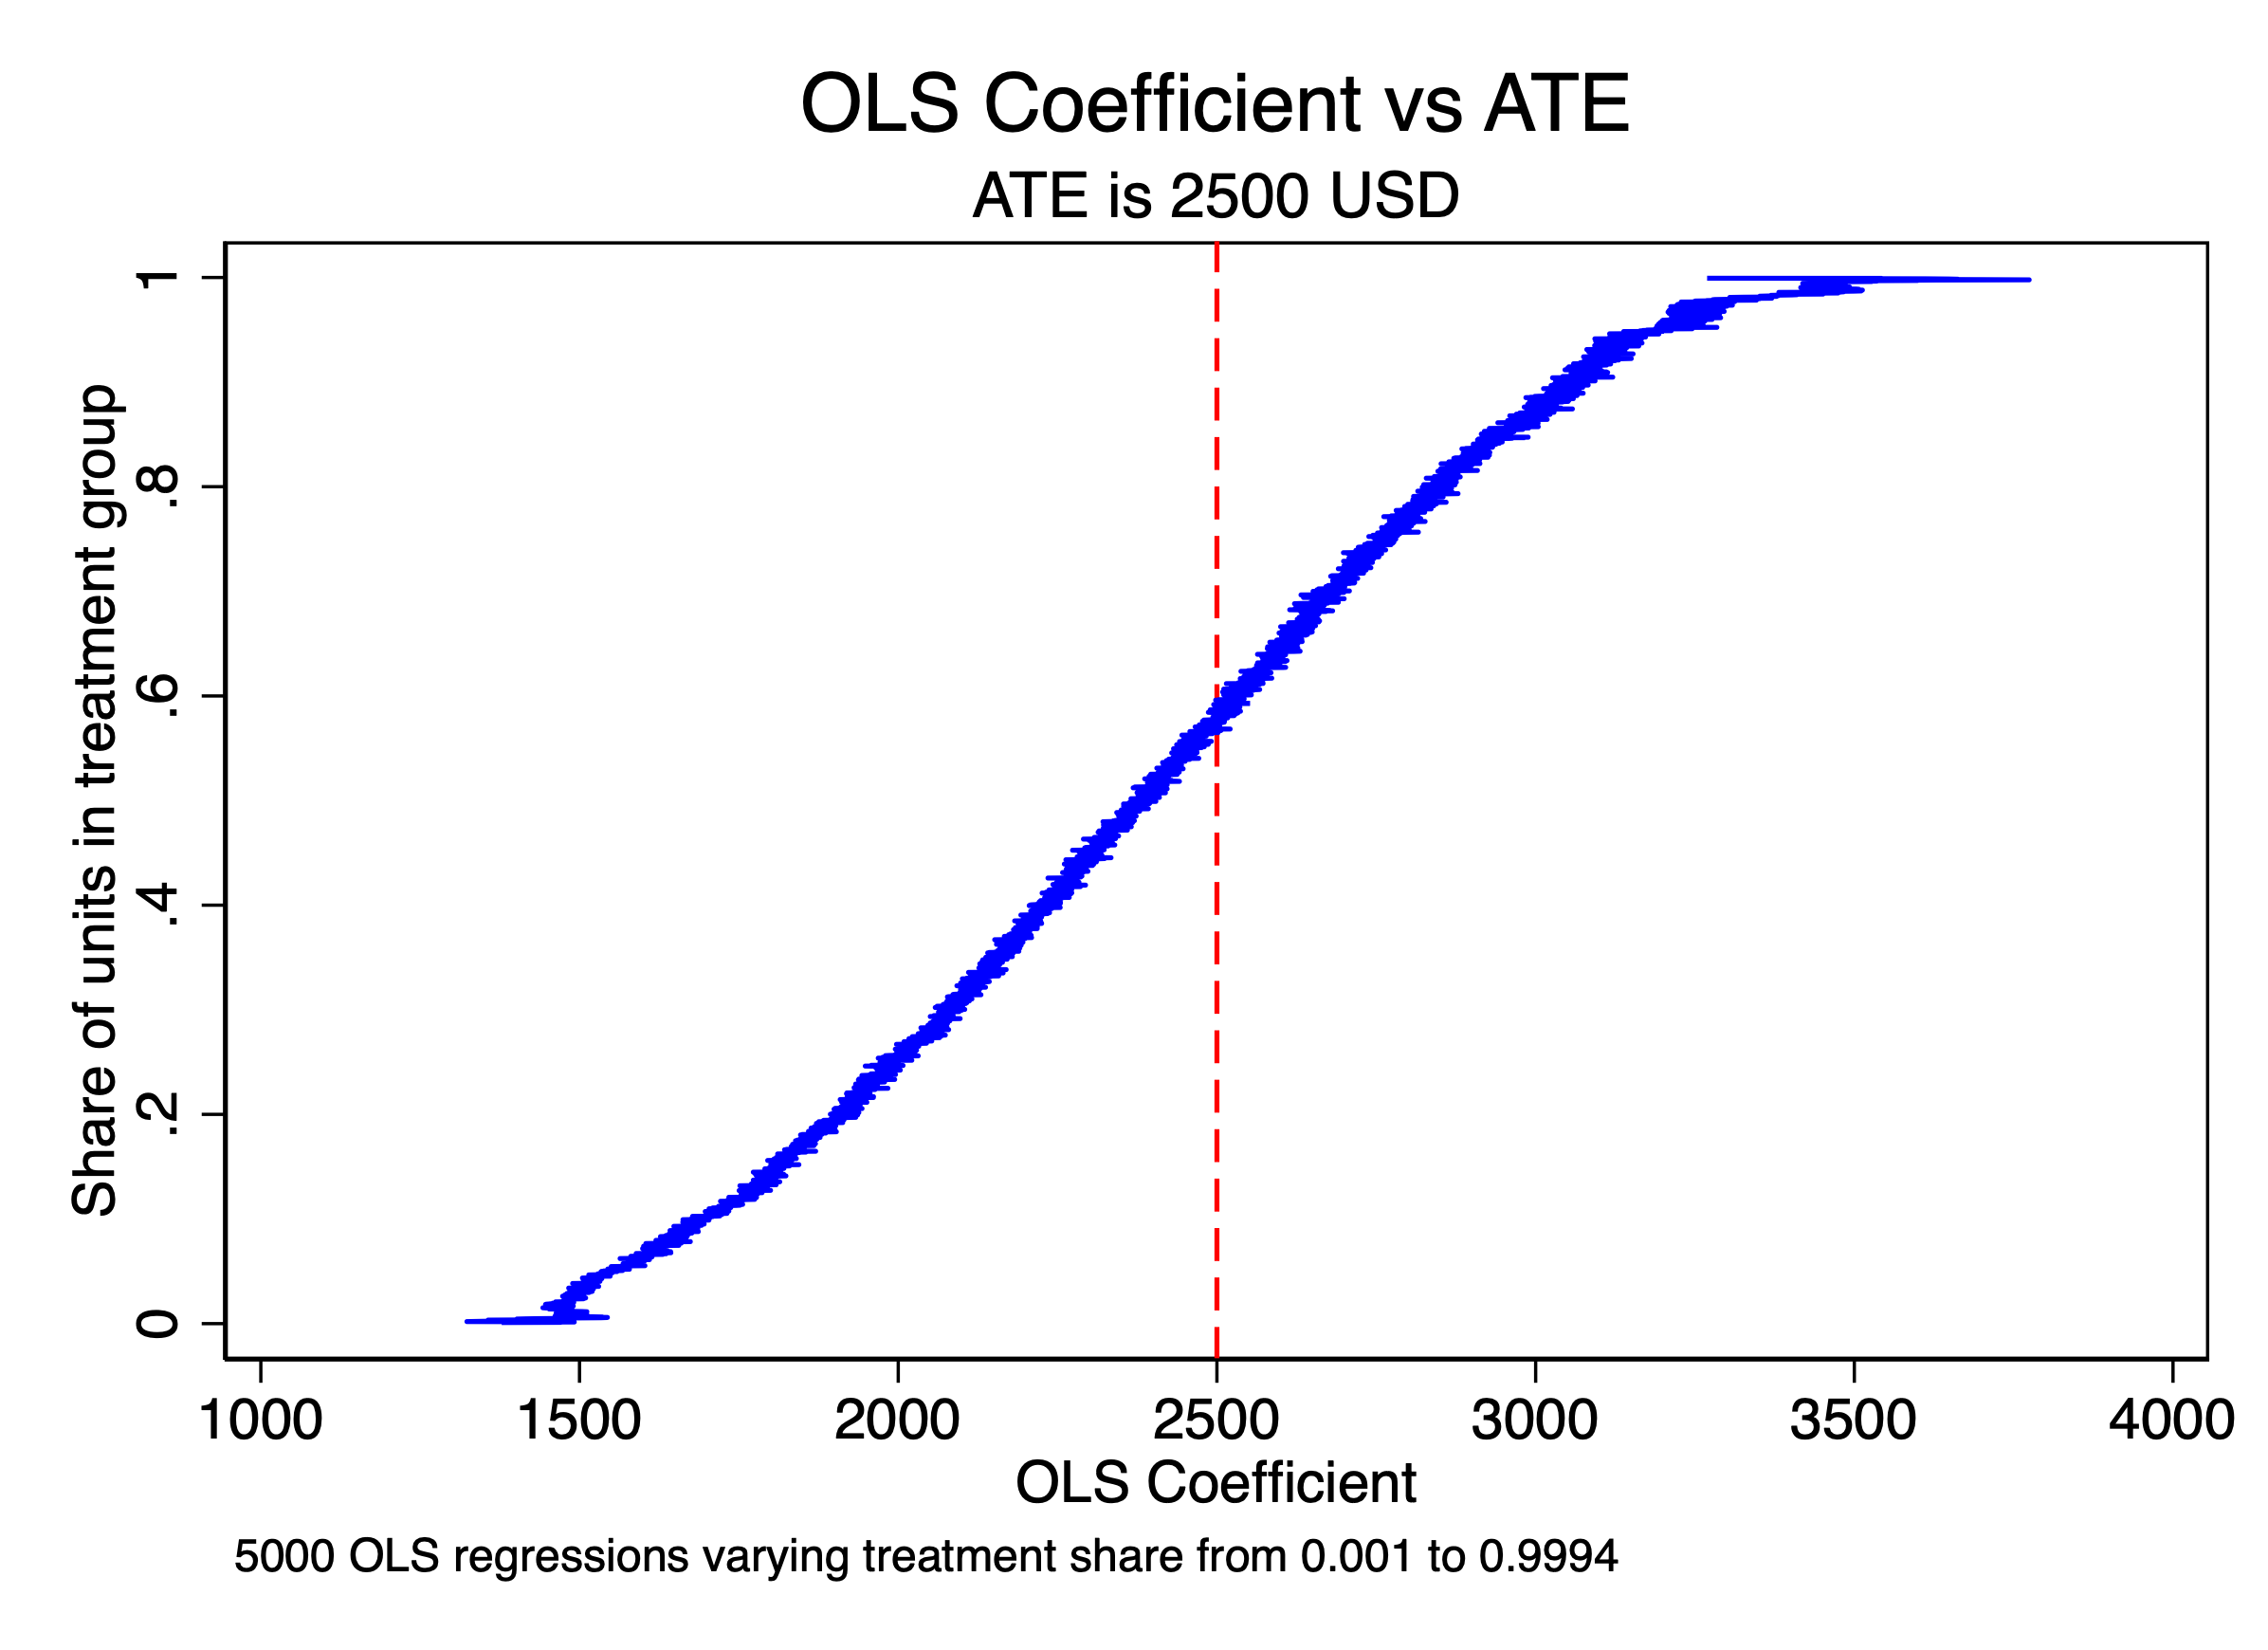
\includegraphics[width=0.8\textwidth]{./lecture_includes/ols_ate.png}
        \caption{As more units are placed in treatment (top right), OLS is weighted \emph{towards} the ATU (\$3,037) and when few are in the treatment (bottom left), it is weighted towards the ATT (\$1,962) }
    \end{figure}
\end{frame}



\begin{frame}{Predicting Outcomes vs. Predicting Counterfactuals}
  \begin{itemize}
    \item OLS prioritizes weights based on the size of the group when predicting actual outcomes.
    \item For causal inference (predicting counterfactuals), the emphasis should be on the coefficients predicting outcomes for the smaller group.
  \end{itemize}
\end{frame}

\begin{frame}{Adjustment for Predicting Counterfactuals}

\tiny
  \[
    \tau_{\text{ATE}} = [E(y|d=1) - E(y|d=0)] - [(1 - \rho)\beta_1 + \rho\beta_0] \times [E(X | d = 1) - E(X | d = 0)]
  \]
  \begin{itemize}
    \item OLS and ATE share structural similarities but differ in weight assignment.
    \item In ATE, larger groups receive smaller weights on their specific coefficients, opposite to OLS weighting.
  \end{itemize}
\end{frame}


\begin{frame}{Bias of coefficients}
    \begin{figure}
        \centering
        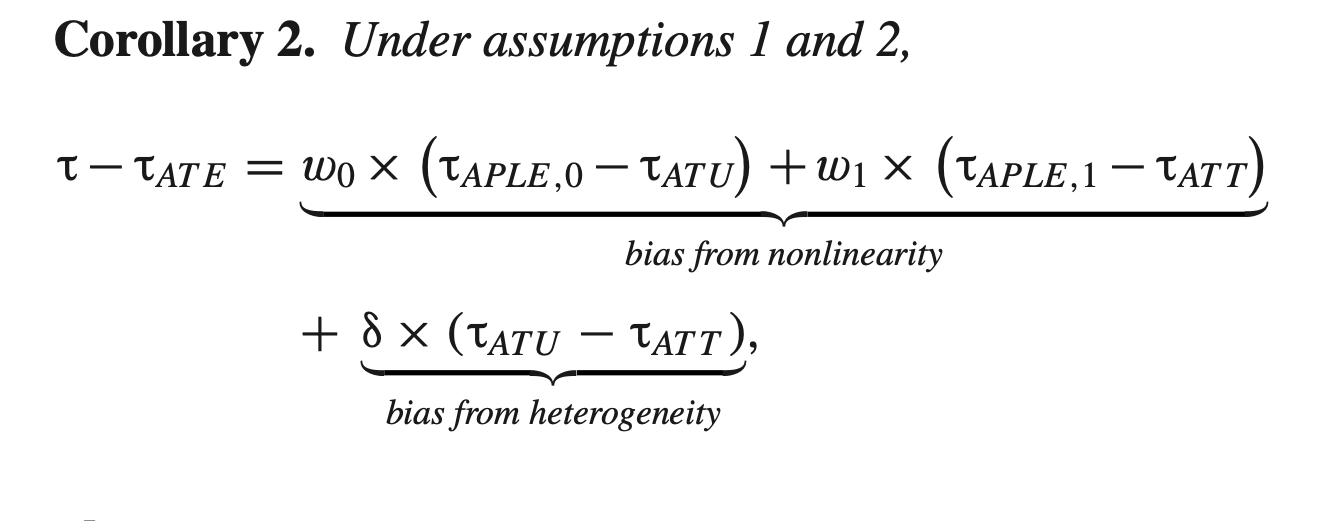
\includegraphics[width=0.8\textwidth]{./lecture_includes/ols_bias1.png}
    \end{figure}
\end{frame}


\begin{frame}{Bias of coefficients}
    \begin{figure}
        \centering
        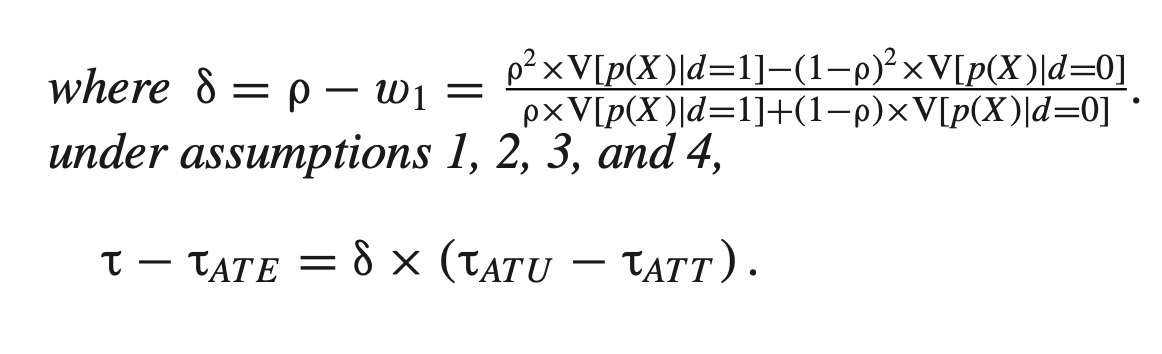
\includegraphics[width=0.8\textwidth]{./lecture_includes/ols_bias2.png}
    \end{figure}
\end{frame}

\begin{frame}{Bias of coefficients}
    \begin{figure}
        \centering
        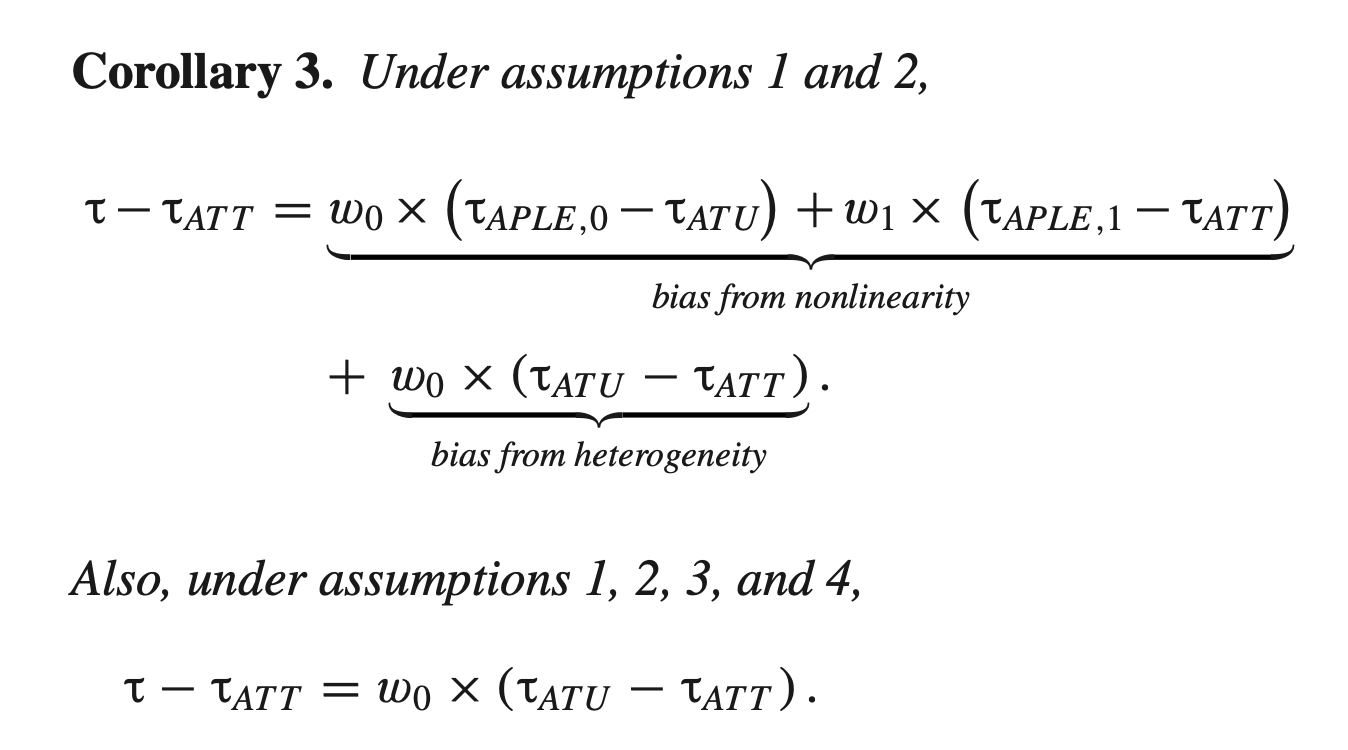
\includegraphics[width=0.8\textwidth]{./lecture_includes/ols_bias3.png}
    \end{figure}
\end{frame}


\begin{frame}
\frametitle{Prevalence of OLS Bias in Evaluating Labor Market Programs}
\begin{itemize}
  \item OLS may frequently show substantial bias for ATE and ATT in published studies
  \item In studies like Card, Kluve, and Weber (2018), with a mean treatment rate of 17.7\%, biases are common:
    \begin{itemize}
      \item The expected bias in OLS for ATE is 64.6\% of the ATU-ATT difference.
      \item For ATT, the expected OLS bias is 17.7\% of the ATU-ATT difference.
    \end{itemize}
  \item These findings indicate that biases in OLS estimates could often be significant.
    \begin{itemize}
      \item LaLonde's (1986) training program effects aligning with ATT.
      \item Aizer et al.'s (2016) cash transfer effects resembling ATU.
    \end{itemize}
  \item Implementation of results is available in R and Stata through the \texttt{hettreatreg} packages.
\end{itemize}
\end{frame}


\begin{frame}
\frametitle{Issues with OLS Weights Illustrated by the NSW Program}
\begin{itemize}
  \item NSW program provides a classic example of OLS weights problem.
  \item LaLonde (1986) and Angrist and Pischke (2009) assessments using the Dehejia and Wahba (2002) subsample (see Stata code together)
    \begin{itemize}
      \item OLS close to experimental benchmark but driven by a small treated sample.
      \item Economic disadvantage of treated vs. CPS comparison group suggests large ATT and ATU differences.
    \end{itemize}
  \item Treated sample's size (1.1\%) implies that OLS will be skewed towards the ATT 
\end{itemize}
\end{frame}


\begin{frame}{Tymon's replication of Angrist and Pischke}
    \begin{figure}
        \centering
        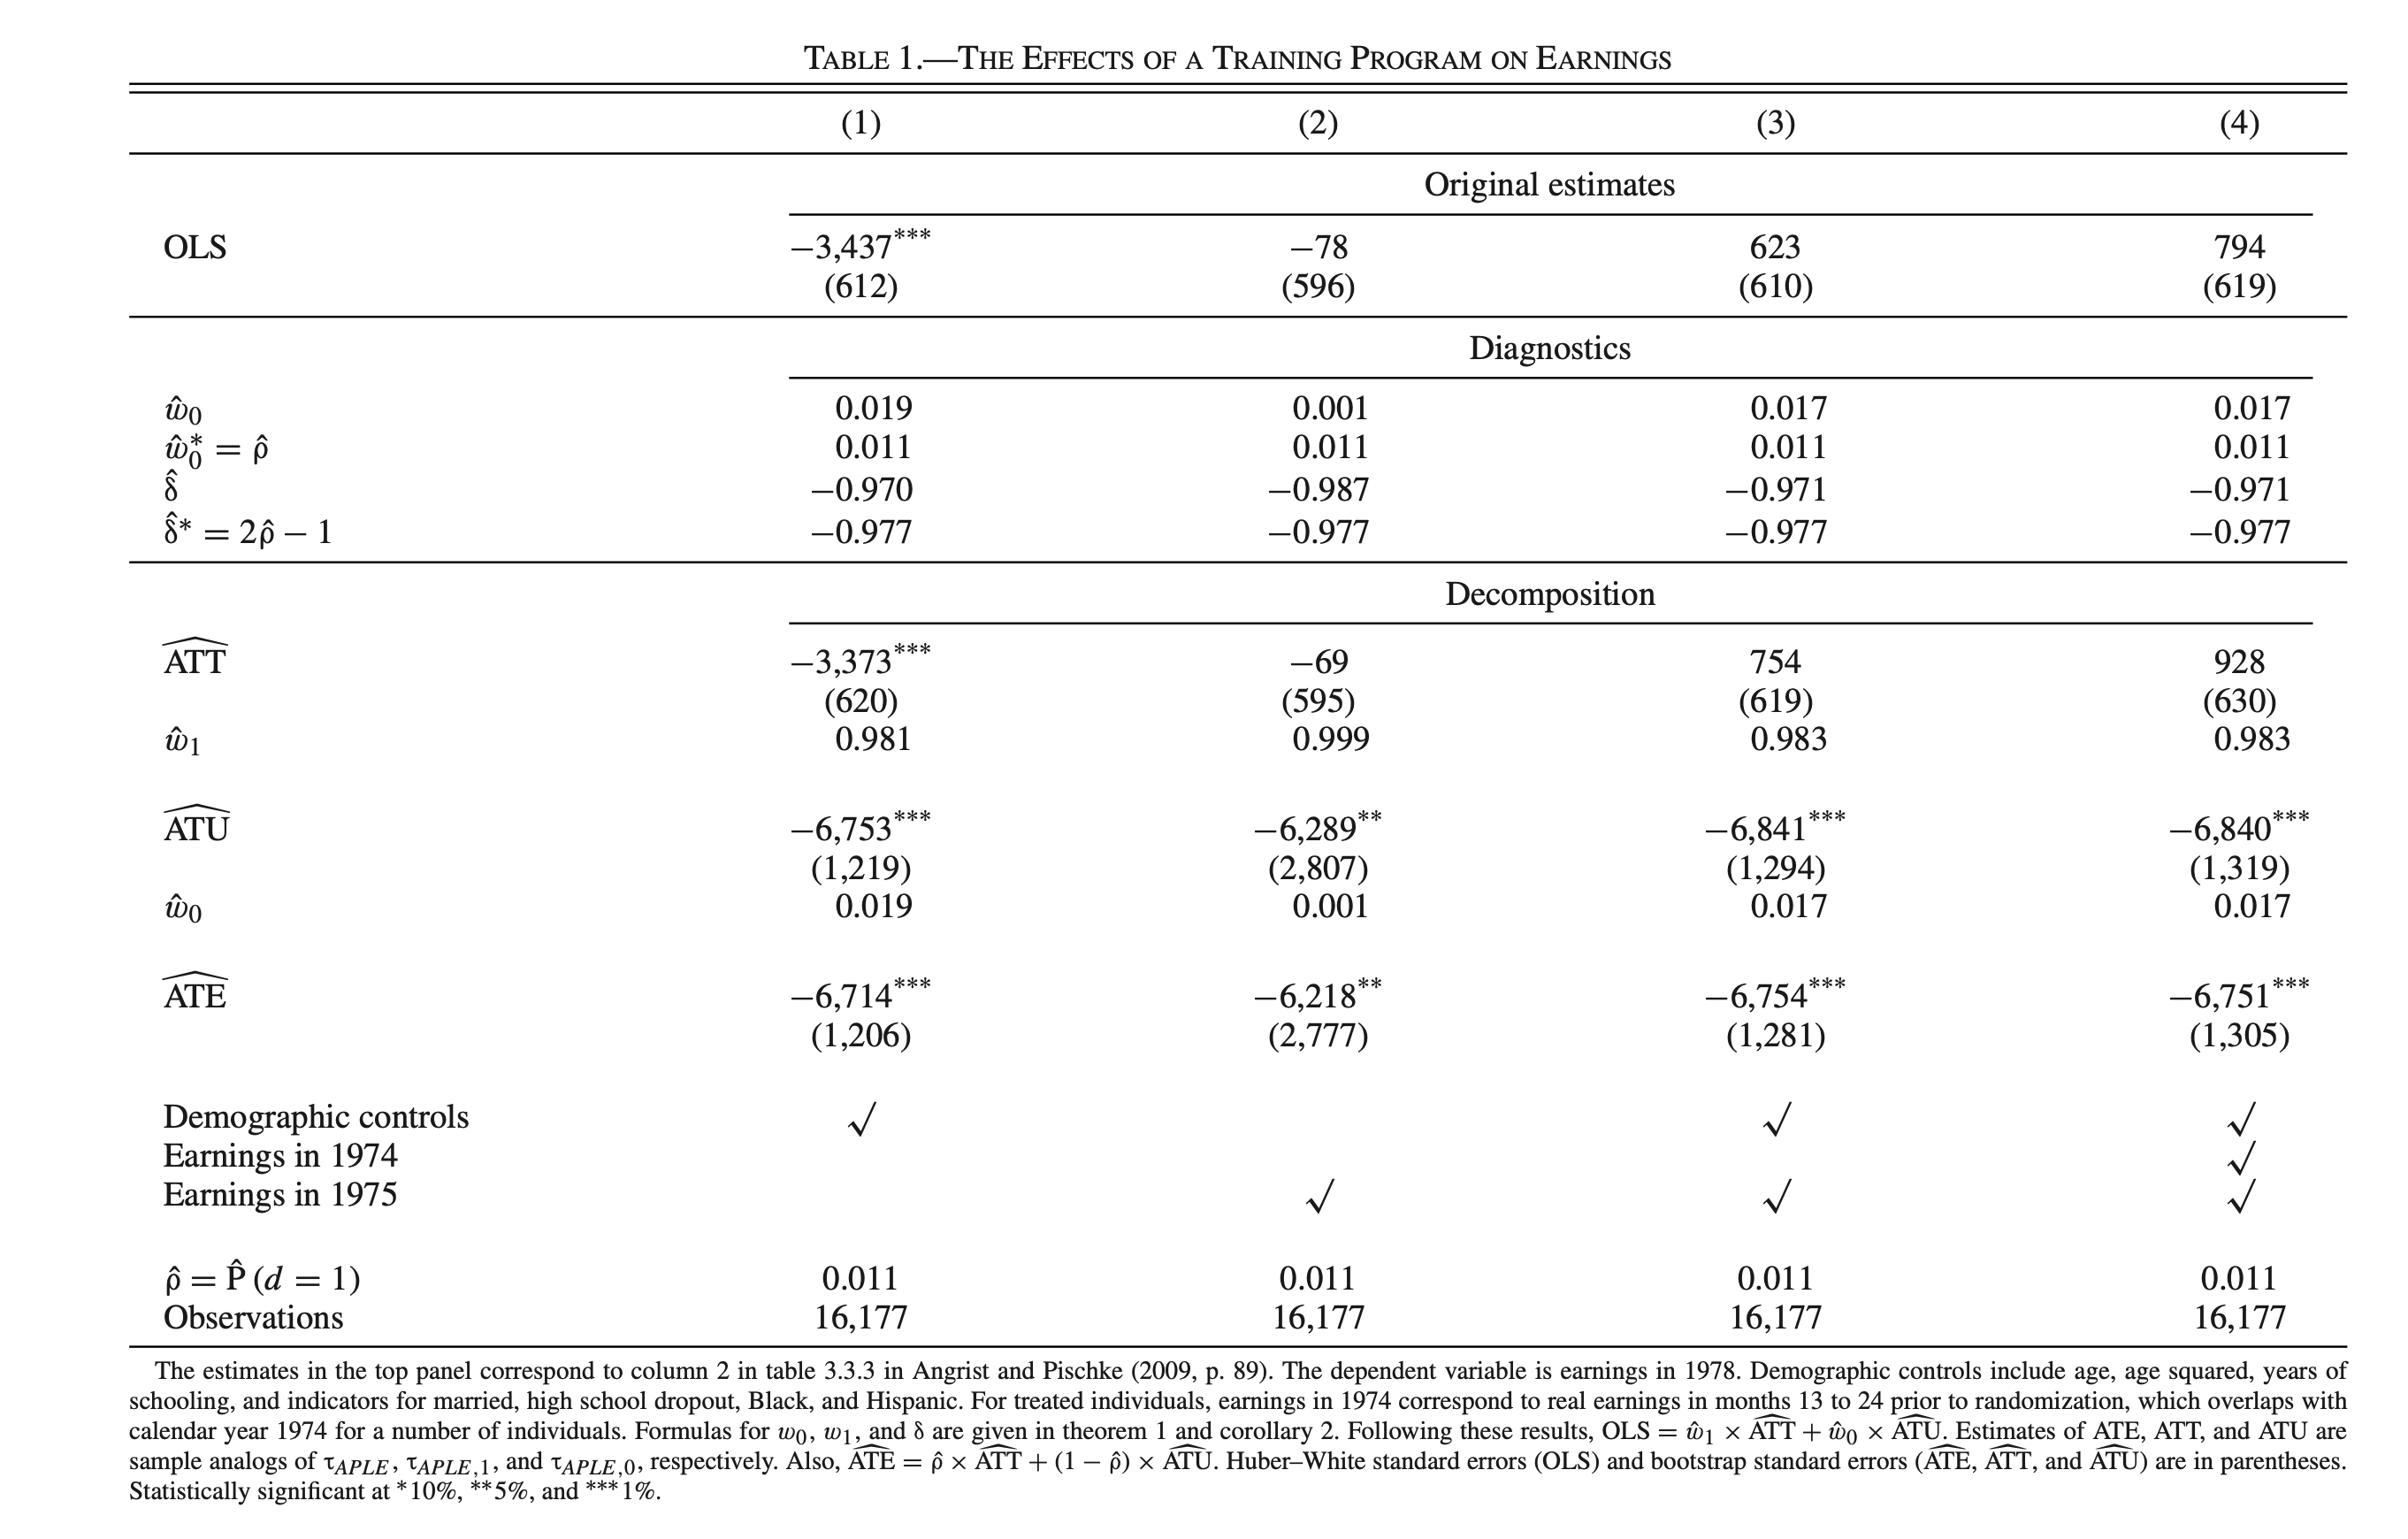
\includegraphics[width=0.8\textwidth]{./lecture_includes/tymon_lalonde_table1.png}
    \end{figure}
\end{frame}

\begin{frame}{Stata simulation}

Let's do this ourselves using lalonde.do in the labs/matching on github repo

\end{frame}


\begin{frame}
\frametitle{Replications of Lalonde data using Dehejia and Wahba sample with CPS control}

\tiny
\begin{tabular}{lccccc}
\hline \hline
 & \multicolumn{5}{c}{Dependent variable: Real earnings in 1978} \\
 & (1) & (2) & (3) & (4) & (5) \\
Controls: & No controls & Demographics & RE75 Only & Demo and RE75 & Demo, RE74 and RE75 \\
\hline
Treatment                 &   -8497.516***&   -3436.795***&     -77.705   &     622.547   &     \textbf{793.587}   \\
                    		&   (581.916)   &   (612.056)   &   (596.215)   &   (609.582)   &   (618.609)   \\
\hline \end{tabular}

\bigskip

Each column corresponds to a set of observable controls below:
\begin{itemize}
\item Demographics: Age, Age-squared, Years of schooling, Marriage dummy, High school dropout dummy, Black and Hispanic dummies
\item Real earnings in 1975 (RE75)
\item Real earnings in 1974 (RE74)
\end{itemize}

Our focus will be on the last estimate.  Question is what is this?

\end{frame}



\begin{frame}
\frametitle{Regression Adjustment Application and Results}
\begin{itemize}
  \item Estimate the regression adjustment method interacting treatment with all covariates to recover estimates of all parameters:
    \begin{itemize}
      \item \( \widehat{ATE} = -\$4,930 \)
      \item \( \widehat{ATT} = \$796 \)
      \item \( \widehat{ATU} = -\$4,996 \)
    \end{itemize}
  \item OLS estimate \( \$794 \) shows a weight on ATT nearly 100\%, reflecting the treated sample's size of 1.1\%
  \item Illustrates "weight reversal''  principle: OLS weights do not reflect expected proportions.
\end{itemize}
\end{frame}

\begin{frame}
\frametitle{General Implications of the OLS Weight Anomaly}
\begin{itemize}
  \item The NSW example generalizes beyond this specific case.
  \item OLS weights can misrepresent effects, influenced by treatment group proportion.
  \item OLS estimand does not always align with intuitive weight distributions for ATT and ATU.
\end{itemize}
\end{frame}

\begin{frame}{Concluding remarks}

\begin{itemize}

\item Last years have shown a \emph{particular} OLS specification yields biased estimates of all causal parameters when there exists heterogeneity in the treatment effects
	\begin{itemize}
	\item Goodman-Bacon (2021) for instance showed this with the common twoway fixed effects specification and dynamic treatment effects
	\end{itemize}
\item Turns out it was not a diff-in-diff problem only -- it's an OLS problem more generally
	\begin{itemize}
	\item We saw it also in a paper by Goldsmith-Pinkham, Hull and Kolsar on contamination bias in linear models with multiple treatment effects and heterogeneity
	\end{itemize}
\item Here we see the perversity of the effects under unconfoundedness and heterogeneity which is the OLS coefficient counterinuititvely favors the smaller groups and therefore their causal parameters
\end{itemize}

\end{frame}

\begin{frame}{Concluding remarks}

\begin{itemize}

\item We mentioned work by Anna Aizer more likely is estimating coefficients that are more like the ATU than either the ATE or the  ATT because of how large the treatment group is
\item This has implications for analysis in which the proportion of groups differ in size due to population differences or over-representation of one group over another (i.e., Asians in criminal justice)
\item The smaller the group, the larger their influence on the OLS coefficient
\item Lesson here is that regression adjustment as well as nearest neighbor matching with bias adjustment may need to be your core models, not the additive in covariates OLS specification we are accustomed to

\end{itemize}

\end{frame}




\section{Concluding remarks}



\begin{frame}{Comments}


\begin{itemize}

\item Unconfoundedness means that the confounders are known and quantified, meaning they're in your data and well measured
\item Also means that within the dimensions of those covariates is an RCT (``independence'')
\item Common support is also needed with matching, but for OLS you rely on extrapolation and functional forms
\item Without a prior behavioral model guiding you, it's very hard to defend unconfoundedness (identification by convenience) 

\end{itemize}

\end{frame}

\begin{frame}{When not to use unconfoundedness methods}

\begin{itemize}
\item Individual sorting based on rationality is strong and subtle
	\begin{itemize}
	\item May be easier to defend in some situations though -- we are studying the effect of a prison assignment where if you get a suicide risk score, a team of trained inmates go meet you
	\item Only happened in 16 prisons -- I have 84 others and I know each inmate score
	\item They are picking their score to a degree, by picking their suicidality, but you wouldn't say it was done \emph{rationally}
	\end{itemize}
\item College attendance, major, marriage, children, divorce -- very hard to imagine that for people with identical covariate values they all flipped coins
\item Unconfoundedness is a strong assumption, and the weaker ones (like with respect to $Y^0$) may be easier to defend which gets you to the ATT

\end{itemize}

\end{frame}  

\begin{frame}{Common Support}

\begin{itemize}
\item Unconfoundedness says on average, $E[Y^0|D=1,X]=E[Y^0|X]$ -- that is, it doesn't depend on $D$ so you can just switch the known for unknown ones
\item But even if unconfoundedness holds doesn't mean your dataset is large enough that the one to one matches can happen -- that's failure to have enough matches because the dimensions are too large
\item So much of the literature is how to handle failed common support
\item Bias adjustment methods are one way to address that but even they can't work miracles
\end{itemize}

\end{frame}





\begin{frame}{My opinions: Parameter first}

\begin{itemize}

\item You have three average causal effects associated with three populations
\item You will need up front to choose which one, and justify why that is the one you want
\item The conditional ATEs like ATT or ATU have fewer assumptions
\item ATT is often the one you want anyway (e.g., effect of discrimination on blacks not everyone)
\end{itemize}

\end{frame}

\begin{frame}{My opinions: Regression}

\begin{itemize}
\item Simple regression model $$Y_i = \alpha + \delta D_i + \beta X_i +\varepsilon_i$$
\item It requires extremely strong assumptions like constant treatment effects and has weird weighting properties as we discussed
\item Functional form must be right also (linearity)
\item It is simply unnecessary to estimate this any longer
\end{itemize}

\end{frame}

\begin{frame}{Remember Imbens and Rubin}

\begin{itemize}

\item  Additive OLS model with exogeneity imposes strong assumptions on the DGP: constant treatment effects, unconfoundedness and functional form assumptions
\item Matching allows for heterogenous treatment effects but requires common support; OLS uses extrapolation in its place
\item You can address heterogenous treatment effects with fully interaction called regression adjustment (itself extremely uncommon in practice), but that does not address nonlinear DGP

\end{itemize}

\end{frame}

\begin{frame}{Quote that great Tymon Sloczynski quote (Restat 2022)}

\footnotesize
\begin{quote}
``An important motivation for using $Y=\alpha + \delta D + \beta X + \varepsilon$ and OLS is that the linear project of $Y$ on $D$ and $X$ provides the best linear predictor of $Y$ given $D$ and $X$ (Angrist and Pischke 2009). However if our goal is to conduct causal inference, then this is not, in fact, a good reason to use this method.  Ordinary least squares is ``best'' in predicting actual outcomes, but causal inference is about predicting missing [fictional] outcomes. In other words, the OLS weights are optimal for predicting ``what is''.  Instead, we are interested in predicting ``what would be'' if treatment were assigned differently.'' (Tymon Sloczynski, Restat 2022)
\end{quote}

\bigskip


\end{frame}


\begin{frame}{My opinions: Regression adjustment}

\begin{itemize}
\item If you want to estimate something with a regression, then assuming unconfoundedness and linearity you can using regression adjustment (RA)
\item Recall: regression adjustment allows you to estimate both the ATE and the ATT but will require a saturated model
\item You'll want to use software for this as it's too easy to make a mistake
\end{itemize}

\end{frame}

\begin{frame}{Nearest neighbor matching with bias adjustment}

\begin{itemize}
\item Consider Abadie and Imbens (2006; 2008; 2011) nearest neighbor and minimize the Mahanalohbis distance metric
\item This only requires unconfoundedness and common support, not constant treatment effects and not parametric functional form like regressions 
\item But most likely you will not have common support, so consider an outcome regression adjustment called bias adjustment

\end{itemize}

\end{frame}

\begin{frame}{Inverse probability weighting}

\begin{itemize}
\item If you use propensity scores, then consider using the IPW as it's got fewer ad hoc choices and does not require knowing the true propensity score (for efficiency)
\item You may want to also use outcome regression or double robust to correct for any model misspecification (consistency)
\item Always plot the propensity score histograms and assess overlap for the parameter you want
\end{itemize}

\end{frame}



\end{document}
\begin{frame}{M-bias as collider}



  \centering
  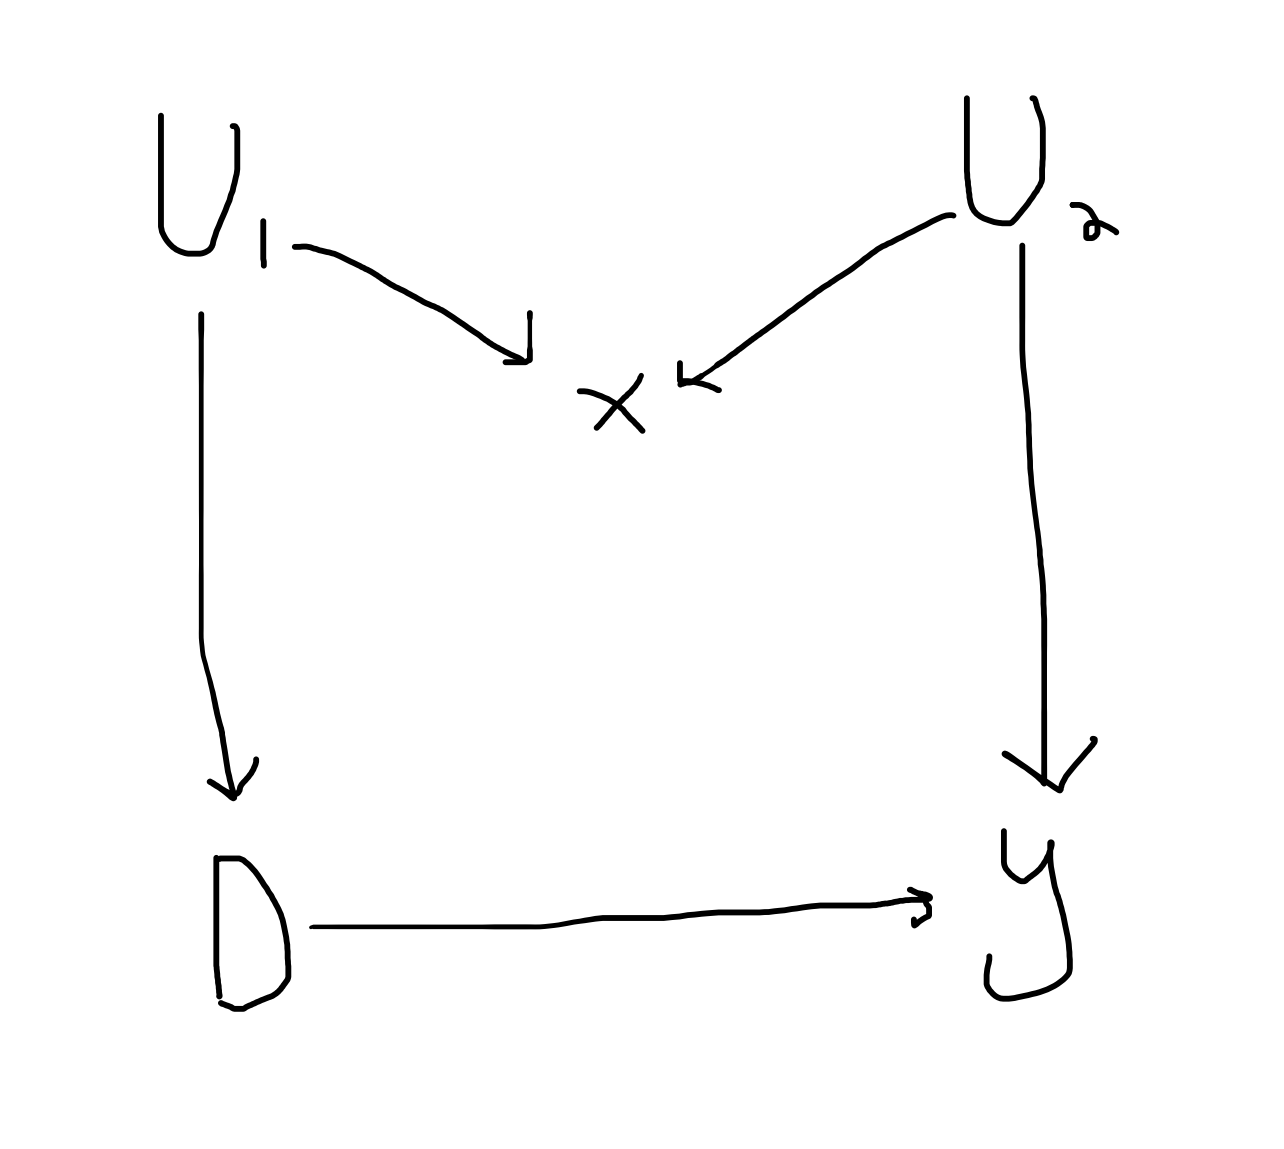
\includegraphics[scale=0.5,height=6.5cm, width=10cm]{./lecture_includes/mbias}

\footnotesize
$X$ is pre-treatment, but if you conditioned on it, then $D\leftarrow U1 \rightarrow \mbox{X} \leftarrow U2 \rightarrow Y$ and $X$ is a collider. Colliders take strange forms, so the conditioning set \emph{must} be thoughtfully chosen based on being a strong predictor of $Y^0$, preferably based on expert knowledge and not a kitchen sink of all available regressors

\end{frame}


